
\newcommand{\beispiel}[1]{
 \vspace{0.7em}
 \noindent
 \textit{#1:}
 \vspace{-0.2em}

 \noindent
}

\providecommand{\tilV}{\tilde{V}}

\hyphenation{Er-war-tungs-wert}
\hyphenation{Aus-wahl-wahr-schein-lich-kei-ten}
\hyphenation{gleich-zei-tig}
\hyphenation{ent-spre-chen}
\hyphenation{zwei-stu-fig}
\hyphenation{In-klu-sions-wert}

%#######################################
\chapter{\label{sec:choice}Modelle diskreter Entscheidungen}
%#######################################
%\red{Siehe vkoek\_Teil4.README}

%#######################################
\section{\label{sec:DiscrEinf}Einf\"uhrung}
%#######################################

Viele Sachverhalte der Verkehrs\"okonometrie betreffen
\bfdef{diskrete Entscheidungen}, d.h. man muss sich f\"ur eine aus
\"ublicherweise wenigen Alternativen entscheiden. Das wird deutlich,
wenn man das bereits in Kap \ref{sec:Allg} besprochene
 klassische Vierstufenmodell der Verkehrsplanung
unter dem Gesichtspunkt der anfallenden
 Entscheidungen betrachtet (Abb. \ref{fig:vierstufenmodellDiscr}):

%###########################################
%\begin{figure}[t!]
\begin{figure}[h!]
\fig{1.0\textwidth}{figsDiscr/vierstufenmodellDiscr.eps}
\caption{\label{fig:vierstufenmodellDiscr}Das klassische Vierstufenmodell
der Verkehrsplanung als Beispiel diskreter Entscheidungen (siehe den Haupttext).
}
\end{figure}
%###########################################

\bi
\item Zun\"achst wird in der \bfdef{Aktivit\"atenwahl} (fr\"uhmorgens
oder auch Tage davor) festgelegt, was denn das heutige ``Tagewerk''
sein soll: Dies betrifft insbesondere wahlfreie Aktivit\"aten wie
Einkaufen gehen, zum Sport gehen usw.
\item In der darauffolgenden \bfdef{Zielwahl} wird entschieden,
\textit{wo} die gew\"ahlten Aktivit\"aten stattfinden sollen
(z.B. in welchen L\"aden eingekauft werden soll) 
\item Danach oder gleichzeitig wird in der \bfdef{Verkehrsmittelwahl}
entschieden, \textit{wie} die Ziele der jeweiligen Aktivit\"aten
erreicht werden sollen: Zu Fu\3, mit dem Rad, mit Bus oder Bahn (\"OV), 
Auto oder Motorrad (MIV), mit dem Flugzeug usw. 
\item Schlie\3lich wird in der \bfdef{Routenwahl} der g\"unstigste
Weg f\"ur das gew\"ahlte Ziel und das gew\"ahlte Verkehrsmittel 
im Streckennetzwerk ausgesucht.
\ei
%
%###########################################
%\begin{figure}[t!]
\begin{figure}[t!]
\fig{0.65\textwidth}{figsDiscr/zweiAlternat-U.eps}
\caption{\label{fig:zweiAlternat-U}Indifferenzkurven einer linearen,
von zwei exogenen Variablen abh\"angigen Nutzenfunktion. Die Symbole
bezeichnen die Lage bestimmter Alternativen im Raum der exogenen
Variablen.
}
\end{figure}
%###########################################
%
Grunds\"atzlich sind diskrete Entscheidungen nichtlinear, was nun 
anhand Abb. \ref{fig:zweiAlternat-U} verdeutlicht wird. In der
dargestellten Situation gibt es als ma\3gebliche  exogene Variable
(Beeinflussungsfaktoren) die komplexe
Reisezeit $T$ und die Kosten $K$. Diese k\"onnen jeweils 
 f\"ur die beiden in Frage kommenden
Alternativen ``\"OV'' und ``MIV'' berechnet werden und dienen als
Kriterien f\"ur die Wahlentscheidung (endogene Variable). 
Im einfachsten Fall bildet man aus $T$ und $K$ f\"ur jede Alternative eine lineare
Nutzenfunktion, 
\be
\label{Vlin}
V_i=\beta_1 T_i + \beta_2 K_i,
\ee
berechnet diese  f\"ur beide Alternativen und w\"ahlt 
 gem\"a\3 dem klassischen \"okonomischen Modell der Nutzenmaximierung
(\textit{Homo Oeconomicus}):
\be
\label{igewaehlt}
i\sub{gew\"ahlt}=\text{arg}(\max_i(V_i))
\ee
die Alternative mit dem gr\"o\3eren Nutzen.\footnote{Die
Argumentfunktion arg(.) in Gl. \protect\refkl{igewaehlt} bezeichnet
den zum Maximum bzw. Minimum in der Klammer geh\"origen Wert des
zu maximierenden (minimierenden) Arguments.}
In der den Raum der exogenen Variablen darstellenden Abbildung
\ref{fig:zweiAlternat-U}  werden beide Alternativen durch je einen
Punkt repr\"asentiert. Ferner sind \bfdef{Indifferenzkurven} gleichen
Nutzens eingezeichnet, die mit \refkl{Vlin} nat\"urlich zu Geraden
degenerieren. Gew\"ahlt wird nun die Alternative, welche sich bez\"uglich
der Indifferenzkurven weiter ``links unten'' befindet, da in
dieser Richtung der Nutzen zunimmt bzw. die generalisierten Kosten
abnehmen.

Sei Anfangs ($t=t_0$) die Situation so, dass der MIV bevorzugt
wird. Nun steigen die Kraftstoffkosten, so dass f\"ur den MIV die
Kosten steigen, w\"ahend alles andere (die Reisezeiten und die Kosten
f\"ur den \"OV) unver\"andert bleibt
(\textit{ceteris paribus}). Zum Zeitpunkt $t_1$ ist aber immer noch
$V\sub{MIV}>V\sub{\"OV}$, so dass nach wie vor der MIV gew\"ahlt
wird. Trotz \"Anderung der exogenen Variablen $K\sub{MIV}$ \"andert
sich also nichts bei der endogenen Variablen der
Wahlentscheidung. Erst wenn zum Zeitpunkt $t_2$ die Kosten
$K\sub{MIV}$ noch einmal um den gleichen Betrag erh\"oht werden,
schl\"agt die Entscheidung zugunsten des \"OPNV um. 


%###########################################
%\begin{figure}[h!]
\begin{figure}[t!]
\fig{0.95\textwidth}{figsDiscr/zweiAlternat-P.eps}
\caption{\label{fig:zweiAlternat-P}Die zu der in
Abb. \protect\ref{fig:zweiAlternat-U} dargestellten Nutzenfunktion
geh\"orige Wahlentscheidung f\"ur den \"OPNV
in Abh\"angigkeit der (Treibstoff-)kosten $K\sub{MIV}$ f\"ur den MIV
unter \textit{ceteris paribus} Bedingungen. Auf Individualebene lautet
die Entscheidung nur ja (1) oder Nein (0); Auf Kollektivebene bzw. bei
Zufallselementen in der Nutzenfunktion ergibt sich eine
Wahrscheinlichkeit zwischen 0 und 1. Die drei Zeitpunkte bzw. die
dazugeh\"origen Werte von $K\sub{MIV}$ entsprechen
denen in Abb.  \protect\ref{fig:zweiAlternat-U}.
}
\end{figure}
%###########################################

Bei ein und
derselben \"Anderung der exogenen Variablen tut sich also einmal
nichts, w\"ahrend es im anderen Fall eine dratische \"Anderung
gibt. Dieses typische Merkmal einer Nichtlinearit\"at bleibt auch bei
mehr als zwei Alternativen erhalten. Betrachtet man statt der
\textit{Individualebene} die \textit{Kollektivebene}, also
unterschiedliche Pr\"aferenzen der einzelnen Entscheider, so weicht
die ``Sprungfunktion'' der Alternativenwahl zwar 
auf, bleibt aber im Wesentlichen nichtlinear
(Abb. \ref{fig:zweiAlternat-P}). Die im vorhergehenden Kapitel
entwickelten m\"achtigen Werkzeuge der multivariaten linearen Modelle
sind also nicht einsetzbar, wenn man nicht den speziellen Mechanismus
der \bfdef{logistische Regression} nutzt, der aber nicht gut
verallgemeinerbar ist. 

\maintext{Auch bei linearen Nutzenfunktionen sind die Modelle der
diskreten Wahltheorie prinzipiell nichtlinear. Dies gilt auch auf der 
Kollektivebene.
}


%#######################################
\section{\label{sec:discrMath}Mathematische Beschreibung}
%#######################################
Diskrete Wahlentscheidungen werden heutzutage 
(und auch in diesem Skript) im Allgemeinen durch Maximierung  einer
aus deterministischen und Zufallsanteilen bestehenden Nutzenfunktion
(\emph{Homo Oeconomicus}) hergeleitet. Es geht jedoch auch anders:
Bereits 
1927\footnote{ L.L. Thurstone, The American Journal of Psychology
  \textbf{38}, 3, pp. 368 (1927).} wurde 
ein bestimmtes Modell, das \emph{binomiale Probitmodell}
(Abschnitt~\ref{sec:ProbitBinom}), anhand der Modellierung 
psychologischer Stimuli hergeleitet. Erst 1960
 wurden diese Stimuli
als Ergebnis der Maximierung einer Nutzenfunktion
uminterpretiert.\footnote{Marschak, J. \textit{Binary Choice Constraints and
  Random Utility Indicators},  Stanford 
Symposium on Mathematical Methods in Social Science, Edited by K. Arrow.
Stanford, CA: University of Stanford 1960.} 
In systematischer Weise
wurde die \bfdef{diskrete
Wahltheorie} (engl. \textit{discrete-choice analysis}), insbesondere
das heute am gebr\"auchlichste \emph{Logit-Modell}, 
in den Siebziger und Achziger 
Jahren von Daniel
McFadden\footnote{D. McFadden, \textit{Conditional logit analysis of
  qualitative choice behavior}, Institute of Urban and Regional
  Development, University of California (1973).} (Nobelpreis 2000),
 Ben-Akiva
\footnote{Moshe Ben-Akiva and Steven Lerman, \textit{Discrete Choice Analysis
Theory and Application to Travel Demand}. MIT Press (1985).} 
und anderen entwickelt. 
%Aber auch das Logit-Modell kann auf ganz anderem
%Wege, \"uber 

In jedem Fall werden die
 Modelle der diskreten Wahltheorie grunds\"atzlich
``mikroskopisch'' formuliert, also Einzelentscheidungen individueller
Personen $i$ betrachtet. Man kann auch bez\"uglich der Entscheidung
verhaltenshomogene  Gruppen zusammenfassen. Ein Beispiel einer solchen
Gruppe im Falle der Verkehrsmittelwahl sind alle weiblichen
Erwerbst\"atigen in der Grundgesamtheit bzw. Stichprobe, welche 
zwischen 30 und 40 Jahren alt sind, kein Kfz aber ein Rad zur
Verf\"ugung haben,
und bei denen die Entfernung Wohnung-Arbeitsst\"atte zwischen 5 und 10
km betr\"agt. Der Personenindex wird dann zum Personengruppenindex,
aber die Entscheidung wird nach wie vor individuell (d.h. Person f\"ur
Person) modelliert.

%###########################################
%\begin{figure}[h!]
\begin{figure}[t!]
\fig{0.95\textwidth}{figsDiscr/discrKomp.eps}
\caption{\label{fig:discrKomp}Die wichtigsten Komponenten von
\textit{discrete-choice} Modellen. In blau stehen Beispiele f\"ur die
Verkehrsmittelwahlentscheidung. 
}
\end{figure}
%###########################################

Modelle der diskreten Wahltheorie haben zwei Hauptkomponenten
(Abb. \ref{fig:discrKomp}): 

\bi
\item F\"ur jede Person und jede Alternative gibt es eine deterministische
Nutzenfunktion (Abschnitt \ref{sec:discrV}). Diese h\"angt  von den in Abschnitt
\ref{sec:discrExogen} besprochenen exogenen Variablen ab und kann
linear, quasilinear oder nichtlinear sein.
\item Ein Wahlmodell beschreibt die vom deterministischen
Nutzen und einem modell\-abh\"angigen Zufallsnutzen 
abh\"angige Wahlentscheidung  bzw. die
Auswahlwahrscheinlichkeiten der m\"oglichen Alternativen.
(Abschnitt~\ref{sec:discrEntsch}).
\ei
Da grunds\"atzlich rationale Entscheidungen angenommen werden 
(\textit{homo oeconomicus}, der Gesamtnutzen wird maximiert), 
 ist das Wahlmodell \"aquivalent zur
Definition des Verteilung des Zufallsnutzens. Wichtig sind 
normalverteilte Zufallsnutzen, welche zu den \bfdef{Probit-Modellen}
f\"uhren (Abschnitt \ref{sec:Probit}) und extremwertverteilte
(genauer: gumbelverteilte)
Zufallsnutzen, welche den in Abschnitt \ref{sec:Logit} behandelten \bfdef{Logit-Modellen}
entsprechen. Beide Ans\"atze haben Vor- und Nachteile: Probit-Modelle
erlauben allgemeine Korrelationen und unterschiedliche Varianzen
(\bfdef{Heteroskedastizit\"at}) und sind statistisch begr\"undet
(Zentraler Grenzwertsatz), aber ihre Auswahlwahrscheinlichkeiten sind
i.A. nur durch Simulation bestimmbar. Hingegen ist die
Logit-Auswahlwahrscheinlichkeit eine einfache Formel, aber es m\"ussen
identisch-unabh\"angige (Gumbel-)Verteilungen der Zufallsnutzen
angenommen werden.

Oftmals ist aber die Annahme unabh\"angiger und/oder
identisch verteilter (i.i.d.) Zufallsnutzen aus dem Sachverhalt heraus
nicht zu halten ,
z.B. bei der kombinierten Verkehrsmittel- und Routenwahl. Will man auf
die analytische Berechnung der Auswahlwahrscheinlichkeit nicht
verzichten, kommen \bfdef{Generalized
  Extreme Value (GEV)} Modelle zum Einsatz (Abschnitt~\ref{sec:GEV}). Diese erlauben -- mit
Einschr\"ankungen -- korrelierte und heteroskedastische Zufallsnutzen,
die einer verallgemeinerten Extremwertverteilung
gen\"ugen.\footnote{Die Einschr\"ankung auf eine bestimmte Form der
  Verteilung, z.B. Gumbel statt Gau\3, ist selten relevant, da die
  Dichtefunktionen \"ahnlich aussehen. Wichtiger sind die
  Korrelationen und die Heteroskedastizit\"at.} Ein besonders
wichtiger und anschaulicher Spezialfall der GEV-Modelle sind die 
 \bfdef{Nested-Logit Modelle} (Abschnitt~\ref{sec:nestedLogit}).

Zun\"achst gilt es aber, die mathematische Beschreibung der
Alternativen und der exogenen Variablen 
in eine Form zu bringen, auf die Wahlmodelle angewandt
werden. Dies wird zun\"achst betrachtet.

%#######################################
\subsection{\label{sec:discrAltern}Alternativen}
%#######################################

Jede Person bzw. Personengruppe $n$ hat bei der Wahlentscheidung im Allgemeinen
unterschiedliche \bfdef{Alternativenmengen} $A_n=\{a_{ni}\}$ zur
Verf\"ugung.\footnote{In der Literatur zur diskreten Wahltheorie
  werden die einzelnen Datens\"atze durch die Bank mit dem Index $n$
  (statt $i$ wie bei der Regressionsrechnung) bezeichnet, w\"ahrend
  $i$ nun den \emph{Alternativenindex} bezeichnet. Zur
  leichteren Vergleichbarkeit folgen wir der Konvention (eine
  \"Ubersicht der Bezeichnungen findet sich in
  Abschnitt~\ref{sec:discrSymbols}).}
 Legt man fest, dass ein bestimmter Index $i$ eine
bestimmte feste Alternative bedeutet, entspricht die Menge $A_n$ also
einer Menge von nat\"urlichen Zahlen $\{i\}$ im Bereich von 1 bis
$I$. Um die ``Buchhaltung'' nicht durch unterschiedliche Alternativenmengen 
zu verkomplizieren, werden f\"ur nicht verf\"ugbare Alternativen 
sehr hohe  ``virtuelle Strafkosten''bei den deterministischen
Nutzenfunktionen veranschlagt, so dass die Wahrscheinlichkeit, solche
Alternativen zu w\"ahlen, 
\textit{de facto} gleich Null ist.\footnote{Im Logit-Modell
f\"uhrt ein ``Malus'' von 1000 gegen\"uber einer anderen Alternative 
zu einer Auwahlwahrscheinlichkeit der Gr\"o\3enordnung 
$e^{-10^3}$ (nach dem ``Null Komma'' stehen etwa 400 Nullen, ehe
eine signifikante Ziffer kommt.)}
Die Alternativen m\"ussen folgenden Bedingungen gehorchen:
\benum
\item \emph{exklusiv} bzw. \emph{nicht-h\"aufbar}: Es kann h\"ochstens
  eine gew\"ahlt werden.
\item \emph{vollst\"andig}: Es muss mindestens
  eine gew\"ahlt werden. Ber\"ucksichtigt man Punkt~1,  muss also
  genau eine gew\"ahlt werden,
\item sie m\"ussen \emph{wesentlich voneinander verschieden} sein,
\item und es darf nur \emph{endlich viele} Alternativen geben.
\eenum

\subsubsection*{Beispiel Verkehrsmittelwahl:}
Punkt 1 impliziert, dass man nicht fragen sollte ``welches
Verkehrsmittel verwendeten Sie f\"ur Ihren Weg hierher'' (mit der
m\"oglichen Antwort ``kombiniert Rad, 
\"OV und zu Fu\3'', wenn man mit dem Rad zur Haltestelle f\"ahrt und
an der Zielhaltestelle zu Fu\3 zum Ziel l\"auft), sondern beispielsweise
``welches Hauptverkehrsmittel verwendeten Sie''.

 Punkt~2 impliziert,
dass man, speziell bei Stated-Choice Analysen,  ggf eine
``Nicht-Alternative'' (``unter diesen Bedingungen bleibe ich zu
Hause'') anbietet, und bei Revealed-Choice Fragen eine Alternative
``sonstige Verkehrsmittel'' vorsieht, die Motorradfahrer,
Hubschrauberflieger, Inline-Skater etc. ber\"ucksichtigt. 

Punkt~3  ist
erforderlich, um  Verzerrungen zu
vermeiden, speziell bei Stated Choice: Dies wird am deutschlichsten am
Beispiel des bekannten \bfdef{Red-Bus Blue-Bus Problems}: 
Lauten die vier Alternativen bei einem zu Fu\3 unpraktikablem Weg
``Rad'', ``Roter Bus'', ``Blauer Bus'', ``Kfz'', so sind (au\3er
bei Leuten, die rot oder blau hassen) die deterministischen
Nutzenfunktionen des roten und blauen Busses gleich. Damit werden
vom Modell Busse doppelt gez\"ahlt und die Wahrscheinlichkeit, Busse
zu w\"ahlen, \"ubersch\"atzt (oder, wenn man dieses Modell kalibriert,
die Attraktivit\"at von roten oder blauen Bussen bzw. deren
Nutzenfunktionen gegen\"uber sonstigen
Verkehrsmitteln untersch\"atzt). Sind insbesondere alle vier
deterministischen Nutzenfunktionen gleich, so w\"urde der \"OV, also
einer der Busse, mit einer Wahrscheinlichkeit von 1/2 gew\"ahlt,
obwohl eigentlich 1/3 plausibel w\"are.

In der Regel sind nur
\emph{Verkehrssysteme} (zu Fu\3, Rad, \"OV, MIV) wesentlich
verschieden, in speziellen Untersuchungen k\"onnen aber durchaus Bus
und Bahn als eigene Alternativen gelten.

Punkt~4 schlie\3t kontinuierliche Wahlentscheidungen wie die Wahl der
Wunsch\-geschwin\-digkeit auf freier Strecke aus. Einerseits werden kontinuierliche
Wahlentscheidungen aber durch eine metrische endogene
Variable beschrieben und sind der Regressionsrechnung
zug\"anglich. Andererseits kann man die Menge der m\"oglichen
Wunschgeschwindigkeiten in einen vollst\"andigen Satz einander
ausschlie\3ender Teilmengen ($<\unit[80]{km/h}$, \unit[80-100]{km/h}
usw.) aufspalten und jede Teilmenge einer Alternative zuordnen, so dass alle vier Punkte 
erf\"ullt sind.

\verstaendnisbox{Welche Kriterien sind verletzt, wenn man die
  Wunschgeschwindigkeiten in f\"unf Teilmengen
$<\unit[80]{km/h}$, \unit[80-100]{km/h}, \unit[100-120]{km/h},
  \unit[120-121]{km/h}, \unit[121-140]{km/h} aufspaltet? Beg\"undung?
}



%#######################################
\subsection{\label{sec:discrExogen}Beeinflussungsfaktoren}
%#######################################

Wie in allen \"okonometrischen Modellen werden Beeinflussungsfaktoren
als exogene bzw. Input-Variable modelliert. Man unterscheidet dabei zwei
Kategorien:

\bi
\item Faktoren, welche im wesentlichen Eigenschaften der
Alternativen darstellen,  werden durch 
einen Satz von \bfdef{generischen Variablen}, sog. \bfdef{Charakteristika}
$\vec{C}_{ni}=\{C_{jni}\}, j=1, ..., J_C$ modelliert. Dieser Satz von Faktoren
(repr\"asentiert durch einen  Vektor und dargestellt in Fettdruck) 
h\"angt naturgem\"a\3 von der Alternative $i$, aber h\"aufig  auch 
von der Personen(gruppe) $n$ ab (z.B. bei der Reisezeit als typischen Vertreter
dieser Art von Variablen). Es gibt allerdings auch generische Variable
(z. B. Preise von Produkten bei einer Produktwahlentscheidung), welche
im wesentlichen f\"ur alle Personen denselben Wert
aufweisen.\footnote{Wenn man von den immer beliebteren Kundenkarten absieht.}

\beispiel{Beispiel Verkehrsmittelwahl ($i=1$: zu Fu\3, 2: Rad, 3:
  \"OV, 4: MIV)}
\bdma
C_{1ni} &=T_{ni} & \text{Komplexe Reisezeit (in Minuten)}\\
C_{2ni} &=K_{ni} & \text{Kosten (in \euro{})}\\
C_{3ni} &=\sqrt{V(T_{ni})} & \text{Zuverl\"assigkeit
(Standardabweichung von $T$  in Minuten, siehe Abschnitt~\ref{sec:zuverl})}\\
C'_{3ni} &=T_{0.95} & \text{Alternativ:
95. Perzentil der Reisezeit} \\
C_{4ni} &=B_{ni} & \text{Quantifizierte Beqemlichkeit ...}
\edma
Beispielsweise w\"urde $C_{123}=T_{23}$ die komplexe
(Haust\"ur-zu-Haust\"ur-) Reisezeit (Kriterium bzw. Faktor $j=1$)
f\"ur Person(nengruppe) $n=2$ bedeuten, 
wenn sie mit dem \"OV (Alternative $i=3$) f\"uhre.

\item Rein personenbezogene Faktoren werden durch
 einen Satz von 
\bfdef{sozio\-\"okono\-mischen Variablen} $\vec{S}_n=\{S_{jn}\}, j=1,
..., J_S$
modelliert. Als personenspezifische Merkmale h\"angen die $\vec{S}_n$ 
\emph{nur} von der Person, nicht aber von der
Alternative ab.

\beispiel{Beispiel Verkehrsmittelwahl}
\bdma
S_{n1} &=\tau_{n} & \text{Alter (in Jahren oder als Altersklassenindex)}\\
S_{n2} &=g_{n} & \text{Geschlecht (z.B. 0=\male, 1=\female)}\\
S_{n3} &=e_{n} & \text{Einkommen (z.B. in \euro{}/Monat oder als Klassenindex)}\\
S_{n4} &=b_{n} & \text{Autobesitz (0=nein, 1=ja) usw.}
\edma
Hier sieht man, dass durchaus auch qualitative (nominalskalierte)  Variablen wie das
Geschlecht  oder der Autobesitz als
Einflussfaktoren vorkommen k\"onnen. Dabei gilt dasselbe Prinzip wie
bei den Regressionsmodellen (vgl. Abschnitt~\ref{sec:regrQualit}):
\maintext{Um einen nichtmetrischen (nominal- oder ordinalskalierten) 
nichth\"aufbaren Einflussfaktor mit $k$
m\"oglichen Auspr\"agungen in ein Modell diskreter Entscheidungen 
 zu bringen, wird dieser Einflussfaktor durch $k-1$
dichotome exogene \bfdef{Dummyvariable} (Pseudovariable) in der
deterministischen  Nutzenfunktion modelliert.
}

\item \bfdef{Externe Variable} wie das Wetter h\"angen weder von der
  Person noch von der Alternative ab. Dennoch k\"onnen auch sie relevant
  sein, wenn sie unterschiedliche Alternatven unterschiedlich
  beeinflussen.

\item Schlie\3lich gibt es, bewirkt letztendlich durch
 nichtber\"ucksichtigte Einfl\"usse, 
noch \bfdef{konstante Pr\"aferenzen} f\"ur
  verschiedene Alternativen.
\ei



%#######################################
\subsection{\label{sec:discrV}Deterministische Nutzenfunktion}
%Modellierung der Einflussfaktoren}
%#######################################

Prinzipiell kann man wie bei der Regression zwischen linearen,
parameterlinearen (quasilinearen) oder nichtlinearen Formulierungen unterscheiden. Da
sich eine parameterlineare Beschreibung  genau wie eine lineare
handhaben l\"asst und viel mehr Flexibilit\"at und Aussagekraft
erlaubt, werden rein lineare Nutzenfunktionen nicht weiter
betrachtet. Andererseits verkomplizieren auch in den Parametern
nichtlineare Nutzenfunktionen die Handhabung (insbesondere die
Parametersch\"atzung) erheblich und werden nur herangezogen, wenn dies
unvermeidlich ist, wie bei der allgemeinen Modellierung von Schwellen
(Abschnitt~\ref{sec:nonlinUtility}). 

Der quasilineare Ansatz der deterministischen Nutzenfunktionen 
wird \emph{de facto} zum linearen Modell, wenn
man die Charakteristika und sozio\"okonomischen Variablen \"uber
parameterfreie, i.A. nichtlineare Funktionen zu
\bfdef{exogenen Einflussfaktoren} $x_{nmi}$ zu\-sammen\-fasst:
\be
\label{xmni}
x_{nmi}=g_{mi}\left(\vec{C}_{n1}, \vec{C}_{n2}, ...,\vec{C}_{nI}, \vec{S}_n \right),
\ee
Die Funktionen $g_{mi}(.)$  definieren die Art,
wie die Charakteristika, sozio\"okonomischen Variablen und externe Faktoren in die
Einflussfaktoren oder \emph{Kriterien} eingehen.\footnote{Da die
  Entscheidungskriterien mehrere exogene Variable 
zusammenfassen k\"onnen, aber auch eine Variable zu mehreren Kriterien
f\"uhren kann (z.B. ein linearer und quadratischer Anteil in der
Reisezeit), ist die Zahl $M$ der Kriterien, also der exogenen
Variablen,  i.A. nicht gleich der Summe
$J_C+J_S$ der Beeinflussungsfaktoren. Sie bekommt deshalb einen eigenen
Summationsindex $m$.} 
Zusammen mit der
noch zu diskutierenden Spezifikation des Zufallsnutzens definieren sie
das \textit{discrete-choice} Modell. 

Bez\"uglich der
Faktoren $x_{nmi}$, 
 die die
Rolle von transformierten exogenen Variablen spielen, sind die
deterministischen Nutzen linear:
\be
\label{Vquasilin}
V_{ni}=\sum\limits_{m=1}^M \beta_m x_{nmi},
\ee
oder, in Vektornotation:
\be
\label{VquasilinVec}
V_{ni}=\vecbeta\tr \vec{x}_{ni},
\ee
%
Hierbei beschreibt $\beta_m x_{nmi}$ die durch den Faktor $m$
verursachte \textit{subjektive Nutzenerh\"ohung}, wie er von Person
$n$ f\"ur Alternative $i$ wahrgenommen wird. 
Die exogenen Faktoren $x_{nmi}$ haben
i.A. inkommensurable Einheiten (z.B. Zeiteinheiten f\"ur die Reisezeit
und Geldeinheiten f\"ur die Kosten), die durch die Vorfaktoren,
also die Modellparameter, kommensurabel gemacht werden. Damit haben
Quotienten der Parameter oft eine anschauliche Bedeutung und geben
beispielsweise einen \emph{Zeitwert} in Euro pro Minute an.

F\"ur die Formulierung der deterministischen Nutzen gibt es in der
diskreten Wahltheorie einige Besonderheiten, die daher r\"uhren, dass
nur Nutzen\emph{differenzen} zwischen Alternativen relevant sind. Dies
wird anhand der Verkehrsmittelwahl mit den Verkehrsmodi $i=1$: zu
Fu\3, 2: Rad, 3: motorisiert bzw. sonstige veranschaulicht.

\bi
\item Charakteristika, welche von der Alternative (und ggf. auch von
  der Person) abh\"angen, k\"onnen im einfachsten Fall
  \bfdef{generisch}, also direkt
  modelliert werden.  Eine Nutzen\-\"anderung durch komplexen Reisezeiten $T_{ni}$
  und Ad-Hoc Kosten $K_{ni}$ f\"ur Person $n$ bei Wahl der Alternative
  $i$ wird dann durch
\be
\label{VkiBeispielGen}
\Delta V_{ni}=\beta_1 T_{ni}+\beta_2 K_{ni}
\ee
beschrieben. \"Ublicherweise sollten die Zeit- und Geldsensitivit\"aten $\beta_1$
bzw. $\beta_2$ negativ sein. Der Quotient $\beta_1/\beta_2$ gibt den
\bfdef{impliziten Zeitwert} (engl. \bfdef{VTTS} f\"ur \bfdef{value of
  travel time savings} in den bei $T_{ni}$ und $K_{ni}$ verwendeten
Einheiten (z.B. Euro pro Minute) an.


\item Sozio\"okonomische Variable sind per Definition f\"ur alle
  Alternativen dieselben und k\"onnen deshalb nicht direkt in die
  Nutzenfunktionen eingehen: Es kommt ja auschlie\3lich auf
  Nutzen\emph{differenzen} an. Sie m\"ussen deshalb durch
  \bfdef{alternativenspezifische Variable} bzw. Faktoren formuliert
  werden, indem man sie an 
  jeweils eine Alternative \"uber \bfdef{Selektoren} koppelt. Selektoren
sind \emph{Dummyvariable} (Dummy=Platzhalter), welche f\"ur eine Alternative den Wert 1
und f\"ur alle anderen den Wert null annehmen. Will man beispielsweise
die unterschiedliche Pr\"aferenzen der Geschlechter $g_n$ (0=\male,
1=\female) modellieren, ergibt das die Nutzenanteile
\be
\label{VkiBeispielSoz}
\Delta V_{ni}=\beta_3 g_n \delta_{i1}+\beta_4 g_n \delta_{i2}
\ee
mit dem Selektor
\be
\label{selektor}
\delta_{ii'}=\twoCases{1}{i=i'}{0}{i \neq i'.}
\ee
Es gilt:
\bi
\item Bei $I$ Alternativen gibt es bei vollst\"andiger Beschreibung
  eines zeiwertigen 
soziodemo\-gra\-phischen Einflusses $I-1$ exogene Faktoren und
  dazugeh\"orige Parameter.
\item Die Alternative, welche nicht durch Selektoren ausgew\"ahlt
  wird, ist die \bfdef{Referenzalternative}. Die Parameter geben die
  Nutzen\"anderung durch die sozio\-demo\-gra\-phische Variable \emph{bez\"uglich
  dieser Referenz} an. Im obigen Beispiel gibt $\beta_3$ an, um
  wieviele Einheiten sich der Nutzenunterschied des Modus ``zu Fu\3'' gegen\"uber
  ``motorisiert'' bei Frauen gegen\"uber M\"annern
  erh\"oht.\footnote{Man beachte, dass man zur vollst\"andigen
    Beschreibung des Einflusses einer nichtmetrischen nichth\"aufbaren
    $K$-wertigen sozio\"okonomischen Variable bei 
    der Wahlentscheidung zwischen $I$ Alternativen $(K-1)(I-1)$
    exogene Faktoren und zugeh\"orige Parameter ben\"otigt.}
\ei

\item Externe Faktoren werden formal wie sozio\"okonomische Variable,
  also alternativen spezifisch formuliert. Sch\"ones ($w=1$)
  bzw. schlechtes ($w=0$) Wetter f\"uhrt beispielsweise zu den
  Nutzen\"anderungen
\be
\label{VkiBeispielExt}
\Delta V_{ni}=w (\beta_5 \delta_{i1}+\beta_6 \delta_{i2}).
\ee
Der Parameter $\beta_5$ gibt an, um wieviel sich bei sch\"onem
gegen\"uber schlechtem Wetter der Nutzen von Alternative~1 gegen\"uber
de rReferenz~3 erh\"oht. $\beta_6$ bewirkt Selbiges f\"ur
Alternative~2.
F\"ur eine vollst\"andige Beschreibung eines $K$-wertigen externen
Effekts ben\"otigt man ebenfalls $(K-1)(I-1)$
    exogene Faktoren und zugeh\"orige Parameter.
   
\item Globale Pr\"aferenzen f\"ur einzelne Alternativen quer durch die
gesamte Stichprobe und unabh\"angig von den einzelnen Eigenschaften
der Alternativen, also das Analoge zu den Konstanten der
Regressionsrechnung,  werden durch \bfdef{alternativenspezifische
  Konstanten (ACs)} modelliert. Im obigem Beispiel lautet der vollst\"andige
Satz von $I-1$ alternativenspezifischer Konstanten:
\be
\label{VkiBeispielAC}
\Delta V_{ni}=\beta_7  \delta_{i1}+\beta_8  \delta_{i2}
\ee
Der Parameter $\beta_7$ gibt eine globale Bevorzugung der
Alternative~1 gegen\"uber der Referenzalternative~3 und
$\beta_7-\beta_8$ eine Bevorzugung der Alternative~1 gegen\"uber 2 an.

\item Generische Variablen kann man auch alternativenspezifisch
  formulieren: Beim Nutzenanteil
\be
\label{VkiBeispielGenACDelta}
\Delta V_{ni}=\beta_1 T_{ni}+\beta_9 T_{ni} \delta_{i1}+\beta_{10}T_{ni}  \delta_{i2}
\ee
beschreibt $\beta_1$ die bisherige generische Zeitsensitivit\"at,
w\"ahrend $\beta_9$ den Unterschied der Zeitsensitivit\"at bei
Alternative~1 gegen\"uber 3 und $\beta_{10}$
den Unterschied bei Alternative~2 gegen\"uber 3 beschreibt. Damit
beschreibt $\beta_1$ die Zeitsensitivit\"at der Alternative~3. Alternativ kann man
die Faktoren~1, 9 und 10  auch schreiben:
\be
\label{VkiBeispielGenAC}
\Delta V_{ni}=\beta'_9 T_{ni} \delta_{i1}+\beta'_{10}T_{ni} \delta_{i2}
+\beta'_1 T_{ni} \delta_{i3}
\ee
Hier geben $\beta'_9=\beta_1+\beta_9$, und
$\beta'_{10}=\beta_1+\beta_{10}$ und $\beta'_1=\beta_1$ die gesamte 
Zeitsensitivit\"aten f\"ur die
Alternative~1, 2 bzw. 3 an.\footnote{Man beachte, dass es bei in der
Art~\refkl{VkiBeispielGenAC} alternativenspezifisch
formulierten generischen Variablen, im Gegensatz zu
sozio\-\"okonomischen Variablen oder Konstanten, keine
Referenzalternative gibt und man deshalb reihum selektieren muss.}
Die letztere  Beschreibung ist aber unvorteilhafter gegen\"uber der
durch $\beta_1$, 
$\beta_9$ und $\beta_{10}$ gegebenen Formulierung, da die
Sch\"atzer der ``gestrichenen'' $\beta$-Werte fast 
immer eine sehr hohe Korrelation aufweisen: Schlie\3lich enthalten sie
alle die gemeinsame (und betragsm\"a\3ig fast immer bedeutendste)
Gr\"o\3e $\beta_1$. Dies verschlechtert die
Trennsch\"arfe und Aussagekraft des Modells (wie in Abschnitt~\ref{sec:discrStat}
n\"aher beschrieben werden wird).

\item Verschiedenste Nichtlinearit\"aten in den exogenen Variablen wie
  Kopplungen von generischen, sozio\"okonomischen und/oder externen
  Variablen sind m\"oglich und
  k\"onnen sinnvoll sein:
\bi
\item ein Anteil $\Delta V=\beta_{11} T_{ni}/[1+(T_{ni}/\unit[5]{min})^2]$
  beschreibt eine betragsm\"a\3ig erh\"ohte (negativere) 
Zeitsensitivit\"at bei kurzen Wegen
  ($\beta_{11}<0$) oder eine weniger negative  Sensitivit\"at bis hin zur
  Indifferenz ($0 < \beta_{11} \le -\beta_1$),\footnote{Will man auch
    die hier auf \unit[5]{min} festgelegte Schwellenbreite variabel
    lassen, kommt man um parameter-nichtlineare Nutzenfunktionen nicht
    herum, siehe Abschnitt~\ref{sec:nonlinUtility}.}
\item ein Anteil $\Delta V=\beta_{12} T_{ni}E_n$ (Kopplung der
  Zeit mit der sozio\-\"okonomischen Variable
  ``Einkommen'' beschreibt eine \"Anderung der Zeitsensitivit\"at
  mit den Einkommen. Die gesamte  Zeitsensitivit\"at ist
  nun
  $\ablpart{V_{ni}}{T_{ni}}=\beta_1+\beta_{12}E_n$. (Typischerweise
  $\beta_{12}<0$, d.h. bei hohem 
  Einkommen ist die Zeitsensitivit\"at ausgepr\"agter, also
  negativer, als bei Geringverdienern). 
\ei

\ei

Zusammenfassend gilt Folgendes:

\maintext{
\bi
\item Von Alternative zu Alternative unterschiedliche Charakteristika
wie Kosten und Reisezeit  k\"onnen in die parameterlinearen Nutzenfunktionen 
entweder direkt als \bfdef{generische Variable} oder
altenativenspezifisch formuliert werden.
\item Sozio\"okonomischer Merkmale oder externe Einfl\"usse
m\"ussen immer alternativenspezifisch, also durch \bfdef{alternativenspezifische
Variable} modelliert werden. Eine Alternative bekommt dabei keinen
Nutzenanteil und dient als
\bfdef{Referenzalternative} 
\item Globalen (nicht durch andere Faktoren beschriebene)
  Pr\"aferenzen werden durch einen vollst\"andigen Satz von $I-1$
  \bfdef{alternativenspezifische Konstanten} modelliert
\item Nichtlinearit\"aten in den Charakteristika oder
  sozio\"okonomischen Variablen  sowie  Kopplungen von
  sozio\"okonomischen und externen Variablen an generische Variable und
  untereinander sind m\"oglich und k\"onnen sinnvoll sein. 
\ei
}



\verstaendnisbox{Warum w\"are in diesem Beispiel die Ber\"ucksichtigung
einer einkommensabh\"angigen Zeitsensitivit\"at durch einen exogenen Faktor
$K_{ni} E_i$ anstelle von $T_{ni} E_i$ nicht so
g\"unstig? Ber\"ucksichtigen Sie dazu die Konsequenz f\"ur extrem hohen
Einkommen  bei sinnvollen Parameterwerten (sinnvollen Vorzeichen).
} 


\verstaendnisbox{K\"onnte man durch entsprechende Wahl der generischen
  Einflussfaktoren in Gl. \refkl{Vquasilin} ber\"ucksichtigen, dass einer Person
ohne Kfz-Verf\"ugbarkeit  die Alternative ``MIV''
unzug\"anglich bleibt, ohne die Alternativenmenge zu \"andern? 
(Dies w\"urde 
die Auswertung mit \"Okonometrie- bzw. Statistik-Programmen enorm erleichtern).
} 

\verstaendnisbox{Warum f\"uhrt die direkte Beschreibung
  alternativenspezifischer Zeitsensitivit\"aten
  durch~\refkl{VkiBeispielGenAC} zu hohen positiven Korrelationen der
  Parametersch\"atzer, w\"ahrend dies f\"ur die Formulierung einer
  Referenz-Zeitsensitivit\"at~\refkl{VkiBeispielGen}
 und Sensitivit\"atsdifferenzen~\refkl{VkiBeispielGenACDelta} nicht
 notwendigerweise gilt? Argumentieren Sie vom Sachverhalt ausgehend
 (nicht zu gro\3e Sensitivit\"atsunterschiede) und ber\"ucksichtigen
 Sie, dass nur Nutzendifferenzen relevant sind! }


\verstaendnisbox{K\"onnte man durch entsprechende Wahl der generischen
  Einflussfaktoren in Gl. \refkl{Vquasilin} ber\"ucksichtigen, dass einer Person
ohne Kfz-Verf\"ugbarkeit  die Alternative ``MIV''
unzug\"anglich bleibt, ohne die Alternativenmenge zu \"andern? 
(Dies w\"urde 
die Auswertung mit \"Okonometrie- bzw. Statistik-Programmen enorm erleichtern).
} 

\aufgabenbox{Aufgabe:}{Definieren Sie genau, was konkrete Zahlenwerte der
in den obigen Beispielen verwendeten Parameter $\beta_1$ bis
$\beta_{12}$  aussagen. Geben Sie dazu \"Anderungen der
Nutzenfunktionen in 
``Nutzeneinheiten'' (NE) (entspricht einer \"Anderung von $V_{ni}$
um~1) an und definieren Sie 
ggf. geeignete Einheiten der exogenen Faktoren.
Falls nur ein bestimmtes Vorzeichen  sinnvoll ist, weisen Sie darauf hin und geben
Sie es an.
} 


%#######################################
\subsection{\label{sec:Zufallsnutzen}Zufallsnutzen}
%#######################################

Grundlage nahezu aller \textit{discrete choice} Modelle ist das
Konzept des rationalen Entscheiders:
\maintext{Der rationale Entscheider oder \bfdef{Homo Oeconomicus}
w\"ahlt die Alternative mit dem h\"ochsten Nutzen.
}

Man k\"onnte auf die Idee kommen, dieses Prinzip direkt auf die
deterministische Nutzenfunktion $V_{ni}$ anzuwenden. Man erh\"alt also
f\"ur die von Person(engruppe) $n$ gew\"ahlte Alternative
$i_n\sup{(select)}$ die Bedingung
$
i_n\sup{(select)} = \text{arg} \left(\max_i V_{ni} \right).
$
%
Hierbei ist arg(.) die bereits in Abschnitt \ref{sec:DiscrEinf}
eingef\"uhrte  Argumentfunktion, welche das Ergebnis der Maximierung
in der Klammer angibt. Das Problem hierbei ist, dass
diese Maximierungsbedingung nur bei vollst\"andig bekannter Nutzenfunktion 
konsistent mit dem Prinzip des \textit{Homo
Oeconomicus} ist. Analog
zu den Regressionsmodellen (Kap. \ref{sec:spez}) wird daher ein \bfdef{Zufallsnutzen}
$\epsilon_{ni}$ eingef\"uhrt, welcher
zusammen mit dem deterministischen Nutzen  den Gesamtnutzen $U_{ni}$ ergibt:
\maineq{Uni}{
U_{ni}=V_{ni}+\epsilon_{ni}.
}
Es gibt mehrere Gr\"unde, warum ein Zufallsnutzen notwendig ist, will
man das Prinzip des \emph{Homo Oeconomicus} beibehalten:

\bi
\item[(1)] Nicht alle exogenen Variablen werden ber\"ucksichtigt und/oder
sind bekannt. Damit kann man schreiben (in dieser Aufz\"ahlung wird der
Personenindex weggelassen):
\bdm
U_i=U(\underbrace{\vec{C}_i, \vec{S}}_\textrm{bekannt}, 
          \underbrace{\vec{C}'_i, \vec{S}'}_\textrm{unbekannt})
  =V(\vec{C}_i, \vec{S})+ \epsilon^{(1)}_i.
\edm
\emph{Achtung: Die vernachl\"assigten
Einflussfaktoren d\"urfen keine systematischen Wirkungen
entfalten. Ansonsten sind die Zufallsnutzen 
mit den deterministischen Nutzen korreliert und das Problem ist
fehlspezifiziert. Dann gilt: ``Junk in- Junk out''!}

\item[(2)] Die exogenen Variablen sind nicht genau messbar:
\bdm
U_i=U(\vec{C}_i \underbrace{+\vec{\epsilon}_i}_\textrm{Messfehler}, 
  \vec{S} \underbrace{+\vec{\epsilon}}_\textrm{Messfehler})
  =V(\vec{C}_i, \vec{S}) + \epsilon^{(2)}_i.
\edm

\item[(3)] Die exogenen Variablen sind nicht direkt, sondern nur
indirekt und mit unvermeidlichen Fehlern 
\"uber \bfdef{Instrumentenvariable} (\textit{observables})  $\vec{I}$ messbar, z.B. f\"ur
sozio\"okonomische Variable:
\bdm
\vec{S}=f(\vec{I}_s)+\vec{\epsilon}.
\edm
Beispielsweise k\"onnte man das Einkommen \"uber die
Instrumentenvariable ``Wohnlage'' absch\"atzen. Dies f\"uhrt zu
Zufallsnutzenanteilen $\epsilon^{(3)}_i$ analog zum Fall  (2).

\item[(4)] Bei den Entscheidern selbst existiert ein nichtrationales
bzw. zuf\"alliges Element. Die Unterscheidung zwischen (1) und (4) ist
aber schon nahezu philosophisch, da -- gem\"a\3 dem Bonmot, dass
Zufallsterme nichts anderes als das Eingest\"andnis von Unwissen darstellen
-- das scheinbar nichtrationale Verhalten bei Ber\"ucksichtigung \textit{aller}
Einflussgr\"o\3en in Wirklichkeit doch ein Rationales sein k\"onnte. Grunds\"atzlich
wird dies angenommen, da ein Verzicht auf den \textit{Homo
Oeconomicus} in diesem Rahmen schlechterdings nicht modellierbar ist.
\ei

\noindent
Die Elemente des
Zufallsnutzens gehorchen einer oder mehrerer der folgenden statistischen
Eigenschaften, die 
im Wesentlichen den Gau\3-Markow-Annahmen \ref{sec:gaussMarkow} der Regressionsmodelle
entsprechen:

\benum
\item Der Zufallsnutzen ist additiv und hat einen verschwindenden
Erwartungswert:\footnote{bzw. einen konstanten Erwartungswert. Da es
  nur auf Nutzendifferenzen ankommt, ist dies gleich\-wertig.}
\be
\label{gaussMarkowDiscri}
U_{ni}=V_{ni}+\epsilon_{ni}, \quad E(\epsilon_{ni})=0.
\ee

\item Unabh\"angigkeit bez\"uglich Personen bzw. Einzelentscheidungen:
\be
\label{gaussMarkowDiscriiPers}
E\left(\epsilon_{ni}\epsilon_{n'i}\right)=0 \quad \text{falls} \quad
n \neq n'.
\ee

\item Unabh\"angigkeit bez\"uglich Alternativen:
\be
\label{gaussMarkowDiscriiAlt}
E\left(\epsilon_{ni}\epsilon_{ni'}\right)=\sigma^2_{n}\delta_{ii'}.
\ee
Hier wurden wieder Selektorfunktionen ($\delta_{ii'}=0$ f\"ur $i
\neq i'$ und =1 f\"ur $i=i'$) eingesetzt.

\item Homoskedastizit\"at (einheitliche Varianz):
\be
\label{gaussMarkowDiscriii}
\sigma^2_{ni}=E(\epsilon_{ni}^2)=\sigeps^2=\text{konst}.
\ee
\eenum


\noindent
Welche dieser Eigenschaften
vorausgesetzt werden, h\"angt von der Modellklasse ab:

\bi
\item Im \bfdef{Logit-Modell} sind alle obigen Eigenschaften
  erf\"ullt, die Zufallsnutzen sind also \text{i.i.d.} Au\3erdem ist die
  Verteilung durch die  \bfdef{Gumbel-Verteilung} spezifiziert
  (siehe 
  Abschnitt~\ref{sec:Logit}). Manchmal unterscheidet man nach der Zahl der Alternativen:
 \bi
   \item Das \bfdef{Binomiale Logit Modell} beschreibt genau zwei
   Alternativen,
   \item  das \bfdef{Multinomiale Modell}  beschreibt $I\ge 3$ Alternativen.
 \ei

\item Im allgemeinen \bfdef{Probit-Modell} sind die Zufallsnutzen
  bez\"uglich der Alternativen multivariat gau\3verteilt, es ist also nur
  Bedingung \refkl{gaussMarkowDiscri} und die
  Unabh\"angigkeit \refkl{gaussMarkowDiscriiPers}
  zwischen Personen) erf\"ullt. Im Sonderfall von
  \text{i.i.d.} gau\3verteilten Zufallsnutzen (oder  allgemein f\"ur $I=2$
  Alternativen, da dann Korrelationen nicht messbar und damit nicht
  relevant sind) sind die Ergebnisse des Probit-Modells nahezu
  identisch zu denen des Logit-Modells. 

\item Im \bfdef{Nested Logit-Modell} werden bei den gumbelverteilten
  Zufallsnutzen in be\-schr\"ank\-tem Umfang
  Korrelationen bez\"uglich der Alternativen (aber nicht bez\"uglich
  der Personen) zugelassen. Gemeinsam mit dem ``normalen'' Logitmodell
  ist es die einzige Modellklasse, bei der sich auch im multinomialen
  Fall die Auswahlwahrscheinlichkeiten analytisch angeben lassen. 

\item In der Klasse der \bfdef{GEV-Modelle} (\textit{generalized
  extreme value}) werden weitere Freiheitsgrade der Korrelationen
  und auch bei den Verteilungen selbst frei (verallgemeinerte
  Extremwertverteilungen). Dies sind die allgemeinsten Modelle mit
  analytischen Auswahlwahrscheinlichkeiten.

\item Schlie\3lich haben die Zufallsnutzen des \bfdef{Mixed-Logit}
  Modells einen \text{i.i.d.} Gumbel- und einen beliebigen Anteil. Sie
  stellen eine ``Mischung'' unterschiedlich parametrisierter
  Logitmodelle dar und ben\"otigen im Allgemeinen numerische
  Integration oder Monte-Carlo-Verfahren zur Berechnung der Auswahlwahrscheinlichkeiten.
\ei
%
Wichtig ist, dass die Bedingungen der Additivit\"at
 immer erf\"ullt 
sein m\"ussen, was  nicht notwendigerweise der Fall ist.
Insbesondere f\"uhrt 
Fehlerquelle 1 der Aufz\"ahlung am Beginn dieses Unterabschnitts 
h\"aufig  zu einer
Verletzung. Dies gilt erst recht, wenn die durch die Funktionen $g_{mi}(.)$ 
spezifizierten deterministischen Nutzenfunktionen  falsch sind, so dass
kein Parametervektor  $\vecbeta$ das tats\"achliche Verhalten abbilden
kann.

Prinzipiell modellieren alle obigen Modelle eine einzelne
Entscheidung und man kann durchaus Heteroskedastizit\"at zwischen
einzelnen Personen/Entscheidungen $n$ ansetzen, solange die
Unabh\"angigkeit gewahrt bleibt (Teilverletzung von
Annahme~\refkl{gaussMarkowDiscriiPers}). Insbesondere gilt: Ist ein Modell f\"ur die
Einheitsvarianz analytisch l\"osbar, dann auch f\"ur beliebige
Varianzen. 


%#######################################
\subsection{\label{sec:discrEntsch}\label{sec:bin}
Modellierung der Wahlentscheidung}
%#######################################

Mit der Einf\"uhrung von Zufallsnutzen kann es 
keine deterministischen Entscheidung mehr geben.  An dessen Stelle treten
\bfdef{Entscheidungs\-wahr\-schein\-lich\-kei\-ten} $P_{ni}$ daf\"ur, dass
Person $n$ die Alternative
$i$ w\"ahlt. Da nach Bedingung \refkl{gaussMarkowDiscriiPers} die
Zufallsterme bez\"uglich der Personen unabh\"angig sind, h\"angt die
analytische Form der Entscheidungswahrscheinlichkeiten nicht vom
Personengruppenindex $n$ ab, so dass dieser im folgenden der
\"Ubersichtlichkeit halber weggelassen wird.

Die konkrete Einzelentscheidung  l\"auft auch in den Modellen mit Zufallsnutzen
streng deterministisch gem\"a\3 dem Prinzip des \textit{Homo
Oeconomicus} ab: 
\be
\label{selectStoch}
i\sup{(select)} = \text{arg} \left(\max_i (V_{i}+\epsilon_i) \right).
\ee
Man beachte, dass  $i\sup{(select)}$ als Funktion des
Vektors  $\vec{\epsilon}=(\epsilon_1, ..., \epsilon_I)\tr$ selbst 
eine Zufallsvariable darstellt.

Wir betrachten nun den Fall unabh\"angiger Zufallsnutzen und
berechnen, ohne Einschr\"ankung der Allgemeinheit, die
Wahrscheinlichkeit daf\"ur, Alternative~1 zu w\"ahlen. H\"alt man zun\"achst
den Zufallsnutzen $\epsilon_1$ fest, ergibt sich die
bedingte Auswahlwahrscheinlicheit zu
\bdma
P_1 | \epsilon_1  &=& \text{Prob}\left(i\sup{(select)}=1 | \epsilon_1 \right)\\
 &=& \text{Prob}\left[
  (V_1+\epsilon_1>V_2+\epsilon_2)\cap ...
   \cap(V_1+\epsilon_1>V_I+\epsilon_I) \right] \\
 &=& \prod\limits_{i=2}^I \text{Prob} (V_1+\epsilon_1>V_i+\epsilon_i) \\
 &=& \prod\limits_{i=2}^I \text{Prob} (\epsilon_i<\epsilon_1+V_1-V_i) \\
 &=& \prod\limits_{i=2}^I F_i(\epsilon_1+V_1-V_i).
\edma
Hierbei wurde die Unabh\"angigkeit (die Wahrscheinlichkeit, dass
mehrere Bedingungen zutreffen ist das Produkt der
Einzelwahrscheinlichkeiten) und die Definition der Verteilungsfunktion
der Zufallsnutzen, $F_i(x)=\text{Prob}(\epsilon_i<x)$, angewandt.

Nun ist aber $\epsilon_1$ nicht bekannt. Man muss daher, nach dem
Satz \"uber totale Wahrscheinlichkeiten, die bedingten
Wahrscheinlichkeiten \"uber alle m\"oglichen Bedingungen $\epsilon_1$,
multipliziert mit den Wahrscheinlichkeiten
$f_1(\epsilon_1)\diff{\epsilon_1}$  des Eintreffens der jeweiligen Bedingung,
aufsummieren bzw. integrieren:

\be
\label{multinomAllg}
P_1 =\int\limits_{-\infty}^{\infty} 
  \text{Prob}\left(i\sup{(select)}=1 | \epsilon_1 \right)
 f_1(\epsilon_1) \diff{\epsilon_1}
 = \int\limits_{-\infty}^{\infty}
  \prod\limits_{i=2}^I F_i(\epsilon_1+V_1-V_i)
 f_1(\epsilon_1)\diff{\epsilon_1}.
\ee


Diskussion dieses sehr allgemeinen Ausdrucks:
\bi
\item Zur Herleitung haben wir die Bedingungen
\refkl{gaussMarkowDiscri} (Additivit\"at) und
\refkl{gaussMarkowDiscriiAlt}
(Unabh\"angigkeit), nicht aber Bedingung  
\refkl{gaussMarkowDiscriii} (Homoskedastizit\"at) verwendet. Nimmt man
diese und gleich auch noch identische Verteilungen an, kann man die
Indices bei den $F_i$ weglassen.

\item Ausdruck \refkl{multinomAllg} ist ein eindimensionales Integral,
welches sich numerisch schnell l\"osen l\"asst.

\item Ein wichtiger Spezialfall ist  das
 multinomiale Logit Modell mit \text{i.i.d.} gumbelverteilten Zufallsnutzen, bei der
 sich das Integral analytisch l\"osen l\"asst.
\ei
%
Im Fall zweier Alternativen (binomiale Modelle) kann man
Gl. \refkl{multinomAllg} f\"ur viele Verteilungsfunktionen direkt
ausrechnen. Insbesondere kann man dann die Gleichung mit einen
Faltungssatz identifizieren: Allgemein gilt n\"amlich f\"ur die
Verteilungsfunktion und die Dichte der Differenz $Y=X_2-X_1$ zweier stetiger
unabh\"angiger Zufallsvariablen $X_i$, $i=1,2$, mit
Verteilungsfunktionen $F_i(x)$ und Dichten 
$f_i(x)$:
\be
\label{Faltung}
Y=X_2-X_1 \ \Rightarrow \ 
F_y(y)=\int\limits_{-\infty}^{\infty} f_1(x) F_2(y+x) \diff{x}, \quad
f_y(y)=\int\limits_{-\infty}^{\infty} f_1(x) f_2(y+x) 
\ee
Vergleicht man dies mit \refkl{multinomAllg}, sieht man, dass im
binomialem Fall die Auswahlwahrscheinlichkeit $P_1$ durch die
Verteilungsfunktion $F_{\epsilon_2-\epsilon_1}$ der Differenz 
$\epsilon_2-\epsilon_1$ der
Zufallsnutzen an der Stelle der umgekehrten Differenz der
deterministischen Nutzen gegeben ist: 


\maineq{binAllg}{
P_1= F_{\epsilon_2-\epsilon_1}(V_1-V_2), \quad P_2=1-P_1
}
Dies gilt selbst f\"ur korrelierte Zufallsnutzen, die man dann
allerdings nicht mehr mit~\refkl{Faltung} berechnen kann:
\bdma
P_1 &=& \text{Prob}(U_1>U_2)\\
    &=& \text{Prob}(V_1+\epsilon_1\ge V_2+\epsilon_2)\\
    &=& \text{Prob}(\epsilon_2-\epsilon_1\le V_1-V_2)\\
    &=& F_{\epsilon_2-\epsilon_1}(V_1-V_2).
\edma
%
In Worten: 
\maintext{In binomialen Modellen mit beliebig verteilten und
  bez\"uglich der zwei Alternativen beliebig korrelierten
Zufallsnutzen
ist die Auswahlwahrscheinlichkeit f\"ur Alternative 1
durch die Verteilungsfunktion der Zufallsnutzendifferenz $\epsilon_2-\epsilon_1$
an der Stelle
der deterministischen Nutzendifferenz $V_1-V_2$  gegeben.
}

%#######################################
\section{\label{sec:Probit}Probit-Modelle}
%#######################################

\maintext{Probit-Modelle sind durch i.i.d oder korrelierte gau\3verteilte Zufallsnutzen
definiert, $\epsilon_i \sim N(0,\sigeps^2)$. Im Falle korrelierter
Zufallsvariablen sind die Koeffizienten der Korrelationsmatrix Teil
der Modellparameter.}

Ein \textit{Vorteil} der Probit-Modells besteht in der
Konsistenz der Herleitung dieser Modelle f\"ur viele praktische
F\"alle:
Nach dem \bfdef{Zentralen
Grenzwertsatz der Statistik} ist n\"amlich eine aus vielen voneinander
unabh\"angigen Einflussgr\"o\3en (z.B. denen von 
Abschnitt \ref{sec:Zufallsnutzen}) resultierende Zufallsgr\"o\3e 
normalverteilt, \textit{unabh\"angig} von den Verteilungen der einzelnen
Einflussgr\"o\3en, solange jeder Einflussfaktor f\"ur sich nur einen
kleinen Anteil hat. Unter sehr allgemeinen und schwachen Annahmen
bekommt man daher eine Gau\3verteilung f\"ur die $\epsilon_i$.

Der \textit{Nachteil} des Probit-Modells ist die f\"ur den multinomialen
Fall nicht m\"ogliche analytische Berechenbarkeit der
Auswahlwahrscheinlichkeiten.

%##################################################
\subsection{\label{sec:ProbitBinom}Binomiales Probit-Modell}
%##################################################

Die Summe und Differenz zweier gau\3verteilter Zufallsvariablen ist
wieder gau\3verteilt, wobei der Erwartungswert die Summe
bzw. Differenz und, bei Unabh\"angigkeit,  die Varianz immer die \textit{Summe} der
Einzelvarianzen betr\"agt (Abb. \ref{fig:distrProbit}). Bezeichnet man mit $\Phi(z)$ die
tabellierte Verteilungsfunktion der Standardnormalverteilung bzw. 
(0,1)-Gau\3verteilung, ergibt sich aus
\refkl{binAllg} direkt

\maineq{binProbit}
{P_1\sup{Probit}=\Phi\left(\frac{V_1-V_2}{\sqrt{2}\sigeps}\right),
\quad P_2=1-P_1.
}

%##################################################
\begin{figure}
%\begin{minipage}{1.05\textwidth}
%\hspace*{-0.03\textwidth}
 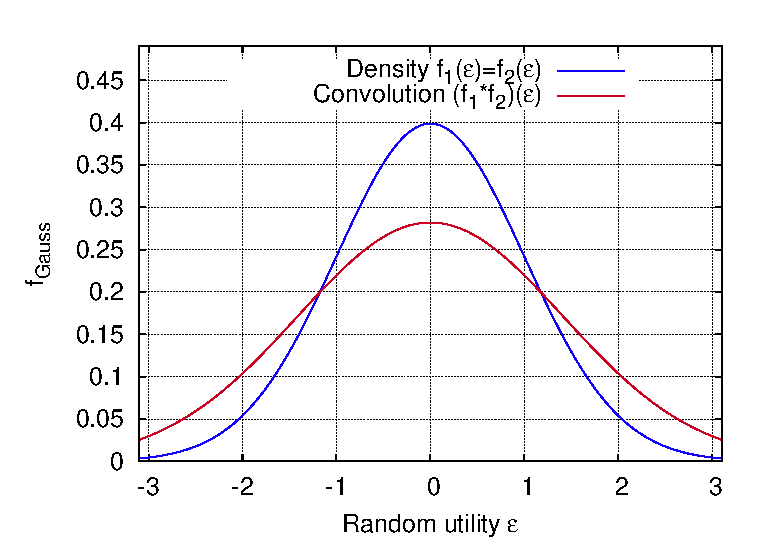
\includegraphics[width=0.5\textwidth]{./figsDiscr/fGauss.eps}   
 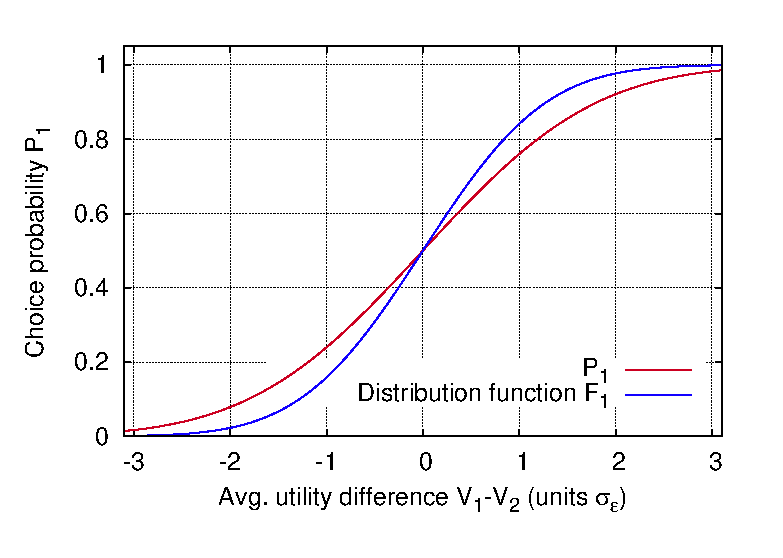
\includegraphics[width=0.5\textwidth]{./figsDiscr/binProbit_P1.eps}   
%\end{minipage}

  \caption{\label{fig:distrProbit}Probit-Modell: Links: Dichte der 
normalverteilten Zufallsnutzen $\epsilon_1$ und $\epsilon_2$ sowie die
Dichte der Nutzendifferenz $\Delta \epsilon=\epsilon_2-\epsilon_1$. Rechts:
Verteilungsfunktion der Zufallsnutzen und resultierende
Auswahlwahrscheinlichkeit f\"ur Alternative 1 in Abh\"angigkeit der
deterministischen Nutzendifferenz $V_1-V_2$.
}
\end{figure}
%###################################################

%##################################################
\subsection{Multinomiales i.i.d Probit-Modell}
%##################################################
Falls man wieder Unabh\"angigkeit der $\epsilon_i$ voraussetzt, also
nicht die allgemeinste Form der multivariaten Normalverteilung
mit nichttrivialer Kovarianzmatrix
(vgl. Abschnitt~\ref{sec:matrixGauss}), erh\"alt man aus 
\refkl{multinomAllg} folgende Auswahlwahrscheinlichkeit f\"ur
Alternative 1 ($f_1$ bezeichnet
 die Dichte der $(0,\sigeps)$-Normalverteilung):
\be
\label{multiProbit}
P_1 =\int\limits_{-\infty}^{\infty} f_1(\epsilon_1)
\Phi \left(\frac{\epsilon_1+V_1-V_2}{\sigeps}\right)
\cdots
\Phi \left(\frac{\epsilon_1+V_1-V_I}{\sigeps}\right)
\diff{\epsilon_1}.
\ee
Der Integrand besteht also aus einem Produkt von 
(kumulierten) Standardnormalverteilungen
(vgl. Abb. \ref{fig:multiProbit}).

%##################################################
\begin{figure}
 \fig{\textwidth}{./figsDiscr/pMultiProbit.eps}   
  \caption{\label{fig:multiProbit}(a) Auswahlwahrscheinlichkeit $P_1$
gem\"a\3 Gl. \protect\refkl{multiProbit} f\"ur
Alternative 1 beim
trinomialen  Probitmodell in Abh\"angigkeit der deterministischen
Nutzendifferenzen  zu (Referenz-) Alternative~3; (b) Auswahlwahrscheinlichkeit
$P_1$ im multinomialen Probitmodell als Funktion der Nutzendifferenz
$V_1-V_i$, falls alle anderen Alternativen $i$ im Mittel gleich
attraktiv sind ($V_i=V_2$ f\"ur $i\ge 2$).
}
\end{figure}
%###################################################



%#######################################
\section{\label{sec:Logit}Logit-Modelle}
%#######################################

\maintext{Logit-Modelle sind durch \text{i.i.d.} gumbelverteilte 
Zufallsnutzen
definiert.}

\noindent
Die Gumbelverteilung hat die Verteilungsfunktion
\be
\label{FGumbel}
F\sub{Gu}^{(\eta,\lambda)}(x)=\exp \left[-e^{-\lambda(x-\eta)}\right]
\ee
und die Dichtefunktion (vgl. Abb.~\ref{fig:fGumbel})
\be
\label{fGumbel}
f\sub{Gu}^{(\eta,\lambda)}(x)
=\abl{F\sub{Gu}^{(\eta,\lambda)}(x)}{x}
=\lambda e^{-\lambda(x-\eta)}
\exp \left[-e^{-\lambda(x-\eta)}\right].
\ee
%
F\"ur die Anwendung bei diskreten Wahlmodellen  wichtige Eigenschaften
der Gumbelverteilung sind die folgenden:

%##################################################
\begin{figure}
 \fig{0.5\textwidth}{./figsDiscr/gumbel_f.eps}   
  \caption{\label{fig:fGumbel}Dichten verschiedener Extremwert- bzw. Gumbelverteilungen.
}
\end{figure}
%###################################################


\bi
\item Der Lageparameter $\eta$ hat die Bedeutung des 
Modalwerts (Wert mit der h\"ochsten Dichte) und der
Skalierungsparameter $\lambda$ ist proportional zur Inversen der
Standardabweichung $\sigeps$:
\be
\label{GumbelTransl}
x\sub{modal}=\eta, \quad \sigeps=\frac{\pi}{\sqrt{6}\lambda}
\approx 1.28/\lambda \quad
\text{bzw.} \quad \lambda=\frac{\pi}{\sqrt{6}\sigeps}
\ee
Da $\eta$ die Verteilung nur verschiebt 
und $\lambda$ nur skaliert, ist
auch eine lineare Funktion $Y=a+bX$ einer $(\eta,\lambda)$-gumbelverteilten
Zufallsvariablen wieder gumbelverteilt: 
\be
\label{Gumbeli}
X \sim \text{Gu}(\eta_i,\lambda)
\ \Rightarrow \ 
a+bX \sim  \text{Gu}(a+b\eta,\lambda/b).
\ee
Da es bei den Auswahlwahrscheinlichkeiten nur auf Nutzendifferenzen
ankommt, bedeutet diese Translationsinvarianz insbesondere, dass der
Lageparameter $\eta$ keinerlei Rolle spielt (und es somit egal ist,
dass $\eta$ den Modalwert und nicht den Erwartungswert angibt).

\item Die Gumbelverteilung mit Skalierungsparameter $\lambda$ ist die Grenzverteilung des
Maximums sehr vieler unabh\"angiger stetiger Zufallsvariablen, solange
die Dichte dieser Variablen f\"ur gro\3e Werte exponentiell mit
\emph{demselben} Exponenten $\lambda$ abf\"allt\footnote{Dies
  ist neben dem Zentralen 
Grenzwertsatz (die \textit{Summe} sehr vieler beliebig verteilter
unabh\"angiger Zufallsvariablen mit endlicher Varianz ist
gau\3verteilt) ein weiteres Beispiel eines Grenzwertsatzes.} 
Deshalb hei\3t die Gumbelverteilung auch
\bfdef{\mbox{(Typ I-)} Extremwertverteilung}. 
Die Abbildung \ref{fig:gumbelGrenz1} und \ref{fig:gumbelGrenz2} zeigen
diese Grenz\-verteilungs-Eigenschaft anschaulich. F\"ur
Interessierte befindet sich die Herleitung im Abschnitt
\ref{sec:discrHerl}.

Insbesondere ist das Maximum zweier oder mehrerer unabh\"angiger 
gumbelverteilter
Zufallsgr\"o\3en \textit{gleicher Varianz} (bzw. mit identischen Skalierungsparameter
$\lambda$) wieder gumbelverteilt und zwar \emph{ebenfalls} mit unver\"anderter
Varianz bzw. 
Ska\-lierungs\-parameter $\lambda$ (Herleitung ebenfalls im Abschnitt
\ref{sec:discrHerl}): 
\be
\label{Gumbelii}
X_i \sim \text{Gu}(\eta_i,\lambda)
\ \Rightarrow \ 
Y=\max_i X_i \sim  \text{Gu} 
\left[\frac{1}{\lambda}\ln\left(\sum_{i=1}^Ie^{\lambda\eta_i}\right),\lambda \right].
\ee

Diese Eigenschaft ist auch unmittelbar einsichtig, da nach dem
vorhergehenden Satz jede
gumbelverteilte Zufallsvariable f\"ur sich das Maximum exponentiell
abfallender Verteilungen ist. Das Maximum gumbelverteilter
Variablen ist damit ebenfalls ein Maximum exponentiell
abfallender Verteilungen, also
gumbelverteilt. Insbesondere gilt bei i.i.d gumbelverteilten
Zufallsnutzen wie im Logit-Modell
\be
\label{GumbeliiHomo}
X_i \sim \text{i.i.d.} \ \text{Gu}(\eta,\lambda)
\ \Rightarrow \ 
Y=\max_i X_i \sim  \text{Gu} 
\left(\eta+ \frac{\ln I}{\lambda}, \lambda \right).
\ee

\item Schlie\3lich ist die \textit{Differenz} $Y=X_2-X_1$ zweier mit
\emph{demselben} Skalierungsparameter $\lambda$ gumbelverteilten
Gr\"o\3en logistisch verteilt:
\be
\label{Gumbeliii}
X_1 \sim \text{Gu}(\eta_1,\lambda), \ X_2 \sim \text{Gu}(\eta_2,\lambda)
\ \Rightarrow \ 
P(X_2-X_1<y)=\frac{1}{1+e^{-\lambda(y-\eta_2+\eta_1)}}.
\ee
\ei

%##################################################
\begin{figure}
 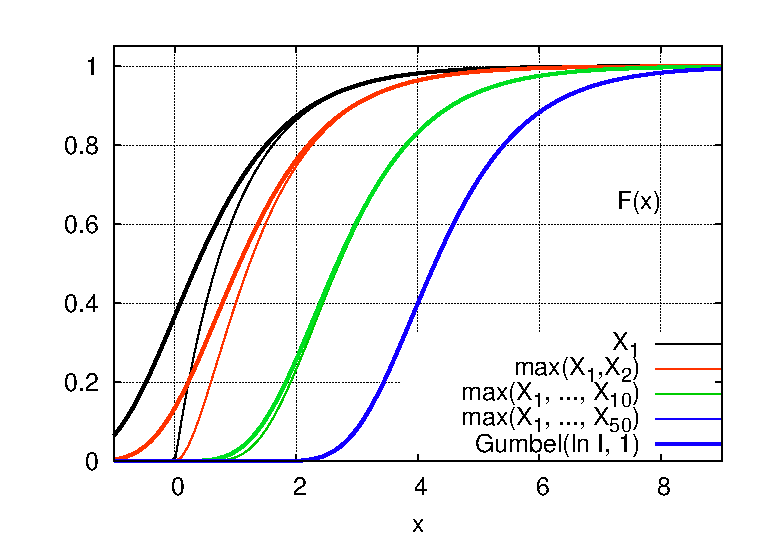
\includegraphics[width=0.5\textwidth]{./figsDiscr/gumbelGrenz_F.eps}   
 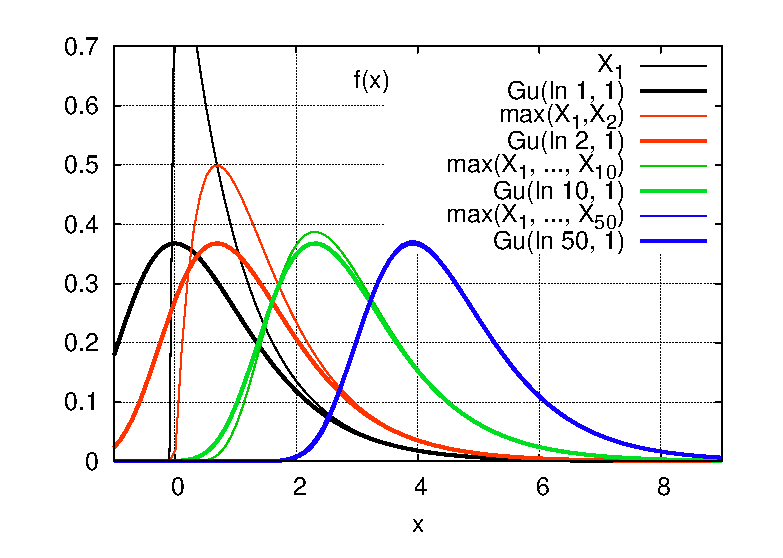
\includegraphics[width=0.5\textwidth]{./figsDiscr/gumbelGrenz_f.eps}   
  \caption{\label{fig:gumbelGrenz1}Die Gumbelverteilung als
Grenzverteilung des Maximums sehr vieler unabh\"angiger
Zufallsgr\"o\3en mit \textit{exponential tail} am Beispiel
exponentialverteilter Zufallsgr\"o\3en $X\sim E(\lambda)$ mit 
$\lambda=1$.
Geplottet ist die Verteilungsfunktion (links) und die dazugeh\"orige
Dichte (rechts) jeweils f\"ur das Maximum von $I=1,2,5,20$ und 100 
dieser Zufallsgr\"o\3en und die dazugeh\"orige
Gumbel-Grenzverteilung $Y\sim \text{Gu}(\ln I,1)$.
Bereits bei $I=20$ gibt es kaum einen sichtbaren Unterschied
zwischen der tats\"achlichen Verteilung des Maximums und der
Gumbelverteilung. 
}
\end{figure}
%###################################################


%##################################################
\begin{figure}
 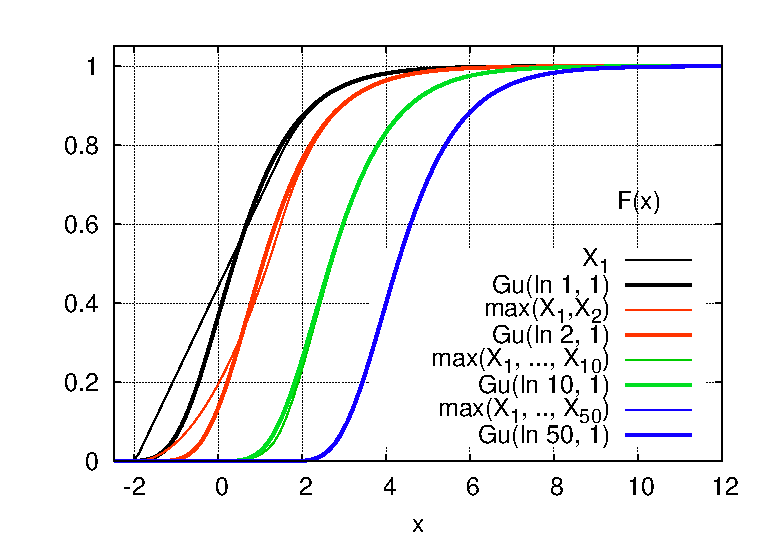
\includegraphics[width=0.5\textwidth]{./figsDiscr/gumbelGrenz2_F.eps}   
 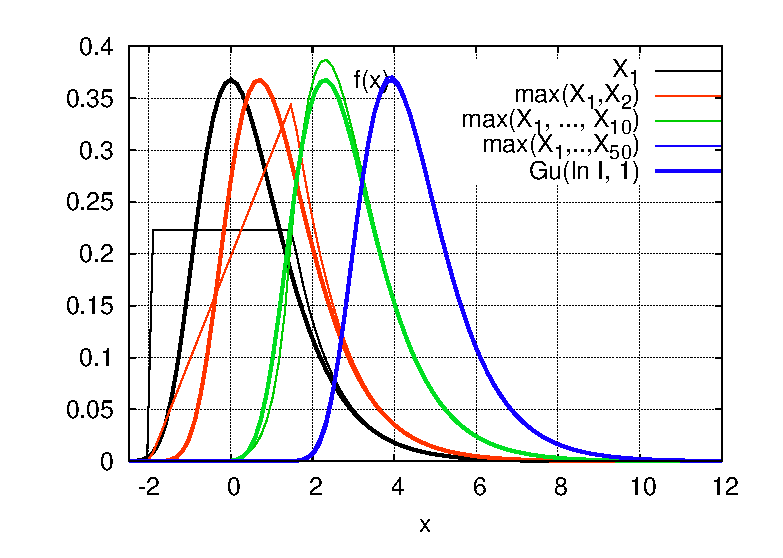
\includegraphics[width=0.5\textwidth]{./figsDiscr/gumbelGrenz2_f.eps}   
  \caption{\label{fig:gumbelGrenz2}Die Grenzverteilungseigenschaft
funktioniert auch bei anderen Verteilungen, solange ein
\textit{exponential tail} existiert. Hier ist das Maximum von
unabh\"angigen Zufallsvariablen gezeigt, welche im Interval $-1.98 \le x \le 1.5$
gleich\-verteilt sind (konstante Dichte) und erst danach exponentiell
(Exponent $\lambda=1$) abfallen. Die d\"unnen Kurven geben jeweils die
zur Zahl $I$ der exponentiell abfallenden Zufallsvariablen geh\"orige
Extremwertverteilung (Gumbelverteilung) $\text{Gu}(\ln I, 1)$
an. Wieder gibt es bereits bei $I=20$ kaum einen sichtbaren Unterschied
zwischen der tats\"achlichen Verteilung des Maximums und der
Gumbelverteilung. 
}
\end{figure}
%###################################################

%###################################################
\subsection{\label{sec:BNL}Binomiales Logit Modell}
%###################################################

Die Auswahlwahrscheinlichkeiten des Logitmodells mit zwei Alternativen
bekommt man direkt aus dem allgemeinen Ausdruck~\refkl{binAllg} mit
Hilfe der Differenz-Beziehung~\refkl{Gumbeliii} gumbelverteilter Gr\"o\3en:
\bea
\label{binLogit}
P_1\sup{BNL} &=& 
F_{\epsilon_2-\epsilon_1}(V_1-V_2)=P(\epsilon_2-\epsilon_1<V_1-V_2)
=\frac{1}{1+e^{-\lambda(V_1-V_2)}}, \\ 
P_2\sup{BNL} &=& 1-P_1\sup{BNL}. \nonumber
\eea

%###################################################
\subsection{\label{sec:MNL}Multinomiales Logit Modell}
%###################################################

Der Vorteil der Gumbel-Verteilung ist, dass man aufgrund der
Beziehungen \refkl{Gumbeliii} mit \refkl{Gumbeli} und \refkl{Gumbelii}
die Auswahlwahrscheinlichkeiten auch f\"ur beliebige Alternativenzahlen,
einfach analytisch ausdr\"ucken kann (Herleitung f\"ur Interessierte
in Abschnitt \ref{sec:discrHerl}):

%##################################################
\begin{figure}[t!]
 \fig{0.6\textwidth}{./figsDiscr/multiLogit_P1.eps}   
  \caption{\label{fig:multiLogit}Auswahlwahrscheinlichkeiten f\"ur
Alternative 1 im Multinomial-Logitmodell (dick) und 
Multinomial-Probitmodell  (d\"unn) als Funktion der deterministischen 
Nutzendifferenz $V_1-V_i$ 
dieser Alternativ zu den als gleich hoch angenommenen anderen Nutzen 
$V_i=V_2$ f\"ur $i\ge 2$. Da die Gumbelverteilung
rechtsschief ist, die Gau\3verteilung aber nicht, sind beim
Logitmodell bei vielen Alternativen
vergleichsweise h\"ohere Werte von $V_1$ n\"otig als beim Logitmodell, um dieselbe
Auswahlwahrscheinlichkeit zu erreichen.
}
\end{figure}
%###################################################

%##################################################
\begin{figure}
 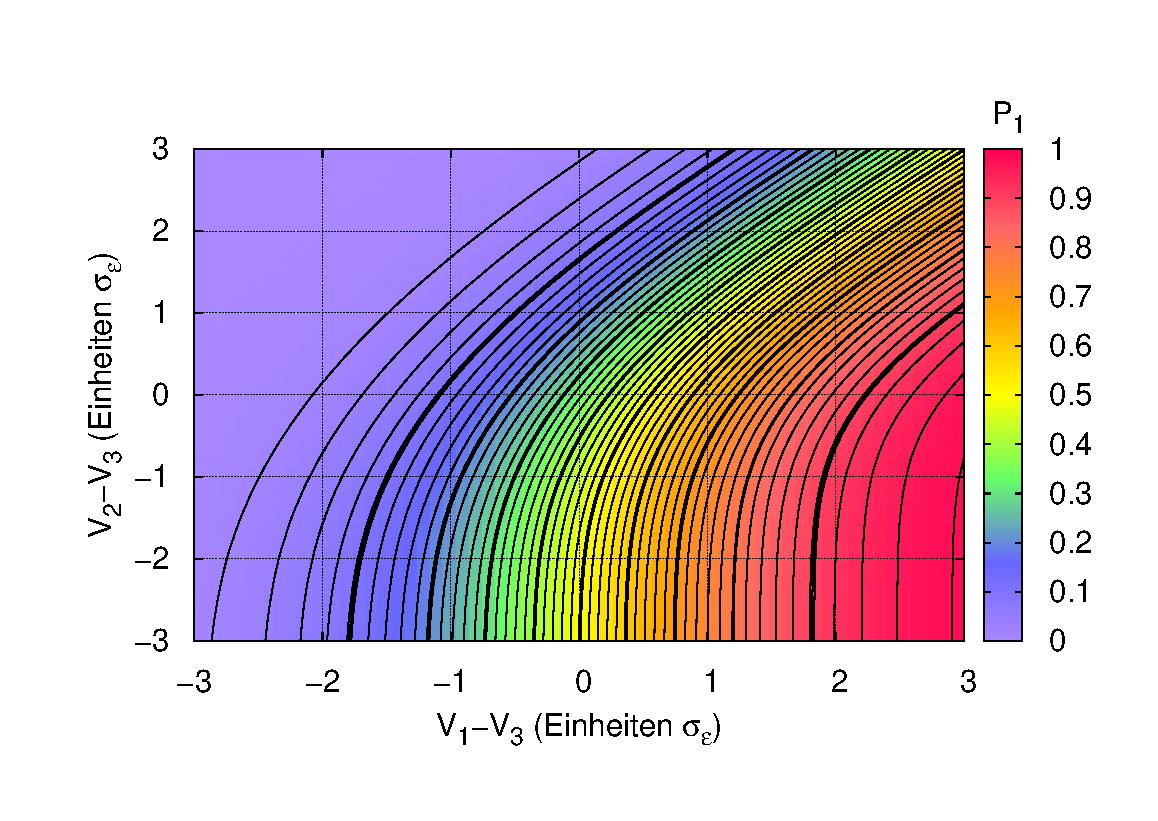
\includegraphics[width=0.5\textwidth]{./figsDiscr/p1ProbitTrinom_V1V2.eps}   
 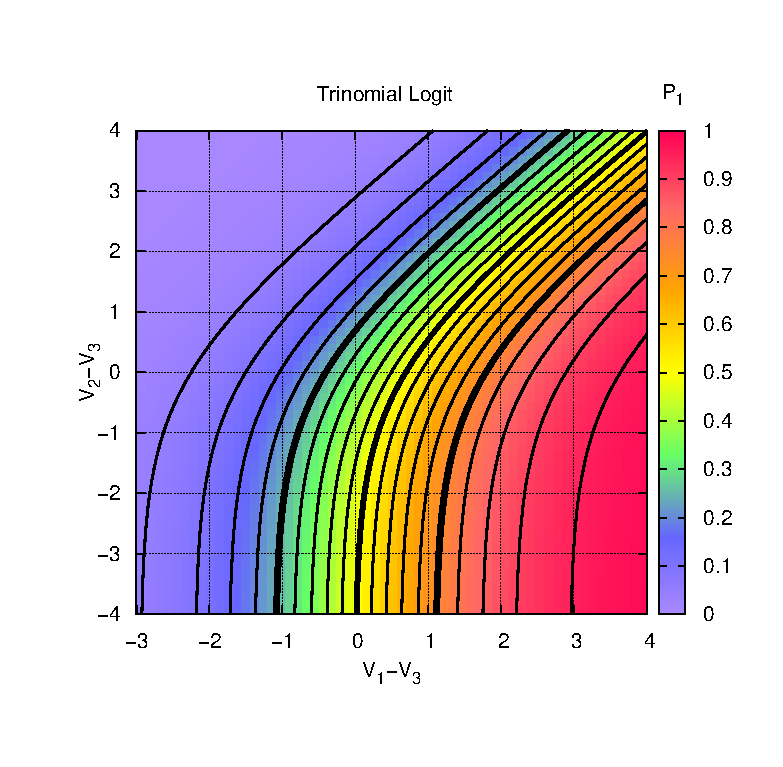
\includegraphics[width=0.5\textwidth]{./figsDiscr/pLogitTrinom_V1V2.eps}   
  \caption{\label{fig:pTrinom}Auswahlwahrscheinlichkeiten f\"ur
Alternative 1 beim trinomialen ($I=3$) Probit-Modell (links) und dem
entsprechenden Logit-Modell (rechts) in
Abh\"angigkeit der in Einheiten von $\sigeps$ skalierten Nutzenfunktionen. Ohne
Einschr\"ankung der Allgemeinheit kann der deterministische Nutzen
der Referenzalternative $V_3=0$ gesetzt werden.
}
\end{figure}
%###################################################
%
\be
\label{MNLunscaled}
P_i\sup{MNL} =\frac{e^{\lambda V_i}}{\sum\limits_{i'=1}^I e^{\lambda V_{i'}}}
=\frac{1}{\sum\limits_{i'=1}^I e^{\lambda (V_{i'}-V_i)}}
\ee
Das resultierende Multinomial-Logit-Modell (MNL)  hat folgende
wichtige Eigenschaften:
\bi
\item Es kommt (ebenso wie bei den
Probit-Modellen) nur auf die \textit{Differenzen} der deterministischen
Nutzen an. Man sagt auch, das Modell ist (ebenso wie die
Probit-Modelle) \bfdef{translationsinvariant}. Man kann also ohne
Einschr\"ankung der Allgemeinheit den Nutzen einer Alternative (z.B.
$V_1$ oder $V_I$) =0 setzen. Dies wurde bereits in
Abschnitt~\ref{sec:erh-studiBsp} ausgenutzt.

\item Die deterministischen Nutzen kommen nur als Produkt mit dem
Skalenparameter $\lambda$ bzw. in Einheiten des $\sqrt{6}/\pi$-fachen
der Zufallsnutzen-Standardabweichung vor:
\be
\label{logit-skalierung}
\lambda V_i=\frac{\pi}{\sqrt{6}} \frac{V_i}{\sigeps}
\ee
Man sagt auch, das Logit-Modell ist (ebenso wie die
Probit-Modelle) \bfdef{skaleninvariant}. Dies wurde ebenfalls bereits
in  Abschnitt~\ref{sec:erh-studiBsp} ausgenutzt.
Skaliert man den
deterministischen \emph{und} den Zufallsnutzen in  Einheit des
$\sqrt{6}/\pi$-fachen der Standardabweichung $\sigeps$ des
Zufallsnutzens, dividiert also die unskalierten Nutzenfunktionen durch
$\sigeps \sqrt{6}/\pi$, dann ist in den skalierten Gr\"o\3en der
Gumbel-Skalenparameter $\lambda=1$ und man  erh\"alt das MNL in seiner
gebr\"auchlichen standardisierten Form: 

\maineq{MNL}{
P_i\sup{MNL} =\frac{e^{V_i}}{\sum\limits_{i'=1}^I e^{V_{i'}}}
=\frac{1}{\sum\limits_{i'=1}^I e^{V_{i'}-V_i}}.
}
Zum Sch\"atzen der (in den deterministischen Nutzenfunktionen $V_i$
enthaltenen) Modellparameter $\vec{\beta}$ \emph{und} der
Standardabweichung des Zufallsnutzens kann man diese Form
verwenden (vgl. dazu 
Abschnitt~\ref{sec:nutzeninterpretation}).

\item Das MNL hat, \emph{im Gegensatz zum Probit-Modell},  die
sogenannte \bfdef{IIA-Eigen\-schaft}. Dieses K\"urzel kommt von der
englischen Bedeutung \textit{Independence of irrelevant alternatives}
und sagt aus, dass die Quotienten zweier Auswahlwahrscheinlichkeiten,
also die relative Gewichtung zweier Alternativen, \textit{nicht} von
den Nutzen irgendwelcher weiterer Alternativen abh\"angen. Dies gilt
\emph{nur} f\"ur das MNL:  Man kann sogar das Logitmodell
(und daraus die  IIA-Eigenschaft) 
nicht nur aus gumbelverteilten Zufallsnutzen herleiten, sondern
umgekehrt auch das
Logitmodell aus der
IIA-Eigenschaft:

\be
\label{IIAisMNL}
\text{I\,IA} \Longleftrightarrow \text{MNL}
\ee


\item Das MNL gilt (n\"aherungsweise) nur f\"ur exponentiell abfallende
Zufallsnutzen, also insbesondere nicht f\"ur gau\3verteilte
Zufallsnutzen, da diese quadratisch-exponentiell abfallen. 
Die im Vergleich zur Gau\3verteilung h\"oheren
Wahrscheinlichkeiten extremer Werte der Zufallsnutzen f\"uhren dazu, dass die
Wahrscheinlichkeit $P_i$ als Funktion von $V_i$ langsamer ansteigt als
beim Probitmodell (Abb. \ref{fig:multiLogit}). Genauer gesagt, ist
die Steilheit des Anstiegs von $P_i$ mit $V_i$ unabh\"angig von der
Alternativenzahl (IIA-Eigenschaft), w\"ahrend sie beim
Multi\-no\-mi\-al-Probit-Modell steiler wird. Bis zu $I=4$
Alternativen, also dem Standardfall der Verkehrsmittelwahl, sind
die Unterschiede gering (Abb.~\ref{fig:multiLogit} und~\ref{fig:pTrinom}).
\ei

%########################
\subsection{\label{sec:nutzeninterpretation}Interpretation der Parameter
     bei Probit- und Logitmodellen}
%########################
Da weder ein Hinzuf\"ugen eines konstanten Beitrags zu den
Nutzenfunktionen aller Alternativen noch eine Multiplikation der
deterministischen \emph{und} stochastischen Nutzenanteile mit einem
gemeinsamen positiven Faktor die
  Auswahlwahrscheinlichkeiten \"andern (Translations-
bzw. Skaleninvarianz)\footnote{Man kann sogar die Gesamtnutzen $U_i$
  aller Alternativen mit einer streng monoton steigenden aber sonst
  beliebig nichtlinearen Funktionen behandeln, ohne dass sich die
  Auswahlwahrscheinlichkeiten \"andern, allerdings geht dann die
  i.i.d-Eigenschaft der Zufallsnutzen verloren.}
muss man bei der Kalibrierung weder die Lage- noch die Skalenparameter
der jeweiligen Verteilung des
Zufallsnutzens sch\"atzen. Vielmehr kann beim Logitmodell $\lambda=1$
bzw. beim Probitmodell $\sigeps=1$
setzen und erh\"alt damit die standardisierten Formulierungen dieser
Modelle.
 Mit~\refkl{logit-skalierung} bedeutet dies, dass die Nutzenfunktionen
 des standardisierten Probitmodells in den Einheiten $\sigeps$ und
 die des standardisierten 
 Logitmodells in den Einheiten $(\sqrt{6}/\pi)\ \sigeps$
skaliert sind. Die Abb.~\ref{fig:multiLogit} und \ref{fig:pTrinom} zeigen, dass
 bei nicht zu gro\3er Alternativenzahl und nicht zu extremen
 Wahrscheinlichkeiten nahe null oder eins die Aussagen
der Logit- und i.i.d. Probitmodelle nahezu identisch sind, \emph{wenn
  man gleiche Nutzeneinheiten, z.B. $\sigeps$, verwendet}. Da
nach~\refkl{logit-skalierung} beim standardisierten Logitmodell
($\lambda=1$) im Vergleich zum standardisierten Probitmodell
($\sigeps=1$)  die Relation
\bdm
V\sub{Logit}=\frac{\pi}{\sqrt{6}} \frac{V}{\sigeps}
=\frac{\pi}{\sqrt{6}}V\sub{Probit}
\edm
gilt, erh\"alt man folgendes 
wichtige Ergebnis:

\maintext{Standardisierte Logitmodelle liefern weitgehend
  \"aquivalente Aussagen wie standardisierte 
bin\"are bzw. i.i.d. multinomiale Probitmodelle, wenn alle Logit-Parameter
 um den Faktor $\pi/\sqrt{6}\approx 1.28$ gr\"o\3er sind als die
 jeweiligen Probit-Parameter. Teilt man  alle
 linearen Parameter des
 standardisierten Logitmodells durch 1.28, erh\"alt man die
 deterministische Nutzenfunktion in Einheiten von $\sigeps$.} 

Dieses Ergebnis liefert letztendlich eine Begr\"undung, warum man
gumbelverteilte Zufallsnutzen annehmen kann, obwohl eine
Gau\3verteilung (aufgrund des Zentralen grenzwertsatzes) theoretisch
konsistenter ist  (vgl. den Anfang von
Abschnitt~\ref{sec:Probit}):  
Das Ergebnis ist nahezu gleich, die
Handhabung der Logitmodelle (analytische Ausrechenbarkeit, einfachere Kalibrierung) aber einfacher.

Man beachte jedoch, dass es auch deutliche Unterschiede zwischen den
beiden Modelltypen gibt, vor allem folgt aus~\refkl{IIAisMNL}, dass 
 das Probit-Modell selbst
dann nicht der IIA-Eigenschaft, wenn man i.i.d - normalverteilte
Zufallsnutzen annimmt (vgl. \"Ubungsaufgabe):
\bdm
\epsilon \sim \text{i.i.d} \ \nRightarrow \ \text{I\,IA}
\edm


\subsubsection*{Beispiel: Zwei Alternativen, Einfluss von Reisezeit und Kosten}
%
Der deterministische Nutzen zweier Alternativen $i$ sei durch
\bdm
V_{ni}=\beta_1T_{ni}+\beta_2K_{ni}+\beta_3\delta_{i1}
\edm
gegeben.  Die komplexen Reisezeiten $T_{ni}$ (in Minuten)  sowie
die Ad-Hoc-Kosten $K_{ni}$ (in \euro{}) werden also als generische
Variable formuliert. Zus\"atzlich gibt es noch einen vollst\"andigen
Satz an alternativenspezifischen Konstanten, der hier nur aus dem
Beitrag $\beta_3\delta_{i1}$ besteht. Nach getrennter Sch\"atzung der drei
Parameter im Logit- und Probitmodell sind folgende Aussagen m\"oglich:
\bi
\item Die Standardabweichung des Zufallsnutzens in
  Minuten ist durch $-1/\beta_1$ (Probitmodel)
  bzw. $-\pi/(\sqrt{6}\beta_1)$ (Logitmodell) gegeben,
\item die Standardabweichung des Zufallsnutzens in
  \euro{} ist durch $-1/\beta_2$ (Probit)
  bzw. $-\pi/(\sqrt{6}\beta_2)$ (Logit) gegeben,
\item der Zeitwert (VTTS, value of travel time savings) in \euro{} pro Minute ist gleich 
$\beta_1/\beta_2$ in beiden Modellen,
\item der globale Bonus von Alternative 1 gegen\"uber der Referenzalternative~2 in
  Nutzeneinheiten ist gleich $\beta_3$,
\item der globale Bonus von Alternative 1 gegen\"uber~2 ist gleich
  $\beta_3$ Standardabweichungen (Probit) bzw. $(\sqrt{6}/\pi)
  \beta_3$  Standardabweichungen  (Logit),
\item der globale Bonus von Alternative 1 gegen\"uber~2 in Minuten ist
  gleich $-\beta_3/\beta_1$,
\item und der globale Bonus von Alternative 1 gegen\"uber~2 in Euro
  ist gleich $-\beta_3/\beta_2$.
\ei

 
%#########################################################
\section{\label{sec:discrElast}Elastizit\"aten}
%##########################################################

Allgemein, z.B. bei Regresssionsmodellen, geben
 Elastizit\"aten die einheitenlose relative \"Anderung einer
endogenen Variable $\hat{y}_i$ als Folge einer relativer \"Anderung
einer exogenen Variablen 
$x_m$ an:
\be
\label{elast-allg}
\epsilon_i^{(m)}=\frac{x_m}{\hat{y}_i}\ablpart{\hat{y}_i}{x_m}
\ee
Falls es nur eine endogene Variable gibt, wie bei der
Regressionsrechnung, haben die Elastizit\"aten nat\"urlich nur einen
Index (bzw. Superskript), n\"amlich 
den der exogenen Variablen $x_m$. Im Gegensatz zur
Regressionsrechnung sind in der diskreten Wahltheorie die Definitionen
von Elastizit\"aten jedoch nichttrivialer und vielschichtiger. Die
verschiedenen m\"oglichen Definitionen kommen je nach Sachverhalt und
Aufgabenstellung zur Anwendung und werden an folgendem Sachverhalt
erkl\"art: 

\examplebox{Veranschaulichungs-Beispiel: Flugh\"afen}{
Gegeben sind $I$ miteinander konkurrierende
Flughafenbetreiber $i$, z.B. $i=1$: M\"unchen (MUC), 
$i=2$: Berlin (BER), $i=3$: Frankfurt (FRA) usw., welche (\"uber
entsprechende Konditionen an die 
verschiedenen Airlines) die Flugpreise eines Fluges (z.B. nach
Barcelona) f\"ur bestimmte Kundenklassen/Airlines $n$  und damit die Nachfrage
$y_{ni}$ beeinflussen k\"onnen.\footnote{Der Index $n$ bezieht sich
  dabei prim\"ar auf die Kundenklasse und (bei Auswahlm\"oglichkeit)
  auf die Airline, wodurch (\"uber den Kundenwunsch) auch indirekt das
  Flugziel fest ist. Da die Preise auch von der Flugklasse (First
  Class, Business Class, Economy) und wegen aktivem \emph{Revenue
    Management} auch vom Buchungszeitpunkt und ggf individueller
  Verg\"unstigungen abh\"angen, kann eine Kundenklasse $n$ durchaus nur
  einen einzigen Kunden ($y_{n}=\sum_iy_{ni}=1$) enthalten.} 
Wir nehmen an, dass es bei der Kundenklasse $n$ die feste Nachfrage nach 
\be
\label{defyn}
y_n=\sum_{i=1}^I y_{ni}
\ee
Fl\"ugen gibt.
F\"ur die deterministischen Nutzenfunktionen
der verschiedenen Flugh\"afen nehmen wir als Einflussfaktoren (neben den
immer notwendigen Satz von $I-1$ alternativenspezifischen Konstanten)
nur  die Gesamtkosten $K_{ni}$ und die komplexen
Reisezeiten $T_{ni}$ (von der Haust\"ur bis zum Flughafen) als
generische Variablen an:
\be
\label{Vni-Flughaefen}
V_{ni}=\beta_1K_{ni} + \beta_2 T_{ni}
+\sum_{m=1}^{I-1}\beta_{2+m}\delta_{im}.
\ee
Gesucht ist die Preiselastizit\"at der Nachfrage nach
Fl\"ugen beim Flughafen $i$, wenn Flughafen $j$ seinen Preis \"andert.
}

%##################################
\subsection{Definitionen im Rahmen der diskreten Wahltheorie}
%##################################

Obiges Beispiel zeigt, dass die Definitionsm\"oglichkeiten 
von Elastizit\"aten im Rahmen der diskreten Wahltheorie viel
reichhaltiger sind als bei den Regressionsmodellen. Dies wird durch
folgende Eigenheiten der 
Modelle der diskreten Wahltheorie verursacht:
\bi
\item sie sind \emph{mikroskopisch},
\item sie sind \emph{Mehrgleichungsmodelle}
\item und sie betreffen im Allgemeinen ein \emph{nichtteilbares Gut oder
  Dienstleistung}, was in der diskreten Skalierung der exogenen Variablen
  $y_{ni} \in \IN_0^+$ zum Ausdruck kommt.
\ei
 Wir unterscheiden drei verschiedene Kategorien, 
Elastizit\"aten zu definieren:
\benum
\item Die \bfdef{Elastizit\"at bez\"uglich Verschiebungen} bzw. die
  \bfdef{Substitutions-Elastizit\"at} 
  (engl.: \emph{mode-choice elasticity})
  gegen\-\"uber der \bfdef{vollen Elastizit\"at}
 (engl.: \emph{ordinary elasticity}). Bei der
  Verschiebungselastizit\"at ist die Entscheidung (``Flug nach
  Barcelona'') als solches gefallen und man w\"ahlt nur den Modus (das
  ``Wie'', also hier, von welchen Flughafen). Solche
  Substitutionselastizit\"aten sind vor allem bei 
  \emph{nichtteilbaren G\"utern und Dienstleistungen}, wie eben
  Fl\"ugen, relevant.
 Bei den Gesamt-Elastizit\"aten hingegen steht als
  zus\"atzliche Option ein Flugverzicht bzw. Fahrt mit Auto oder
  Bahn (\emph{no-choice} Option) zur Debatte. Ferner k\"onne auch
  bisherige Nichtflieger durch
  billigere Preise zu Barcelona-Fliegern werden. Unter einigen, oft
  allerdings nicht erf\"ullten Annahmen kann man nach \emph{Taplin}
  einen Zusammenhang zwischen diesen Elastizit\"aten finden.\footnote{David A. Hensher, Kenneth John Button,
``Handbook of transport modelling'' (2000); Oum, T.H. and Waters, WG
and Yong, J.S., ``Concepts of price elasticities of transport demand
and recent empirical estimates: an interpretative survey'', Journal of
transport economics and policy 26, 139--154 (1992).}


\item Die \bfdef{mikroskopische Elastizit\"at}, welche auf eine
  bestimmte Person und einen bestimmten Flug $n$ bezogen ist,
  gegen\"uber der \bfdef{makroskopischen 
  Elastizit\"at} bez\"uglich der gesamten Kundschaft und aller
  angebotenen Fl\"uge. Die Definition
  einer mikroskopischen Elastizit\"at wird dadurch erm\"oglicht, dass
  die Modelle der diskreten Wahltheorie mikroskopische Modelle sind,
  also \emph{auf Einzelpersonbasis}
  Auswahrscheinlichkeiten ausgeben. 


\item \bfdef{Eigenelastizit\"aten} $\epsilon_{ii}$ als
  relative \"Anderung der Nachfrage bei Flughafen $i$, wenn sich
  Flugpreise von/zu diesem Flughafen \"andern und die Preise bei allen
  anderen Flugh\"afen 
  konstant bleiben, im Gegensatz zu \bfdef{Kreuzelastizit\"aten}
  $\epsilon_{ij}$: Relative Nachfrage\"anderung bei Flughafen $i$ als Folge von
 Preis\"anderungen bei einem anderen Flughafen
  $j\neq i$. 

\eenum

\newpage

\verstaendnisbox{Welche Elastizit\"at ist betragsm\"a\3ig gr\"o\3er:
  Die Verschiebungs- oder die volle Elastizit\"at? Wie gro\3 sind
  Verschiebungs- und volle Elastizit\"aten, falls es (neben der
  No-Choice-Option) nur eine
  Wahlm\"oglichkeit ($I=1)$ gibt?}
\vspace{-1.0em}

\noindent
{\scriptsize Die volle Elastizit\"at ist betragsm\"a\3ig gr\"o\3er, da
  sie auch Entscheidungs\"anderung ``von au\3en'' bzw. ``nach au\3en''
  mit ber\"ucksichtigt. Bei $I=1$ (Monopol) ist die Verschiebungselastizit\"at =0 .}



%##################################
\subsection{\label{sec:elastMicro}Mikroskopische Preiselastizit\"aten}
%##################################

Sowohl mikroskopische Verschiebungs- als auch volle Elastizit\"aten
k\"onnen im Rahmen der Wahltheorie modelliert werden: Ordnet 
man in der Alternativenmenge der No-Choice-Option einen prohibitiv
negativen Nutzen zu, modelliert man
Verschiebungselastizit\"aten.\footnote{Erinnern Sie sich, dass die
  Alternativenmenge immer gegenseitig exklusiv und vollst\"andig sein
  muss.}
 Nimmt man jedoch f\"ur diese Option eine zu
sch\"atzenden alternativenspezifischen Konstante an, beschreibt man
die volle Elastizit\"at. 

\subsubsection*{Berechnung f\"ur das MNL bei parameterlinearen Nutzen}
Parameterlineare deterministische Nutzenfunktionen lassen sich
allgemein als Summe von $M$ exogenen Faktoren darstellen:
\be
\label{VlinAllg}
V_{ni}=\vecbeta\tr \vec{x}_{ni}=\sum_{m=1}^M \beta_m x_{nmi}.
\ee
Hierbei bezeichnet $x_{nmi}$ den $m$-ten exogenen Faktor f\"ur Person
bzw. Personengruppe $n$ und Alternative $i$.

\examplebox{Veranschaulichungs-Beispiel: Flugh\"afen}{Hier bezeichnet
  $x_{1n1}=K_{n1}$ den Flugpreis von Flughafen MUC f\"ur Person $n$,
  $x_{2n3}=T_{n3}$ die Reisezeit von der Wohnung dieser Person zum
  Flughafen FRA usw.
}


Mikroskopische Substitutionselastizit\"aten bez\"uglich des Faktors
$m$ sind allgemein definiert durch 

\maineq{elast-mic}{
\epsilon_{nij}\sup{(mic,m)}= \frac{x_{nmj}}{P_{ni}}
\ablpart{P_{ni}}{x_{nmj}}
}
oder in Worten: 
\maintext{Die mikroskopische Substitutionselastizit\"at
  $\epsilon_{nij}\sup{(mic,m)}$ bezeichnet die prozentuale \"Anderung der
  Auswahlwahrscheinlichkeit bzw. erwartete Nachfrage von Person (bzw. Personengruppe)
  $n$ f\"ur Alternative $i$, wenn
  sich der exogene Faktor $m$ der Alternative $j$ f\"ur diese
  Person um \unit[1]{\%} \"andert.
}

Die MNL-Auswahlwahrscheinlichkeit ist wie \"ublich gegeben durch
\bdm
\label{PMNLlinAllg}
P_{ni}=\frac{e^{V_{ni}}}{\sum_{k=1}^I e^{V_{nk}}}.
\edm
Ihrer partielle Ableitung nach dem jeweiligen exogenen Faktor l\"asst
sich durch Anwendung der Produkt- und Kettenregeln berechnen:
\bdma
\ablpart{P_{ni}}{x_{nmj}}
 &=& \frac{e^{V_{ni}}}{\sum_k e^{V_{nk}}}\ablpart{V_{ni}}{x_{nmj}}
  - \frac{e^{V_{ni}}}{\left(\sum_k e^{V_{nk}}\right)^2}
    \ablpart{}{x_{nmj}}\left(\sum_k e^{V_{nk}}\right) \\
 &=& P_{ni}\ablpart{V_{ni}}{x_{nmj}}
  - \sum_k \frac{e^{V_{ni}}e^{V_{nk}} }{\left(\sum_k e^{V_{nk}}\right)^2}
    \ablpart{V_{nk}}{x_{nmj}} \\
 &=& P_{ni}\left(\ablpart{V_{ni}}{x_{nmj}}
  - \sum_k P_{nk} \ablpart{V_{nk}}{x_{nmj}}\right).
\edma
Mit~\refkl{VlinAllg} ergeben sich die partiellen Ableitungen zu
\bdm
\ablpart{V_{ni}}{x_{nmj}}=\beta_m\delta_{ij}=\beta_m\twoCases{1}{i=j}{0}{\text{sonst,}}
\qquad
\ablpart{V_{nk}}{x_{nmj}}=\beta_m\delta_{kj}
\edm
und damit
\be
\label{ablPni-xmnj}
\ablpart{P_{ni}}{x_{nmj}}=\beta_mP_{ni}\left(\delta_{ij}-P_{nj}\right).
\ee
Mit der Definition~\refkl{elast-mic} sind die mikroskopischen
Elastizit\"aten des MNL bei parameterlinearen 
deterministischen Nutzenfunktionen schlie\3lich gegeben
durch
\maineq{elast-mic-MNL}{
\epsilon_{nij}\sup{(mic,m)}=\beta_mx_{nmj}\left(\delta_{ij}-P_{nj}\right).
}
Damit ergeben sich
\bi
\item die mikroskopischen Eigenelastizit\"aten
\be
\epsilon_{nii}\sup{(mic,m)}=\beta_mx_{nmi}\left(1-P_{ni}\right),
\ee
\item die mikroskopischen Kreuzelastizit\"aten:
\be
\epsilon_{nij}\sup{(mic,m)}=-\beta_mx_{nmj}P_{nj}.
\ee
\ei
Aufgrund der IIA-Eigenschaft h\"angen die Kreuzelastizit\"aten
\emph{nicht} vom Ziel $i$ ab, d.h. alle Alternativen $i$ sind
gleicherma\3en von einer \"Anderung der Attribute von $j$ betroffen. 

\aufgabenbox{Aufgabe: Substitutionselastizit\"at beschreibt
  Nullsummenspiel}{
Zeigen Sie, dass allgemein folgende Summenbedingung gilt:
\bdm
\sum_i P_{ni}\epsilon_{nij}\sup{(mic,m)}=0,
\edm
indem Sie beispielsweise $j=1$ setzen (bei Alternative $1$ wird das
Attribut $m$ ge\"andert). Zeigen Sie, dass hinter dieser Beziehung
nichts anderes als ein Nullsummenspiel steht: Was einer gewinnt, wird
dem bzw. den anderen genommen.
}
 
\examplebox{Veranschaulichungs-Beispiel: Flugh\"afen}{
Bei den deterministischen Nutzenfunktionen der Flugh\"afen,
Gl.~\refkl{Vni-Flughaefen}, haben die Preiselastizit\"aten folgende Bedeutung:

\bi
\item Erh\"oht sich der Preis an Flughafen $i$ um \unit[1]{\%}, dann
  erh\"oht sich die Wahrscheinlichkeit f\"ur Person $n$, diesen
  Flughafen zu w\"ahlen, um 
 $\epsilon_{nii}\sup{(mic,K)}=\beta_1K_{ni}\left(1-P_{ni}\right)$
  Prozent. Da die Preissensitivit\"at $\beta_1<0$ und $1-P_{ni}>0$ sind,
  wird die Wahrscheinlichkeit bei Erh\"ohung des Preises
  \emph{reduziert}.

\item Erh\"oht sich der Preis an Flughafen $j$ um \unit[1]{\%}, dann
  erh\"oht sich die Wahrscheinlichkeit f\"ur Person $n$, Flughafen
  $i\neq j$ zu w\"ahlen, um 
$\epsilon_{nij}\sup{(mic,K)}=-\beta_1K_{nj}P_{nj}$ Prozent. Da die
  Preise und Wahrscheinlichkeiten positiv sind und $\beta_1<0$ ist,
  f\"uhrt eine Preiserh\"ohung bei Flughafen $j$ zu einer 
  prozentualen \emph{Zunahme} der Wahl aller Flugh\"afen $i \neq
  j$. Alle Konkurrenzflugh\"afen $i$ erhalten dabei die gleiche
  relative Nachfragesteigerung. 
\ei
}

%##################################
\subsection{\label{sec:elastMacro}Makroskopische Preiselastizit\"aten}
%##################################

Zun\"achst ist die makroskopische
  Elastizit\"at weder gleich der mit dem Wahlmodell wie
  oben berechnete Elastizit\"at f\"ur mittlere exogene Faktoren
  $\bar{x}_{mi}=1/N\sum_n x_{nmi}$ noch ist sie ein direkter Mittelwert der
  mikroskopischen Elastizit\"aten. Vielmehr muss man bei der
  Aggregierung die pers\"onlichen Einflussfaktoren und
  Wahlwahrscheinlichkeiten individuell betrachten. 

Allgemein ist die makroskopische Elastizit\"at bez\"uglich des Faktors
$m$ definiert durch
\be
\label{elast-mac}
\epsilon_{ij}\sup{(mac,m)}=\frac{X_{mj}}{N_i}\ablpart{N_i}{X_{mj}}.
\ee
Die makroskopischen Merkmalssummen\"o\3en (gekennzeichnet durch Gro\3buchstaben)
bedeuten:
\bi
\item $N_i=\sum_nP_{ni}$ die vom Modell
  gesch\"atzte Wahlh\"aufigkeit f\"ur Alternative $i$,
\item $X_{mj}=\sum_nx_{nmj}$ die potenzielle (maximale)
  Merkmalssumme des Merkmals bzw. Faktors  $m$ bei Alternative $j$,
  wenn alle diese Alternative w\"ahlen, bzw. der Mittelwert $1/N
  \sum_nx_{nmj}$ des exogenen Faktors \"uber alle Personen (der Unterschied
  k\"urzt sich bei der Definition~\refkl{elast-mac} heraus), 
\item $\ablpart{N_i}{X_{mj}}$ die \"Anderung der Wahlh\"aufigkeit der Alternative
  $i$ bei \"Anderung des Mittelwertes des Faktors $m$ der
  Alternative $j$.
\ei
In Worten:
\maintext{Die makroskopische Substitutionselastizit\"at
  $\epsilon_{ij}\sup{(mac,m)}$  bezeichnet die prozentuale \"Anderung der
  Wahlh\"aufigkeit bzw. Nachfrage $N_i$ f\"ur Alternative $i$, wenn sich bei Alternative
  $j$ der \"uber alle Personen gemittelte exogene Faktor $m$  um \unit[1]{\%}
  \"andert. Ist $m$ beispielsweise der Preis, gibt
  $\epsilon_{ij}\sup{(mac,m)}$ die prozentuale Erh\"ohung der
  Gesamtnachfrage nach $i$ an, wenn sich die Preise bei $j$ im Mittel um
  \unit[1]{\%} erh\"ohen.
}
Diese Definition ist jedoch nicht eindeutig, da sie offen l\"asst, wie
sich die \"Anderungen der Merkmalssumme auf die einzelnen Personen
aufteilt. Es gibt zwei offensichtliche
Aufteilungsm\"oglichkeiten:
\bi
\item \textbf{Absolute \"Anderungen} um einen festen Betrag:
\be
\label{auftAbs}
\diff{x_{nmj}}=\diff{X_{mj}}
\ee
Hier \"andern sich die Attribute bei allen Personen $n=1, \ldots, N$ um denselben
\emph{absoluten} Betrag, welcher nat\"urlich dann gleich der \"Anderung $\diff{X_{mj}}$
des Mittelwertes ist.
ist.  
\item \textbf{Relative \"Anderungen:}
\be
\label{auftRel}
\frac{\diff{x_{nmj}}}{x_{nmj}}=\frac{\diff{X_{mj}}}{X_{mj}}
\ee
Hier \"andern sich die Attribute bei allen Personen um denselben
\emph{relativen} Betrag, welcher dann nat\"urlich gleich der relativen
\"Anderung des Mittelwertes \"uber alle Personen ist.
\ei

\subsubsection*{Formulierung als Funktion der mikroskopischen Elastizit\"aten}
Bei den \textbf{absolute \"Anderungen} gilt mit der Definition~\refkl{elast-mic} der
makroskopischen Elastizit\"at  sowie der Aufteilungsregel~\refkl{auftAbs}
\bdm
\ablpart{N_i}{X_{mj}}=\sum_n\ablpart{P_{ni}}{X_{mj}}
=\sum_n\ablpart{P_{ni}}{x_{nmj}}=\sum_n\frac{P_{ni}}{x_{nmj}}\epsilon_{nij}\sup{(mic,m)}
\edm
und damit mit der Definition~\refkl{elast-mac} der
makroskopischen Elastizit\"at:
\be
\label{elast-mac-abs}
\epsilon_{ij}\sup{(mac,abs,m)}=\frac{X_{mj}}{N_i}\ablpart{N_i}{X_{mj}}
= \frac{X_{mj}}{N_i}\sum_n\frac{P_{ni}}{x_{nmj}}\epsilon_{nij}\sup{(mic,m)}.
\ee
%
Bei den \textbf{relativen \"Anderungen} verwendet man hingegen die
Aufteilungsregel~\refkl{auftRel} und erh\"alt
\bdm
\ablpart{N_i}{X_{mj}}=\sum_n\ablpart{P_{ni}}{X_{mj}}
=\sum_n\frac{x_{nmi}}{X_{mj}}\ablpart{P_{ni}}{x_{nmj}}
=\sum_n\frac{P_{ni}}{X_{mj}}\epsilon_{nij}\sup{(mic,m)}
\edm
%
und damit wieder mit der Definition~\refkl{elast-mac}:
\be
\label{elast-mac-rel}
\epsilon_{ij}\sup{(mac,rel,m)}
=\frac{1}{N_i}\sum_n P_{ni}\epsilon_{nij}\sup{(mic,m)}.
\ee

Mit der Gewichtung 
\bdm
w_{ni}=\frac{P_{ni}}{N_i}=\frac{P_{ni}}{\sum_n P_{ni}}
\edm
kann man dies auch schreiben als
\be
\epsilon_{ij}\sup{(mac,rel,m)}=\sum_n w_{ni}\epsilon_{nij}\sup{(mic,m)}.
\ee
Dies ist ein gewichtetes Mittel der relativen Elastizit\"aten, wobei
die Gewichtung proportional des erwarteten Anteils der Person $n$ an der
(bisherigen) Gesamtnachfrage $N_i$   f\"ur Alternative $i$ ist.


\examplebox{Veranschaulichungs-Beispiel: Flugh\"afen}{
\bi
\item Die Elastizit\"at $\epsilon_{ij}\sup{(mac,abs,1)}$ bezeichnet die
prozentuale \"Anderung der Gesamtnachfrage an Fl\"ugen von Flughafen $i$,
wenn Flughafen $j$ den Preis (=Faktor bzw. Attribut~1) 
f\"ur alle Fl\"uge um einen gleichen
festen Betrag \"andert, so dass sich der Gesamtpreis aller
angebotenen Fl\"uge um  \unit[1]{\%} \"andert. 

\item Die Elastizit\"at $\epsilon_{ij}\sup{(mac,rel,1)}$ bezeichnet die
prozentuale \"Anderung der Gesamtnachfrage an Flughafen $i$, wenn
Flughafen $j$ auf alle Preise \unit[1]{\%} aufschl\"agt. Diese
Elastizit\"at ist gleich dem gewichteten
Mittel der mikroskopischen Elastizit\"aten, wobei die Wichtung gleich
dem erwarteten Anteil des Fluggastes $n$ an der Gesamtnachfrage  des Flughafens $i$ ist.
\ei
}


\subsection{Exkurs: Revenue Management}
\red{\texttt{Siehe README\_RevenueManagementNeuBringen\_14}}


%########################
\section{\label{sec:maxlikelihood}Einschub: Die Maximum-Likelihood-Methode} 
%########################

Zur Parametersch\"atzung bzw. Modellkalibrierung kam bei 
Regressionsmodellen die Least-Squares-Errors (LSE)
Methode zum Einsatz. Diese ist jedoch bei den Modellen der diskreten
Wahltheorie nicht immer wohl definiert, geschweige denn, dass sie zu
unverzerrten oder gar effizienten Sch\"atzern f\"uhrt. Das Problem
ist die Definition der Fehlerquadratsumme: Da die Wahltheorie-Modelle,
im Gegensatz zu den Regressionsmodellen,
 Wahrscheinlichkeitsaussagen machen (bei den Regressionsmodellen ist
$\epsilon$ ja nur der nichtmodellierte Restanteil), ist eine direkte
Bildung der Art ``Summe der quadrierten Abweichungen zwischen
modellierten und beobachteten Wert'' nicht m\"oglich. Allenfalls
k\"onnte man versuchen, die modellierten Wahrscheinlichkeiten mit den
beobachteten relativen H\"aufigkeiten m\"oglichst gut in \"Ubereinklang
zu bringen. Das f\"uhrt jedoch im Allgemeinen nicht auf effiziente
oder selbst unverzerrte Sch\"atzer.\footnote{Die
  Kalibrierungsbedingungen~\refkl{kalibMNL}
 des Logitmodells k\"onnte man jedoch so interpretieren.} 

Gl\"ucklicherweise gibt es zum Sch\"atzen von Wahlmodellen ein
alternatives Verfahren, die \bfdef{Maximum-Likelihood-Methode}.
Bei dieser, oft auch als ML abgek\"urzte Methode
 werden die Beobachtungen
\be
\label{Yni}
y_{ni}=\twoCases{1}{\text{Person $n$ hat Alternative $i$ gew\"ahlt}}{0}{\text{sonst,}}
\ee
also die endogenen Variablen,
als Realisierungen des stochastischen
Modells gesehen, welches durch die Alternativenzahl 
definiert ist: Dabei  betrachten wir den Fall, dass
jede Person $n$ nur genau eine Alternative w\"ahlen
kann,\footnote{Falls es f\"ur eine Person mehrere Wahl-Situationen
  gibt, oder eine homogene 
  Personengruppe, welche als eine Einheit
  betrachtet wird, wiederholt man die Wahlentscheiding entsprehend
  h\"aufig. Man geht also in der Modellierung, zumindest konzeptionell, auf 
jedem Fall mikroskopisch vor.}
 also
\be
\label{sumruley}
y_n=\sum_{i=1}^Iy_{ni}=1.
\ee
Bei gegebenen Auswahlwahrscheinlichkeiten $P_{ni}$ ergibt das im Modell
bei  zwei Alternativen die $(1,P_{n1})$ - Binomialverteilung. Der erste
Parameter besagt, dass es sich nur um eine Ja-Nein-Entscheidung
(\emph{Bernouilli-Experiment}) handelt, w\"ahrend der zweite Parameter
die Wahrscheinlichkeit f\"ur die Wahl der Alternative~1 (``ja'')
angibt. Bei mehr als zwei
Alternativen verallgemeinert man die Binomialverteilung 
 durch eine durch eine durch die Wahrscheinlichkeiten
 $P_{n1}, ..., P_{n,I-1}$ charakterisierte 
\emph{Multinomial\-verteilung}.\footnote{Wegen $\sum_iP_{ni}=1$ ist
  jeweils die letzte Wahrscheinlichkeit $P_{nI}$ der Binomial- und
  Multinomialverteilung nicht unabh\"angig und deshalb kein
  Parameter.} 
Falls, wie hier, nur jeweils eine Entscheidung
betrachtet wird ($\sum_i y_{ni}=1$), ergeben sowohl die Binomial- als
auch die  Multinomial\-verteilung mit der Wahrscheinlichkeit
$P_{ni_n}(\vecbeta)$ den 
``richtigen'' Vektor
\bdm
\vec{y}_n=(0,...,0,1,0,..0)\tr,
\edm
wobei die 1 an der Position $i_n$ der tats\"achlich bei Wahl $n$ gew\"ahlten
Alternative steht (vgl. Gl.~\refkl{multinom} im n\"achsten Abschnitt).


Nun wird, in Abh\"angigkeit des Parametervekktors
$\vec{\beta}$, die kombinierte Wahrscheinlichkeit daf\"ur berechnet, dass
die Messung 1 den Wert $\vec{y}_1$, \ldots, die Messung $N$ den Wert $\vec{y}_N$
liefert:
\be
\label{ML-allg}
L(\vec{\beta})
=\text{Prob}(\vec{Y}\!_1(\vecbeta)=\vec{y}_1, \vec{Y}\!_2(\vecbeta)=\vec{y}_2, \ldots,
\vec{Y}\!_N(\vecbeta)=\vec{y}_N) = \text{max}(\vecbeta). 
\ee
Bei festen Messdaten, aber in  Abh\"angigkeit der Parameter, wird
diese Funktion \bfdef{Likelihoodfunktion} genannt.\footnote{Im
  Englischen wird unterschieden zwischen \emph{probability}
  (Wahrscheinlichkeit, 
  dass eine Zufallsgr\"o\3e mit fester Verteilung, also festen
  Parametern, einen bestimmten Wert liefert) und
  \emph{Likelihood} (Wahrscheinlichkeit, mit der in Abh\"angigkeit der
  Parameter eine Zufallsgr\"o\3e einen vorgegebenen Messwert
  trifft). Insbesondere ist bei diskreten Zufallsgr\"o\3en die 
  Wahrscheinlichkeitsfunktion diskret, w\"ahrend die
  \emph{Likelihoodfunktion} immer kontinuierlich ist: Im Gegensatz zu den
  exogenen oder endogenen Variablen werden die Modellparameter
  n\"amlich immer kontinuierlich angenommen.}
 Die im Parametervektor $\vec{\beta}$ enthaltenen Parameter
werden so bestimmt, dass die
\emph{Likelihood}, also die 
Wahrscheinlichkeit daf\"ur, dass das stochastische Modell die Messungen
liefert, maximal ist.

Die Anwendungsgebiete der LSE und der ML-Methode \"uberschneiden sich,
da man letztere auch auf stetige endogene Variable anwenden 
kann.\footnote{Bei stetigen Gr\"o\3en ist die
Wahrscheinlichkeit des Eintreffens eines festen Wertes 
i. A. exakt gleich Null. Deshalb wird in diesem Fall, genau genommen, die
\emph{Wahrscheinlichkeitsdichte} maximiert. Die ML-Sch\"atzer
entsprechen also 
der Stelle, bei welcher die Dichte der kombinierten
Wahrscheinlichkeitsfunktion an der Stelle der gemessenen endogenen
Variablen bez\"uglich der Parameter maximal ist. Bez\"uglich der
Parameter, also als Likelihoodfunktion, ist die Verteilung aber in
beiden F\"allen stetig, so dass eine Unterscheidung nicht n\"otig ist.}
Es gilt:
\bi
\item Die LSE-Methode kann man bei stetigen endogenen Variablen und
beliebiger, auch nicht explizit vorgegebener, Verteilung der
Zufallsgr\"o\3en anwenden.
\item Die ML-Methode kann man bei stetigen und diskreten endogenen
Variablen anwenden, aber die Form der Verteilung der Zufallsgr\"o\3en
muss explizit gegeben sein.
\ei

%#########################################################
\subsection{Regressionsmodelle: Vergleich mit der LSE-Methode}
%#########################################################

Als erstes Beispiel wenden wir die ML-Methode auf das vollst\"andig
nach Gau\3-Markow spezifizierte lineare
multivariate Regressionsmodell~\refkl{oekonLin} an.\footnote{In diesem
  Beispiel wird wieder die Indexkonvention der Regressionsrechnung
  verwendet, also $i$ f\"ur den $i$-ten Satz an Messwerten
  $(\vec{x}_i,y_i)$.}
Das Modell lautet also
\bdm
Y(\vec{x}; \vecbeta)=\sum_{m=0}^M\beta_mx_m+\epsilon=\vecbeta \vec{x}+\epsilon, \quad \epsilon 
\sim N(0,\sigeps^2)
\edm
und die dazugeh\"origen Systemgleichungen
\bdm
\vec{Y}=\m{X}\vecbeta+\vec{\epsilon}, \quad \text{mit} \quad 
\veceps=(\epsilon_1, ..., \epsilon_i, ..., \epsilon_n)\tr, \quad
\epsilon_i \sim \text{i.i.d}\ N(0,\sigeps^2).
\edm
Die Wahrscheinlichkeit, dass das Modell die Messung $i$ beschreibt, oder
genauer, die Wahrscheinlichkeitsdichte des Modells mit den exogenen
Variablenvektor $\vec{x}_i$ an der Stelle $y_i$
lautet
\bdm
f_i(y_i)=\frac{1}{\sqrt{2\pi\sigeps^2}}
\exp\left[-\frac{(y_i-\vec{\beta}\vec{x}_i)^2}{2\sigeps^2}\right].
\edm
Da die Zufallsgr\"o\3e $\epsilon_i$ der Messung $i$ von den
Zufallsgr\"o\3en anderer
Messungen  unabh\"angig ist (i.i.d-Eigenschaft), ist die
Likelihooddichte des verbundenen Ereignisses, dass dass
Modell \emph{alle} Messungen $y_i$, $i=1, ..., n$ beschreibt, durch das
Produkt gegeben:
\be
L(\vec{\beta})=\prod_{i=1}^nf_i(y_i)
 = \prod_{i=1}^n\frac{1}{\sqrt{2\pi\sigeps^2}}
\exp\left[-\frac{(y_i-\vec{\beta}\vec{x}_i)^2}{2\sigeps^2}\right].
\ee
Das Rechnen und Ableiten mit Produkten ist umst\"andlich. Deshalb
ber\"ucksichtigt man, dass sich die Stelle $\hatvecbeta$, an der die
Likelihood-Dichte ihr Maximum aufweist, durch Anwenden einer streng
monoton steigenden Funktion auf $L$ nicht \"andert. Insbesondere ist der
Logarithmus eine solche Funktion und er erweist sich als g\"unstig, da er
Produkte in Summen umwandelt. Dies ergibt hier die
\bfdef{Log-Likelihood}(dichte)
\bea
\label{lin-loglikelihooddens}
\tilL(\vec{\beta}) &=&\ln L(\vec{\beta}) \nonumber\\
 &=& \sum_{i=1}^n\left\{
 -\frac{1}{2}(\ln 2\pi+\ln \sigeps^2)
 -\left[\frac{(y_i-\vec{\beta}\vec{x}_i)^2}{2\sigeps^2}\right]\right\}
 \nonumber\\
 &=& -\frac{n}{2}(\ln 2\pi+\ln \sigeps^2)
 -\frac{1}{2\sigeps^2}(\vec{y}-\m{X}\vec{\beta})\tr(\vec{y}-\m{X}\vec{\beta}).
\eea
Wie der Name schon sagt, maximiert man bei der ML-Methode die
\emph{Likelihood}. Als notwendige (und hier hinreichende) Bedingungen
muss der Gradient, d.h. alle partiellen Ableitungen, verschwinden. Mit
den  Ableitungsregeln in Kap.~\ref{sec:matrixRules} ergibt dies
\be
\label{hatvecbetaML}
\ablpart{\tilL}{\vec{\beta}}=\frac{1}{2\sigeps^2}
(2\m{X}\tr\vec{y}-2\m{X}\tr\m{X}\vec{\beta})\stackrel{!}{=} 0
\quad \Rightarrow \quad 
\hatvecbeta=(\m{X}\tr\m{X})^{-1}\m{X}\tr\vec{y}
\ee
Man erh\"alt also dasselbe Ergebnis wie bei der LSE-Methode!
Ableiten nach $\sigeps^2$ (nicht nach $\sigeps$) liefert
\bdm
\ablpart{\tilL}{\sigeps^2}=-\frac{n}{2\sigeps^2}+\frac{1}{2\sigeps^4}
 (\vec{y}-\m{X}\vec{\beta})\tr(\vec{y}-\m{X}\vec{\beta})
 \stackrel{!}{=} 0
\edm
und daraus
\bdm
\sigeps^2=\frac{(\vec{y}-\m{X}\vec{\beta})\tr(\vec{y}-\m{X}\vec{\beta})}{n}
 = \frac{S}{n}
\edm
mit der LSE-Fehlerquadratsumme $S$.
Setzt man~\refkl{hatvecbetaML} ein, erh\"alt man
\be
\hatsigeps^2=\frac{S\sub{min}}{n}.
\ee
Dies ist jedoch \emph{kein} unverzerrter Sch\"atzer  der Residualvarianz, da dieser
nach~\refkl{linMulti_resVar} $(n-M-1)$ und nicht $n$ im Nenner
hat. Der Sch\"atzer $\hatvecbeta$ selbst ist jedoch unverzerrt (erwartungstreu), da
identisch mit dem der LSE-Sch\"atzung.
Wir halten fest:

\maintext{Beim linearen oder quasilinearen Modell mit i.i.d. gau\3verteilten
St\"orgr\"o\3en $\epsilon$ liefert die ML-Methode f\"ur die Parameter
$\vec{\beta}$ exakt denselben Sch\"atzer wie die LSE-Methode. Der
ML-Sch\"atzer der Residualvarianz ist jedoch verzerrt (aber immerhin konsistent).}

Schlie\3lich wird noch begr\"undet, warum die Dichte der mehrdimensionalen
Gau\3\-ver\-tei\-lung \refkl{betaDensity} der Schwankungen der
Parametersch\"atzer auch ``Likelihood-Dichte'' genannt wird:
Spaltet man $\vec{\beta}$ in den Sch\"atzer $\hatvecbeta$ und der
Abweichung $\Delta \hatvecbeta=\vecbeta-\hatvecbeta$ des wahren Wertes vom Sch\"atzer auf
und setzt dies in die Log-Likelihood-Dichte~\refkl{lin-loglikelihooddens}
ein, so ergibt sich 
\bdm
\tilL(\Delta\hatvecbeta)=\text{const.}
 - \frac{1}{2\sigeps^2}
\left[\vec{y}^2-\vec{y}\m{X}(\hatvecbeta+\Delta \hatvecbeta)
 - (\hatvecbeta\tr+\Delta \hatvecbeta\tr)\m{X}\tr\vec{y}
+ (\hatvecbeta\tr+\Delta \hatvecbeta\tr)\m{X}\tr\m{X}
  (\hatvecbeta+\Delta \hatvecbeta)\right]
\edm
Nach geschicktem Umformen unter Verwendung von 
$\hatvecbeta=(\m{X}\tr\m{X})^{-1}\m{X}\tr\vec{y}$ ergibt sich
\be
\label{tilLquadratForm}
\tilL(\Delta\hatvecbeta)=\text{const.}
 - \frac{1}{2\sigeps^2} \Delta \hatvecbeta\tr\m{X}\tr\m{X}\Delta \hatvecbeta
\ee
Dies ist genau der Logarithmus von~\refkl{betaDensity}!
Damit ist die Bezeichnung ``Likelihood-Dichte''
f\"ur die multivariate Dichtefunktion der Parametersch\"atzer
gerechtfertigt. \emph{Ein- und dieselbe Verteilung} bezeichnet also sowohl
die Schwankungen der Sch\"atzer um den wahren Wert, als auch (mit
anderer Normierung) die
Wahrscheinlichkeitsdichte (bez\"uglich des Parametervektors) 
daf\"ur, dass das Modell mit den
gesch\"atzten Parametern die Daten erkl\"aren kann!

%#########################################################
\subsection{\label{sec:discrKalibTrivial}Anwendung auf das einfachste Wahlmodell}
%#########################################################

Ehe im n\"achsten Abschnitt die eigentlichen Modelle der diskreten
Wahltheorie mit der ML-Methode gesch\"atzt werden, erfolgt nun ``zum
Kennenlernen'' eine Anwendung auf das wohl einfachstm\"ogliche Modell
diskreter Entscheidungen: $N$ Personen antworten unabh\"angig
voneinander eine Ja-Nein Frage. Ordnet man der Antwort ``Ja'' die
Alternative~1 und ``Nein'' Alternative~2 zu, ergeben sich $N_1=\sum_n y_{n1} \le N$
Ja-Antworten. Wie das ``Trivialmodell'' der linearen Regression hat 
das Modell keine exogenen Variablen, d.h., alle 
befragten Personen kommen aus einer verhaltenshomogenen Gruppe. Damit
gilt $P_{n1}=P_1$ f\"ur alle Personen $n$ und wir k\"onnen 
anstelle eines expliziten Wahlmodells direkt die
$(1,P_1)$-Binomialverteilung als ``Modell'' heranziehen. Dieses
Modell liefert f\"ur jede befragte Person die endogene Variable $y_{n1}$ (0:
``nein''; 1: ``ja''):
\be
Y_{ni}=\twoCases{1}{\text{mit Wahrscheinlichkeit $P_1$}}{0}{\text{sonst.}}
\ee
%
Da genau eine Alternative gew\"ahlt wird, ist $Y_{n2}=1-Y_{n1}$
abh\"angig und braucht nicht separat betrachtet werden: Wenn die
Beobachtung $y_{n1}$
richtig vorausgesagt wurde, dann auch $y_{n2}$.
Die Anwendung des Modells auf $N$ Personen liefert f\"ur die
Gesamtzahl  $N_1=\sum_n y_{n1}$ an Ja-Antworten die 
$(N,P_1)$-Binomialverteilung, da eine Summe von unabh\"angigen
$(1,P_1)$ binomialverteilten Zufallsgr\"o\3en $(N,P_1)$
binomialverteilt ist. Damit 
ergibt sich folgende Likelihoodfunktion:
\bdm
L(P_1) = \ueber{N}{N_1} P_1^{N_1}(1-P_1)^{N-N_1} 
\edm
und damit die Log-Likelihood
\bdm
\tilL(P_1) = \ln L(P_1) 
= \ln \ueber{N}{N_1} + N_1 \ln P_1 + (N-N_1) \ln (1-P_1). 
\edm 
Ableiten und Nullsetzen liefert
\bdm 
\abl{\tilL(P_1)}{P_1}=\frac{N_1}{P_1}+\frac{N-N_1}{1-P_1}
(-1) \stackrel{!}{=}0, \edm 
also 
\bdm N_1(1-P_1)=P_1(N-N_1) 
\Rightarrow P_1=\frac{N_1}{N}. 
\edm
Der nach der ML-Methode gesch\"atzte Parameter $\hat{P}_1$ ist
also gleich der relativen H\"aufigkeit der erhaltenen
Ja-Antworten. Anders gesagt: Die modellierte Wahrscheinlichkeit f\"ur
``Ja'' ist gleich der beobachteten relativen H\"aufigkeit f\"ur ``Ja''.

Falls man diesen einfachen Wahlprozess nicht direkt mit der
Binomialverteilung sondern z.B. mit einem Logitmodell formuliert,
erh\"alt man, wegen des Fehlens exogener Variablen, f\"ur die
Nutzenfunktionen nur einen vollst\"andigen Satz an
alternativenspezifischen Konstanten, der im bin\"arem Fall wie hier
nur einen einzigen 
Parameter enth\"alt:
\bdm
V_{n1}=\beta_1, \quad V_{n2}=0.
\edm
Daraus ergibt sich $P_1(\beta_1)=\frac{e^{\beta_1}}{1+e^{\beta_1}}$
und, durch Umstellung nach $\beta_1$ und Einsetzen von $P_1=N_1/N$ 
der ML-Sch\"atzer
\bdm
\hatbeta_1=\ln\left(\frac{P_1}{1-P_1}\right)=\ln\left(\frac{N_1}{N-N_1}\right).
\edm
Im n\"achsten Abschnitt wird dies f\"ur nichttriviale Nutzenfunktionen
systematisch untersucht.

%#########################################################
\section{\label{sec:discrKalib}Parametersch\"atzung mit der Maximum-Likelihood-Methode}
%##########################################################

In diesem Abschnitt wird die ML-Methode zun\"achst auf allgemeine
Modelle der diskreten Wahltheorie angewandt und dann die Kalibrierung des
Multinomial-Logit (MNL) Modells als dem praktikabelsten Modell
vertieft behandelt.
Folgende Informationen bzw. Daten sind f\"ur die
Kalibrierung notwendig:
\benum
\item Die \textbf{Ergebnisse der empirischen Befragung} bzw. der realisierten
Entscheidungen als absolute H\"aufigkeiten $y_{ni}$ mit $\sum_i
y_{ni}=1$, bzw. die bei jeder Entscheidung $n$ gew\"ahlte Alternative $i_n$,

\item die \textbf{modellierten Entscheidungswahrscheinlichkeiten}
$P_{ni}(\vec{\beta})$ daf\"ur, dass bei Entscheidung $n$ die Alternative $i$
gew\"ahlt wird und insbesondere die Wahrscheinlichkeit
$P_{ni_n}(\vec{\beta})$ der tats\"achlich gew\"ahlten Alternative.
\eenum
%
Wegen der Exklusivit\"atseigenschaft der Alternativen (nur ein
$y_{ni_n}=1$, alle anderen $y_{ni}=0$ f\"ur $i \neq i_n$) ist die
Wahscheinlichkeit, dass der vom Modell bei Entscheidung $n$ vorausgesagte
Entscheidungsvektor gleich dem tats\"achlichen ist, sowohl  f\"ur
Binomial- als auch f\"ur Multinomialmodelle direkt durch die
Auswahlwahrscheinlichkeit f\"ur die tats\"achlich gew\"ahlte
Alternative $i=i_n$ gegeben:
\be
\label{multinom}
\text{Prob}(\hatvec{Y}_{n}=\vec{y}_n)
=\text{Prob}(\hat{Y}_{n1}=y_{n1}, ..., \hat{Y}_{nI}=y_{nI})
=\prod_{i=1}^I \left[P_{ni}(\vecbeta)\right]^{y_{ni}}=P_{ni_n}(\vecbeta).
\ee
W\"ahrend der rechteste Ausdruck dieser Formel der einfachste ist,
eignet sich der Ausdruck davor mit dem Produkt besser f\"ur die
``Weiterverarbeitung''. Zudem ist dieser Ausdruck, bis aus
  einen nicht von  $\vecbeta$ abh\"angigen und irrelevanten
  \emph{Multinomialkoeffizienten} 
$(\sum_iy_{ni})!/(\prod_i (y_{ni})!)$ als Vorfaktor, auch f\"ur den Fall
  $\sum_iy_{ni}>1$ g\"ultig. Damit k\"onnen mehrere Beobachtungen
  bzw. Entscheidungen zugunsten derselben Alternative zusammengefasst
  werden, wenn jeweils auch alle exogenen Faktoren gleich sind.



%#######################################
\subsection{\label{sec:maxLikelihood}Maximum-Likelihood Funktionen}
%#######################################

Bei den Modellen der diskreten Wahltheorie kann man die allgemeine
Bedingung~\refkl{ML-allg} folgenderma\3en formulieren:
\be
\label{ML-diskrModelle}
\hatvecbeta=\text{arg} \max_{\vec{\beta}} L(\vecbeta)
 = \text{arg} \max_{\vec{\beta}} \left[
P\sub{komb} \left(\vec{Y}\!_{1}(\vecbeta)=\vec{y}_1,
...,\vec{Y}\!_{N}(\vecbeta)=\vec{y}_N \right) 
\right].
\ee
Der Parametervektor
$\vec{\beta}$ wird also so gesch\"atzt (Sch\"atzwert $\hatvecbeta$), 
dass die  \textit{kombinierte
Wahrscheinlichkeit} $P\sub{komb}$ daf\"ur, dass alle prognostizierten absoluten
H\"aufigkeiten $\hat{Y}_{ni}(\vec{\beta})$ gleich den beobachteten
H\"aufigkeiten $y_{ni}$ sind, maximal wid.

Bei MNL-Modellen oder allgemein bei von $n$ unabh\"angigen
Zufallsnutzen l\"auft dies auf eine Multiplikation der
einzelnen Multinomialverteilungen hinaus und resultiert mit~\refkl{multinom} in folgender
\bfdef{Likelihoodfunktion}:  
\be
\label{LAllg}
L(\vecbeta) =  \prod_{n=1}^N \prod_{i=1}^I \left[P_{ni}(\vecbeta)\right]^{y_{ni}}
 =  \prod_{n=1}^N P_{ni_n}(\vecbeta),
\ee
wobei $i_n$ die bei Person $n$ beobachtete Wahlentscheidung aus den Daten ist.
Wichtig ist, dass diese Wahrscheinlichkeit \textit{bei festen, durch
die Daten gegebenen Werten}
$y_{ni}$ als Funktion der Modellparameter $\vec{\beta}$
maximiert wird. 

%#######################################
\subsection{\label{sec:logLikelihoodDiscr}Log-Likelihood des allgemeinen Entscheidungsmodells}
%#######################################

Mit \refkl{LAllg} ergibt sich die Log-Likelihood des diskreten
Wahlmodells zu
\maineq{logLAllg}{
\tilL(\vec{\beta})=\ln L(\vecbeta) 
= \sum\limits_{n=1}^N  
\sum\limits_{i=1}^I y_{ni} \ln P_{ni}(\vec{\beta})
=\sum\limits_{n=1}^N  \ln P_{ni_n}(\vec{\beta}) 
}
wobei $i_n$ die bei Person $n$ beobachtete Wahlentscheidung aus den
Daten ist und man anstelle von $L$ auch $\tilL$ bez\"uglich $\vecbeta$
maximieren kann.

%#######################################
\subsection{\label{sec:kalibrGrafisch}Grafische L\"osung}
%#######################################
%
Durch direktes Plotten der Log-Likelihood
kann man bereits grafisch die Parameter sch\"atzen, wie nun anhand
zweier Beispiele gezeigt wird.


%#######################################
\subsubsection{Beispiel 1: Revealed-Choice-Befragung mit Reisezeiten}
%#######################################

\emph{Erhebung:} Es werden 30 Personen gefragt, mit welchen
Verkehrsmittelkategorien sie am Befragungstag 
den jeweils ersten Weg von Zuhause zur\"uckgelegt haben:
Nichtmotorisiert zu Fu\3/Rad  (Alternative~1) oder mit den 
motorisierten Verkehrsmitteln  \"OPNV/Kfz (Alternative~2). Zu jeder
dieser Alternativen wurden auch die Haust\"ur-zu-Haust\"ur Reisezeiten
des innerhalb der 
Alternativen jeweils bevorzugten Verkehrsmittels erfragt und in
Tabelle~\ref{tab:binomBeisp1} eingetragen. Zur
einfacheren Darstellung wurden in dieser Tabelle die 30~Personen
in 6~Gruppen zu jeweils 5~Personen mit
gleichen Reisezeiten klassiert. Wie bereits erw\"ahnt,
gilt die Form~\refkl{LAllg} der Likelihoodfunktion
bzw. der Ausdruck~\refkl{logLAllg} der Log-Likelihood~\refkl{logLAllg}
bis auf konstante Multiplikatoren bzw. Summanden auch f\"ur den Fall
$\sum_iy_i>1$. Da solche Faktoren bzw. Summanden nicht die
Stelle $\hatvecbeta$ des Maximums ver\"andern, kann
man~\refkl{logLAllg} direkt auf die Zeilen der Tabelle
anwenden. Konzeptionell verl\"auft die Rechnung jedoch
``mikroskopisch'' f\"ur jede Person getrennt, es wird also eine
Tabelle mit 30 statt 6~Zeilen (jede Person bzw. Entscheidung in einer
eigenen Zeile) abgearbeitet.\footnote{Die meisten Softwarepakete
  wie die Open-Source-Software \emph{Biogeme} verlangen in der Tat,
  dass jede Entscheidung eine eigene Zeile in der Input-Datei enth\"alt.}
%###################################################
\begin{table}
\begin{center}
\begin{tabular}{|c||c|c|c|c|} \hline
Personenklasse
 & \myBox{10em}{Zeit Alternative~1\\(min)}
 & \myBox{10em}{Zeit Alternative~2\\(min)}
 & \myBox{3em}{Wahl\\Alt.~1}
 & \myBox{3em}{Wahl\\Alt.~2} \\ \hline
1 & 15 & 30 & 3 & 2 \\
2 & 10 & 15 & 2 & 3 \\
3 & 20 & 20 & 1 & 4 \\
4 & 30 & 25 & 1 & 4 \\
5 & 30 & 20 & 0 & 5 \\
6 & 60 & 30 & 0 & 5 \\ \hline
\end{tabular}
\end{center}
\caption{\label{tab:binomBeisp1}Ein einfaches Beispiel einer
\emph{Revealed Choice}-Befragung}
\end{table}
%###################################################

\emph{Modellierung:}
Die komplexen Reisezeiten $T_{ni}$ in Minuten werden als generische
Variable (also nicht 
alternativenspezifisch) angesetzt. Au\3erdem gibt es einen
vollst\"andigen Satz von alternativenspezifischen Konstanten, der hier
aus einem Element besteht, wobei als Referenz die
Alternative~2 definiert wurde: 
\be 
\label{binomBeisp1}
V_{n1}(\beta_1,\beta_2) = \beta_1 +\beta_2T_{n1}, \quad 
V_{n2}=\beta_2 T_{n2}.
\ee
Die binomialen Probit- und Logitmodelle werden jeweils in ihrer
standardisierten Form, also $\sigeps=1$ beim Probit- und $\lambda=1$
beim Logitmodell, angesetzt. Beim Logitmodell werden die
resultierenden Parameter aber mit den Faktor $\sqrt{6}/\pi$
multipliziert dargestellt, so dass in beiden Modellen die
Nutzenfunktionen in Einheiten von $\sigeps$ gemessen werden und die
Parameter direkt vergleichbar werden (vgl. Abschnitt~\ref{sec:nutzeninterpretation}).

\emph{Analyse:}
Die aus der Befragung
gewonnenen \emph{empirischen} H\"aufigkeiten $y_{ni}$ stehen in den beiden
letzten Spalten der Tabelle. F\"ur die Klasse~1 muss man also 3
Personen mit $y_{ni}=\delta_{i1}$ rechnen, f\"ur die restlichen beiden
Personen dieser Klasse $y_{ni}=\delta_{i2}$ usw. Die \emph{modellierten}
Auswahlwahrscheinlichkeiten des Probit-Modells~\refkl{binProbit} und
des Logit-Modells~\refkl{binLogit} mit~\refkl{logit-skalierung}
 sind in den beiden Modellen gegeben
durch
\bdma
P_{n1}\sup{Probit}(\beta_1,\beta_2)
&=&\Phi\left(\frac{V_{n1}(\beta_1,\beta_2)-V_{n2}(\beta_1,\beta_2)}{\sqrt{2}}\right),\\
P_{n1}\sup{Logit}(\beta_1,\beta_2)&=&\frac{1}{1+e^{-[V_1(\beta_1,\beta_2)-V_2(\beta_1,\beta_2)]}},\\
P_{n2}(\beta_1,\beta_2) &=& 1-P_{n1}(\beta_1,\beta_2).
\edma
Damit sind die Angaben f\"ur die Berechnung der Log-Likelihoodfunktion
\refkl{logLAllg} gegeben:
\bdm
\tilL=\sum_{n=1}^{6}(y_{n1}\ln P_{n1}+y_{n2}\ln P_{n2}) \quad
\text{(direkt aus Tabelle; $\sum_iy_{ni}=5$)}
\edm
bzw.
\bdm
\tilL=\sum_{n=1}^{30}(y_{n1}\ln P_{n1}+y_{n2}\ln P_{n2}) \quad
\text{(jede Entscheidung einzeln; $\sum_iy_{ni}=1$).}
\edm
%
%##################################################
\begin{figure}
 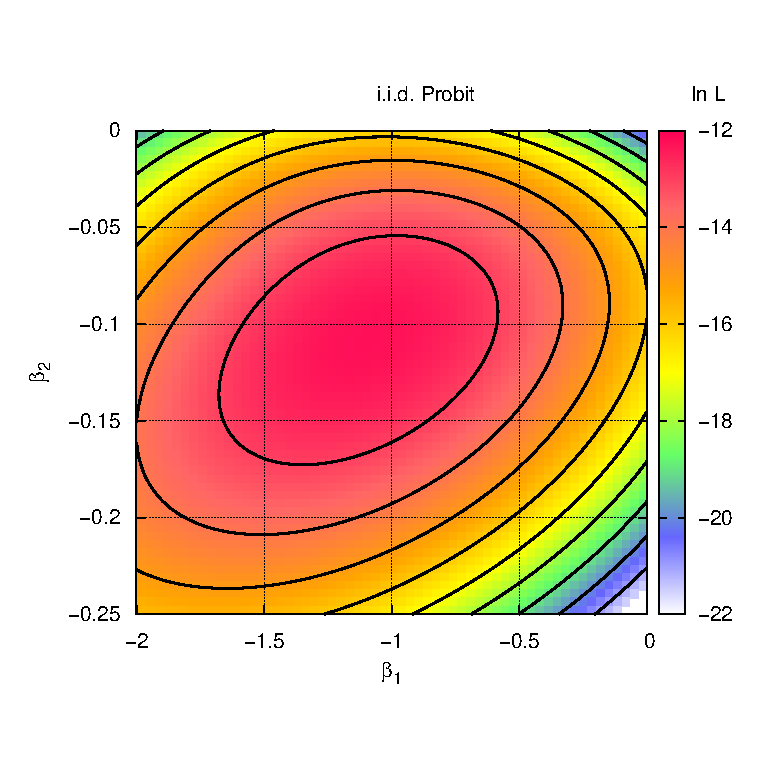
\includegraphics[width=0.5\textwidth]{./figsDiscr/kalProbitBinom_beta1beta2.eps}   
 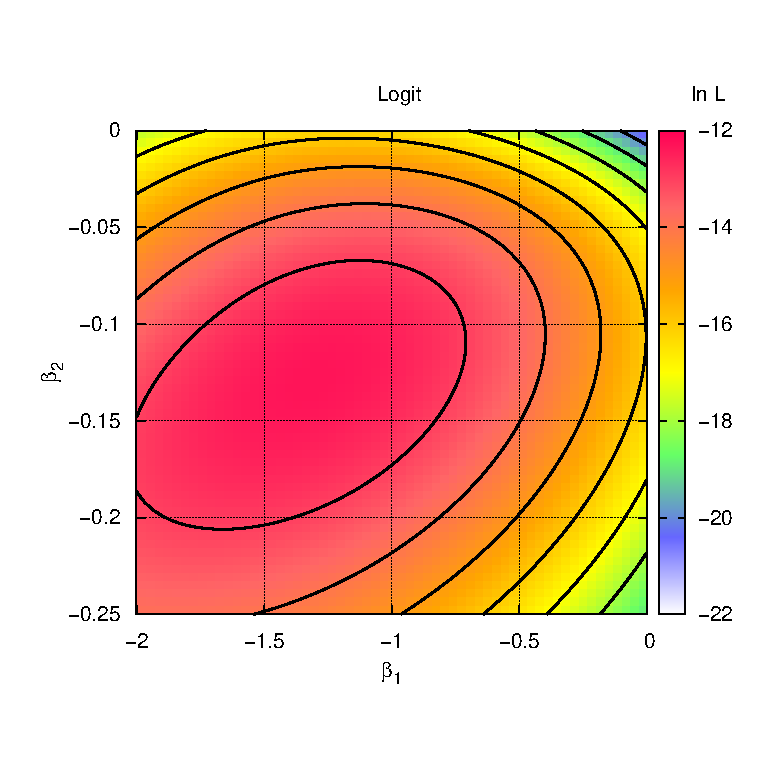
\includegraphics[width=0.5\textwidth]{./figsDiscr/kalLogitBinom_beta1beta2.eps}   
  \caption{\label{fig:logLbinom}Log-Likelihood (ohne den konstanten
Summanden $\sum_i \ln B_i$) des 
binomiale Probit-Modells (links) und des entsprechende Logit-Modells
(rechts) f\"ur die deterministische Nutzenfunktion
$V_{ni}=\beta_1\delta_{i1}+\beta_2 T_{ni}$
zu den in
Tabelle~\ref{tab:binomBeisp1} gegebenen Daten. Die deterministische
Nutzenfunktion ist jeweils in Einheiten von 
$\sigeps$ skaliert. Der Abstand einer ``H\"ohenlinie'' entspricht einer
Log-Likelihood-Differenz von 1.
}
\end{figure}
%###################################################
%
Abbildung~\ref{fig:logLbinom} zeigt, dass in beiden Modellen die
gesch\"atzten Werte $\hatbeta_1\approx -1.1$ und $\hatbeta_2 \approx -0.11$
in etwa gleich sind.\footnote{Siehe dazu entsprechende Beispiele im
  Lehrbuch von Meier/Weiss.}
 Dies ist konsistent mit Abb~\ref{fig:multiLogit},
da man aus ihr ablesen kann, dass bis etwa $I=4$ Alternativen und bei
Auswahlwahrscheinlichkeiten, welche nicht zu dicht an null oder eins
liegen, die 
Probit- und Logit-Auswahl\-wahr\-schein\-lich\-kei\-ten sich nur
geringf\"ugig 
unterscheiden.\footnote{Dann sind Abweichungen des Zufallsnutzens vom
Erwartungswert um mehrere Standardabweichungen relevant: Nur bei
derartigen Abweichungen unterscheiden sich die Normal- und die
Gumbelverteilungen deutlich.}
 Diese angen\"aherte Gleichheit der Parameterwerte
 gilt allerdings nur, wenn die Nutzenfunktionen gleich
skaliert sind, in der Regel  auf die Standardabweichung $\sigeps$ des
Zufallsnutzens. Andernfalls, insbesondere wenn man den Nenner
$\sqrt{2}$ im bin\"aren Probitmodell wegl\"asst oder die Parameter des
standardisierten Logit-Modells nicht nachtr\"aglich mit $\sqrt{6}/\pi$
multipliziert, erh\"alt man 
verschiedene Zahlenwerte der Parameter.
 Meist sind jedoch nur \emph{Quotienten}
der Parameter relevant, da diese (wegen der Skaleninvarianz)
Auswahlwahrscheinlichkeiten 
und abgeleitete Gr\"o\3en wie marginale Konsumneigungen, eine
Zahlungsbereitschaft (\emph{willingness to pay, WTP)} f\"ur gewisse Nutzen\"anderungen, 
Elastizit\"aten, subjektive Zeitwerte (\emph{value of travel time
  savings, VTTS)} und dergleichen
angeben. Bei Quotienten jedoch spielen unterschiedliche Skalierungen
keine Rolle, da sich diese weghebt, so dass wir folgendes wichtige
Ergebnis erhalten:

\maintext{F\"ur $I\le 4$ Alternativen und nicht zu extremen
  Auswahlwahrscheinlichkeiten, $P_{ni} \in [0.01, 0.99]$, sind die
  Quotienten gesch\"atzer Parameterwerte und damit marginale Kosten,
  Zeitwerte, Elastizit\"aten und andere gewonnene \"okonometrische
  Aussagen in Probitmodellen mit unkorrelierten Zufallsnutzen und in
  Logit-Modellen nahezu gleich.
}
%
 Im Beispiel bleibt der einzige Quotient $\hatbeta_1/\hatbeta_2$ 
unabh\"angig von der Skalierung und man erh\"alt in beiden Modellen nahezu denselben Wert:
\bdm
\left(\frac{\hatbeta_1}{\hatbeta_2}\right)\sub{Probit}=10, \quad
\left(\frac{\hatbeta_1}{\hatbeta_2}\right)\sub{Logit}=10.2
\edm
 Er gibt
an, dass die globale Bevorzugung f\"ur Alternative~2 (=globale
Benachteiligung von Alternative 1) etwa
\unit[10]{min} entspricht, Alterative~2 also im Mittel gleich h\"aufig
wie Alternative 1 gew\"ahlt wird, wenn sie eine um \unit[10]{min}
l\"angere komplexe Reisezeit aufweisen w\"urde.
Im Falle definiert skalierter Nutzenfunktionen (wie hier) gewinnt man
zus\"atzlich Information \"uber die Standardabweichung des
Zufallsnutzens, hier $-1/\beta_1 \approx \unit[9]{min}$.






%################################################################
\subsubsection{\label{sec:revealedChoiceEntf}Beispiel 2: 
Revealed-Choice Vorlesungsbefragung mit Entfernungen} 
%################################################################


Das folgenden Beispiele basiert auf eine unter Studenten
in den \"Okonometrie-Vorlesungen von 2007 bis 2011 durchgef\"uhrte
Umfragen, welches Verkehrsmittel 
(zu Fu\3, Rad, \"OV, MIV) am Befragungstag f\"ur
den Weg ``Wohnung-Uni'' gew\"ahlt wurde. Die Ergebnisse sind in 
Tabelle~\ref{tab:revealedChoiceMulti} dargestellt:
Zur einfacheren Datenerhebung in der Vorlesung  wurden die Daten aggregiert erfasst und
anstelle der individuellen 
Entfernungen nur Entfernungs\emph{klassen}
ber\"ucksichtigt. Der Index $n$ bedeutet damit keine einzelne Person,
soondern eine Klasse von Personen mit $y_n$ Mitgliedern. 
Es sei darauf hingewiesen, dass die Aggregierung  nur aufgrund der
schnelleren Datenerhebung sowie aus 
Gr\"unden der \"Ubersichtlichkeit gemacht wurde. Abgesehen davon 
verursacht sie nur unn\"otige Genauigkeitseinbu\3en, da dadurch
identische exogene Faktoren bei den Personen innerhalb jeder Gruppe
angenommen werden.
\begin{table}
\begin{center}
\begin{tabular}{|l||r|r|r|r||r|} \hline
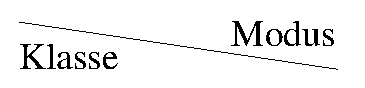
\includegraphics[width=9em]{figsGeneric/diagonal.eps} & $i=1$ (Fu\3) & $i=2$ (Rad)  
& $i=3$ (\"OPNV)  & $i=4$ (Kfz) & $y_n$\\
\hline\hline
$n=1$: 0-1 km  & 17 & 16 & 10 & 0 & 43 \\
$n=2$: 1-2 km  & 9 & 23 & 20 & 2 & 54 \\
$n=3$: 2-5 km  & 2 & 27 & 55 & 4 & 88 \\
$n=4$: 5-10 km & 0 & 7 & 42 & 7 & 56 \\
$n=5$: 10-20 km & 0 & 0 & 18 & 7 & 25 \\
 \hline
\end{tabular}
\end{center}
\caption{\label{tab:revealedChoiceMulti}Aggregierte Daten der 
Revealed-Choice-Befragungen in den \"Okonometrie-Vorlesungen 2007-2011.}
\end{table}



Um die Darstellung zu vereinfachen,  werden zun\"achst nur zwei Alternativen
unterschieden und folgende Aggregierungendurchgef\"uhrt:
\bi
\item Die ``langsamen'' nichtmotorisierten Verkehrsmittel Fu\3 und Rad werden zu
Alternative $i=1$ zusammengefasst,
\item die ``schnellen'' motorisierten Alternativen \"OPNV und MIV (motorisierter
Individualverkehr) zu Alternative 2.
\ei
Ferner wird f\"ur die Entfernung  -- mangels
detaillierter Informationen -- jeweils die Klassenmitte $r_n$ genommen.
Damit resultiert aus den urspr\"unglichen Daten  die Daten der
Tabelle~\ref{tab:revealedChoiceBin}.
%
\begin{table}
\begin{center}
\begin{tabular}{|l||r|r|r||r|} \hline
Klasse $n$ & \myBox{4em}{Klassen-\\mitte $r_n$} &
$i=1$ (Fu\3/Rad) & $i=2$ (\"OPNV/Kfz)  & $y_n$ \\
\hline\hline
$n=1$: 0-1 km  & \unit[0.5]{km} & 33 & 10 & 43 \\
$n=2$: 1-2 km  & \unit[1.5]{km} & 32 & 22 & 54 \\
$n=3$: 2-5 km  & \unit[3.5]{km} & 29 & 59 & 88\\
$n=4$: 5-10 km  & \unit[7.5]{km} & 7 & 49 & 56\\
$n=5$: 10-20 km  & \unit[15.0]{km} & 0 & 25 & 25 \\ \hline
\end{tabular}
\end{center}
\caption{\label{tab:revealedChoiceBin}Aggregierte Daten f\"ur die vereinfachte
  binomiale Formulierung der Revealed-Choice-Befragungen in
  den Vorlesungen.}
\end{table}
%
Die aggregierte deterministische Nutzenfunktion sei
gegeben durch
\be
\label{VdetRevealedChoiceBin}
V_{ni}(\beta_1,\beta_2) =\beta_1r_n\delta_{i1}+\beta_2\delta_{i1}.
\ee
Sie enth\"alt als Faktoren lediglich die alternativenspezifisch
formulierte Entfernung $x_{1ni}=r_n\delta_{i1}$ (Bewertung der
Entfernung bei Fu\3/Rad gegen\"uber der Referenz \"OV/MIV) 
und die alternativenspezifische Konstante $x_{2ni}=\delta_{i1}$ (globale
Pr\"aferenz Fu\3/Rad gegen\"uber der Referenz \"OV/MIV).

Da die
Entfernungen nicht nach Verkehrsmitteln unterschieden wurden, $r_{ni}=r_n$,
muss man die eigentlich generische Variable
``Entfernung'' formal wie eine soziodemographische Variable
behandeln: Bei ein und derselben Person sind ja in der Tat die
Entfernungen kaum unterschiedlich.
Insbesondere w\"are, im Gegensatz zum allgemeinen
Fall alternativenspezifisch formulierter generischer Variablen, 
das Modell durch einen weiteren Faktor $\beta_3r_n\delta_{i2}$ fehlspezifiziert.


%##########################################################
\begin{figure}
\fig{0.7\textwidth}{figsDiscr/BNL_Entfernung_2007-2011_logL.eps}
\caption{\label{fig:BNL-Entfernung-2007-2011-logL}Log-Likelihood des
  durch~\refkl{VdetRevealedChoiceBin} spezifizierten Binomial-Logit
  Modells bez\"uglich der Daten von
  Tabelle~\ref{tab:revealedChoiceBin}.
Die gesch\"atzten
Parameter sind $\beta_1=-0.46 \pm 0.05$ und
$\beta_2=1.1 \pm 0.2$
}
\end{figure}
%##########################################################


%##########################################################
\begin{figure}
\fig{0.7\textwidth}{figsDiscr/BNL_Entfernung_2007-2011_relHaeuf.eps}
\caption{\label{fig:BNL-Entfernung-2007-2011-relHaeuf}Nach
  Tabelle~\ref{tab:revealedChoiceBin} beobachtete und
  nach~\refkl{VdetRevealedChoiceBin} modellierte relative
  H\"aufigkeiten der Fu\3/Rad-Wege in den verschiedenen
  Entfernungsklassen f\"ur die Sch\"atzwerte $\hatbeta_1=-0.46$ und $\hatbeta_2=1.1$.
}
\end{figure}
%##########################################################

Da es nur zwei Parameter gibt, kann die Sch\"atzung direkt durch
Plotten der Log-Likelihood,
Abb.~\ref{fig:BNL-Entfernung-2007-2011-logL},
 vorgenommen werden.
Der aus der Abbildung entnehmbare Sch\"at\-zer $\hatbeta_1=-0.46$
bezieht sich auf die ``normale'' Logit-Skalierung in Vielfachem von
$pi/\sqrt{6}$ des Zufallsnutzens. Dies bedeutet, dass mit jedem zus\"atzlichen Kilometer die Attraktivit\"at der
Fu\3/Rad Wege um $0.46 \sqrt{6}/\pi \approx 0.35$
Zufallsnutzenunsch\"arfen gegen\"uber den
\"OV/MIV-Wegen abnimmt. Der Sch\"atzer $\hatbeta_2=1.1$ bedeutet, dass
bei der Entfernung $r=0$ die Option Fu\3/Rad gegen\"uber \"OV/MIV
einen Bonus von $1.1 \sqrt{6}/\pi \approx 0.9$
Zufallsnutzenunsch\"arfen hat: Man muss schon ein Amerikaner sein, um
bei einer Distanz von, z.B., \unit[100]{m} das Auto anzuwerfen.
Die aus der Abb.~\ref{fig:BNL-Entfernung-2007-2011-logL} entnehmbare
negative Korrelation zwischen $\hatbeta_1$ und $\hatbeta_2$ ist auch
anschaulich. Im Wesentlichen m\"ussen die Wahrscheinlichkeiten, also
die Nutzendifferenzen, f\"ur die am h\"aufigsten vorkommenden
mittleren Entfernungen richtig gesch\"atzt werden. Dort kann man einen
negativeren Entfernungsbeitrag f\"ur Fu\3/Rad-Wege ($\beta_1$
negativer) durch einen
positiveren globalen Bonus $\beta_2$ bei Entfernung null ($\beta_2$
positiver) teilweise kompensieren

Abbildung~\ref{fig:BNL-Entfernung-2007-2011-relHaeuf} stellt die
Aussagekraft des Modells durch einen Vergleich der beobach\-te\-ten
und gesch\"atzten relativen
H\"aufigkeiten dar (Quotient $y_{n1}/y_n$ bzw. Wahrscheinlichkeit
$P_{n1}=P_1(r_n)$). Man sieht, dass die
Aussageg\"ute ganz ordentlich ist. Die Nutzendifferenz
 $V_1-V_2=V_1$ ist null, falls $\beta_1
  r+\beta_2=0$, also bei einer Reiseweite
  $r=-\beta_2/\beta_1=\unit[2.4]{km}$. Bei dieser Entfernung sind also
  die modellierten Anteilswerte bzw. Entscheidungswahrscheinlichkeiten
  =0.5, was auch in der Abbildung zu sehen ist. 

Man beachte, dass die modellierten Wahrscheinlichkeitskurven
\emph{nicht} das Ergebnis einer LSE-Sch\"atzung sind. Letztere w\"urde
hier verzerrte Sch\"atzer liefern!




%#######################################
\subsection{\label{sec:maxLikelihoodDiscr}Kalibrierungsbedingungen
f\"ur das allgemeine Entscheidungsmodell}
%#######################################

Die \emph{grafische} Methode der Parametersch\"atzung unter direkter Verwendung der
Log-Likelihood~\refkl{logLAllg} des allgemeinen Entscheidungsmodells
st\"o\3t, unabh\"angig von der Zahl der Alternativen, bei mehr als zwei
Parametern an Grenzen: Die Log-Likelihoodfunktion $\tilL(\vec{\beta})$
kann man dann einfach nicht mehr
vollst\"andig plotten. Die \emph{funktionale} Sch\"atzung durch Maximierung von
$\tilL(\vec{\beta})$ bzw. Minimierung von  $-\tilL(\vec{\beta})$ ergibt als 
notwendige Bedingungen (Extremalwert) $M$ im Allgemeinen nichtlineare 
Gleichungen f\"ur die $M$
Parameter:
%\footnote{Bitte nicht den Parameterindex $j=1, \ldots, J$ oder die
%Indexgrenze $M$ mit der Log-Likelihood $\tilL(\vec{\beta})$
% oder der Likelihood $L(\vec{\beta})$ verwechseln!}

\maineq{kalibDiscrAllg}{
\ablpart{\tilL(\vec{\beta})}{\beta_m}=\sum\limits_{n=1}^N \sum\limits_{i=1}^I
 \frac{y_{ni}}{P_{ni}(\vec{\beta})} \ablpart{P_{ni}(\vec{\beta})}{\beta_m}=0.
}
Kompakt als Ableitung nach dem Parametervektor $\vecbeta$ geschrieben
(vgl. die Definitionen 
und Rechenregeln der Abschnitte~\ref{sec:matrixMult}
und~\ref{sec:matrixRules}), 
lauten die notwendigen Kalibrierungsbedingungen
\be
\label{kalibDiscrAllgVec}
\ablpart{\tilL(\vec{\beta})}{\vecbeta}=\sum\limits_{n=1}^N \sum\limits_{i=1}^I
 \frac{y_{ni}}{P_{ni}(\vec{\beta})} \ablpart{P_{ni}(\vec{\beta})}{\vecbeta}=\vec{0}.
\ee
%
Man kann f\"ur das Logitmodell und das i.i.d. Probitmodell zeigen,
dass bei parameterlinearen Nutzenfunktionen das 
so gefundene Extremum tats\"achlich ein globales Maximum
darstellt. Es gilt dann sogar weitergehend, dass die Likelihood- und
Loglikelihood-Funktionen global konkav,  also \"uberall ``nach unten
gekr\"ummt'' sind\footnote{McFadden, 
  \textit{Conditional logit analysis of qualitative choice behavior},
  Institute of Urban and Regional Development, University of
  California (1973).}  Damit sind~\refkl{kalibDiscrAllg} bzw.~\refkl{kalibDiscrAllgVec}
nicht nur notwendig sondern auch hinreichend.

 Die nichtlinearen Gleichungen~\refkl{kalibDiscrAllgVec} sind, abgesehen von
Trivialmodellen, nur numerisch l\"osbar. Dies geschieht mit
Methoden der \bfdef{nichtlinearen Optimierung}. Bekannte Verfahren
sind
\bi
\item das konzeptionell einfachste, aber bei Nichterf\"ullung der
  globalen Konvexit\"at
h\"aufig instabile \bfdef{Newton-Verfahren}
(vgl. Abschnitt~\ref{sec:discrAusw}),
\item das \emph{Gradient-Descent} Verfahren
(langsam, aber sicher),
\item \emph{Quasi-Newton-Verfahren}, welche ausnutzen, dass $\tilL(\vecbeta)$
  aus einer Summe von i.A. vielen Summanden besteht,
\item Verfahren wie der \emph{Broyden-Fletcher-Goldfarb-Shanno (BFGS)
  Algorithmus} oder der {Levenberg-Marquardt-Algorithmus}, welche die
  besten Eigenschaften des \emph{Gra\-di\-ent-Descent} und der
  \emph{Quasi-Newton-Verfahren} kombinieren. Speziell der
  BFGS-Algo\-rith\-mus wird in vielen \"okonometrischen Softwareprodukten 
  angewandt,
  \item \emph{Genetische Algorithmen}\footnote{Mit denen schie\3t man
    aber hier i.A. ``mit Kanonen auf Spatzen'', zumindest, wenn man a
    priori wei\3, dass es ein einziges globales Maximum gibt.}.
\ei
%
H\"aufig wird das BFGS-Verfahren angewandt.  Schwieriger wird es bei
parameter-nichtlinearen Nutzenfunktionen, welche beispielsweise bei der
Modellierung von \emph{Wahr\-neh\-mungs\-schwel\-len} ben\"otigt
(Abschnitt~\ref{sec:nonlinUtility}). Dann gilt folgende Warnung:

\maintext{Parameter-nichtlineare Nutzenfunktionen oder korrelierte
  Zufallsnutzen k\"onnen nicht nur
  zu nicht-konkaven Log-Likelihoods f\"uhren sondern auch zu welchen
  mit Nebenmaxima (vgl. Abb.~\ref{fig:nonlinUtility1}). 
Dann l\"auft jede der obigen Methoden  Gefahr, sich in
  ein solches zu ``verrennen''. Das Risiko wird durch einen m\"oglichst guten
  \emph{initial guess} sowie ggf durch die Wahl von
  \emph{genetische Algotrithmen} minimiert.}

Eine wichtige Rolle wird sp\"ater auch die symmetrische $M\times M$
\bfdef{Hesse-Matrix} der zweiten 
Ableitungen von $-\tilL$ spielen.\footnote{Damit kann man die Eigenschaft, dass die
  Log-Likelihoodfunktion global konkav bzw. $-\tilL$ global konvex
  ist, genauer definieren: die Hesse-Matrix der zweiten Ableitungen
  von $-\tilL$ ist \"uberall
positiv definit.}  Die negative Hesse-Matrix an der Stelle $\vecbeta=\hatvecbeta$
wird, auch aus sp\"ater klar werdenden Gr\"unden,
\bfdef{Informationsmatrix} genannt:
\be
\label{HesseL}
H_{jm}=-\ablpartmix{\tilL(\hatvecbeta)}{\beta_j}{\beta_m}
\quad \text{bzw.} \quad
\m{H}=-\ablpartmix{\tilL(\hatvecbeta)}{\vecbeta}{\vecbeta\tr}.
%=\sum\limits_n \sum\limits_i \left(
%-\frac{y_{ni}}{P^2_{ni}}\ablpart{P_{ni}}{\beta_j}\ablpart{P_{ni}}{\beta_m}
%+\frac{y_{ni}}{P_{ni}}\ablpartmix{P_{ni}}{\beta_j}{\beta_m}
%\right)
\ee
%
Im folgenden wird die Maximum-Likelihood-Methode f\"ur
die bisher vorgestellten Modelle spezialisiert.


%#######################################
\subsection{\label{sec:maxLikelihoodBinom}Sch\"atzung des
binomialen Probit-Modells mit quasilinearen Nutzen}
%#######################################

Skaliert man die Nutzenfunktionen in Einheiten 
der Standardabweichung $\sigeps$ des Zufallsnutzens, ergeben sich 
nach~\refkl{binProbit} die Auswahlwahrscheinlichkeiten des 
Probitmodells zu
\bdm
P_{n1}(\vecbeta)=\Phi
\left(\frac{V_{n1}(\vecbeta)-V_{n2}(\vecbeta)}{\sqrt{2}}\right),
\quad  
P_{n2}(\vecbeta)=1-P_{n1}(\vecbeta).
\edm
Die Ableitung der Wahlwahrscheinlichkeiten
$P_{ni}(\vecbeta)$ ergeben f\"ur
parameterlineare Nutzenfunktionen
der Art~\refkl{Vquasilin}, also $V_{ni}=\vecbeta\tr\vec{x}_{ni}$, die Bedingungen
\bdma
\ablpart{P_{n1}}{\vecbeta}
 &=& \frac{1}{\sqrt{2}} f_N\left(\frac{V_{n1}-V_{n1}}{\sqrt{2}}\right)
 \ablpart{}{\vecbeta}\left(V_{n1}-V_{n1}\right) \\
 &=& \frac{1}{\sqrt{2}} f_N\left(\frac{V_{n1}-V_{n1}}{\sqrt{2}}\right)
  \left(\vec{x}_{n1}-\vec{x}_{n2}\right), \\
\ablpart{P_{n2}}{\vecbeta} &=& - \ablpart{P_{n1}}{\vecbeta}.
\edma
Hierbei ist $f_N(x)=\Phi'(x)=1/\sqrt{2\pi} e^{-x^2/2}$ 
die Dichtefunktion der Standardnormalverteilung. 
Setzt man dies in~\refkl{kalibDiscrAllgVec} ein, erh\"alt man

\maineq{kalibBProbit}{
\ablpart{\tilL(\vec{\beta})}{\vecbeta}
 = \frac{1}{\sqrt{2}}
\sum\limits_{n=1}^N \left(\frac{y_{n1}}{P_{n1}}-\frac{y_{n2}}{P_{n2}}\right)
   f_N\left(\frac{V_{n1}-V_{n2}}{\sqrt{2}}\right)
 \left(\vec{x}_{n1}-\vec{x}_{n2}\right)=0.
\qquad \text{\parbox{7em}{Kalibrierung\\binomiales\\Probitmodell.}}
}
%
%Die Informationsmatrix ist gegeben durch (vgl. wieder die Definitionen
%und Rechenregeln der Abschnitte~\ref{sec:matrixMult} und~\ref{sec:matrixRules})
%\be
%\label{mH-BProbit}
%\m{H}=-\ablpartmix{\tilL}{\vecbeta}{\vecbeta\tr}
%= \frac{1}{2} \sum\limits_{n=1}^N \left[
%\left(\frac{y_{n1}}{P^2_{n1}}+\frac{y_{n2}}{P^2_{n2}}\right) f_N^2\left(\frac{V_{n1}}{\sqrt{2}}\right)
% + \left(\frac{y_{n2}}{P_{n2}}-\frac{y_{n1}}{P_{n1}}\right) f'_N\left(\frac{V_{n1}}{\sqrt{2}}\right)
%\right] \vec{x}_{n1}\, \vec{x}_{n1}\tr.
%\ee


%#######################################
\subsection{\label{sec:maxLikelihoodMNL}Sch\"atzen der Logit-Modelle mit quasilinearen Nutzen}
%#######################################

F\"ur die MNL-Auswahlwahrscheinlichkeiten \refkl{MNL}, also
$P_{ni}=e^{V_{ni}}/\sum_{i'}e^{V_{ni'}}$  erh\"alt man f\"ur die
Log-Likelihood $\tilL=\sum_{n,i}y_{ni} \ln P_{ni}$ direkt
\be
\label{lMNLAllg}
\tilL(\vec{\beta})=\sum\limits_{n, i} \left[y_{ni}\left(V_{ni}
-\ln \sum\limits_{i'}e^{V_{ni'}}\right)\right]
\ee
und durch Ableiten und Nullsetzten (nichttrivial, Interessierte sehen die Herleitung
in Abschnitt \ref{sec:discrHerl} nach!) die Kalibrierungsgleichungen
\be
\label{kalibMNLAllg}
\ablpart{\tilL(\vec{\beta})}{\vecbeta}
=\sum\limits_{n, i} 
\bigg[ y_{ni}- P_{ni}(\vec{\beta})\bigg]
\ablpart{V_{ni}(\vec{\beta})}{\vecbeta} = \vec{0}.
\ee
Hierbei wurde die Doppelsumme verk\"urzt geschrieben:
$\sum_{n=1}^N\sum_{i=1}^I=\sum_{n,i}$. 
Dies sind $M$ nichtlineare Gleichungen f\"ur die $M$ Parameter $\beta_m$.
In Worten lautet die $m$-te Bedingung:

\maintext{Die Summe (\"uber alle Alternativen und Personen bzw. Choice
  Sets) der mit
dem Grenznutzen bez\"uglich $\beta_m$ gewichteten
Differenzen zwischen den gemessenen und vom Modell
erwarteten absoluten H\"aufigkeiten muss f\"ur alle $m=1, ..., M$ verschwinden.
}
\vspace{1em}

\noindent 
Der praktisch wichtigste Fall sind quasilineare deterministische
Nutzenfunktionen gem\"a\3 Gl. \refkl{Vquasilin}, also 
$V_{ni}=\vecbeta\tr\vec{x}_{ni}$. Dann wird
\refkl{kalibMNLAllg} zum (allerdings immer noch nichtlinearen)
Gleichungssystem  

\maineq{kalibMNL}{
\ablpart{\tilL(\hatvecbeta)}{\vecbeta}
=\sum\limits_{n, i}  \big[ y_{ni} - P_{ni}(\hatvecbeta)\big] \, \vec{x}_{ni}
=\vec{0}. \qquad \text{\parbox{6em}{Kalibrierung\\MNL-Modell.} }
}
Dies kann man anschaulicher ausdr\"ucken, wenn man
\bfdef{Merkmalssummen} als Summe der exogenen Faktoren $x_{nmi}$
\"uber alle Alternativen und Personen definiert:
\be
\label{Merkmalssumme}
X_m=\sum_{n, i} y_{ni} x_{nmi}, \quad \text{bzw.} \quad 
\vec{X}=\sum_{n, i} y_{ni} \vec{x}_{ni}
\ee
Dann lauten die MNL-Kalibrierungsbedingungen f\"ur quasilineare
deterministische Nutzen $V_{ni}=\vecbeta\tr\vec{x}_{ni}$ schlicht und
ergreifend
\maintext{Der vom MNL gesch\"atzte Vektor $\vec{X}\sup{MNL}$ 
der Merkmalssummen muss gleich dem beobachteten Merkmalssummen-Vektor 
$\vec{X}\sup{data}$ sein, also muss f\"ur alle Komponenten $m$ gelten
\bdm
X_m\sup{MNL}=X_m\sup{data}, \quad \quad 
X_m\sup{MNL}=\sum_{n, i} P_{ni}(\hatvecbeta)\, x_{nmi},\quad
X_m\sup{data}=\sum_{n, i} y_{ni}\, x_{nmi} = \sum_n x_{nmi_n}.
\edm
\vspace{-1em}
}


\subsubsection*{Prinzip-Beispiel f\"ur vier Einflussfaktoren}
Der quasilineare deterministische Nutzen zweier Verkehrsmodi $i$ sei
gem\"a\3 folgender Gleichung 
 aus vier  Kriterien bzw. Einflussfaktoren 
zusammengesetzt:
\bdm
V_{ni}=\vecbeta\tr\vec{x}_{ni}=\sum_{m=1}^4\beta_mx_{nmi}
 =\beta_1T_{ni}+\beta_2K_{ni}+\beta_3 g_i \delta_{i1}+\beta_4\delta_{i1}.
\edm
mit
\bi
\item $x_{1ni}=T_{ni}$ der komplexen Reisezeit f\"ur Person $n$ bei Wahl des
  Verkehrsmodus $i$,
\item $x_{2ni}=K_{ni}$ die zugeh\"origen (Grenz-)Kosten,
\item $x_{3ni}=g_n\delta_{i1}$ der exogene Faktor  f\"ur das Geschlecht mit
$g_{\male}=0$ und $g_{\female}=1$,
\item $x_{4ni}=\delta_{i1}$ der alternativen spezifischen Konstante
  (Referenz ist Alternative~2).
\ei
%
Die MNL-Sch\"atz- bzw. Kalibrierungsbedingungen der vier zugeh\"origen Parameter lauten

\paragraph{Faktor 1: Komplexe Reisezeit.} Die \emph{Merkmalssumme} $X_1$ ist 
gleich der Gesamtreisezeit $T$ bei
Umsetzung aller Entscheidungen. Die zugeh\"orige \emph{Sch\"atzbedingung} lautet
\bdm
T\sup{data}=T\sup{MNL}(\vecbeta)
\edm
mit
\bdm
\begin{array}{lll}
T\sup{data}&=\sum_{n,i} y_{ni} T_{ni} & \text{Realisierte Gesamtreisezeit,}  \\
T\sup{MNL}(\vecbeta)&=\sum_{n,i} P_{ni}(\vecbeta)T_{ni}
 & \text{modellierte Gesamtreisezeit.}  \\
\end{array}
\edm

\paragraph{Faktor 2: (Grenz-)Kosten.} Die \emph{Merkmalssumme} $X_2$ ist
gleich den Gesamtkosten $K$ bei
Umsetzung aller Entscheidungen. Die zugeh\"orige \emph{Sch\"atzbedingung}
lautet in Analogie zu den Reisezeiten
\bdm
K\sup{data}=K\sup{MNL}(\vecbeta)
\edm
mit
\bdm
\begin{array}{lll}
K\sup{data}&=\sum_{n,i} y_{ni} K_{ni} & \text{Realisierte Gesamtkosten,}  \\
K\sup{MNL}(\vecbeta)&=\sum_{n,i}  P_{ni}(\vecbeta)K_{ni}
 & \text{modellierte Gesamtkosten.} \\
\end{array}
\edm

\paragraph{Faktor 3: Bevorzugung der Alternative 1 bei Frauen.}
  Dieser Faktor ist, wie bei sozio\"okonomischer Variable gefordert, 
 alternativenspezifisch
formuliert.
Die \emph{Merkmalssumme} 
$X_3=\sum_{n,i}y_{ni}g_n\delta_{i1}=\sum_{n} y_{n1}g_n=N_{1,\female}$
 ist die Anzahl der von Frauen
getroffenen Entscheidungen zugunsten Alternative 1. Die zugeh\"orige
\emph{Sch\"atzbedingung} 
lautet
\bdm
N_{1,\female}\sup{data}=N_{1,\female}\sup{MNL}(\vecbeta)
\edm
mit
\bdm
\begin{array}{lll}
N_{1,\female}\sup{data} &=\sum_{n} y_{n1} g_n & \text{Realisierte
  Entscheidungszahl f\"ur Alt.~1 bei Frauen,} \\
N_{1,\female}\sup{MNL}(\vecbeta) &=\sum_{n}  P_{n1}(\vecbeta)g_n
 & \text{modellierte Entscheidungszahl f\"ur Alt.~1 bei Frauen.}  \\
\end{array}
\edm 

\paragraph{Faktor 4: Globale Bevorzugung der Alternative 1.} Die
  Sch\"atzung der alternativenspezifischen Konstante geht analog wie die der
  alternativenspezifischen sozio\"okonomischen Variable.
Die \emph{Merkmalssumme} $X_4=\sum_{n,i}y_{ni}\delta_{i1}=\sum_{n} y_{n1}=N_1$ ist die Gesamtzahl der zugunsten Alternative 1
getroffenen Entscheidungen. Die zugeh\"orige \emph{Sch\"atzbedingung}
lautet
\bdm
N_1\sup{data}=N_1\sup{MNL}(\vecbeta)
\edm
mit
\bdm
\begin{array}{lll}
N_1\sup{data} &= \sum_n y_{n1} 
  & \text{Realisierte
  Gesamt-Entscheidungszahl f\"ur Alt.~1}  \\
N_1\sup{MNL}(\vecbeta) &=\sum_{n} P_{n1}(\vecbeta)
  & \text{modellierte Gesamt-Entscheidungszahl f\"ur Alt.~1.} \\
\end{array}
\edm



%#########################################################
\subsection{\label{sec:konstantenmodell}Sch\"atzung des Konstantenmodells}
%##########################################################
%
Das Konstantenmodell hat keine personenabh\"angigen exogenen
Variablen, nur einen vollst\"andigen Satz an alternativenspezifischen
Konstanten (ACs). Mit der Referenzalternative $i=I$ lauten seine
deterministischen Nutzenfunktionen
\be
\label{konstantenmodell} 
V_{ni}=\sum_{j=1}^{I-1}\beta_j\delta_{ji},
\ee
Neben dem Nullmodell (alle Nutzenfunktionen sind =0) ist das
Konstantenmodell ein wichtiges Referenzmodell zur Definition globaler
G\"utema\3e wie dem \emph{Likelihood-Ratio-Index}
(vgl. Abschnitt~\ref{sec:gueteDiscr} weiter unten).

\subsubsection*{Sch\"atzung auf der Ebene der vorausgesagten Wahrscheinlichkeiten}
%
F\"ur beliebige Alternativenzahl und beliebige Spezifikationen des Zufallsnutzens  
(Logit, Probit und andere, mit oder ohne Korrelationen) kann die
Sch\"atzung auf der Ebene der vorausgesagten Wahrscheinlichkeiten
$P_{ni}$ allgemein durchgef\"uhrt werden. Hierzu ben\"otigen wir nur
die Tatsache, dass aufgrund des Fehlens personenspezifischer Merkmale
die modellierte Wahrscheinlichkeit $P_{ni}=P_i$ nicht von der Person
$n$ abh\"angt. Damit ist die Log-Likelihood-Funktion
\bdma
\tilL(\vec{P}) &=& \sum_{ni}y_{ni}\ln P_{ni} \\
 &=& \sum_{ni}y_{ni}\ln P_i \\
 &=& \sum_i \left(\sum_n y_{ni}\right) \ln P_i \\
 &=& \sum_i N_i \ln P_i.
\edma
mit $N_i=\sum_n y_{ni}$ der Zahl der realisierten Entscheidungen f\"ur
Alternative $i$. 

Um dies jetzt nun bez\"uglich der Wahrscheinlichkeiten zu maximieren,
muss man die Nebenbedingung $\sum_i P_i=1$
ber\"ucksichtigen.\footnote{Andernfalls ist das Ergebnis
  unbeschr\"ankt und alle $P_i\to\infty$ w\"aren das ``Optimum''} 
\footnote{Streng genommen m\"usste man auch $P_i \ge 0$ und $P_i \le
  1$ fordern. Das Ergebnis erf\"ullt jedoch auch ohne diese
  Restriktionen diese Nebenbedingungen, so dass diese nicht
  \emph{relevant} sind.} Dies wird durch die Technik der sogenannten
\emph{Lagrange-Multiplikatoren} realisiert: 

\maintext{Maximierung/Minimierung
%\hspace{0.05\textwidth}\parbox{0.9\textwidth}{Maximierung/Minimierung
  einer Funktion $f(\vec{x})$ mit Nebenbedingung $g(\vec{x})=0$: Leite
  nicht nur die Funktion ab und setze sie 
  null, sondern die Funktion abz\"uglich der mit dem
  \emph{Lagrange-Multiplikator} $\lambda$ multiplizierten
  Nebenbedingung. Die Nebenbedingung muss dabei in der obigen Form $g(\vec{x})=0$
  vorliegen. Bei mehreren Nebenbedingungen gibt es analog mehrere Lagrangeparameter}

Hier ergibt dies
\bdm
\ablpart{}{P_i} \left(\sum_i N_i \ln P_i - \lambda \sum_i P_i\right)
= \frac{N_i}{P_i}-\lambda \stackrel{!}{=} 0,
\edm
also $P_i=N_i/\lambda$. Der noch unbekannte Lagrange-Parameter wird
durch Einsetzen in die Nebenbedingung bestimmt:
\bdm
\sum_i P_i=\sum_i \frac{N_i}{\lambda}=\frac{N}{\lambda}=1
\ \Rightarrow \ \lambda=N
\edm
und damit
\be 
\label{kalib-konst-P}
P_i\sup{Konstantenmodell}=\frac{N_i}{N}=f_i
\ee
In Worten: Die prognostizierten Wahrscheinlichkeiten des kalibrierten
Konstantenmodells sind 
gleich den realisierten relativen H\"aufigkeiten.

\subsubsection*{Direktsch\"atzung der Parameter des Multinomial-Logit-Modells}
Setzt man die MNL-Formel~\refkl{MNL} mit den deterministischen
Nutzenfunktionen~\refkl{konstantenmodell} in~\refkl{kalib-konst-P} ein, erh\"alt
man f\"ur die Quotienten (nicht alle F\"alle sind aufgef\"uhrt)
\bdm
\frac{P_i}{P_j}=\frac{f_i}{f_j}=e^{V_i-V_j}
=\twoCases{e^{\beta_i-\beta_j}}{i \neq I, j\neq I}{e^{\beta_i}}{i \neq I, j=I}
\edm
Aus dem letzteren Fall direkt
\be
\label{kalib-konst-MNL}
\beta_i\sup{MNL,Konstantenmodell}=\ln\left(\frac{f_i}{f_I}\right)
 =\ln\left(\frac{N_i}{N_I}\right).
\ee

\subsubsection*{Direktsch\"atzung der Parameter des binomialen
  Probit-Modells}

F\"ur das binomialen
  Probit (BP) Modell gilt (mit der Referenzalternative $I=2$, also
  $V_1=\beta_1, V_2=0$): 
\bdm
P_1=\Phi\left(\frac{V_1-V_2}{\sqrt{2}}\right)
=\Phi\left(\frac{\beta_1}{\sqrt{2}}\right)
\edm
also
\be
\label{kalib-konst-BP}
\beta_i\sup{BP,Konstantenmodell}=\sqrt{2}\Phi^{-1}\left(\frac{N_1}{N}\right),
\ee
wobei $\Phi^{-1}(.)$ die Umkehrfunktion (Quantilsfunktion) der
Standardnormalverteilung bezeichnet.


%#########################################################
\section{\label{sec:discrAusw}Numerische L\"osung der
Sch\"atzgleichungen mit der Newton-Methode}
%##########################################################
Das Vorgehen wird f\"ur den praktisch wichtigsten Fall der
Logit-Modelle mit parameterlinearen Nutzen 
gezeigt, ist aber analog auch auf die Probitmodelle
anwendbar. Es wird das konzeptionell einfache 
\bfdef{Newton'sche Iterationsverfahren} vorgestellt, welches meist in
 wenigen Schritten konvergiert, im Allgemeinen aber auch instabil
 sein kann (Abschnitt~\ref{sec:maxLikelihoodDiscr}). 
F\"ur Logitmodelle mit parameterlinearen Nutzen ist
 $\tilL$ jedoch global konkav, was gleichbedeutend damit ist, das das
 Newton'sche Verfahren \emph{immer} konvergiert.


Die Bedingung \refkl{kalibMNL} wird zun\"achst als  Standardform
einer nichtlinearen multivariaten Nullstellensuche geschrieben: Der
Gradient $\vec{g}$ der negativen Log-Likelihood\footnote{Der positive
  Gradient $\partial \tilL/\partial\vecbeta$ wird in der englischsprachigen Literatur oft als
  \emph{score} bezeichnet. Mit der \"ublichen Bedeutung
  (``Ergebnis'') hat das aber nichts zu tun.}
 muss gleich null sein:
\maineq{Gzero}{
\vec{g}(\vec{\beta})=-\ablpart{\tilL}{\vecbeta}
=\sum\limits_{n,i} \left[P_{ni}(\vec{\beta})-y_{ni}\right]
    \vec{x}_{ni} \stackrel{!}{=} \vec{0}.
}
Der Gradient der Logit-Modelle 
enth\"alt als Komponenten also genau die Merkmalssummen-Differenzen!
F\"ur die Probitmodelle ergeben sich der Gradient $\vec{g}$
aus~\refkl{kalibDiscrAllgVec}. 
Hinreichend nahe der gesuchten Nullstelle $\hatvecbeta$ mit
$\vec{g}(\hatvecbeta)=0$ gilt
\be
\label{TaylorMulti}
\vec{g}(\vec{\beta}) \approx g(\hatvecbeta)
+ \m{H}\cdot (\vec{\beta}-\hatvecbeta)
= \m{H}\cdot (\vec{\beta}-\hatvecbeta).
\ee
wobei die Hesse- bzw. Informationsmatrix
$\m{H}=\ablpart{\vec{g}}{\vecbeta}=-\ablpartmix{\tilL}{\vecbeta}{\vecbeta\tr}$
durch~\refkl{HesseL} gegeben ist. F\"ur die Logitmodelle
ergeben sich (vgl. wieder 
Abschnitt \ref{sec:discrHerl} f\"ur eine Herleitung)
\bi
\item im allgemeinen multinomialen Fall ($I\ge 2$ Alternativen)
\maineq{mH-MNL}{
\m{H}=\sum\limits_{n,i}P_{ni}\,\vec{x}_{ni}
\left(\vec{x}_{ni}\tr- \sum\limits_{i'}\vec{x}_{i'i}\tr\,P_{i'i}\right),
}
\item im binomialen Fall ($I=2$ Alternativen) bei Verlagerung des
 gesamten deterministischen Nutzens auf
Alternative 1
\be
\label{mH-BNL}
\m{H}=\sum\limits_n P_{n1}\, P_{n2}\, \vec{x}_{n1}\, \vec{x}_{n1}\tr.
\ee
\ei
Um einen Iterationsschritt zu formulieren, l\"ost man
die Gleichung~\refkl{TaylorMulti} nach dem gesuchten
Sch\"atzwert $\hatvecbeta$ des Koeffizientenvektors auf, wozu eine
Multiplikation mit $\m{H}^{-1}$
notwendig ist:
\be
\label{TaylorMultii}
\hatvecbeta \approx \vec{\beta} - \m{H}^{-1} \vec{g}(\vec{\beta}).
\ee
Da \refkl{TaylorMulti} nur eine N\"aherung ist, gilt dies auch 
f\"ur die gerade hergeleitete
Beziehung. Ist man jedoch nicht zu weit von $\hatvecbeta$
entfernt oder ist $\tilL$ global konkav, konvergiert fortlaufendes
Einsetzen der rechten Seite in die 
linke meist sehr rasch. H\"aufig kann man als Startbedingung
$\vec{\beta}=\vec{0}$ ansetzen. Die numerische Berechnung der
Kalibrierungsbedingungen des MNL mit
quasilinarer Nutzenfunktion ist also durch folgendes ``Rezept''
gegeben:
\maineq{kalibMNLnum}{
\begin{array}{rcl}
\text{Startbedingung} &:&  \vec{\beta}^{(0)}=\vec{0},\\
\text{$i$-te Iteration} &:& \vec{\beta}^{(i+1)}=\vec{\beta}^{(i)}
- \left(\m{H}(\vec{\beta}^{(i)}) \right)^{-1}
  \vec{g} \left(\vec{\beta}^{(i)} \right),\\
\text{Ergebnis nach $I$-ter Iteration} &:&
\hatvecbeta \approx \vec{\beta}^{(I+1)}
\end{array}
}
%
Die Abbruchbedingung f\"ur die letzte Iteration $I$ kann man
beispielsweise daran festmachen, dass sich in diesem Iterationsschritt
alle Sch\"atzer relativ um nicht mehr als $\delta$ (z.B. $\delta=10^{-3}$) \"andern:
\be
\label{MNLkalib-abbruch}
\frac{\beta_m^{(I+1)}-\beta_m^{(I)}}{\beta_m^{(I+1)}} < \delta \quad \forall
m=1, ..., M.
\ee
%

\verstaendnisbox{Wie schnell konvergiert das Newton-Verfahren, wenn die
in $\vec{g}$ zusammengefassten Funktionen 
$g_m=-\ablpart{\tilL}{\beta_m}$ linear in den Parametern $\vec{\beta}$
sind? {\scriptsize Antwort: Eine Iteration liefert das exakte Ergebnis}
}


%################################################################
\subsection{Beispiel: Revealed-Choice-Befragung mit zwei Alternativen}
%################################################################
%
Es wird wieder die im zweiten Beispiel des
Abschnitts~\ref{sec:kalibrGrafisch} beschriebene Vorlesungsbefragung
der Verkehrsmittelwahl in Abh\"angigkeit der Entfernungen betrachtet.
Ferner wird wie dort die Situation  gem\"a\3
Tabelle~\ref{tab:revealedChoiceBin} auf zwei Alternativen reduziert. Das 
Binomial-Logit-Modell mit den Nutzenfunktionen~\refkl{VdetRevealedChoiceBin},
\bdm
V_{ni}(\beta_1,\beta_2) =\beta_1r_n\delta_{i1}+\beta_2\delta_{i1},
\edm
ist dasselbe wie bei der grafischen L\"osung, das Modell wird aber nun 
mumerisch mit dem Newton-Verfahren gesch\"atzt. 

Wir nehmen als Anfangsbedingung 
$\vecbeta\tr=(0,0)$ an. Es ist zu vermuten, dass dies
nicht die kalibrierten Werte sind, so dass sich die realisierten und
vom Modell gesch\"atzten Merkmalssummen wohl unterscheiden. Dies wird
nun untersucht:

\paragraph{Faktor 1: Entfernung zu Fu\3 oder mit dem Rad.} Die Merkmalssumme $X_1$ ist 
gleich der Gesamtentfernung
$R_1$ zu Fu\3 oder mit dem Rad. Die zugeh\"orige \emph{Sch\"atzbedingung} lautet
\bdm
R_1\sup{data}=R_1\sup{MNL}(\vecbeta).
\edm
Die Realisierung mit den Daten und die Sch\"atzung durch das Modell
mit $\vecbeta\tr=(0,0)$, also $P_{n1}=P_{n2}=0.5$, ergibt 
\bdm
\begin{array}{lll}
R_1\sup{data}
 &= \sum_n y_{n1}r_n=\uu{\unit[218.5]{km}} 
 &  \text{realisierte Gesamtentfernung Fu\3/Rad,}  \\ 
R_1\sup{MNL}(0,0)
 &= \frac{1}{2} \sum_n y_n r_n=\uu{\unit[608.25]{km}} 
 &  \text{modellierte Gesamtentfernung Fu\3/Rad.}  \\
\end{array}
\edm
Man beachte, dass hier jeweils $y_n=\sum_i y_{ni}$  gleichartige
Entscheidungssituationen (f\"ur die verschiedenen Entfernungsklassen)
zusammengefasst wurden, was den zus\"atzlichen Faktor $y_n$ bei der
modellierten Merkmalssumme begr\"undet. 

\paragraph{Faktor 2: Alternativenspezifische Konstante (AC) der Alternative 1.} 
Die Merkmalssumme $X_2$ ist die Gesamtzahl der
Wahlentscheidungen f\"ur Alternative~1: 
Die zugeh\"orige \emph{Sch\"atzbedingung}
lautet
\bdm
N_1\sup{data}=N_1\sup{MNL}(\vecbeta)
\edm
mit
\bdm
\begin{array}{lll}
N_1\sup{data} 
  &= \sum_n y_{n1} =\uu{101}
  & \text{realisierte Entscheidungszahl Fu\3/Rad,}  \\
N_1\sup{MNL}(0,0) 
  &= \frac{1}{2} \sum_n y_n =\uu{144}
  & \text{modellierte Entscheidungszahl Fu\3/Rad.}  \\
\end{array}
\edm
%
Die realisierten und modellierten
Merkmalssummen differieren stark, so dass offensichtlich
 $\vecbeta\tr=(0,0)$ nicht der richtige Sch\"atzvektor ist.
Insbesondere wird zu Fu\3 und mit
dem Rad eine viel zu hohe Entfernung zur\"uckgelegt, da bei
$\vecbeta=\vec{0}$ die Auswahlwahrscheinlichkeiten immer $P_{ni}=1/2$
betragen, auch bei den langen Wegen. 

Um das Newton-Verfahren anzuwenden,  ben\"otigen wir noch das Inverse der Hessematrix:

\bdm
\m{H}=\myMatrixTwo{H_{11} & H_{12}\\ H_{21} & H_{22}}
\quad \Rightarrow \quad 
 \m{H}^{-1}=\frac{1}{\text{Det} (\m{H}) }
\myMatrixTwo{H_{22} & -H_{12}\\ -H_{21} & H_{11}}.
\edm
\vspace{0.5em}

\noindent
Damit kann man die Newton-Iterationsgleichungen~\refkl{kalibMNLnum}
schreiben als

\bea
\label{NewtonTwo}
\myVector{\beta_1 \\ \beta_2}^{(i+1)}
&=& \myVector{\beta_1\\ \beta_2}^{(i)} 
- \frac{1}{\text{Det} (\m{H}^{(i)}) }
\begin{pmatrix} H_{22} &-H_{12}\\-H_{21}& H_{11}\end{pmatrix}^{(i)}
\cdot \myVector{g_1\\g_2}^{(i)} \nonumber \\
&=& \left[\myVector{\beta_1\\ \beta_2} 
- \frac{1}{\text{Det} (\m{H}) }
\myVector{H_{22}g_1-H_{12} g_2 \\ -H_{21} g_1+H_{11} g_2}
\right]^{(i)}.
\eea
%
Die Matrixelemente werden mit \refkl{mH-BNL} berechnet:

\bdma
H_{11} &=& \sum\limits_n r_n^2 P_{n1}P_{n2}, \\
H_{12}=H_{21} &=& \sum\limits_n r_n P_{n1}P_{n2}, \\
H_{22} &=& \sum\limits_n P_{n1}P_{n2}.
\edma
Startet man die Newton-Iteration mit $\vecbeta=\vec{0}$, ergibt sich
folgender Verlauf, wobei als Kontrolle auch die beiden
Merkmalssummendifferenzen (Komponenten des Gradients $\vec{g}$)
aufgef\"uhrt sind:
\bdm
\begin{array}{|c||l|l||l|l|}  \hline
\text{Iteration} & \beta_1 & \beta_2 
& \myBox{10em}{$g_1=X_1\sup{MNL}-X_1\sup{data}$}
& \myBox{10em}{$g_2=X_2\sup{MNL}-X_2\sup{data}$} \\ \hline
0 &  0.000000 & 0.00000 & 384.25 & 32 \\
1 & -0.211613 & 0.47782 & 99.70 & 7.33\\ 
2 & -0.356599 & 0.85944 & 30.21 & 2.570\\
3 & -0.439557 & 1.05873 & 4.70891 & 0.48637 \\
4 & -0.456050 & 1.09507  & 0.144063 & 0.0163218 \\
5 & -0.456565 & 1.09616 & 1.37*10^{-4} & 1.60 * 10^{-5}\\
\hline
\end{array}
\edm
Man sieht, dass bereits
nach f\"unf  Iterationen das Ergebnis mit bei Weitem hinreichender Genauigkeit
gefunden wurde und sich die Merkmalssummen-Differenzen $g_1$ und $g_2$
dem Wert null angen\"ahert haben. Damit kann man die
Parameterwerte der letzten Zeile mit den Sch\"atzern
$\hatbeta_1$ bzw. $\hatbeta_2$ identifizieren. Diese Sch\"atzer sind
konsistent mit der grafischen L\"osung der
Abb.~\ref{fig:BNL-Entfernung-2007-2011-logL} 

Schlie\3lich ergibt das Newton-Verfahren noch die Informationsmatrix
(Hessematrix an der Stelle der  gesch\"atzten Parameter):
\bdm
\m{H}(\vecbeta)=\myMatrixTwo{557 & 131\\ 131 & 47.2}
\edm
und, im Vorgriff auf Abschnitt~\ref{sec:discrStat},
die Varianz-Kovarianz-Matrix der Sch\"atzer nach
Gl.~\eqref{CovbetaDiskr} bzw.~\eqref{kovarianzGaussBi}\footnote{Alle
  Formeln gelten nur asymptotisch, d.h. f\"ur gro\3e Fallzahlen
  $\sum_{n,i}y_{ni}$. Deshalb wurde auch auf ein Dach zur Markierung
  von $\m{V}$ oder $\sigma(\hatbeta_m)$ verzichtet.}
\bdm
\m{V}=\m{H}^{-1}
 =\frac{1}{\text{Det} (\m{H}) }
 \myMatrixTwo{H_{22} & -H_{12}\\-H_{21} & H_{11}}
 =\myMatrixTwo{0.00523 & -0.0146\\-0.0146 & 0.0618}
\edm
und damit die Standardabweichungen
\bdm
\sigma(\hatbeta_1)=\sqrt{V_{11}}=0.0723, \quad
\sigma(\hatbeta_2)=\sqrt{V_{22}}=0.249,
\edm
sowie die Kreuzkorrelation~\eqref{corrBeta2}
\bdm
\rho_{12}=\frac{-H_{12}}{\sqrt{H_{11}H_{22}}}=-0.810.
\edm
Die negative Korrelation ist konsistent mit der graphischen Sch\"atzung.




%################################################################
\subsection{\label{sec:revealedChoiceMulti}Beispiel 2:
  Revealed-Choice-Befragung mit vier Alternativen}
%################################################################

In diesem Beispiel wird die volle Information der
Tabelle~\ref{tab:revealedChoiceMulti} augenutzt und alle vier
Alternativen separat modelliert. Wieder werden der Einfachheit halber
die jeweils $y_n=\sum_i y_{ni}$ Entscheidungssituationen einer
ENtfernungsklasse zusammengefasst.
In Verallgemeinerung des binomialen Modells~\eqref{VdetRevealedChoiceBin}
sind die deterministischen Nutzenfunktionen des multinomialen Modells
mit den Alternativen $i=1$ (Fu\3), $i=2$ (Rad), $i=3$ (\"OV) und $i=4$
(MIV) gegeben durch

%##################################################################
\begin{figure}
\fig{\textwidth}{figsDiscr/VkoekSS07to11_revealedChoice_4alt.corrMatrix.eps}
\caption{\label{fig:revealedChoiceMulti-L}Likelihoodfunktion $L(\vecbeta)$
  f\"ur das multinomiale Logit-Modell~\eqref{VdetRevealedChoiceMulti} bez\"uglich
  der Daten der Tabelle~\ref{tab:revealedChoiceMulti}. Die
  sechsdimensionale Likelihoodfunktion ist in Form einer graphischen
  Korrelationsmatrix bez\"uglich der ersten vier Parameter
  dargestellt. Die jeweils nicht variierten Parameter werden auf die
  gesch\"atzten Werte gesetzt.
}
\end{figure}
%###################################################################

%##################################################################
\begin{figure}
\fig{0.7\textwidth}{figsDiscr/VkoekSS07to11_revealedChoice_4alt_3.eps}
\caption{\label{fig:revealedChoice-P1}Kumulierte Auswahlwahrscheinlichkeiten
  (Kurven) und aus den Daten gewonnene kumulierte bedingte
 relative H\"aufigkeiten (Symbole) der Revealed-Choice Befragung in
 den Vorlesungen. Das MNL-Modells~\eqref{VdetRevealedChoiceMulti} wurde
 dabei mit den Daten der Tabelle~\ref{tab:revealedChoiceMulti})
gesch\"atzt (Ergebnis in Gl.~\eqref{betaRevealedChoiceMulti}).
}
\end{figure}
%###################################################################


\be
\label{VdetRevealedChoiceMulti}
V_{ni}(\vecbeta) =\sum_{m=1}^3 \beta_m r_n\delta_{im}
+\sum_{m=1}^3 \beta_{3+m}\delta_{im}.
\ee
Die Kalibrierung der sechs Parameter mit der Newton-Methode (oder
irgendeiner anderen Methode) ergibt
\be
\label{betaRevealedChoiceMulti}
\begin{array}{ll}
\text{Entfernungssensitivit\"at Fu\3-MIV} & \hatbeta_1=-1.425 \pm 0.185\\
\text{Entfernungssensitivit\"at Rad-MIV} &  \hatbeta_2=-0.484 \pm 0.059\\
\text{Entfernungssensitivit\"at \"OV-MIV} & \hatbeta_3=-0.138 \pm 0.035\\
\text{Alternativenspez. Konstante Fu\3-MIV} & \hatbeta_4=4.10 \pm 0.42\\
\text{Alternativenspez. Konstante Rad-MIV} & \hatbeta_5=3.56 \pm 0.36\\
\text{Alternativenspez. Konstante \"OV-MIV} & \hatbeta_6=2.95 \pm 0.33
\end{array}
\ee
Ein graphischer Test in Form der Likelihoodfunktion $L(\vecbeta)$, geplottet jeweils
in Abh\"angig\-keit von zwei Parametern ( die  jeweils verbleibenden
vier Parameter wurden auf die Sch\"atz\-wer\-te gesetzt) ergibt
\"Ubereinstimmung sowie einen groben \"Uberblick \"uber die
Korrelationen der Sch\"atzer der ersten vier Parameter: Zwischen den
Entfernungssensitivit\"aten ergaben sich kaum Korrelationen, w\"ahrend
die Entfernungssensitivit\"aten und die zugeh\"origen
alternativenspezifischen Konstanten wie beim zwei-Alternativen-Fall
stark negativ korreliert sind (und auch die dortige Begr\"undung hier
zutrifft). 

Die Entfernungssensitivit\"aten sind konsistent mit dem bin\"arem
Modell: Der Wert $\hatbeta_1$ des bin\"aren Modells entspricht im
multinomialen Modell in etwa
den Differenzen zwischen den mit den Wahlh\"aufigkeiten gewichteten
Mittelwerten von $\hatbeta_1$ und $\hatbeta_2$
(Muskelkraft-Alternativen) und  $\hatbeta_3$ und 0 (motorgetriebene
Alternativen). Die alternativenspezifischen Konstanten hingegen sind
viel h\"oher. Dies liegt aber einfach daran, dass die
Referenzalternative $i=4$ (MIV) so selten gew\"ahlt wurde. Ein Grund
daf\"ur ist die nicht abgefragte PKW-Verf\"ugbarkeit, welche einen
wichtigen exogenen Faktor darstellt.




Schlie\3lich zeigt der Vergleich zwischen den MNL-Auswahlwahrscheinlichkeiten
und den aus den Daten gewonnenen bedingten relativen H\"aufigkeiten
\be
f_n|i=\frac{y_{ni}}{y_n},
\ee
dass die Modellg\"ute (im Sinne der Reproduktion beobachter Daten)
erstaublich gut ist. Schlie\3lich sind alle Parameter signifikant von
null verschieden. 


%##################################
\subsection{\label{sec:exampleConjoint}Beispiel 3: Stated Choice Conjoint-Analyse}
%##################################

Gegeben sind folgende Ergebnisse einer Stated-Choice Befragung in
einer \"Okonometrie-Vorlesung: Den Befragten wurde mitgeteilt, dass
sich die hypothetischen Auswahlsituationen,
also die \bfdef{Choice Sets}, auf den Weg von zu Hause in den
H\"orsaal beziehen sollen. Wie bei den vorherigen Beispielen werden
alle je $y_n=33$ Antworten eines Choice Sets $n$
zusammengefasst.\footnote{In einer echten Untersuchung wird das
  nat\"urlich getrennt, also mikroskopisch behandelt; dann kann man auch noch
  sozio\"okonomische Variablen ber\"ucksichtigen, was hier bei der
  summarischen betrachtung nicht m\"oglich ist.} Jede der drei Alternativen Fu\3, Rad und
\"OV/MIV\footnote{Da MIV bei den Studenten i.A. sehr selten gew\"ahlt
  wird, wurde er mit dem \"OV zusammengefasst. Im Allgemeinen sollte
  er separat als Alternative angeboten werden.} hat als Attribute
(exogene Faktoren) die komplexe Reisezeit $T_{ni}$ und die
Ad-Hoc-Kosten $K_{ni}$, die sich auf den einfachen Weg (nur Hinweg) beziehen:

%###################################################
\begin{table}
\begin{center}
\begin{tabular}{|c||c|c|c||c|c|c|} \hline
   \myBox{3em}{Choice\\Set}
 & \myBox{5em}{Attribute\\Alternative~1}
 & \myBox{5em}{Attribute\\Alternative~2}
 & \myBox{5em}{Attribute\\Alternative~3}
 & \myBox{2.5em}{Wahl\\Alt.~1}
 & \myBox{2.5em}{Wahl\\Alt.~2}
 & \myBox{2.5em}{Wahl\\Alt.~3} \\ \hline
1 & \unit[30]{min} & \unit[30]{min} & \unit[30]{min} & 6 & 8 & 19 \\
2 & \unit[40]{min} & \unit[30]{min} & \unit[30]{min} & 2 & 10 & 21 \\
3 & \unit[50]{min} & \unit[30]{min} & \unit[30]{min} & 0 & 12 & 21 \\
4 & \unit[30]{min} & \unit[40]{min} & \unit[30]{min} & 8 & 3 &  22\\
5 & \unit[30]{min} & \unit[50]{min} & \unit[30]{min} & 9 & 2 &  22\\
6 & \unit[30]{min} & \unit[30]{min} & \unit[30]{min}+1\euro{} & 10 & 15 & 8 \\
7 & \unit[30]{min} & \unit[30]{min} & \unit[30]{min}+2\euro{} & 15 & 18 & 0 \\
8 & \unit[50]{min} & \unit[50]{min} & \unit[30]{min}+2\euro{} & 7 & 14 & 12 \\
 \hline
\end{tabular}
\end{center}
\caption{\label{tab:statedChoice-3alt}
\emph{Stated Choice}-Befragung. Die \emph{Choice Sets} beziehen sich auf den
Weg zur Vorlesung.
}
\end{table}
%###################################################


%##################################################################
\begin{figure}
\fig{\textwidth}{figsDiscr/exmplStatedChoice_3alt_4param.logL.eps}
\caption{\label{fig:statedChoice-3alt-L}Log-Likelihoodfunktion $\ln L(\vecbeta)$
  f\"ur das multinomiale Logit-Modell~\eqref{Vdet-statedChoice-3alt} bez\"uglich
  der Daten der Tabelle~\ref{tab:statedChoice-3alt}. Die
  vierdimensionale Log-Likelihoodfunktion ist in Form einer graphischen
  Korrelationsmatrix bez\"uglich der ersten vier Parameter
  dargestellt. Die jeweils nicht variierten Parameter werden auf die
  gesch\"atzten Werte gesetzt.
}
\end{figure}
%###################################################################

%##################################################################
\begin{figure}
\fig{\textwidth}{figsDiscr/exmplStatedChoice_3alt_4param.eps}
\caption{\label{fig:statedChoice-3alt-P}Kumulierte
  Auswahlwahrscheinlichkeiten des anhand  der Daten der
  Tabelle~\ref{tab:statedChoice-3alt} kalibrierten
  MNL-Modells~\eqref{Vdet-statedChoice-3alt}. Zum Vergleich sind die
  aus den Daten gewonnenen (kumulierten) bedingten relativen
  H\"aufigkeiten $f_n|i=y_{ni}/y_n$ geplottet.
}
\end{figure}
%###################################################################


Diese Ergebnisse werden nun mit Hilfe der
\bfdef{wahlbasierten Conjoint-Analyse} analy\-siert, was \"aquivalent
zur Formulierung, Sch\"atzung und Diskussion eines multinomialen
Wahl\-modells ist. Im Gegensatz zu den vorhergehenden beiden Beispielen
haben aufgrund der vordefinierten Choice-Sets die generischen
Variablen $T_{ni}$ und $K_{ni}$ f\"ur jede 
Alternative im Allgemeinen verschiedene Werte, so dass ihr Effekt
generisch anstelle alternativenspezifisch modelliert werden kann. 
 Konkret wird das MNL mit folgenden deterministischen
Nutzenfunktionen angesetzt:
\be
\label{Vdet-statedChoice-3alt}
V_{ni}=\beta_1T_{ni}+\beta_2K_{ni}+\beta_3\delta_{i1}+\beta_4\delta_{i2}.
\ee

Aus den Daten erh\"alt man folgende Merkmalssummen:
\bi
\item Merkmalssumme 1: Gesamte Reisezeit 
 \bdm
X_1\sup{data}=T\sup{data}=\sum_{i=1}^8\sum_{i=1}^3 y_{ni}T_{ni}=\unit[8\,410]{min}
\edm
\item Merkmalssumme 2: Gesamtkosten 
\bdm
X_2\sup{data}=C\sup{data}=\sum_{i=1}^8\sum_{i=1}^3 y_{ni}C_{ni}=\text{32~\euro{}}
\edm

\item Merkmalssumme 3: Zahl der Entscheidungen f\"ur Alternative 1
 \bdm
X_3\sup{data}=N_1\sup{data}=\sum_{i=1}^8y_{n1}=57
\edm

\item Merkmalssumme 4: Zahl der Entscheidungen f\"ur Alternative 2
 \bdm
X_4\sup{data}=N_2\sup{data}=\sum_{i=1}^8y_{n2}=81
\edm
\ei

Die vier Sch\"atzbedingungen $X_j\sup{MNL}(\vecbeta)=X_j\sup{data}$
f\"uhren auf die Sch\"atzer
\be
\label{beta-statedChoice-3alt}
\begin{array}{ll}
\text{Zeitsensitivit\"at (alle)} & \hatbeta_1=-0.138 \pm 0.018\\
\text{Kostensitivit\"at (alle)} & \hatbeta_2=-1.75 \pm 0.18\\
\text{Alternativenspez. Konstante Fu\3-\"OV/MIV} & \hatbeta_3=-1.07 \pm 0.14\\
\text{Alternativenspez. Konstante Rad-\"OV/MIV} & \hatbeta_4=-0.703 \pm 0.128\\
\end{array}
\ee
Die Ergebnisse sind plausibel und ergeben beispielsweise eine
(mit $\sqrt{6}/\pi$ multiplizierte) Unsch\"arfe des Zufallsnutzens von
$1/((\pi/\sqrt{6})*0.138) \approx\unit[6]{min}$ 
bzw. $1/((\pi/\sqrt{6})*1.75)=$\unit[0.5]{\euro{}}, einen Zeitwert von
60*0.138/1.75=\unit[4.7]{\euro{}/h} und einen Anfangsnachteil der
muskelkraftgetriebenen Alternativen in der Gr\"o\3enordnung eines
Zufallsnutzens.

Die Korrelationen der Sch\"atzer halten sich in Grenzen
(Abb.~\ref{fig:statedChoice-3alt-L}) und die Aussagekraft ist
vergleichsweise hoch (Abb.~\ref{fig:statedChoice-3alt-P}
links). Schlie\3lich gibt Abb.~\ref{fig:statedChoice-3alt-P} rechts
eine ``Prognose'', wie sich bei anderen Attributen der Alternativen
die Auswahlwahrscheinlichkeit f\"ur die Alternative 3 ``\"OV/MIV''
\"andert: Beispielsweise m\"ussen 2~\euro{} Kosten durch etwa
\unit[25]{min} Reisezeitersparnis ausgeglichen werden, damit man
wieder auf die durch $\hatbeta_3$ und $\hatbeta_4$ festgelegte
Auswahlwahrscheinlichkeit von etwa \unit[50]{\%} bei gleichen Kosten
und Reisezeiten kommt. Dies kann man auch direkt aus den Geraden
gleichen Nutzens ablesen: Die negative Steigung ergibt den Kehrwert
des Zeitwertes in Minuten pro Euro.



\verstaendnisbox{Was passiert, wenn in
  Tabelle~\ref{tab:statedChoice-3alt} noch 10 weitere Choice Sets wie
  das Set~7 mit null Prozent relativer H\"aufigkeit f\"ur den \"OV zur
  Entscheidung gestanden h\"atten und man das erwartete Ergebnis ``jeweils
  keine Entscheidung f\"ur \"OV/MIV'' bekommen h\"atte? 
\"Andert sich an der Likelihoodfunktion und am Sch\"atzergebnis  Wesentliches?
}

{\scriptsize Am Sch\"atzergebnis \"andert sich kaum etwas, die neuen
  Antworten liefern ja auch kaum Information:  Zwar ver\"andern die neuen Daten die
  Likelihoodfunktion an vielen Stellen (insbesondere wird sie bei
  $\vecbeta=\vec{0}$ viel negativer), aber in der N\"ahe der
  gesch\"atzten Parameter $\hatvecbeta$ ist sie fast gleich und
  folgerichtig auch die Sch\"atzer weitgehend unver\"andert.}


%################################################################
\subsection{\label{sec:calibrDiskussion}Diskussion}
%################################################################
%
Die vorhergehenden Beispiele lassen sich zu folgenden allgemeinen
Prinzipien der Modellformulierung und Kalibrierung zusammenfassen:

\bi
\item Die Qualit\"at der Modelle steht und f\"allt mit einer
sinnvollen Definition der Nutzenfunktion $V_{ni}$, welche alle
wesentlichen Einflussfaktoren enth\"alt, aber keine
\"uber\-fl\"ussi\-gen.

\item Ein Kriterium zur Messung der Qualit\"at des Modells
 ist die Signifikanz der
Modellparameter, d.h., ob sie wesentlich von Null verschieden
sind (ist in den Beispielen der Fall) und ob die Korrelationen $\rho_{lm}$ der
Parametersch\"atzer nicht zu extrem  sind: $|\rho_{lm}|<0.8$ ist OKeps).

\item Wie bei den Regressionsmodellen erh\"oht sich die Trennsch\"arfe
  (das Inverse der Standardabweichung der Sch\"atzer)
  tendenziell mit der Wurzel der Zahl der abgefragten Entscheidungen.

\item Ist die alternativenspezifische Konstante einer Alternative
  ungew\"ohnlich negativ, ist h\"aufig der Grund daf\"ur, dass diese
  Alternative bei den meisten Befragten  nicht verf\"ugbar ist und dennoch die
  Verf\"ugbarkeit nicht als exogener Faktor ber\"ucksichtigt wurde.  Ein Grund
daf\"ur ist bei den ``MIV''-Alternativen der Beispiele die
 PKW-Verf\"ugbarkeit, welche einen
wichtigen exogenen Faktor darstellt.

\item Die Maximalzahl an unabh\"angigen Entscheidungen in den Daten
ist $N(I-1)$ wobei bei Zusammenfassen von Personengruppen $N$ nicht
die Personenzahl sondern die Zahl verschiedener Personengruppen ist. 
Beispielsweise gilt im Beispiel des
Abschnitts~\ref{sec:revealedChoiceMulti} nach
Tabelle~\ref{tab:revealedChoiceMulti} $N(I-1)=15$. Ein Modell mit 15
Parametern k\"onnte alle
Entscheidungen exakt wiedergeben. Seine Prognosef\"ahigkeit geht
dagegen gegen null.\footnote{Man sagt,
``mit f\"unf Parametern kann man einen ganzen Elefanten modellieren
und mit sechs sogar das Wackeln seines Schwanzes''. F\"ur die
\"Okonometrie, deren Modelle oft wesentlich mehr Parametern enthalten,
ist dies sicherlich 
\"ubertrieben, Der Spruch enth\"alt aber dennoch ein K\"ornchen Wahrheit.}

\item Ein \"uberfl\"ussiger Modellparameter kann die Modellqualit\"at drastisch
\emph{verschlechtern}, obwohl sich die Likelihood und die
``Fitg\"ute'' nat\"urlich verbessern. Nimmt man zur Nutzenfunktion
 \refkl{VdetRevealedChoiceMulti}
zus\"atzlich einen Anteil $\beta_7 \sqrt{r_n}\delta_{i1}$, so steigt
die Log-Likelihood und die Fitg\"ute marginal, aber die Werte einiger der anderen Parameter ver\"andern sich und ihre
Unsicherheiten steigen drastisch:
\bdma
\beta_1 &=& -1.17 \pm 1.01,\\
\beta_2 &=& -0.48 \pm 0.06,\\
\beta_3 &=&-0.138 \pm 0.035,\\
\beta_4 &=& 4.44  \pm 1.41,\\
\beta_5 &=& 3.56  \pm 0.36,\\
\beta_6 &=& 2.95  \pm 0.33,\\
\beta_7 &=& -0.62 \pm 2.46.
\edma

Zun\"achst einmal ist $\beta_7$ \"uberfl\"ussig, da nicht signifikant
von null verschieden. Zus\"atz\-lich vergr\"o\3ert dieser Beitrag die
Unsicherheiten der Parameter $\beta_1$ und $\beta_4$, w\"ahrend die
anderen im Wesentlichen unbeeinflusst bleiben. Dies liegt an den
extremen Korrelationen $\text{Corr}(\hatbeta_0,\hatbeta_7)=-0.98$ sowie
  $\text{Corr}(\hatbeta_4,\hatbeta_7)=-0.95$.
\ei




%##################################
\section{\label{sec:discrStat}Statistische Eigenschaften der ML-Sch\"atzer}
%##################################

%##################################
\subsection{\label{sec:discr-covar}Kovarianzmatrix der Parametersch\"atzer}
%##################################

Die zur Durchf\"uhrung der Sch\"atzung mit dem Newton-Verfahren
sowieso ben\"otigten Gr\"o\3en erlauben eine quantitative Bestimmung
der statistischen Eigenschaften der Modellparameter. Diese Analyse ist
f\"ur eine
seri\"ose Darstellung der Ergebnisse unerl\"asslich.

Die Analyse wird unter der Annahme durchgef\"uhrt, dass innerhalb der
noch zu bestimmenden Konfidenzregion, 
also f\"ur alle interessanten F\"alle, der Gradient $\vec{g}(\vecbeta)$ der
(negativen) Log-Likelihood linear
bez\"uglich der in $\vecbeta$ enthaltenen Parameter ist.
Dies hat mehrere Konsequenzen:

\bi
\item Da $g_m(\vecbeta)=-\ablpart{\tilL}{\beta_m}$ und an der
  gesch\"atzten Stelle $\hatvecbeta$ der Gradient
  $\vec{g}(\hatvecbeta)=\vec{0}$ verschwindet, ist die
Log-Likeli\-hood\-funk\-tion selbst in der N\"ahe von $\hatvecbeta$ 
quadratisch in den Parametern und es gilt
\be
\label{logLquadrat}
\abl{\tilL}{\vecbeta}=0 \ \Rightarrow \ 
\tilL(\vec{\beta}) \approx \tilL\sub{max} - \frac{1}{2}
\Delta \vec{\beta}^{\,T} \cdot \m{H} \cdot \Delta \vec{\beta}
\ee
wobei $\tilL\sub{max}=\tilL(\hatvecbeta)$ und
$\Delta \vec{\beta}=\vec{\beta}-\hatvecbeta$. Die Hessematrix
(Informationsmatrix) $\m{H}$ der zweiten Ableitungen von $-\tilL$ 
wird ebenfalls an der Stelle $\hatvecbeta$ genommen
(vgl. Gl.~\refkl{H-tilL}). 

\item Wegen $\tilL=\ln L$ kann die Likelihood-Funktion \emph{selbst}
als Dichtefunktion  einer multivariaten Gau\3verteilung aufgefasst
werden:\footnote{Allerdings ist $L$ nach~\refkl{Lgauss}, wenn man es
  als Dichtefunktion von $\hatvecbeta$ 
auffassst, nicht korrekt normiert. Letztendlich steckt der Satz von
Bayes bei gegebenen A-Priori-Wahrscheinlichkeiten dahinter:
$L=P(\vec{y}|\vecbeta)$, w\"ahrend bei gegebenen Daten $\vec{y}$
die Parameter-Dichtefunktion $f(\vecbeta)$ (salopp ausgedr\"uckt)
durch die Bedingung
$P(\vecbeta \in \hatvecbeta \pm (\frac{1}{2} \Delta
\vecbeta)^M|\vec{y}) = f(\vecbeta)(\frac{1}{2} \Delta \vecbeta)^M$ 
gegeben ist. Der Satz von Bayes erlaubt, die Dichte $f$ durch $L$
auszudr\"ucken:
$f(\vecbeta)=P(\vecbeta ... )|\vec{y})=P(\vec{y}|\vecbeta)\, C=L(\vecbeta)\, C$
wobei $C$ eine aus den A-Priori-Wahrscheinlichkeiten
bestehenden Konstante ist.}
\be
\label{Lgauss}
L(\vec{\beta})=L\sub{max}\exp\left[ 
-\frac{1}{2} \left(\Delta \vec{\beta}^{\,T} \cdot \m{H} \cdot \Delta \vec{\beta}\right)
\right].
\ee

\item
Vergleicht man dies mit der Dichte der allgemeinen multivariaten
Gau\3verteilung,
\be
\label{fGaussMulti}
f(\vec{x})=\frac{1}{\sqrt{(2\pi)^{J+1} \text{Det}\vec{\Sigma}}}
\exp\left[\frac{1}{2} \vec{x}\tr\vec{\Sigma}^{-1}\, \vec{x}\right],
\ee
und identifiziert $\vec{x}$ mit $\Delta \vec{\beta}$ sowie die
allgemeine 
Kovarianzmatrix $\vec{\Sigma}$ mit der Para\-me\-ter-Kovarianzmatrix
$\m{V}$, erh\"alt man f\"ur diese Matrix die wichtige Beziehung
%
\maineq{CovbetaDiskr}{
\m{V}=\text{Cov}(\hatvecbeta)
=E\left[\left(\vecbeta-\hatvecbeta\right)
\left(\vecbeta-\hatvecbeta\right)\tr\right] 
\approx \m{H}^{-1}(\hatvecbeta).
}
Damit wird auch deutlich, warum $\m{H}(\hatvecbeta)$ mit den
Komponenten
\be
\label{H-tilL}
H_{lm}=-\ablpartmix{\tilL(\hatvecbeta)}{\beta_l}{\beta_m}
\ee
manchmal als \bfdef{(Fisher'sche) Informationsmatrix} bezeichnet
wird: Je gr\"o\3er die Komponenten von $\m{H}$, desto kleiner die
durch die Kovarianzen ausgedr\"uckte ``Informationsl\"ucke''.
Das Ungef\"ahr-Zeichen ist der N\"aherung der lokalen Linearit\"at der
Funktion $\vec{g}(\vec{\beta})$ geschuldet. Die Beziehung wird
asymptotisch (also f\"ur eine Zahl der Messpunkte gegen unendlich)
exakt, deshalb spricht man auch von der \bfdef{asymptotischen
Kovarianzmatrix} der Parametersch\"atzer. 

\item
Harald Cram{\'e}r und Calyampudi Radhakrishna Rao haben einen wichtigen
Satz, die \bfdef{Cram{\'e}r-Rao Ungleichung} hergeleitet: Eine untere
Grenze der Varianzen und Kovarianzen der 
Parametersch\"atzer ist das Inverse der Fisher'schen
Informationsmatrix. Das hei\3t, der Maximum-Likelihood-Sch\"atzer f\"ur
\emph{Discrete-Choice} Modelle ist \bfdef{effizient}.  

\item Bei der Regressionsrechnung hatten wir die
  Varianz-Kovarianzmatrix analog zu~\refkl{CovbetaDiskr} durch das
  Inverse der Hessematrix $\m{H}_S$ der Fehlerquadratsumme $S$ 
am Kalibrierungs\-punkt
  schreiben k\"onnen: $\m{V}\sub{Regr}=2\sigeps^2\m{H}_S^{-1}$. Formal
  entspricht also die Log-Likeli\-hood-Funktion einem Vielfachen der
  Fehlerquadratsumme der Regression, 
\bdm
\tilL(\vecbeta)\hat{=}
  -S(\vecbeta)/(2\sigeps^2),
\edm
 wie auch der Vergleich
  von~\refkl{tilLquadratForm} mit~\refkl{SSEquadratForm} nahelegt.

\ei
%##################################
\subsection{Konfidenzintervalle und Tests}
%##################################


Die Komponenten $V_{jm}$ der Kovarianzmatrix beinhalten die gesuchten Varianzen und
Kovarianzen der gesch\"atzten Parameter, woraus sich alle statistischen
Eigenschaften wie Schwankungsbreiten, Korrelationen, Konfidenzbereiche
etc. genau wie bei den Regressionsmodellen
(Abschnitt \ref{sec:KI-tests}) ergeben. 
Insbesondere sind die Varianzen der Sch\"atzer, 
\be
\label{discrBetaVar}
V(\hatbeta_m)=V_{mm},
\ee
durch die
Diagonalelemente gegeben. Ferner hat die Korrelationsmatrix die Komponenten
\be
\label{corrBeta}
\rho_{jm}=\frac{V_{jm}}{\sqrt{V_{jj}V_{mm}}}.
\ee
Konfidenzintervalle einzelner Parameter zur Fehlerwahrscheinlichkeit
$\alpha$ bekommt man analog zu
Gl.~\refkl{KI}, nur dass wegen der sowieso angenommenen
Gau\3-N\"aherung der Likelihoodfunktion die Sch\"atz-
bzw. Testvariable gau\3verteilt (und nicht
Student-t-verteilt\footnote{In Lehrb\"uchern und 
  Statistik-Software  wird dennoch 
  gerne die Student-$t$-Verteilung bem\"uht. 
 Ausgerechnet wird sie aber immer im Grenzfall unendlich
  vieler Freiheitsgrade, also im Grenzfall der Standardnormalverteilung.})
angenommen wird:\footnote{Achtung: Bitte nicht die Elemente der
  Varianz-Kovarianz-Matrix der Parametersch\"atzer mit dem deterministischen
  Nutzen $V_{ni}$ verwechseln!}

\maineq{KIdiscr}{
K_{\beta_m}^{(\alpha)}: \beta_m \in \left[
 \, \hatbeta_m-\Delta \hatbeta_m,  
\hatbeta_m+\Delta \hatbeta_m \,
\right], \quad
\Delta \hatbeta_m =z_{1-\alpha/2}\sqrt{V_{jj}}.
}
Konfidenzintervalle von
Parameterkombinationen und mehrdimensionale Konfidenzregionen sowie
statistische Tests werden
ebenfalls wie bei den Regressionsmodellen
(Abschnitte~\ref{sec:test-single} und~\ref{sec:KI-multi}) bestimmt, wobei ggf. die
Student-t-Verteilung durch eine Standardnormalverteilung ersetzt wird.

Dies alles gilt f\"ur Logit-, Probit- und andere Modelle der diskreten
Wahltheorie. Die Matrix $\m{H}$ ist allgemein durch 
die zweiten Ableitungen der negativen Log-Likeli\-hood\-funktion
 an der Stelle $\hatvecbeta$ gegeben (Gl.~\refkl{HesseL} bzw.~\refkl{H-tilL}) und auch
 ihr Inverses $\m{H}^{-1}$ wurde bei der Newton-Methode bereits
ben\"otigt. F\"ur die MNL-Modelle gilt f\"ur $\m{H}$ der explizite
Ausdruck~\refkl{mH-MNL}. 


%##################################
\subsection{Spezialfall zweier Modellparameter}
%##################################

\providecommand{\Cov}{\text{Cov} \,}

Explizit erh\"alt man f\"ur zwei Parameter die beiden
Varianzsch\"atzer und die Kovarianz gem\"a\3
\be
\label{kovarianzGaussBi}
\text{Cov} (\hatvecbeta)
%=\left(\vecbeta-\hatvecbeta\right)\left(\vecbeta-\hatvecbeta\right)\tr
%=\myMatrixTwo{\hat{V}_{11} & \hat{V}_{12}\\ \hat{V}_{21} & \hat{V}_{22}}
=\myMatrixTwo{\hat{V}(\hatbeta_1) & \Cov (\hatbeta_1,\hatbeta_2)\\
\Cov (\hatbeta_1,\hatbeta_2) & \hat{V}(\hatbeta_2)}
= \frac{1}{\text{Det} (\m{H})} \myMatrixTwo{H_{22} & -H_{12}\\
-H_{21} & H_{11}}
\ee
sowie die Korrelation 
\be
\label{corrBeta2}
\rho_{12}=\frac{-H_{12}}{\sqrt{H_{11}H_{22}}}
\ee
wobei $\m{H}=\m{H}(\hatvecbeta)$ an der Stelle der gesch\"atzten
Parameterwerte ausgewertet wird.


%#########################################################
\section{\label{sec:nonlinUtility}Parameter-nichtlineare Nutzenfunktionen}
%##########################################################
\EinsteinBeg

Die meisten Problemstellungen erlauben es, auch nichtlineare
Sachverhalte mit parameterlinearen
Nutzenfunktionen zu modellieren.  Dies st\"o\3t jedoch an Grenzen,
wenn der nichtlineare Effekt nur innerhalb eines gewissen Bereichs
der exogenen Variablen eine Rolle spielt:
\bi
\item In einigen Zusammenh\"angen wurde, 
unter anderem von \emph{Lohse}, ein
indifferentes Verhalten innerhalb bestimmter 
\bfdef{Schwellen} vorgeschlagen: Es wird angenommen, dass es egal ist,
ob absolute Zeiten (oder Zeitdifferenzen) null oder z.B. 5~Minuten
betragen (vgl. Tabelle~\ref{tab:Schwelle}).
\item Umgekehrt wurde von \emph{Kahnemann} und \emph{Twersky} 
eine \bfdef{Sensitivit\"atserh\"ohung} in der N\"ahe von
Bezugspunkten und au\3erdem betragsm\"a\3ig h\"ohere Sensitivit\"aten f\"ur
negative gegen\"uber positive Abweichungen vom Bezugspunkt
vorgeschlagen.\footnote{Letzteres 
Verhaltensmuster ist auch als \bfdef{loss aversion} bekannt.}
(Tabelle~\ref{tab:Tversky}).
\ei
Prinzipiell kann man die \emph{H\"ohe} von Schwellen (d.h. die
\"Anderung der marginalen Sensitivit\"aten innerhalb des
Schwellenbereichs) parameterlinear
beschreiben. Kennt man hingegen die \emph{Breite} der Schwellen
bzw. den \emph{Bereich} der Sensitivit\"ats\"anderung nicht, ist eine
im eigentlichen Sinne nichtlineare Beschreibung n\"otig.

%############################################
\begin{table}
\begin{center}
\begin{tabular}{|c||c|c|c|c|} \hline
\myBox{4em}{Personen-\\[-3ex]klasse}
 & \myBox{8em}{Zeit Alternative~1\\(min)}
 & \myBox{8em}{Zeit Alternative~2\\(min)}
 & \myBox{2.5em}{Wahl\\Alt.~1}
 & \myBox{2.5em}{Wahl\\Alt.~2} \\ \hline
1 & 25 & 30 & 11 & 10 \\
2 & 30 & 30 & 10 & 10 \\
3 & 35 & 30 & 10 & 10 \\
4 & 40 & 30 & 9 & 11 \\
5 & 45 & 30 & 5 & 15 \\
6 & 50 & 30 & 2 & 15 \\
7 & 55 & 30 & 1 & 15 \\
8 & 60 & 30 & 0 & 15 \\ \hline
\end{tabular}
\end{center}
\caption{\label{tab:Schwelle}Hypothetische Wahlentscheidungen zwischen
  zwei Altenativen, welche eine Schwelle in der N\"ahe gleicher Nutzen
repr\"asentieren.
Die einzige
(generisch formulierte) exogene Variable ist die komplexe Reisezeit.
}
\end{table}
%############################################


%############################################
\begin{table}
\begin{center}
\begin{tabular}{|c||c|c|c|c|} \hline
\myBox{4em}{Personen-\\[-3ex]klasse}
 & \myBox{8em}{Zeit Alternative~1\\(min)}
 & \myBox{8em}{Zeit Alternative~2\\(min)}
 & \myBox{2.5em}{Wahl\\Alt.~1}
 & \myBox{2.5em}{Wahl\\Alt.~2} \\ \hline
1 & 25 & 30 & 16 & 7 \\
2 & 30 & 30 & 10 & 10 \\
3 & 35 & 30 & 7 & 20 \\
4 & 40 & 30 & 3 & 20 \\
5 & 45 & 30 & 3 & 25 \\
6 & 50 & 30 & 2 & 30 \\
7 & 55 & 30 & 1 & 17 \\
8 & 60 & 30 & 2 & 50 \\ \hline
\end{tabular}
\caption{\label{tab:Tversky}Hypothetische Wahlentscheidungen zwischen
  zwei Altenativen, welche eine  erh\"ohte Zeitsensitivit\"at 
in der N\"ahe gleicher Nutzen
repr\"asentieren.
Die einzige
(generisch formulierte) exogene Variable ist wieder die komplexe Reisezeit.}
\end{center}
\end{table}
%############################################

%############################################
\subsection{Prinzip-Beispiel}
%############################################

Als einfachstm\"ogliches Beispiel dient  Tabelle~\ref{tab:Schwelle}: Die
(extra konstruierten!) Entscheidungsh\"aufigkeiten spiegeln wider,
dass Zeitdifferenzen von \unit[10]{Minuten} oder weniger kaum als
entscheidungsrelevant wahrgenommen werden.
Eine nichtlineare Nutzenfunktionen, welche sowohl die Breite als auch die
St\"arke (Sensitivit\"atsabnahme) von 
Schwellen
ber\"ucksichtigt, kann folgenderma\3en definiert sein: 
\be
\label{V-nichtlin1}
V_{n1}-V_{n2}=\beta_1 +\beta_2\left[\Delta T_n+\beta_3 \,
  \tanh\left(\frac{\Delta T_n}{\beta_4}\right)\right]
\ee
mit $\Delta T_n=T_{n1}-T_{n2}$. 
Hier bedeuten
\bi
\item $\beta_1$: alternativenspezifische Konstante (AC) der Alternative 1
  gegen\"uber der Referenz~2,
\item $\beta_2$: lineare Zeitsensitivit\"at,
\item $\beta_3$: Schwellenh\"ohe (bei sehr hohen
  Zeitdifferenzen) bzw. Erniedrigung der 
  Zeitsensitivit\"at (bei vergleichbaren Zeiten), falls $\beta_3$
  und  $\beta_4$ unterschiedliche Vorzeichen haben.  Bei gleichen
  Vorzeichen beschreibt $\beta_3$ eine Erh\"ohung der
  Zeitsensitivit\"at in der N\"ahe gleicher Zeiten im Sinne von
  \emph{Kahnemann} und \emph{Twersky},
\item $\beta_4$: Das ungef\"ahre Zeitdifferenz-Intervall, in welchem die Schwelle
  bzw. erh\"ohte Sensitivit\"at wirkt. Da die Nichtlinearit\"at
  unver\"andert ist, wenn sich sowohl 
  bei $\beta_3$ als auch bei $\beta_4$ das Vorzeichen \"andert,
  k\"onnen wir ohne Einschr\"ankung den Wertebereich von $\beta_4$ auf
  nichtnegative Werte beschr\"anken, so dass $\beta_3>0 (<0)$ eine
  erh\"ohung (Erniedrigung) de rSensitivit\"at in der N\"ahe des
  Bezugspunkts bedeutet. Schlie\3lich repr\"asentiert $\beta_4=0$ eine
  Diskontinuit\"at, w\"ahrend $\beta_3=0$ das Fehlen jeglicher
  Nichtlinearit\"at bedeutet. 
\ei 

%##################################################
\begin{figure}
 \fig{\textwidth}{figsDiscr/nonlinUtility_4param.skriptFig.eps}
  \caption{\label{fig:nonlinUtility1}Parametersch\"atzung des
    bin\"aren Logitmodells mit
    nichtlinearen Nutzenfunktionen~\refkl{V-nichtlin1} an die Daten der 
    Tabelle~\ref{tab:Schwelle}, welche eine Schwelle in der N\"ahe der
    Zeitgleichheit widerspiegelt. 
}
\end{figure}
%###################################################


Das Ergebnis der Parametersch\"atzung (Sch\"atzwert $\pm$
Standardabweichung) ist
\bdma
\hatbeta_1&=& 0.043 \pm 0.236, \\
\hatbeta_2&=& -0.29 \pm 0.38, \\
\hatbeta_3&=& -15 \pm 18, \\
\hatbeta_4&=& 14 \pm 21.
\edma
Alle vier Parameter sind nicht signifikant von null verschieden!
Dennoch zeigt
Abbildung~\ref{fig:nonlinUtility1} links, dass die Fitg\"ute ganz
ordentlich ist. Zus\"atzlich zeigt der Contourplot rechts, dass die
Log-Likelihood am Punkt $\beta_3=\beta_4=0$ deutlich negativer als am
Sch\"atzpunkt ist, zumindest, wenn man den Parameterraum in der Ebene
der Schwellenparameter $\beta_3$ (Schwellenh\"ohe) und $\beta_4$
(Schwellenbreite) schneidet: Sowohl die Schwellenh\"ohe bzw.
Sensitivit\"atserniedrigung als auch die Schwellenbreite sind
 deutlich von null verschieden (Die Sensitivit\"atserniedrigung
\"uberkompensiert sogar die lineare Sensitivit\"at bei Zeitdiffernzen gegen
null). Dies k\"onnte aber daran liegen, dass die linearen Parameter
so ``verdreht'' sind, dass sie weit vom linearen Optimum entfernt
sind.  Aber auch gegen\"uber dem rein linearen
Modell (Abb.~\ref{fig:nonlinUtility2} rechts unten) ist die Fitg\"ute
deutlich besser. Gr\"unde f\"ur die mangelnde Signifikanz  sind in
diesem Beispiel:
\bi
\item Zu wenig Daten: Zum Fitten von 4~Parametern sind nur
  8~Datenpunke verf\"ugbar. Das erh\"oht die Fitg\"ute und
  verschlechtert -- gem\"a\3 dem Spruch von den zu fittenden Elefanten
  -- die Aussagekraft des Modells.
\item Die Nichtlinearit\"aten bewirken, dass die Log-Likelihood im
  Parameterraum nicht mehr angen\"ahert quadratisch (konkav) ist, so dass der
  \"ubliche Ausdruck f\"ur die
  Kovarianzmatrix (die negative Hessematrix von
  $\tilL(\vecbeta)$)  nur in unmittelbarer N\"ahe der maximalen
  Log-Likelihood g\"ultig ist, nicht notwendigerweise aber mehr in
  einem Abstand von einer mit dieser Matrix berechneten theoretischen
  Standard\-ab\-wei\-chung, so dass diese Berechnung nicht mehr g\"ultig
  ist: F\"ur $\beta_3=-30$ (statt $-15$) und $\beta_4=40$ (statt 14),
  erh\"alt man nahezu die gleiche Fitg\"ute: Die Log-Likelihood ist
  nur um etwa eine Einheit niedriger als das Maximum (was etwa der
  Differenz bei einer Standardabweichung Abstand entspricht, konsistent
  mit der angegebenen Werten). Hingegen ist
  sie bei $\beta_3=\beta_4=0$ um mehr als 20~Einheiten niedriger. Der
  im folgenden Abschnitt beschriebene \emph{Likelihood-Ratio-Test}
  ber\"ucksichtigt dies und ist
  hier aussagekr\"aftiger als einfache
  Konfidenzintervalle.\footnote{In der Tat ergibt der Likelihood-Ratio
    Test, dass man die Nullhypothese ``das zweiparametrige rein lineare
    Modell ist nicht schlechter'' gerade noch ($p$-Wert \unit[5]{\%})
    ablehnen kann.} 
\ei
Schlie\3lich sieht man, dass die Log-Likelihood nicht nur nicht
konkav, sondern sogar bimodal ist. Ein zweites Maximum (von
identischer H\"ohe) liegt bei
$\hatbeta_3=+15$ und $\hatbeta_4=-14$. Dieses f\"uhrte zu identischen
Modellaussagen und es ist dementsprechend unproblematisch, wenn die
Optimierungsroutine dieses Maximum ``erwischt'' h\"atte. Es sind jedoch auch
b\"osartige Nebenmaxima m\"oglich. Deshalb ist es bei
nichtlinearen Modellen sehr wichtig, die Software mit einem guten
Anfangswert (\emph{initial guess}) zu versorgen und die Wertebereiche
der Parameter zu begrenzen. Insbesondere haben wir ja bereits
die Schwellenbreite $\beta_4$ auf nichtnegatve Werte begrenzt, so dass
das zweite Optimum au\3erhalb des G\"ultigkeitsbereichs liegt.


Ein weiterer Grund f\"ur die geringe Signifikanz liegt in einer Eigenheit von
Modellen der diskreten Wahltheorie: Der Verlauf von Nutzenfunktionen
ist weitgehend unbeobachtbar, also nicht kalibrierbar, wenn diese um
mehr als etwa 5-10~Nutzeneinheiten (NE) 
unterhalb der der besten Alternative liegen: Dann ist, wie direktes
Einsetzen in die Logit-Formel unmittelbar zeigt,  die
modellierte Auswahlwahrscheinlichkeit f\"ur diese Alternativen
unterhalb von  $e^{-5}$ bis $e^{-10}$, also \emph{de-facto}
null. Damit ist auch die 
beobachtete H\"aufigkeit $y_{ni}=0$, denn andernfalls w\"urde der
entsprechende Summand $y_{ni}\ln P_{ni}$ der Log-Likelihood einen
massiv negativen Beitrag liefern, sodass dieser $\vecbeta$-Vektor
sicherlich nicht gesch\"atzt worden w\"are. Als Ergebnis h\"angt der
Summand $\sum_i y_{ni}\ln P_{ni}$ der Log-Likelihood f\"ur die
entsprechende Person nahezu nicht davon ab, ob die Nutzenfunktion
einer ``schlechten'' Alternative um 5-10 oder um \unit[100]{NE}
unterhalb der besten liegt. 

 Im Beispiel ist im Wesentlichen nur wichtig, dass der
Anfangswert, die
Anfangssteigung und die Anfangskr\"ummung der Nutzendifferenzen
bez\"uglich $\Delta T$ stimmen. Diese unterscheiden sich bei
z.B. $\beta_3=80$ und $\beta_4=100$ kaum von der Situation bei den
gesch\"atzten Werten. Dies legt nahe, dass man hier entweder die
Schwellenbreite oder die H\"ohe auf einen sinnvollen Wert festlegen
kann, oder gleich parameterlinear mit einem quadratischen Term
modellieren kann.\footnote{Aus Konsistenzgr\"unden ben\"otigt man
  allerdings ungerade nichtlineare Anteile und muss deshalb
statt $(\Delta T)^2$ die Zeitabh\"angigkeit durch $\Delta T |\Delta T|$ oder
  auch durch $(\Delta T)^3$ modellieren.}  


%##################################################
\begin{figure}
 \fig{\textwidth}{figsDiscr/nonlinUtility_3param2param.eps}
  \caption{\label{fig:nonlinUtility2}Fitg\"ute vierer Logit-Modelle
    mit verschiedenen Nutzenfunktionen.
}
\end{figure}
%###################################################

Abbildung~\ref{fig:nonlinUtility2} zeigt das Ergebnis dieser drei
Modellvarianten und als vierte Variante die rein lineare Modellierung.
\bi
\item
Fixiert man die Schwellenh\"ohe auf $\beta_3=-10$, ergibt sich die
Schwellenbreite zu $\hatbeta_4=9.0 \pm 2.6$. Der lineare Parameter
ist ebenfalls signifikant. 
\item 
Fixiert man die Breite auf  $\beta_4=10$, ist
die gesch\"atzte Schwellenh\"ohe $\hatbeta_3=-11.0 \pm 2.0$ 
(ebenso wie der
lineare Parameter) signifikant von Null verschieden. 
\item Beim quadratischen Ansatz ist immerhin
noch der quadratische Vorfaktor $\hatbeta_3=-0.0062 \pm 0.0028$ signifikant. 
\ei

%##################################################
\begin{figure}
 \fig{\textwidth}{figsDiscr/nonlinUtility_4param_Tversky.skriptFig.eps}
  \caption{\label{fig:nonlinUtilityTversky}Parametersch\"atzung des
    bin\"aren Logitmodells mit
    nichtlinearen Nutzenfunktionen~\refkl{V-nichtlin1} an die Daten
    der Tabelle~\ref{tab:Tversky}, welche eine erh\"ohte
    Zeitsensitivit\"at in der N\"ahe der Zeitgleichheit widerspiegelt.
}
\end{figure}
%###################################################


Schlie\3lich sei noch angemerkt, dass, bei Beibehaltung der Bedingung
nichtnegativer Schwellenbreiten,  von den vier Modellen der
Abb.~\ref{fig:nonlinUtility2}  nur das
Modell $M_2$ f\"ahig ist, auch eine erh\"ohte Sensitivit\"at in
der N\"ahe von Zeitgleichheit zu beschreiben. Allerdings kann man bei
Modell $M_1$ die Bedingung $\beta_4\ge 0$ fallen lassen und so auch,
wie im Modell $M_2$ und im vollen Modell (Abb.~\ref{fig:nonlinUtilityTversky}),
Sensitivit\"atserh\"ohungen modellieren 


Bei Modell $M_3$ 
k\"onnte zwar $\beta_3>0$ eine erh\"ohte Sensitivit\"at nahe
der Zeitgleichheit beschreiben, f\"uhrt allerdings auch zu den
unsinnigen Ergebnis, dass besonders gro\3e Reisezeiten besonders
attraktiv sind. Eine Modellierung von nichtlinearen Effekten, egal ob
mit parameterlinearen oder streng nichtlinearen Nutzenfunktionen,
erfordert also in jedem Fall gro\3es Geschick.

\aufgabenbox{Verst\"andnisaufgabe:}{Kann man Modell $M_2$
  (Abb.~\ref{fig:nonlinUtility2} rechts oben) auch parameterlinear
  formulieren?}

\aufgabenbox{Verst\"andnisaufgabe:}{Warum ist Modell $M_3$ f\"ur
  $\beta_3>0$ inkonsistent f\"ur sehr gro\3e und sehr kleine
  Zeitdifferenzen?}

\aufgabenbox{Verst\"andnisaufgabe:}{Warum ist es unsinnig, Modell
  $M_3$ einfach durch $V_1-V_2=\beta_1+\beta_2\Delta T+\beta_3\Delta
  T^2$ zu beschreiben? Betrachten Sie hierf\"ur sehr gro\3e positive
  und negative Zeitdifferenzen!}

\aufgabenbox{Verst\"andnisaufgabe:}{Warum f\"uhrt beim
  Modell~\refkl{V-nichtlin1} eine gleichzeitige Vorzeichenumkehr von $\beta_3$ und
  $\beta_4$ zu denselben Modellaussagen?}


%############################################
\subsection{Reales Beispiel: Wahl der Mensa bzw. Imbissbude}
%############################################

Nach der Vermutung des Autors ist im Falle einer \emph{subjektiven
  Bewertung} objektiv unterscheidbarer Alternativen eine
Erh\"ohung der Sensitivit\"at in der N\"ahe
des Referenzpunktes (im Sinne von Kahnemann und Tversky) 
wahrscheinlicher als eines Schwelle, welche durch eine
reduzierte oder verschwindende Sensitivit\"at (``Indifferenzbereich'')
charakterisiert w\"are. Dies ist zu unterscheiden von der
\emph{objektiven Wahrnehmung} von Unterschieden, welcher auf Grund von
physiologischen Schwellen und/oder endlichem Sch\"atzverm\"ogen
Grenzen gesetzt sind. Auf einen konkreten Sachverhalt bezogen, kann
dies beispielsweise durch folgende Hypothese formuliert werden:
\medskip

\emph{Hypothese:}

\bi
\item Sind die Zeitdifferenzen bekannt, ist die Option, f\"unf mal eine Minute zu
  sparen, attraktiver als einmalig
  \unit[5]{Minuten}.
\item Muss man die Zeitdifferenzen selbst sch\"atzen, erkennen die
  Probanden bei 10 gegen\"uber \unit[11]{Minuten} keinen Unterschied,
  wohl aber bei 10 gegen\"uber \unit[15]{Minuten}, so dass nun die
  Option, einmalig 
  \unit[5]{Minuten} zu sparen, attraktiver ist als f\"unf mal eine
  Minute.
\ei
Daraus folgt, dass bei Stated-Choice-Untersuchungen (\"ubrigens auch
die empirische Grundlage von Kahnemann \& Tversky) eher eine
Sensitivit\"atserh\"ohung zu erwarten ist und bei Revealed-Choice-Erhebungen eher
eine Schwelle.

Diese Hypothesen empirisch zu testen ist aber komplizierter als obiges
Einfach-Beispiel, da bei Stated-Choice-Bedingungen bei 
einem einzigen Kriterium  trivialerweise immer eine
Alternative \bfdef{dominant} gegen\"uber den anderen ist: Beeinflusst nur
die Reisezeit und nichts anderes die G\"ute der Alternativen, 
ist die Alternative mit der k\"urzesten Reisezeit die beste und wird
wohl von allen vern\"unftig R\"asonierenden gew\"ahlt. Man ben\"otigt also mindestens ein weiteres
Kriterium wie unterschiedliche Verkehrsmittel oder Kosten. Ferner ist
es sinnvoll, die Choice-Sets m\"oglichst gut zu ``mischen'', so dass
die Probanden in der Befragungssituation keine Systematik erkennen
k\"onnen, die das Ergebnis verf\"alschen k\"onnte. 
Konkret wurden unter Studenten folgende  Stated-Choice Befragung
durchgef\"uhrt:

%############################################
\examplebox{Mensawahl}{``Welche Mensa oder
Imbissbude w\"urden Sie f\"ur das Mittagessen w\"ahlen? Folgende
Situationen unterscheiden sich nur durch die (immer zu Fu\3
durchgef\"uhrte) Zugangszeit und die Kosten der Mahlzeit. Die
Qualit\"at des Essens ist jeweils identisch. Ihre Freunde
bzw. `Mitesser'  gehen
gleich gerne zu beiden Zielen.''
%
\begin{center}
\begin{tabular}{|r||r|r|r|r|} \hline
\myBox{3em}{Choice\\Set}
 & \myBox{4em}{Ziel~1}
 & \myBox{4em}{Ziel~2}
 & \myBox{3em}{Wahl\\Ziel~1}
 & \myBox{3em}{Wahl\\Ziel~2} \\ \hline
1 & 1 Min., \unit[3.10]{\euro{}} & 2 Min., \unit[3.00]{\euro{}} & 1 & 28\\
2 & 5 Min., \unit[2.70]{\euro{}} & 3 Min., \unit[2.80]{\euro{}} & 7 & 20\\
3 & 2 Min., \unit[3.70]{\euro{}} & 9 Min., \unit[3.20]{\euro{}} & 8 & 21\\
4 & 5 Min., \unit[3.60]{\euro{}} & 9 Min., \unit[3.50]{\euro{}} & 28& 1\\
5 &10 Min., \unit[3.00]{\euro{}} & 1 Min., \unit[3.50]{\euro{}} & 5 & 24\\
6 & 6 Min., \unit[2.70]{\euro{}} & 1 Min., \unit[2.20]{\euro{}} & 0 & 29\\
7 & 1 Min., \unit[2.00]{\euro{}} & 3 Min., \unit[1.50]{\euro{}} & 0 & 29\\
8 & 2 Min., \unit[2.90]{\euro{}} & 5 Min., \unit[2.80]{\euro{}} & 24& 5\\
9 & 3 Min., \unit[3.20]{\euro{}} & 4 Min., \unit[3.10]{\euro{}} & 6 & 23\\
10&10 Min., \unit[2.60]{\euro{}} & 6 Min., \unit[3.10]{\euro{}} & 19& 10\\
11& 7 Min., \unit[2.85]{\euro{}} & 4 Min., \unit[3.35]{\euro{}} & 26& 3\\
\hline
\end{tabular}
\end{center}
}
%############################################

Als Referenzmodell wird zun\"achst folgendes \emph{lineare}
Logit-Modell $M_1$ mit den generisch formulierten Charakteristika Kosten
$K_{ni}$ und Zeiten $T_{ni}$  
anhand dieser Stated-Choice-Daten gesch\"atzt:
\be
\label{mensaLin}
V_{ni}=\beta_1 \delta_{i1}+\beta_2 K_{ni}+\beta_3 T_{ni}
\ee
Die Kalibrierung ergab folgende Parametersch\"atzer und zugeh\"origen
maximalen Log-Likelihood-Wert:
\bdm
\hatbeta_1=-0.84 \pm 0.18, \quad
\hatbeta_2=-11.6 \pm 1.3, \quad
\hatbeta_3=-0.86 \pm 0.10, \quad
\tilL=-127.2.
\edm
Alle Werte sind signifikant. Die Sensitivit\"aten sind plausibel
(sie sind negativ, eine NE entspricht $-1/\hatbeta_3=$\unit[1.2]{Minuten} bzw. 
$-1/\hatbeta_2=$\unit[9]{Euro-Cent}, Zeitwert etwa
$60\hatbeta_3/\hatbeta_2=$\unit[5]{Euro/h}), aber die
Alternativenspezifische Konstante sollte eigentlich nichtsignifikant
sein: Anscheinend gibt es einen Malus f\"ur Alternative~1 allein
dadurch, dass sie an erster Stelle steht.\footnote{Es wurde h\"aufig
  nur die erste Alternative abgefragt und die Wahlh\"aufigkeit der
  zweite Alternative durch die Zahl
  der verbleibenden Studierenden erg\"anzt. Jeder nicht aktive Student
  wird so Alternative~2 zugeschlagen, wodurch der Malus f\"ur
  Alternative~1 plausibel ist.}

Die obigen Hypothesen werden nun mit zwei verallgemeinerten Modellen 
\"uberpr\"uft, einem nichtlinearen und einem parameterlinearen:

\paragraph{Nichtlineares Modell M$_2$:}
\be
\label{mensaNl}
\begin{array}{l}
V_{n1}=\beta_1 +\Delta V\sub{lin}
+\beta_4 \tanh\left(\frac{\Delta  V\sub{lin}}{\beta_5}\right),\quad
V_{n2}=0, \\
\Delta V\sub{lin}=\beta_2 \Delta K_n+\beta_3\Delta T_n,
\end{array}
\ee
wobei
\be
\Delta T_n=T_{n1}-T_{n2}, \quad
\Delta K_n=K_{n1}-K_{n2}.
\ee

\paragraph{Parameterlineares Modell M$_3$:}
\be
\label{mensaQuasi}
V_{n1}=\beta_1 + \beta_2 \Delta K_n 
+ \beta_3 \Delta x_{3n}+\beta_4 \Delta x_{4n},\quad
V_{n2}=0
\ee
wobei (vgl. Abb.~\ref{fig:mensaQuasi})
\bea
\label{mensaQuasiSeg3}
\Delta x_{3n} &=& \twoCases{\Delta T_n}{|\Delta T_n| \le \unit[5]{Minuten}}
 {\text{sign}(\Delta T_n) \ (\unit[5]{Minuten})}{\text{sonst,}} \\[2ex]
\label{mensaQuasiSeg4}
\Delta x_{4n} &=& \twoCases{0}{|\Delta T_n| \le \unit[5]{Minuten}}
 {\text{sign} (\Delta T_n) \ (|\Delta T_n|-\unit[5]{Minuten})}{\text{sonst}}
\eea
mit der Vorzeichenfunktion $\text{sign}(x)=-1$ falls $x<0$ und $=1$
falls $x\ge 0$. Diese Modelle haben zwei konzeptionelle Unterschiede:
\bi
\item In Modell $M_2$ werden erst Zeit und Kosten zu einer linearen
  Nutzendifferenz $\Delta V\sub{lin}$ ``verrechnet'', welche danach
  als Einheit nichtlinear bewertet wird. Hingegen wird
  im Modell $M_3$ Geld linear bewertet und die nichtlineare
  Bewertung bezieht sich rein auf die Zeit.
\item Im nichtlinearen Modell ist auch die Breite der
  Nichtlinearit\"at sch\"atzbar, w\"ahrend im parameterlinearen Modell
  diese ad-hoc angenommen werden muss (hier wurde die H\"alfte des
  maximalen Zeitunterschieds gew\"ahlt).
\footnote{Nat\"urlich k\"onnte man auch im parameter-nichtlinearen Modell die
Nichtlinearit\"at rein auf die Zeitdifferenz beschr\"anken und im
parameterlinearen Modell die Bewertung wie in $M_2$ zweistufig
durchf\"uhren, was hier aus Platzgr\"unden unterlassen wird.}
\ei


%##################################################
\begin{figure}
 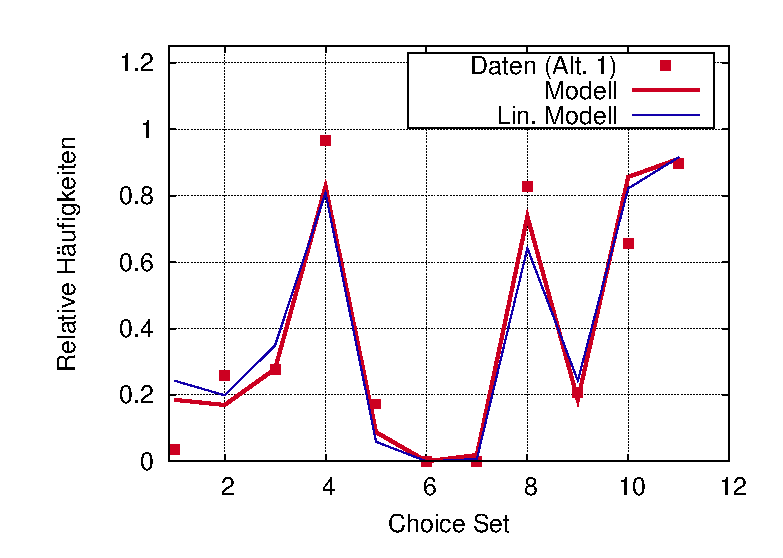
\includegraphics[width=0.49\textwidth]
   {figsDiscr/nonlinUtility_statedChoiceWS1213_fProb.eps}
 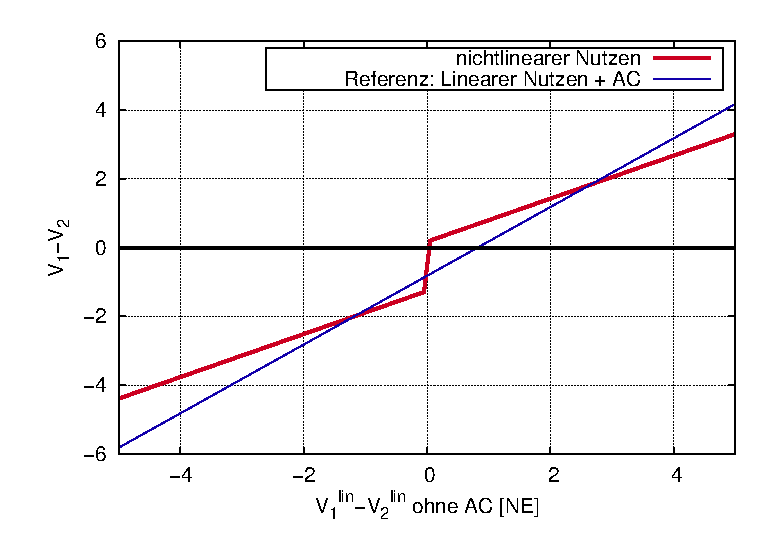
\includegraphics[width=0.49\textwidth]
   {figsDiscr/nonlinUtility_statedChoiceWS1213_Vfun.eps}
  \caption{\label{fig:mensaNl}Parametersch\"atzung des
    nichtlinearen bin\"aren Logitmodells~\refkl{mensaNl} an die
    Stated-Choice-Ergebnisse der Tabelle \emph{Mensawahl}. Links:
    Modellierungsg\"ute; rechts: Nutzendifferenz in Abh\"angigkeit der
    verrechneten linearen Nutzendifferenz.
}
\end{figure}
%###################################################

%##################################################
\begin{figure}
 \fig{0.6\textwidth}{figsDiscr/nonlinUtility_statedChoiceWS1213_lnL_beta1_beta2.eps}
  \caption{\label{fig:mensaLandscape}Ausschnitt der
    ''Optimierungslandschaft'', wenn man das
    nichtlinearen Modells~\refkl{mensaNl} anhand der
    Stated-Choice-Ergebnisse der Tabelle \emph{Mensawahl}
    sch\"atzt. Gezeigt sind die Dimensionen  
    ``lineare Zeit- und Geldsensitivit\"aten'', w\"ahrend die anderen
    drei Parameter auf die gesch\"atzten Werte gesetzt wurden.
}
\end{figure}
%###################################################

%##################################################
\begin{figure}
 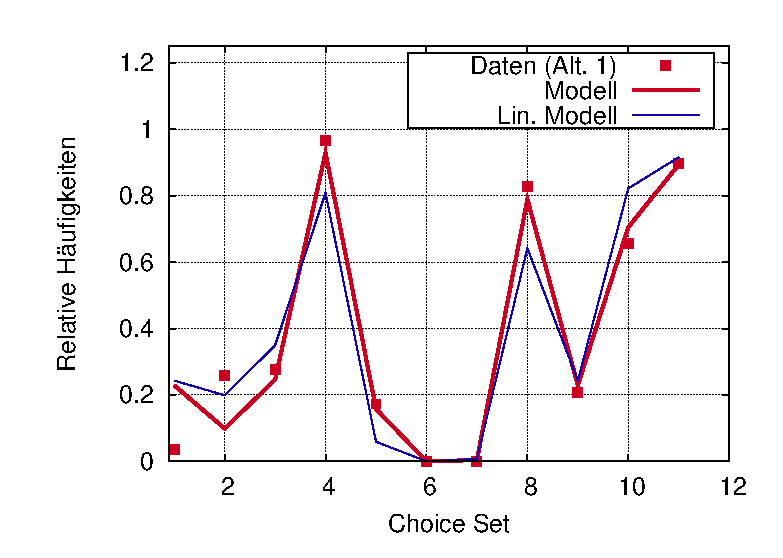
\includegraphics[width=0.49\textwidth]
   {figsDiscr/nonlinUtility_statedChoiceWS1213_quasi_fProb.eps}
 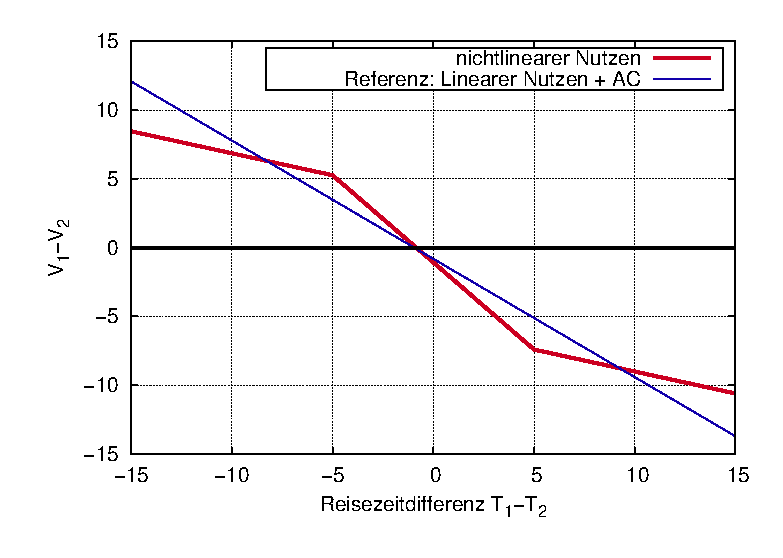
\includegraphics[width=0.49\textwidth]
   {figsDiscr/nonlinUtility_statedChoiceWS1213_quasi_Vfun.eps}
  \caption{\label{fig:mensaQuasi}Parametersch\"atzung des
    parameterlinearen bin\"aren Logitmodells~\refkl{mensaQuasi} an die
    Stated-Choice-Ergebnisse der Tabelle \emph{Mensawahl}. Links:
    Modellierungsg\"ute; rechts: Zugangszeitabh\"angigkeit der 
Nutzendifferenz bei gleichen Kosten.
}
\end{figure}
%###################################################

%##################################################
\begin{figure}
 \fig{0.95\textwidth}{figsDiscr/nonlinUtility_statedChoiceWS1213_quasi.corrMatrix.eps}
  \caption{\label{fig:mensaQuasiCorr}''Optimierungslandschaft'' der
    Log-Likelihoodfunktion  des
    parameterlinearen Logitmodells~\refkl{mensaQuasi} bez\"uglich der
    Daten der Tabelle \emph{Mensawahl}. Die jeweils nicht variierten
    Parameter wurden auf die Sch\"atzwerte gesetzt.
}
\end{figure}
%###################################################

\noindent
Abbildung~\ref{fig:mensaNl} zeigt ein Problem der
parameter-nichtlinearen Modellierung. Das beste Ergebnis, d.h. die
maximale Log-Likelihood, wird bei eigentlich unplausiblen
Parameterkombinationen erreicht. Hier ergibt sich
\bdm
M_2: \quad
\begin{array}{l}
\hatbeta_1=-0.55 \pm 0.18, \\
\hatbeta_2=-7.5 \pm 0.3, \\
\hatbeta_3=-0.54 \pm 0.03, \\
\hatbeta_4=0.7 \pm 0.2, \\
\hatbeta_5=0.002 \pm 0.509, \\
\tilL=-123.5,
\end{array}
\edm
d.h. die Breite $\beta_5$
der Nichtlinearit\"at geht gegen null, w\"ahrend die H\"ohe $\beta_4=\unit[0.7]{NE}$
endlich bleibt (vgl. rechte Grafik der Abbildung~\ref{fig:mensaNl}). Der Plot eines
Ausschnitts der ``Optimierungslandschaft'' $\tilL(\vecbeta)$,
beispielsweise bez\"uglich der linearen Geld- und Zeitsensitivit\"at
$\beta_2$ bzw. $\beta_3$ vor der nichtlinearen Bewertung
(Abb.~\ref{fig:mensaLandscape}) zeigt
zudem, dass das Optimum an einer Unstetigkeit der
``Optimierungslandschaft'' realisiert wird und damit den
``verd\"achtig'' niedrigen Standardabweichungen der zugeh\"origen
Sch\"atzer keine Bedeutung beigemessen werden darf. 

Die Sch\"atzung des parameterlinearen Modells~$M_3$, Gl.~\refkl{mensaQuasi},
an die Daten der Tabelle \emph{Mensawahl} ergibt
\bdm
M_3: \quad
\begin{array}{l}
\hatbeta_1=-1.08 \pm 0.19, \\
\hatbeta_2=-14.0 \pm 1.6, \\
\hatbeta_3=-1.27 \pm 0.16, \\
\hatbeta_4=-0.32 \pm 0.15,\\
\tilL=-119.1.
\end{array}
\edm
%
Dies sowie die Abbildungen~\ref{fig:mensaQuasi}
und~\ref{fig:mensaQuasiCorr}  zeigen, dass  die parameterlineare
Modellierung in jeder
Hinsicht zu bevorzugen ist:
\bi
\item $M_3$ enth\"alt nur vier Parameter, w\"ahrend $M_2$ f\"unf
  Parameter umfasst,
\item Die ``Fitg\"ute'' ist besser, d.h. $\tilL(\hatvecbeta)$
  gr\"o\3er,
\item Die ``Optimierungslandschaft'' um $\hatvecbeta$ ist stetig und
  differenzierbar und es ist garantiert, dass man ein globals Maximum
  erreicht hat (Abb.~\ref{fig:mensaQuasiCorr}).
\ei
Der Blick auf die rechte Grafik der Abb.~\ref{fig:mensaQuasi} zeigt,
dass, abgesehen von den ersten beiden Choice Sets, die relativen
H\"aufigkeiten vom Modell nahezu 1:1 reproduziert
werden.\footnote{Im Choice Set~1 verhalten sich die Befragten aber nicht ganz
  konsistent: In diesem Set w\"ahlt nur einer Alternative~1 w\"ahrend
  im weitgehend identischen Set~9 sechs Befragte Alternative~1 w\"ahlen.}
Insbesondere erh\"alt man signifikante Ergebnisse: Zwar ist
die Signifikanz von $\hatbeta_4$ bez\"uglich null nur marginal 
 ($p=1-\Phi(0.32/0.15) = \unit[4]{\%}$). Aber, und das ist
entscheidend, die Nullhypothese
\bdm
H_0: \beta_3=\beta_4,
\edm
oder, gleichbedeutend, die Nullhypothese
\bdm
H'_0: \text{Modell~$M_1$ beschreibt die Daten  gleich gut wie Modell~$M_3$}
\edm
kann hochsignifikant ($p<\unit[0.1]{\%}$) widerlegt werden, wie wir
mit den Mitteln des folgenden Abschnitts~\ref{sec:LR} zeigen k\"onnen.

Damit zeigt die Tabelle \emph{Mensawahl} in der Tat 
eine signifikante \emph{Erh\"ohung} der Zeitsensitivit\"ats in der N\"ahe von
$\Delta T=0$.
Der Vergleich der zwei Sensitivit\"aten $\hatbeta_3$ und $\hatbeta_4$ des
Modells $M_3$ mit der gesch\"atzten Sensitivit\"at
$\hatbeta_3\sup{M1}$ (Steigungen in Abb.~\ref{fig:mensaQuasi} rechts)
verdeutlicht diese Erh\"ohung der Sensitivit\"at anschaulich.

Als Nachteil bleibt die Ad-Hoc-Annahme der Grenzen des Intervalls
erh\"ohter Sensitivit\"at. Eine Modellierung mit $\pm 3$ oder
$\unit[\pm 7]{Minuten}$ anstelle von $\unit[\pm 5]{Minuten}$ ergab
aber \"ahnliche Ergebnisse. Wir kommen zum Ergebnis, dass, wann immer
m\"oglich, Nichtlinearit\"aten durch parameterlineare Modelle anstelle von
irreduzibel nichtlinearen Modellen formuliert werden sollten.

\verstaendnisbox{Argumentieren Sie, dass im Modell $M_3$ eine Schwellenbreite von 
$\unit[\pm 10]{Minuten}$ dieses Modell auf $M_1$ reduzieren w\"urden,
  wenn man es auf die Tabelle \emph{Mensawahl} 
  anwendete: Die Sch\"atzer f\"ur $\beta_1$ bis $\beta_3$ w\"aren dann
  gleich, w\"ahrend $\beta_4$ nicht mehr gesch\"atzt werden kann, so dass
  das Modell bez\"uglich dieser Daten fehlspezifiziert w\"are.}

\verstaendnisbox{Gibt es in der Tabelle \emph{Mensawahl} ein
  Choice Set mit einer dominanten Alternative? Wenn ja, welches?}

 
%##################################
\section{\label{sec:LR}Modellvergleich: Likelihood-Ratio-Test}
%##################################

\providecommand{\Mr}{\text{M}\sup{(r)}}

Bei den Regressionsmodelle hatten wir den F-Test und den $T^2$-Test zur Bestimmung der
Relevanz von exogenen Variablen und zugeh\"origer Modellparameter
kennengelernt. Die Frage war: Erkl\"art der bzw. die zus\"atzliche(n)
Parameter des komplizierteren Modells den Sachverhalt signifikant besser als 
ein einfacheres Modell ohne diese Parameter, oder wird das Modell
durch die zus\"atzlichen Parameter fehlspezifiziert? Bei 
Modellen der diskreten Wahltheorie \"ubernimmt diese wichtige Aufgabe
der \bfdef{Modellspezifikation}  der
\emph{Likelihood-Ratio-Test} (LR-Test).\footnote{Manchmal wird zwischen
``Likelihood-Ratio-Test'' und ``Maximum Likelihood-Ratio-Test''
unterschieden: Der Likelihood-Ratio-Test vergleicht das gesch\"atzte
volle Modell
gegen das \emph{nicht} gesch\"atzte Trivialmodell (z.B. ``alle
Wahrscheinlichkeiten sind gleich''), w\"ahrend der Maximum
Likelihood-Ratio-Test zwei gesch\"atzte verschachtelter Modelle vergleicht.
In dieser Diktion w\"urde hier der ``Maximum Likelihood-Ratio-Test'' vorgestellt.
Dies ist aber spitzfindig, da es beim Trivialmodell nichts zu sch\"atzen
gibt und es deshalb auch als ``gesch\"atztes Modell'' durchgehen
w\"urde. Insbesondere ist die technische Durchf\"uhrung des Tests immer
gleich.}

Der LR-Test ist zum Vergleich zweier \emph{verschachtelter} Modelle
anwendbar, das hei\3t, das einfachere oder \bfdef{restringierte}
Modell $\Mr$ mit $M_r$ Parametern ist im komplexeren \bfdef{unrestringierten} Modell~M
 mit $M>M_r$ Parametern enthalten. Im letzten Abschnitt \"uber
 nichtlineare Nutzenfunktionen sind beispielsweise die Modelle $M_1$,
 $M_2$ und $M_4$, nicht jedoch $M_3$, restringierte Modelle bez\"uglich des
 durch~\refkl{V-nichtlin1} beschriebenen vollen nichtlinearen Modells. 

\bi
\item Typischerweise werden im restringierten Modell einige Parameter
des unrestrin\-gier\-ten Modells auf feste Werte, h\"aufig auf null,
gesetzt (daher der Name ``restringiert'' = ein\-ge\-schr\"ankt).
\item Setzt man alle Parameter=0, erh\"alt man das
\bfdef{Trivialmodell}: Bei quasilinearen stetigen Modellen (Regressionsmodellen)
lautet dieses $\hat{y}=0$ und bei diskreten Wahlmodellen mit $I$ Alternativen
$V_{ni}=0$ bzw. $P_{ni}=1/I$.
\item Eine weitere Variante von Einfachstmodellen ist das
\bfdef{Konstantenmodell}: Bei den quasilinearen Regressionsmodellen
lautet diese $\hat{y}=\beta_0$ mit dem LSE oder ML-Sch\"atzer
$\hatbeta_0=\bar{y}$. Bei diskreten Wahlmodellen mit $I$ Alternativen
entspricht dies der Nutzenfunktion (siehe Abschnitt~\ref{sec:konstantenmodell})
\be
\label{konstantenmodell1}
V_{ni}=\sum_{j=1}^{I-1}\beta_j\delta_{ji},
\ee
die einen kompletten Satz von alternativenspezifischen Konstanten (ACs)
repr\"asen\-tiert, und das nach der ML-Methode gesch\"atzte Modell
f\"uhrt sowohl bei 
Logit- als auch bei Probitmodellen zu den Auswahlwahrscheinlichkeiten
$P_{ni}=f_i$ (Wahrscheinlichkeiten gleich den beobachteten relativen
H\"aufigkeiten), unabh\"angig von der Wahlentscheidung $n$ (siehe Abschnitt~\ref{sec:konstantenmodell}).
\ei

%########
\subsection{Vorgehen}
%########

Wie der Name schon sagt, wird beim LR-Test zum Bilden der Testvariable
das
Verh\"altnis der Likelihood-Werte der gesch\"atzten Modelle, genauer der
Logarithmus davon, verwendet: Das Vorgehen ist analog zu den sonstigen
Tests:
\benum
\item \bfblack{Nullhypothese $H_0$:} Die zus\"atzlichen Parameter des
unrestringierten Modells sind irrelevant, tragen also nichts zur
Erkl\"arung des Sachverhalts bei

\item  \bfblack{Test-Statistik:} 
Die Test-Variable $\lambda\sup{LR}$ (logarithmiertes Likeli\-hood-Ratio)
\maineq{LRtest}{
\lambda\sup{LR}=2\ln\left(
  \frac{L\left(\hatvecbeta\right)}{L\sup{r}\left(\hatvecbeta\sup{r}\right)}\right)
=2\left[
  \tilL\left(\hatvecbeta\right) 
 - \tilL\sup{r}\left(\hatvecbeta\sup{r}\right)
\right]
\sim \chi^2(M-M_r).
}
%
gehorcht bei G\"ultigkeit der Nullhypothese \emph{asymptotisch} einer
$\chi^2$-Verteilung mit  $M-M_r$ Freiheitsgraden: Pro zus\"atzlichen
Parameter (Parameterzahl $M$) des unrestringierten Modells ein
Freiheitsgrad. 

\item \bfblack{Bestimmung der Realisierung $\lambda\sup{LR}\sub{data}$ von $\lambda\sup{LR}$}: Diese
f\"allt als Nebenprodukt der ML-Sch\"atzung automatisch mit ab. Hat
das Modell~M nur zwei Parameter, 
kann man $\lambda\sup{LR}\sub{data}$ auch direkt aus dem Plot der Log-Likelihood
ablesen (vgl. das Beispiel auf S.~\pageref{bspLRGraph} und
die Aufgabe auf S.~\pageref{aufg:topDown}).

\item \bfblack{Testergebnis}: 
\bi
\item Entweder klassisch mit einer vorgegebenen
Fehlerwahrscheinlichkeit: $H_0$ wird bei einer
Fehlerwahrscheinlichkeit $\alpha$ abgelehnt, d.h das unrestringierte
Modell beschreibt die Daten signifikant besser als das restringierte,
falls f\"ur die Realisierung gilt
\be
\label{LRergebnis}
\lambda\sup{LR}\sub{data}>\chi^2_{1-\alpha, M-M_r},
\ee

\item oder direkt mit dem $p$-Wert: Bei Zutreffen von $H_0$ erh\"alt
man nur mit der Wahrscheinlichkeit
\be
\label{LRpWert}
p=1-F_{\chi^2}^{(M-M_r)} \big(\lambda\sup{LR}\sub{data} \big)
\ee
gr\"o\3ere $\lambda\sup{LR}$-Werte als $\lambda\sup{LR}\sub{data}$. Wie bei den
Regressionsmodellen stellt der $p$-Wert die minimale
Fehlerwahrscheinlichkeit dar, bei der $H_0$ gerade noch abgelehnt
werden kann.
\ei
\eenum
Im Gegensatz zu den $T^2$ und $F$-Tests  der Regressionsmodelle ist
der LR-Test nur ``asymptotisch'' g\"ultig, da nur dann $\lambda\sup{LR}$ einer
$\chi^2$-Verteilung gehorcht.
``Asymptotisch'' hei\3t, dass die zur exakten
Reproduktion der Daten durch das Modell ben\"otigte Information die
Parameterzahl bei weitem \"ubersteigt, so dass Fehler beim Sch\"atzen
der Varianz-Kovarianzmatrix vernachl\"assigbar werden. Dies entspricht
in der Regressionsrechnung Tests bei bekannter Varianz: Beim $T$-Test geht
die Student-t-Verteilung in eine
Standardnormalverteilung \"uber, beim $T^2$-Test (als Spezialfall
eines $F$-Tests f\"ur eine Parameterzahldifferenz von 1) in eine
$\chi^2(1)$-Verteilung. Konsistent dazu 
 unterscheidet sich bei hinreichend hohem Datenumfang
die Likelihoodfunktion an
allen relevanten Stellen nur unwesentlich von der 
 multivariaten Gau\3verteilung, siehe Abschnitt~\ref{sec:discr-covar},
 insbesondere Gl.~\refkl{Lgauss}. 

\emph{Aufgabe $T^2$ Test einbauen!}
 
%!!!Dies wird in einer
%\myHyperlink{http:/www.mtreiber.de/Vkoek_Ma/download/aufg09.pdf}{\"Ubungsaufgabe}
%n\"aher diskutiert.
%~/vorlesungen/Verkehrsoekonometrie_Ma_AufgSamml/discreteChoice/LRtestStetig

 
\subsubsection{Beispiel}
\label{bspLRGraph}
Betrachtet wird eine auf zwei Alternativen aggregierte
Revealed-Choice-Befragung wie in
Abschnitt~\ref{sec:revealedChoiceEntf} und eine Modellierung durch das
dort ausf\"uhrlich diskutierte 
 binomiale Logit-Model mit den deterministischen Nutzenfunktion
\bdm
V_{ni}(x) =(\beta_1r_i+\beta_2)\delta_{i1}
\edm
mit der 
Wegl\"ange $r$ als einziger
 exogener Faktor, nur dass hier die Daten nur
einer Vorlesungsbefragung herangezogen werden. Aufgrund der
kleineren Fallzahlen sind die Parametersach\"atzer nicht so hoch
signifikant wie dort und die Auswertung interessanter.  

Abbildung~\ref{fig:BNL_kalib_logL-LRTest} zeigt die Log-Likelihood daf\"ur, dass das
Modell genau die Daten der Tabelle~\ref{tab:revealedChoiceBin} liefert. LR-Tests
lassen sich hier einfach graphisch durchf\"uhren 
(H\"ohenlinien\-ab\-stand 1, maximale Log-Likelihood $-26.2$,
``h\"ochste'' H\"ohenlinie bei $\tilL=\ln L=-27$)
 
%#######################################
\begin{figure}
\fig{0.7\textwidth}{figsDiscr/BNL_kalib_logL.eps}
\caption{\label{fig:BNL_kalib_logL-LRTest}Log-Likelihood des
  gerechneten Beispiels zum LR-Test.}
\end{figure}
%#######################################


\paragraph{Test 1: Ist die Entfernung ein signifikanter Einflussfaktor?}
\benum
\item Nullhypothese $H_0$: Die Entfernung ist nicht relevant, dass
  restringierte Modell $\Mr$: $V_{ni}=\beta_2\delta_{i1}$ beschreibt die Daten nicht
  schlechter bzw. $\beta_1=0$.

\item Test-Statistik: Da das volle Modell~M zwei Parameter und das
  restringierte einen Parameter enth\"alt, ist
\bdm
\lambda\sup{LR}=2\left[
  \tilL(\hatbeta_1,\hatbeta_2)-\tilL\sup{r}(\hatbeta_2\sup{r})
 \right] \sim \chi^2(1).
\edm
\item Realisierung von $\lambda\sup{LR}$ aus den Daten bzw. der
  Log-Likelihood-Funktion:
\bi
\item Das volle Modell wird durch $\hatbeta_1=-0.35$ und $\hatbeta_2=1$
gesch\"atzt. Die zugeh\"orige Log-Likelihood ist laut Angabe
$\tilL(\hatbeta_1,\hatbeta_2)=-26.2$.
\item Zur Sch\"atzung des restringierten Modells wird die Log-Likelihood auf der
Linie $\beta_1=0$ (der Restriktion) bez\"uglich $\beta_2$ maximiert. Dies
ergibt $\hatbeta_2\sup{r}=-0.5$ und die dazugeh\"orige Log-Likelihood 
$\tilL\sup{r}(\hatbeta_2\sup{r})$ von $-32$ (einfach die H\"ohenlinien z\"ahlen)
\ei
Damit 
\bdm
\lambda\sup{LR}=2(-26.2+32)=11.6
\edm

%######################
\begin{figure}
\fig{0.7\textwidth}{figsDiscr/chi2_F.eps}
\caption{\label{fig:chi2}Verteilungsfunktion der $\chi^2(m)$ Verteilung f\"ur
  verschiedene Freiheitsgrad-Zahlen $m$.}
\end{figure}
%######################

\item Entscheidung: Hier wird die Realisierung mit der Verteilungsfunktion der
  $\chi^2(1)$-Verteilung verglichen (vgl. Abb.~\ref{fig:chi2}).
Dabei liegt 11.6 schon au\3erhalb des Darstellungsbereichs der Grafik. Aber
selbst bei $\lambda\sup{LR}=10$ ist die Kurve f\"ur einen Freiheitsgrad schon oberhalb
0.99. Also
\bdm
F_{\chi^2}^{(1)}(11.6)>0.99 \ \Rightarrow \ p<\unit[1]{\%}
\edm
Der $p$-Wert ist also kleiner als \unit[1]{\%} (er ist sogar kleiner als 1
Promille), also ist die Entfernung ein wichtiger Einflussfaktor und der
zugeh\"orige Parameter $\beta_1$ hochisgnifikant von null verschieden.
Der LR-Test geht also zugunsten des vollen Modells~M aus.
\eenum

\paragraph{Test 2: Ist die globale Bevorzugung (alternativenspezifische
  Konstante)  ein signifikanter Einflussfaktor?}
\benum
\item Nullhypothese $H_0$: Die Bevorzugung  ist nicht relevant und das
  restringierte Modell $\Mr$: $V_{ni}(x)=\beta_1x\delta_{i1}$ 
beschreibt die Daten nicht
  schlechter als das volle Modell. Anders ausgedr\"uckt: $\beta_2=0$.

\item Test-Statistik: Wie beim Test 1
 
\item Realisierung von $\lambda\sup{LR}$:
\bi
\item Das volle Modell wurde bereits beim Test 1 gesch\"atzt: 
$\hatbeta_1=-0.35$, $\hatbeta_2=1$ und $\tilL(\hatbeta_1,\hatbeta_2)=-26.2$.
\item Zur Sch\"atzung des restringierten Modells wird die Log-Likelihood auf der
Linie $\beta_2=0$ bez\"uglich $\beta_1$ maximiert. Dies
ergibt $\hatbeta_1\sup{r}=-0.17$ und die dazugeh\"orige Log-Likelihood 
$\tilL\sup{r}(\hatbeta_2\sup{r})$ von $-27.7$ (das Maximum ist deutlich
n\"aher an der H\"ohenlinie $\tilL=-28$ als an der Linie $\tilL=-27$). 
\ei
Damit 
\bdm
\lambda\sup{LR}=2(-26.2+27.8)=3.2
\edm

\item Entscheidung: Hier wird die Realisierung mit der Verteilungsfunktion der
  $\chi^2(1)$-Verteilung verglichen (vgl. Abb.~\ref{fig:chi2}).
Es gilt 
\bdm
F_{\chi^2}^{(1)}(3.2)\approx 0.92 \ \Rightarrow \ p=\unit[8]{\%}
\edm
Der $p$-Wert ist also \unit[8]{\%}, was in der Regel nicht mehr als
signifikant betrachtet wird. L\"asst man z.B. eine Fehlerwahrscheinlichkeit
$\alpha=\unit[5]{\%}$ zu und liest aus der Grafik das Quantil
$\chi^2_{1-\alpha,1}=4$ ab, so ist die Realisierung $\lambda\sup{LR}$ kleiner als das
Quantil, der Test also nicht widerlegbar. Per Definition ist die geringste
Fehlerwahrscheinlichkeit, bei der $H_0$ gerade noch widerlegbar ist, gleich
$p=\unit[8]{\%}$. 

Der LR-Test geht bei \unit[10]{\%} Fehlerwahrscheinlichkeit
zugunsten des Vollen Modells~M, bei \unit[5]{\%} Fehlerwahrscheinlichkeit
zugunsten des restringierten Modells $\Mr$. Der Einfluss der
globalen Bevorzugung ist also grenzwertig. Generell sollte man beim LR-Test im
Zweifelsfall das komplexere Modell beibehalten und erst bei $p$-Werten oberhalb von
\unit[10]{\%} das einfachere in Betracht ziehen.  
\eenum

\aufgabenbox{Verst\"andnisaufgabe:}{Wie ist es zu erkl\"aren, dass im
  restringierten Modell
  $\Mr$ (vgl. den Test 1) $\beta_2\sup{r}<\beta_2$, 
der globale Bonus der Alternative 1
  (Fu\3/Rad) gegen\"uber dem vollen Modell wesentlich kleiner ist (insbesondere
  negativ statt positiv)? Warum ist beim restringierten Modell
  $\Mr$ des Tests 2 $\beta_1\sup{r}>\beta_1$, die Zeitbewertung
  der ``langsameren'' Verkehrsmittel also nicht ganz so negativ wie beim
  vollen Modell~M}
\vspace{-1.5em}

{\scriptsize Da das (bez\"uglich de rrelevanten Faktoren) 
fehlspezifizierte Modell $\Mr$ keine Zeitbewertung
  enth\"alt, muss die offensichtliche Unattraktivit\"at der langsameren Modi 
bei gro\3en Entfernungen
  \"uber den einzig verbleibenden Freiheitsgrad der globalen Bewertung
  modelliert werden. Diese wird dadurch negativ ($\beta_2\sup{r}<0$), obwohl eigentlich Fu\3/Rad
  gegen\"uber \"OV/MIV bei \emph{ceteris-paribus} Bedingungen einen Bonus
  $\beta_2>0$ besitzen. Analog wird im Modell $\tilde{M}\sup{r}$ die fehlende
  M\"oglichkeit der Ber\"ucksichtigung einer globalen Bevorzugung der
  langsameren Verkehrsmittel \"uber eine entsprechend weniger negative
  Entfernungsbewertung ``verrechnet''.
}


%###################################################
\begin{figure}[t!]
\vspace{-2em}  
  \fig{0.9\textwidth}{./figsDiscr/BNL_kalib_L.eps}
 \vspace{-4em}  
  \caption{\label{fig:BNL_kalib_L}Der Quotient
$L(\beta_1,\beta_2)/L\sub{max}$, welcher direkt proportional zur zweidimensionalen
Dichtefunktion der tats\"achlichen Parameterwerte ist. Die
Konfidenzregion des Likelihood-Ratio-Test bez\"uglich des
Trivialmodells $V_{ni}=0$ zur Fehlerwahrscheinlichkeit
$\alpha=\unit[5]{\%}$ ist dick umrandet. Der Rand entspricht einer
Log-Likelihood-Differenz von $\frac{1}{2} \, \chi^2_{2,1-\alpha}\approx 3$, also 
$L(\beta_1,\beta_2)/L\sub{max}=e^{-3}$.
}
\end{figure}
%###################################################


\subsection{Test auf Relevanz der Einflussfaktoren mit dem Top-Down-Ansatz}
Eine der wichtigsten Anwendungen ist die Eliminierung irrelevanter
Parameter, da sonst das Modell nicht korrekt spezifiziert ist. Dabei
kann man z.B. nach folgenden Top-Down-Ansatz vorgehen:
\bi
\item Man stellt ein
komplexes Modell~M auf, welches alle Einflussfaktoren
enth\"alt, welche aufgrund der Daten messbar sind und die man aufgrund theoretischer
\"Uberlegungen f\"ur sinnvoll h\"alt. 
\item Dieses Modell wird
nacheinander mit restringierten Modellen verglichen, bei
denen jeweils ein Parameter =0 (oder auf einen aus theoretischen
\"Uberlegungen kommenden festen Wert)  gesetzt wird. 
\item Der Parameter
mit dem h\"ochsten $p$-Wert wird gestrichen und das resultierende
Modell wird das neue unrestringierte Modell. 
\item Das Verfahren wird so lange
fortgesetzt, bis kein Parameter mehr $p$-Werte oberhalb von
z.B. $\alpha=\unit[5]{\%}$ hat.
\ei
Dabei muss man allerdings auf Abh\"angigkeiten achten, da die
Signifikanz eines Parameters durchaus von der Existenz anderer
Parameter abh\"angt und im Extremfall eine Gruppe von
Einflussfaktoren relevant sein kann, auch wenn es jeder einzelne nicht
ist. Dies wird gepr\"uft, indem man einen LR-Modellvergleich  des
durch die Top-Down-Methode resultierenden
Modells mit dem urspr\"unglichen ``komplexen'' Ausgangsmodell durchf\"uhrt.



\aufgabenbox{\label{aufg:topDown}Aufgabe: Top-Down-Ansatz}{Testen Sie die Relevanz beider
Parameter der Binomial-Logit und Probitmodelle mit deterministischen
Nutzenfunktionen gem\"a\3~\refkl{binomBeisp1} 
bei der Beschreibung der  in Tabelle~\ref{tab:binomBeisp1} angegebenen
Daten. F\"uhren Sie den Likelihood-Ratio-Test graphisch anhand 
Abb.~\ref{fig:logLbinom} durch.}

\aufgabenbox{Aufgabe: Trivialmodelle}{Zeigen Sie, dass die
Auswahlwahrscheinlichkeiten der Trivialmodelle der diskreten
Wahlmodelle $(V_{ni}=0$) durch $P_{ni}=1/I$ gegeben sind.
}

\aufgabenbox{Aufgabe: Konstantenmodelle}{Zeigen Sie f\"ur das multinomiale Logit und
Probit-Modell, 
dass die ML-Sch\"atzung
der Konstantenmodelle~\refkl{konstantenmodell} der diskreten
Wahltheorie zu Auswahlwahrscheinlichkeiten gleich den relativen
H\"aufigkeiten f\"uhrt. 

\emph{Hinweis:} Betrachten Sie die Wahrscheinlichkeiten direkt.
}
%
%\aufgabenbox{Aufgabe: $\chi^2$ Verteilung der Test-Statistik}{Zeigen
%Sie, dass bei Regressionsmodellen mit unbestimmten Anteilen gem\"a\3
%den Gau\3-Markow-Annahmen ein Vergleich des gesch\"atzten
%Konstantenmodells $\hat{y}=\bar{y}$ mit dem Trivialmodell $\hat{y}=\mu_0$
%eine exakt $\chi^2(1)$-verteilte LR-Statistik $\lambda\sup{LR}$ liefert, wenn
%$H_0$ zutrifft, also $\mu=E(Y)=\mu_0$.
%
%\emph{Hinweis:} quadrierte standardnormalverteilte Zufallsvariablen
%sind $\chi^2(1)$-verteilt. Siehe auch
%\myHyperlink{http:/www.mtreiber.de/Vkoek_Ma/download/aufg09.pdf}{diese
%\"Ubungsaufgabe}.
%}


%##################################
\section{\label{sec:gueteDiscr}Modellqualit\"at: Goodness-of-Fit Ma\3e}
%##################################

%\red{Einfuegen neues Material: Horowitz-Test: vkoek-Teil4-HorowitzTest.README}

Der LR-Test eignet sich gut zur Eliminierung \"uberfl\"ussiger
Parameter und den Testen einzelner neuer Einflussfaktoren auf
Signifikanz. Die z.B. nach einer Top-Down Elimination  verbleibenden
Variablen sind notwendig, aber ggf. nicht hinreichend f\"ur eine
korrekte Modellspezifikation. Als Indiz, ob man noch wichtige
Einflussfaktoren \"ubersehen hat,\footnote{Faktoren aufzusp\"uren ist
sehr viel schwieriger als welche zu eliminieren, da man nicht wei\3, nach was
man suchen soll!} kann der Vergleich des Modells mit
dem entsprechenden \emph{Konstantenmodell} dienen.\footnote{Der
Vergleich mit dem Trivialmodell kann bei Alternativen mit sehr
geringen empirischen relativen
H\"aufigkeiten irref\"uhrend sein, da dann das -- eigentlich auch
triviale -- Konstantenmodell oft mehr erkl\"art als alle weiteren
Parameter des vollen Modells.}
Dabei sollte sich nicht nur Signifikanz beim LR-Test ergeben, sondern
auch das Modell als solches eine hohe G\"ute haben.\footnote{Der LR-Test sagt
nur aus, ob ein Modell signifikant besser als ein anderes ist, aber
nichts \"uber die absolute G\"ute: Besser ist nicht immer gut!}.

Eine weitere Problemstellung, bei der der LR-Test nicht weiterhelfen
kann, ist der Qualit\"atsvergleich zweier \emph{nichtverschachtelter}
Modelle: Welches ist besser und ist der Unterschied signifikant? Man
ben\"otigt also ein absolutes Ma\3 f\"ur die G\"ute eines
Modells. Mehrerer solcher Ma\3e wurden vorgeschlagen und in der
\"ublichen Statistik-Software implementiert ($M$ bezeichnet die Zahl der zu
sch\"atzenden Parameter und $n$ die Zahl der Beobachtungen,
$\tilL=\ln L$ die Log-Likelihood des kalibrierten Modells):


\bi
\item \bfdef{Akaike's information criterion}:
  \be \text{AIC}=-2\tilL+2M\frac{n}{n-(M+1)} \ee

\item \bfdef{Bayesian information criterion:}
   \be \text{BIC}=-2\tilL+M\ln n \ee

\item \bfdef{LR-Index} bzw. \bfdef{McFaddens R$2$}:
   \be \rho^2=1-\frac{\tilL}{\tilL\sup{0}} \ee
 
\item \bfdef{korrigierter LR-Index} bzw. \bfdef{adjusted
  likelihood-ratio index} bzw. \bfdef{McFaddens
  korrigiertes R$2$}:
  \be \bar{\rho}^2=1-\frac{\tilL-M}{\tilL\sup{0}}\ee
\ei
   
Dabei ist $\tilL\sup{0}$ die Log-Likelihood des Konstantenmodells
oder, falls man das G\"utema\3 schw\"acher formulieren will, des
Trivialmodells.\footnote{Dies ist 
analog wie bei der G\"utemessung der Wettervorhersage: Das
Trivialmodell w\"are z.B. ``Das Wetter wird sch\"on'' und das
Konstantenmodell ``Das Wetter \"andert sich nicht''.}
Folgende Aussagen gelten bez\"uglich dieser Kenngr\"o\3en:

\bi
\item Die beiden Informationskriterien geben die Information in Bit
  an, die man im Mittel \emph{zus\"atzlich} ben\"otigt, um von der
  Modellvoraussage zu den tats\"achlichen Mikrodaten,
  d.h. den tats\"achlich getroffenen Entscheidungen, zu kommen. Die
  beiden Kriterien haben geringf\"ugig andere Annahmen bei der Herleitung,
  deshalb die unterschidliche Form.

\item Zur Modellauswahl kann man sowohl das AIC als auch das BIC
  heranziehen: Je niedriger, desto besser. Das BIC legt einen
  st\"arkeren Fokus auf parameter-sparsame (\emph{parsimonious})
  Modelle.

\item Bei verschachtelten Modellen, welche der Nullhypothese des
  LR-Tests gen\"ugen, ist bei hinreichend viele Beobachtungen
  ($n\gg  M$) der Erwartungswert des AIC
    gleich. Insbesondere entspricht das Ereignis ``das erweiterte
    Modell hat ein kleineres AIC'' einem $p$-Wert des LR-Tests
    $<0.5$. Insofern entspricht das AIC dem LR-Test, ist aber auch auf
    nichtverschachtelte Modelle anwendbar. 

  \item Ein weiterer Test der Nullhypothese gleicher G\"ute zweier
    nichtverschachtelter Modelle ist der
    \bfdef{Horowitz-Test}. Dieser wird hier aber nicht weiter
    behandelt.
    
\item Der LR-Index bzw. der korrigierte LR-Index 
entspricht dem Bestimmtheitsma\3
$R^2=B=1-U$, Gl.~\refkl{Bmass},
bzw. dem korrigierten Bestimmtheitsma\3 $\bar{R}^2$,
Gl~\refkl{BmassKorr},  quasistetiger Regressionsmodelle, daher auch
der Name ``(korrigierter) McFadden R$^2$'': 
 W\"ahrend $R^2$ den erkl\"arten Anteil der beobachteten Variation
beschreibt, entspricht $\rho^2$ dem erkl\"arten Anteil der zur exakten
Reproduktion der Daten n\"otigen Log-Likelihood, wenn man vom
Trivial- bzw. Konstantenmodell ausgeht. $\tilL/\tilL_0$ entspricht
dann dem Anteil der nichterkl\"arten Log-Likelihood. Im Sinne der
Shannon'schen Definition entspricht  $\rho^2$ und auch $R^2$
 dem erkl\"arten Anteil der in den Daten
 enthaltenen Informationsmenge.
 \item Die ``korrigierten'' Gr\"o\3en $\bar{R}^2$ und $\bar{\rho}^2$
   ber\"ucksichtigen den ``Verbrauch'' von Daten bei der Fit-Prozedur
   und korrigieren die Tendenz zum \"Uberfitten, falls $n$ nicht
   $\gg M$ ist. Insbesondere liefert ein beliebig schlechtes Modell
mit $M$ Parametern, welches $M$ Beobachtungen erkl\"aren soll, nach der
Kalibrierung eine perfekte \"Ubereinstimmung mit den Daten, 
also $R^2=1$ bz. $\rho^2=1$, w\"ahrend $\bar{R}^2$ und $\bar{\rho}^2$
dann in der N\"ahe von Null oder undefiniert sind.
 \item Der korrigierte Likelihood-Ratio
Index (korrigiertes McFadden R$^2$) $\bar{\rho}^2$ kann sowohl zur Modellauswahl (je
h\"oher, desto besser), also auch zur absoluten G\"utebestimmung eines
Modells angewandt werden. Die \emph{Beurteilung} der \emph{G\"ute} ist
jedoch bei $\bar{R}^2$ und $\bar{\rho}^2$ konzeptionell unterschiedlich: Aufgrund der
inh\"arenten Stochastizit\"at hat selbst ein perfektes Auswahlmodell
einen deutlich von 1 verschiedenen $\rho^2$-Wert (siehe Beispiel
weiter unten).

\item Hat bei der Kalibrierung zweier verschachtelter Modelle mit
vielen Daten ($n\gg  M$) das erweiterte Modell ein ``besseres''
(h\"oheres) $\rho^2$, entspricht das $p<0.5$ beim LR-Test. Dies
macht die Eignung von $\rho^2$ zur Modellauswahl allgemeiner,
auch nichtverschachtelter Modelle plausibel.

\ei


\examplebox{Beispiel: Zwei Alternativen, nur das Geschlecht ist
  relevant}
{Ist bei einer
binomialen Wahlsituation f\"ur Frauen die beobachtete relative H\"aufigkeit, Alternative~1
zu w\"ahlen, =0.1, und f\"ur M\"anner=0.9, sind au\3erdem alle anderen
Einflussfaktoren bei allen Personen gleich, so kann das beste Modell
nicht besser sein, als f\"ur Frauen $P_{n1}=0.1$ und $P_{n2}=0.9$
vorauszusagen (und bei M\"annern umgekehrt). Dadurch
erniedrigt sich die Log-Likelihood bei jeder 
Wahlentscheidung $n$ (egal ob Mann oder Frau)  \emph{im Mittel} um 
\bdm
\Delta \tilL_n=\sum_iy_{ni}\ln P_{ni}=0.1 \ln 0.1+0.9\ln 0.9=-0.325
\edm
w\"ahrend im Nullmodell ($P_{ni}=1/2$) die mittlere \"Anderung pro Entscheidung
durch
\bdm
\Delta \tilL_n^{(0)}=\sum_iy_{ni}\ln P_{ni}=0.1 \ln 0.5+0.9\ln 0.5=\ln
0.5=-0.693
\edm
gegeben ist. Damit hat in dieser Situation
 selbst das beste Modell nur einen $\rho^2$-Wert
von 
\bdm
\rho^2=1-\frac{\tilL-M}{\tilL\sup{0}}=0.531.
\edm
}
\maintext{Aufgrund der Stochastizit\"at der modellierten endogenen Variablen
kann selbst das ``beste'' Modell die Mikro-Information nicht auch nur
ann\"ahernd reproduzieren. Deshalb sind, je nach den beobachteten
relativen H\"aufigkeiten, $\rho^2$-Werte von 0.5 meist schon sehr gut,
w\"ahrend $R^2=0.5$ ein ziemlich schlechtes Regressionsmodell charakterisiert.}

\emph{Achtung:} Als absolute Ma\3e sind die
Likelihood-Ratio-Indices durch
\emph{Quotienten} der Log-Likelihood formuliert, nicht durch \emph{Differenzen} wie
bei der Parametersch\"atzung oder der Testvariablen des LR-Tests. 
Fasst man $y_n>1$ Beobachtungen zu Klassen $n$ zusammen, m\"ussen die
sonst irrelevanten 
Multinomialkoeffizienten der Likelihoodfunktion
ber\"ucksichtigt werden.

\newpage
%#######################################
\section{\label{sec:GEV}Generalized-Extreme-Value (GEV) Modelle} 
%#######################################

%\EinsteinBeg

Die Modellklasse der Generalized-Extreme-Value Modelle (GEV Modelle)
wurde von McFadden (1978) mit der Intention entwickelt, unter
Beibehaltung der analytischen Berechnenbarkeit der
Auswahlwahrscheinlichkeiten m\"oglichst reichhaltige
Korrelationsstrukturen zwischen den Alternativen zuzulassen.  



%#######################################
\subsection{Motivation}
%#######################################

Bei Entscheidungssituationen sind h\"aufig mehrere
Einzelentscheidungen so miteinander gekoppelt, dass sie
sinnvollerweise nur gemeinsam
modelliert werden k\"onnen. Beispiele der Verkehrs\"okonometrie sind
\bi
\item \emph{T\"agliche Entscheidung von Einzelpersonen}:
Zielwahl und Verkehrsmittelwahl, oder noch allgemeiner,
Aktivit\"aten-, Ziel-, Verkehrsmittel- und Routenwahl. Insbesondere
h\"angen die Ziel- und Verkehrsmittelwahl miteinander zusammen, da
entferntere Ziele nur mit den ``schnellen'' Verkehrsmodi \"OPNV und
MIV sinnvoll zu erreichen sind.
\item \emph{Langfristige Entscheidungen von Einzelpersonen oder
Haushalten}: 
Wohnort- und Arbeitsplatzwahl: Es w\"are unklug, den Wohnort
ohne Ber\"ucksichtigung des zu\-k\"unf\-ti\-gen Arbeitsplatzes oder den
Arbeitsplatz ohne Ber\"ucksichtigung des Wohnortes auszuw\"ahlen.
\item \emph{Planungsentscheidung eines \"OPNV-Betriebs}:
Auswahl einer Variante des zu\-k\"unf\-ti\-gen Fahrplans und ggf. Kauf neuer
Bahnen+Busse
\item \emph{Investitionsentscheidungen bei der Expansion einer Firma}:
Neue Zweigstelle Ja / Nein? Ggf. Wahl der Region und des konkreten Ortes
der neuen Zweigstelle.
\ei
Im einfachsten Fall fasst man alle Varianten der komplexen
Entscheidung kombinatorisch zu einzelnen Alternativen zusammen und
wendet die bisherigen Modelle, vorzugsweise das MNL-Modell,
an. Bei einer Einkaufsentscheidung  k\"onnte  man bei diesem Vorgehen 
beispielsweise eine Alternativenmenge der Form 
\be
\label{nestedLogit-A}
A=\{\text{(E,\"OV), (E,MIV), (D,\"OV), (D,MIV)} \}
\ee
(E f\"ur ``Tante-Emma-Laden'' und D f\"ur ``Discounter'') bekommen
(vgl. Abb.~\ref{fig:NL-Beispiel} im Beispiel weiter unten).

Allerdings liegt es in der Natur geschachtelter Entscheidungen, dass
die Zufallsnutzen, entgegen der bisherigen Modellspezifikation, nicht
unabh\"angig voneinander sind. Beispielsweise haben die Alternativen 
$A_1=\text{(E,\"OV)}$ und $A_2=\text{(E,MIV)}$ den Ladentyp
``Tante-Emma-Laden'' als
gemeinsames Merkmal  und damit gemeiname Zufallsnutzenkomponenten,
n\"amlich alle dem Ladentyp zuzuordnenden Anteile des
Zufallsnutzens. Damit sind f\"ur jede Person $n$ die Zufallsnutzen $\epsilon\sub{E,\"OV}$ und
$\epsilon\sub{E,MIV}$ positiv korreliert. Die Modellierung von
Korrelationen ist daher h\"aufig
zwingend.\footnote{Am extremsten tritt dies beim schon
erw\"ahnten \textit{Red-Bus, Blue-Bus Problem} zutage.}

%#######################################
\subsection{Allgemeine Formulierung der Modellklasse}
%#######################################

Die GEV Modelle werden indirekt \"uber eine beliebige ``GEV-Funktion''
$G(\vec{y})=G(y_1, ..., y_I)$ definiert, welche zun\"achst nur folgenden,
rein formalen mathematischen Bedingungen gen\"ugen m\"ussen:
\bea
\label{Gnneg}
  \text{$G$ ist nicht-negativ:} && G(\vec{y}) \ge 0 \ \text{f\"ur
    alle} \ \vec{y}, \\
\label{Ginfty}
  \text{Unendlich-Asymptotik von $G$:} && G \to \infty \ 
  \text{falls ein} \ y_i \to \infty,\\
\label{Gderiv}
  \text{Vorzeichen der Ableitungen:}
  && G_i   \equiv \ablpart{G}{y_i} \ge 0, \nonumber \\
  && G_{ij} \equiv \ablpartmix{G}{y_i}{y_j} \le 0 
       \ \text{falls $i\neq j$},  \\
  && G_{ijk} \ge 0 \ \text{usw.} \nonumber \\
\label{Ghom}
  \text{$G$ ist homogene vom Grad 1:}\footnotemark 
   && G(\alpha \vec{y})=G(\alpha y_1, ..., \alpha y_I) =\alpha G(\vec{y}).
\eea
\footnotetext{Allgemein muss nur ein
    Homogenit\"atsgrad $>0$ gelten. Das verwirrt aber hier nur.}

\par \noindent
McFadden (1978) hat f\"ur beliebige Funktionen $G$, welche obigen
Bedingungen gen\"ugen, folgendes gezeigt:

\maintext{Aus $G$ kann eine Verteilung erzeugt werden, und zwar die
  multivariate generalisierte
  Extremwertverteilung des Zufallsnutzenvektors $\veceps$ mit der
  Verteilungsfunktion 
\be
\label{GEVdist}
F(\vec{e})=\text{Prob}(\epsilon_1 \le e_1, ..., \epsilon_I \le e_I)
=\exp\left[-G\left(e^{-e_1}, ...,  e^{-e_I}\right)\right],
\ee
dann folgen aus der allgemeinen Nutzenmaximierung (Homo Oeconomicus)
des Gesamtnutzens $U_i=V_i+\epsilon_i$ die analytischen
Auswahlwahrscheinlichkeiten 
\be
\label{GEVprob}
P_i=\frac{y_iG_i}{G}=\frac{e^{V_i} G_i\left(e^{V_1}, ...,  e^{V_I}\right)}
{G\left(e^{V_1}, ...,  e^{V_I}\right)},
\ee
wobei $G_i=\partial G/\partial y_i$ die partielle Ableitung von $G$
nach dem $i$-ten Argument bezeichnet.
}

Man kann es auch kompakter formulieren:

\maintext{Jede ``GEV-Funktion'' $G(\vec{y})$, welche den obigen vier
  Bedingungen gen\"ugt, 
\bi
\item erzeugt f\"ur eine vektorwertige Zufallsvariable $\veceps$ 
  eine generalisierte
  Extremwertverteilung mit der
  Verteilungsfunktion $F(\vec{e})=e^{-G(\vec{y})}$, wobei
  $y_i=e^{-e_i}$ gilt,
\item die Maximierung des Gesamtnutzens $V_i+\epsilon_i$ ergibt die
  Auswahlwahrscheinlichkeiten
  $P_i=\frac{y_iG_i(\vec{y})}{G(\vec{y})}$, wobei nun $y_i=e^{+V_i}$
  gilt.
\ei
}

\subsubsection{Begr\"undung der Bedingungen an G}

Nun werden auch die obigen Bedingungen an $G$ klar:
\bi
\item $G$ muss $\ge 0$ sein, da sonst $F(\veceps)>1$ ist und damit
  keine Verteilungsfunktion sein kann.
\item Falls ein $y_i \to \infty$, dann geht das entsprechende
  $e^{-e_i}$ in~\refkl{GEVdist} gegen unendlich und somit $e_i \to
  -\infty$. Dann ist aber $F=\text{Prob}(\epsilon_1 \le e_1, ...,
  \epsilon_I \le e_I)=0$, da die Wahrscheinlichkeit f\"ur das Ereignis
  $\epsilon_i<e_i$ gleich null ist und die verschiedenen Ereignisse
  in $F$ logisch mit UND verkn\"upft sind. Also gilt $0=\exp(-G)$ und somit
  $G\to \infty$.
\item Damit $F(\vec{e})$ eine Verteilungsfunktion ist, muss sie nicht nur
  zwischen 0 und 1 liegen und =0 am ``linken und unteren Rand'' sein,
  sondern auch alle Dichtefunktionen, also die
  gemischten Ableitungen, nichtnegativ sein: $F_i=\partial
  F/\partial y_i \ge 0$, $F_{ij}=\partial^2
  F/\partial y_i \partial y_j \ge 0$ f\"ur $i \neq j$ usw. Dies
  f\"uhrt auf $\partial G/\partial y_i \equiv G_i \le 0$, $G_{ij} \ge
  0$ usw., also auf~\refkl{Gderiv}. 
\item Die Homogenit\"atsbedingung~\refkl{Ghom} hat nichts mit der
  Verteilungsfunktion zu tun, sondern mit der ``Logit-Form'' der
  analytischen 
 Auswahlwahrscheinlichkeiten: Ist $G$ homogen vom Grade~1,
  gilt $G(\vec{y})=\sum_j y_j G_j$ (falls Zweifel, einfach die linke
  und rechte Seite von~\refkl{Ghom} nach $\alpha$ ableiten und danach
  $\alpha=1$ setzen).
   Setzt man das in~\refkl{GEVprob} ein, kann man die
  Auswahlwahrscheinlichkeiten (mit $y_i=e^{V_i}$) in ``Logit-Form'' schreiben:
\be
\label{GEVprobLogit}
P_i=\frac{y_iG_i}{G}=\frac{y_iG_i}{\sum_j y_jG_j}=\frac{e^{V_i}G_i}{\sum_j e^{V_j} G_j}
= \frac{e^{V_i+\ln G_i}}{\sum_j e^{V_j+\ln G_j}}
\ee
Dies ist die MNL-Auswahlwahrscheinlichkeit, wenn man $V_i$ durch den
verallgemeinerten Nutzen $V_i+\ln G_i$ ersetzt.\footnote{Dies ist kein
  Beweis f\"ur analytisch ausrechenbaren Wahrscheinlichkeiten, da man
  ja das Ergebnis~\refkl{GEVprob} genutzt hat. Es zeigt aber sehr
  sch\"on, dass die 
  Auswahlwahrscheinlichkeiten des GEV immer logit-artig sind.} 
\ei

\paragraph{Spezialfall Multinomial-Logit-Modell.} Das einfachste
GEV-Modell ist das Multinomial-Logit-Modell (MNL) selbst. 
Im Rahmen der GEV-Familie ist es definiert durch die GEV-Funktion
\be
\label{G-MNL}
G(\vec{y})\sup{MNL}=\sum_{j=1}^{I} y_j.
\ee 
Damit lautet nach~\refkl{GEVprob} die Verteilungsfunktion der
Zufallsnutzen
\bdm
F(\vec{e})=\exp\left[-G\left(e^{-e_1}, ...\right)\right]
 = \exp\left(-\sum_j e^{-e_j}\right)=\prod_j \exp
 \left(-e^{-e_j}\right).
\edm
Dies ist ein Produkt von univariaten (0,1) Gumbelverteilungen, also
sind die $\epsilon_i \sim $ i.i.d. Gumbel, was ja die definierende
Eigenschaft des MNL ist. Die Auswahlwahrscheinlichkeiten ergeben sich
mit~\refkl{GEVprobLogit} und $\ln G_i=\ln(\ablpart{G}{y_i})=\ln 1=0$ zu
\bdm
P_i\sup{MNL}=\frac{e^{V_i+\ln G_i}}{\sum_j e^{V_j+\ln G_j}}
 =\frac{e^{V_i}}{\sum_j e^{V_j}},
\edm
also dem bekannten Ausdruck.


%#######################################
\subsection{\label{sec:nestedLogit}Nested-Logit-Modell}
%#######################################

Das bekannteste nichttriviale GEV-Modell ist das \bfdef{Nested-Logit-Modell}
(NL-Modell, von \emph{nested}=geschachtelt). Im einfachsten
zweistufigen Fall repr\"asentiert es eine hierarchisch
gekoppelte komplexe Entscheidung f\"ur die Alternative
\be
\label{nestedLogit-i}
i=(l,m):
\ee
\bi
\item In der \"ubergeordneten Entscheidung wird das \bfdef{Nest} $l$ gew\"ahlt, beispielsweise beim
  Einkaufen der Ladentyp $l$ (z.B. Discounter oder ``Tante Emma''),
\item in der untergeordneten Entscheidung werden die Optionen
  innerhalb des Nests $l$ gew\"ahlt, beispielsweise der Verkehrsmodus,
  mit welchem man den Laden $l$ erreichen will.
\ei
Die GEV-Funktion des zweistufigen NL-Modells ist definiert
durch
\be
\label{NL-G}
G\sup{NL}(\vec{y})=\sum_{l=1}^L 
 \left(\sum_{m=1}^{M_l} y_{lm}^{1/\lambda_l}\right)^{\lambda_l}
\ee
Jedes Nest $l$ kann eine i.A. unterschiedliche Zahl $M_l\ge 1$ an
untergeordneten Alternativen mit korrelierten Zufallsnutzensanteilen
haben. Die Korrelation wird dabei durch $\lambda_l \in [0,1]$
beschrieben:\footnote{Vom Sachverhalt her spricht zun\"achst nichts
  gegen $\lambda_l>1$. Man kann aber zeigen, dass dann die
  GEV-Bedingung~\refkl{Gderiv} nicht immer erf\"ullt ist. Au\3erdem
  versagt dann~\refkl{NL-corr}} 
 Sind alle $\lambda_l=1$, gibt
 es keine Korrelationen und das NL-Modell geht in das MNL-Modell
 \"uber.

\paragraph{Verteilungsfunktion:}
Die Korrelationstruktur des NL-Modells und insbesondere die Wirkung
des Korrelationsparameters $\lambda_l$ wird in der
Verteilungsfunktion~\refkl{GEVdist} deutlich:
\be
\label{NL-dist}
F(\vec{e})=\exp\left[-\sum_l \left(
  \sum_m e^{-e_{lm}/\lambda_l}\right)^{\lambda_l}\right]
= \prod_l \exp\left[-\left(
  \sum_m e^{-e_{lm}/\lambda_l}\right)^{\lambda_l}\right]
= \prod_l F_l(\vec{e}_l)
\ee

\bi
\item Da die Gesamtverteilungsfunktion als Produkt der
  Nest-Verteilungsfunktionen $F_l(\vec{e}_l)$ geschrieben werden kann,
  sind die Zufallsnutzenanteile zwischen verschiedenen Nests
  $l$ 
  unabh\"angig.

\item Innerhalb eines Nests sind die Zufallsnutzenanteile in der Regel
  abh\"angig. Man kann zeigen, dass obige Verteilungsfunktion
  aus einer Summe zweier unabh\"angigen, Gumbel-verteilten
  Zufallsvariablen herr\"uhrt:
\bea
\label{epsilon-NL}
\epsilon_i = \epsilon_{lm} &=&
  \sqrt{1-\lambda_l^2}\epsilon_l+\lambda_l\epsilon_m, \quad
  \epsilon_l, \epsilon_m  \sim  \text{Gumbel},\\
\text{Corr}(\epsilon_l, \epsilon_{l'}) &=& \delta_{ll'}, \quad
  \text{Corr}(\epsilon_m, \epsilon_{m'})=\delta_{mm'}, \quad
  \text{Corr}(\epsilon_l, \epsilon_{m})=0.\nonumber
\eea
Mit einfachen Rechenregeln der Kovarianz und Korrelation  kann man
leicht zeigen (siehe Meier/Weiss), dass der gemeinsame \"ubergeordnete
Zufallsanteil $\epsilon_l$ zu einer positiven Korrelation der
gesamt-Zufallsnutzen zweier Alternativen im selben Nest f\"uhrt und
durch 
 \be
\label{NL-corr}
\text{Corr}(\epsilon_{lm}\epsilon_{lm'}) = 1-\lambda_l^2
\ee
gegeben ist ($m \neq m', 0 \le \lambda_l \le 1$).
Je kleiner $\lambda_l$, desto st\"arker ist der Beitrag des
\"ubergeordneten Zufallsnutzens und desto gr\"o\3er die Korrelation
innerhalb eines Nests. 

\item Im Grenzfall $\lambda_l\to 0$ gilt 
$F_l(\vec{e}_l)=\exp\left[-e^{-e_l}\max_m\left(
  0*e^{-e_m}\right)\right]=\exp\left[-e^{-e_l}\right]$, also i.i.d. Gumbelverteilte
    Zufallsnutzen in den Alternativen der oberen Entscheidungsebene und
    keine Zufallsnutzen innerhalb der Nests. 
Dies ist konsistent mit der Beziehung~\refkl{NL-corr}. 

\item Im Grenzfall $\lambda_l\to 1$ zerf\"allt $F_l(\vec{e}_l)$ in das
  Produkt $F_l(\vec{e}_l)=\prod_m \exp(-e^{-e_{lm}})$, also in
  i.i.d. Gumbelverteilungen des Gesamt-Zufallsnutzens f\"ur alle
  Alternativenkombinationen (im Gegensatz zu nur einer Zufallsvariable pro
  Nest f\"ur $\lambda_l=0$) und damit das Gesamtmodell in ein MNL.
\ei

\paragraph{Auswahlwahrscheinlichkeiten:}

Um \refkl{GEVprob} anzuwenden, ben\"otigen wir zun\"achst die
partielle Ableitung $G_i=\partial G/\partial y_i$ f\"ur
$i=(l,m)$. F\"ur ein bestimmtes Nest $l$ fallen alle Summanden von
$G=\sum_{l'} \left(\sum_{m'}
y_{l'm'}^{1/\lambda_{l'}}\right)^{\lambda_{l'}}$ mit $l'\neq l$ heraus
  und man erh\"alt f\"ur ein $m$ in Nest $l$:
\bdm
G_i=G_{m|l}=
 \lambda_l\left(\sum_{m'}y_{lm'}^{1/\lambda_l}\right)^{\lambda_l-1}
 \frac{1}{\lambda_l}y_{lm}^{1/\lambda_l-1}
= y_{lm}^{1/\lambda_l-1} \left(\sum_{m'}y_{lm'}^{1/\lambda_l}\right)^{\lambda_l-1}
\edm
und damit die kombinierte Auswahlwahrscheinlichkeit
\bdm
P_i=P_l P_{m|l}=\frac{y_{lm}G_{m|l}}{G}
 = \frac{y_{lm}^{1/\lambda_l}\left(\sum_{m'}y_{lm'}^{1/\lambda_l}\right)^{\lambda_l-1}}
  {\sum_{l'} \left(\sum_{m'} y_{l'm'}^{1/\lambda_{l'}}\right)^{\lambda_{l'}}}
\edm
und nach Einsetzen von $y_i=e^{V_i}$ schlie\3lich
\be
\label{NL-P-unansch}
P_i=P_l P_{m|l}
 =\frac{e^{V_{lm}/\lambda_l}\left(\sum_{m'}e^{V_{lm'}/\lambda_l}\right)^{\lambda_l-1}}
  {\sum_{l'} \left(\sum_{m'}
    e^{V_{l'm'}/\lambda_{l'}}\right)^{\lambda_{l'}}}
\ee
Dies ist zwar ein analytischer, aber auch sehr unanschaulicher
Ausdruck. Eine intuitivere Form bekommt man, wenn man den
deterministischen Nutzen in einen \"uber\-ge\-ord\-ne\-ten gemeinsamen
Nest-Anteil $W_l$ und 
einen individuellen Anteil $\tilde{V}_{lm}$ innerhalb eines Nests $l$ aufspaltet:
\be
\label{NL-det}
V_i=V_{lm}=W_l+\tilde{V}_{lm} ,
\ee
wobei $\tilde{V}_{lm}$ i.A. nat\"urlich vom Nest $l$ abh\"angt, aber
immer einen vom \"ubergeordneten Zufallsnutzen $\epsilon_l$
separierten Anteil bezeichnet. Setzt man dies in~\refkl{NL-P-unansch} ein, ergibt sich nach einigen
Rechenschritten das intuitive Ergebnis
\maineq{NL-P}{
P_i=P_l P_{m|l}, \quad
P_l=\frac{e^{W_l+\lambda_l I_l}} {\sum_{l'}e^{W_{l'}+\lambda_{l'}
    I_{l'}}}, \quad
P_{m|l}= \frac{e^{\tilde{V}_{lm}/\lambda_l}}{\sum_{m'}e^{\tilde{V}_{lm'}/\lambda_l}}
}
mit dem ``Inklusionswert''
\be
\label{NL-I}
I_l=\ln\left(\sum_{m}e^{\tilde{V}_{lm}/\lambda_l}\right).
\ee
Dies bedeutet:
\bi
\item Zun\"achst einmal die Baumstruktur der Entscheidung in
  eine unabh\"angige \"ubergeordnete und eine bedingte untergeordnete Entscheidung, analog zum
  ``Warscheinlichkeitsbaum'' zur Definition der kombinierten und
  bedingten Wahrscheinlichkeiten der Ereignisse $A$ und $B$: $P(A\cap
  B)=P(A)P(B|A)$.\footnote{Nat\"urlich kann man auch rekursiv weitere
    Schachtelungen (=\emph{nests}) hinzuf\"ugen.}

\item Die \"ubergeordnete Entscheidung f\"ur ein Nest $l$ erfolgt mit
  dem normalen MNL und den Nutzenfunktionen $W_l+\lambda_l
  I_l$. Hierbei beschreibt $\lambda_l I_l$ den vom Entscheider
  angenommenen ``Pauschalnutzen'' der individuellen Attribute der 
  Alternativen im
  Nest $l$. Man kann zeigen (siehe z.B. Meier/Weiss), dass 
 $\lambda_l I_l$ gleich dem Dichtemaximum des sich bei
  Nutzenmaximierung innerhalb des Nests ergebenden
  Nutzenanteils 
$U_m=\tilde{V}_{lm}+\epsilon_{m}$  ist. 

\item Die untergeordnete Entscheidung innerhalb des Nests geschieht
  wieder mit dem MNL unter Verwendung der Nutzen $\tilde{V}_{lm}/\lambda_l$ oder,
  gleichbedeutend, mit den urspr\"unglichen deterministischen
  Individualnutzen $\tilde{V}_{lm}$, aber einer um den Faktor $\lambda_l\le 1$
  verringerten Standardabweichung der 
  (Gumbelverteilten) Zufallsnutzen $\epsilon_m$ innerhalb des
  Nests, was konsistent mit~\refkl{epsilon-NL} ist. 
 
\item F\"ur $\lambda_l \to 0$ (\bfdef{sequentielles
Modell}) gilt $\lambda_l I_l=\max_{m'} \tilde{V}_{lm'}$.
  Bei der Nest-Wahl ist der angenommene Pauschalnutzen der
  Alternativen von Nest $l$  also gleich dem maximalen
  deterministischen Nutzen der darin 
  enthaltenen Alternativen. Konsequenterweise wird in der
  untergeordneten Entscheidung immer das Nest-Element mit maximalem
  deterministischen Nutzen gew\"ahlt  (klar, Homo Oeconomicus zusammen
  mit einer verschwindenden Standardabweichung des
  Zufallsnutzens innerhalb des Nests). Beides gilt
  trivialerweise f\"ur 
  allgemeine $\lambda_l$, falls das Nest $l$ nur ein einziges Element
  enth\"alt ($M_l=1$). 
\item Falls $\lambda_l>0$ und $M_l>=2$, ist der Pauschalnutzen der Elemente
  von Nest $l$ gr\"o\3er als das Maximum der deterministischen
  Einzelnutzen. Das 
  ist plausibel, denn dann gehen ja aus diesem Nest mehrere
  Alternativen ``ins Rennen''. 
\item Falls alle $\lambda_l=1$, erh\"alt man aus~\refkl{NL-P}
  und~\refkl{NL-I} wieder die
  MNL-Auswahl\-wahr\-schein\-lich\-kei\-ten
\ei
  

\aufgabenbox{Aufgabe:}{Zeigen Sie durch direktes Einsetzen der
Ausdr\"ucke~\refkl{NL-P}
  und~\refkl{NL-I}, dass das Nested-Logit-Modell f\"ur
$\lambda_l=1$ in ein gew\"ohnliches Multinomial-Logit-Modell
\"uber alle Kombinationen der Teilalternativenmengen \"ubergeht:
\bdm
P_{(l,m)}=P(l)P(m|l)
=\frac{\exp(W_l+\tilde{V}_{lm})}{\sum_{l'm'}\exp(W_{l'}+\tilde{V}_{l'm'})}
\edm
Zeigen Sie dies auch direkt mit der ``unanschaulichen''
Formulierung~\refkl{NL-P-unansch}, welche diesen Sonderfall sogar
einfacher herleiten l\"asst.
}

\paragraph{Modellkalibrierung:}
Bei der Kalibrierung ist es wichtig, zwischen von den
Entscheidungen (Personen) $n$ unabh\"angigen Parametern und den
exogenen, i.A. von $n$ abh\"angigen Faktoren zu unterscheiden, deshalb
wird hier der Personenindex wieder mitgef\"uhrt. Mit $i=(l,m)$ sind
die deterministischen 
Nutzenfunktionen also durch
\bdm
V_{ni}=V_{nlm}=W_{nl}+\tilV_{nlm}
\edm
gegeben.
Die Kalibrierung basiert auf der Aufspaltung der
Auswahlwahrscheinlichkeiten~\refkl{NL-P} in zwei geschachtelte
Logit-Auswahlwahrscheinlichkeiten, man geht also zweistufig vor:

\bi
\item Zuerst werden die Parameter der
untergeordneten Entscheidungen kalibriert, welche nach~\refkl{NL-P}
einem MNL f\"ur die deterministischen Nutzenfunktionen
$\tilde{V}_{nlm}/\lambda_l$ entsprechen. Da man
  $\lambda_l$ noch nicht kennt, ist es g\"unstig, die mit
  $\lambda_l$ skalierten Individualnutzen der Alternativen $m$ innerhalb
eines Nests $l$ direkt als lineare Funktion der
  zugeh\"origen exogenen Faktoren $\vec{X}_{nlm}$ (einschlie\3lich
  ACs) f\"ur Person $n$ in
  der Alternative $m$ des Nests $l$ anzusetzen:
\be
\label{Vdurchlambda}
\tilV_{nlm}/\lambda_l=\vecbeta_{l}\tr \vec{X}_{nlm}.
\ee
Mit diesem Ansatz kalibriert man, f\"ur jedes Nest unabh\"angig, den zum Nest $l$
geh\"origen Parametervektor $\vecbeta_{l}$  wie beim normalen
MNL.

\item 
Nun werden nach~\refkl{NL-I} die Inklusionswerte $I_{nl}$ bestimmt:
\be
\label{Inl}
I_{nl}=\ln\left(\sum_{m}e^{\hatvecbeta_{l}\tr \vec{X}_{nlm}}\right).
\ee
Die Inklusionswerte stellen den von au\3en sichtbaren mittleren Nutzen 
$\tilV_{nl}/\lambda_l$ des
Nests $l$ dar. Da sie deterministisch angesetzt werden, aber die
individuellen Maximierung des Gesamtnutzens der Nestalternativen
darstellen, ist der Inklusionswert der Erwartungswert des maximierten
Gesamtnutzens. Als solcher ist er bei $M_l\ge 2$ Nest-Alternativen
gr\"o\3er als der gr\"o\3te deterministische Nutzen im Nest, speziell
wenn der zweitgr\"o\3te Nutzen kaum kleiner ist. 

\item Nach dem Obigen werden die Nutzen
$\tilV_{nlm}$ der Nest-Alternativen pauschal als $\lambda_lI_{nl}$
betrachtet und man erh\"alt f\"ur die \"ubergeordnete Entscheidung
\be
\label{Wnl}
W_{nl}+\tilV_{nlm}=W_{nl}+\lambda_l I_{nl}
 =\vecbeta\tr\sub{ext} \vec{X}_{nl} +\lambda_l I_{nl}.
\ee
Dies ist eine parameterlineare Funktion der 
  im \"ubergeordneten Nutzenanteil $W_{nl}$ enthaltenen exogenen
  Faktoren $\vec{X}_{nl}$. Die Inklusionswerte $I_{nl}$ spielen 
  hier die Rolle weiterer exogener Variablen\footnote{Da
    diese aber selbst gesch\"atzt und nicht fest sind, ist der resultierende
    Gesamtsch\"atzer nicht effizient, der Unterschied zum effizienten
    Sch\"atzer durch direkte Maximierung der Gesamt-Log-Likelihood ist
    aber meist gering.} und die
  Korrelationsparameter $\lambda_l$ sind Teil des zu kalibrierenden
  Parametervektors $(\vecbeta\tr\sub{ext}, \vec{\lambda}\tr)$. 
\ei
Mit den gesch\"atzten Parametervektoren $\vecbeta\tr\sub{ext}$,
$\vec{\lambda}$ und $\vecbeta_{l}$ kann man nun mit Hilfe
von~\refkl{NL-P} die modellierten Nest-Auswahrscheinlichkeiten
$P_{nl}$ (Nutzenfunktionen $W_{nl}+\lambda_l I_{nl}$) bestimmen, und
auch die Auswahlwahrscheinlichkeiten $P_{nm|l}$ innerhalb eines Nests
(Nutzenfunktionen $\tilV_{nlm}/\lambda_l=\vecbeta_{l}\tr
\vec{X}_{nlm}$).



%#######################################
\subsubsection{\label{sec:nestedLogit-beispiel}Beispiel: Entscheidungen
  beim Einkauf}
%#######################################

Zur Untersuchung der Auswirkung gro\3er Discounter 
 auf Tante-Emma-L\"aden sowie auf die
Verkehrsmittelwahl
wurde von 10 Personen die Ladenkategorie ($l=1$: Tante Emma, $l=2$:
Discounter) sowie das
Verkehrsmittel ($m=1$: \"OV, $m=2$: MIV) der letzten Einkaufstouren
befragt. Exogene Einflussfaktoren sind dabei einerseits die
(Haust\"ur-Haust\"ur) Fahrtzeit $T_i=T_{lm}$ zur Tante Emma oder dem
Discounter mit \"OV oder MIV und andererseits der ``F\"ullstand'') des
K\"uhlschranks von $F=0$ (total leer) bis $F=0.9$ (fast voll).
In Tabelle~\ref{tab:nestedLogit} ist dies
zusammengefasst.\footnote{Nur zur Einfachheit; in
  Wirklichkeit  
betrachtet man jede Entscheidung einzeln!} 

%###################################################
\begin{table}
\begin{center}
\begin{tabular}{|c||c|c|c|c|c||c|c|c|c|} \hline
\myBox{3em}{Per-\\sonen\\gruppe} 
 & \myBox{3.5em}{T [min]\\Emma,\\ \"OV}
 & \myBox{3.5em}{T [min]\\Emma,\\  MIV}
 & \myBox{3.5em}{T [min]\\Disc,\\ \"OV}
 & \myBox{3.5em}{T [min]\\Disc,\\  MIV}
 & \myBox{3.5em}{F\"ull-\\stand \\$F$}
 & $y_{11}$ & $y_{12}$ & $y_{21}$ & $y_{22}$ \\ \hline
1  & 25 &  15 & 25 &  20 &  0.9 &  1 &  2 &  0 &  0 \\
2  & 25 &  30 & 40 &  30 &  0.8 &  3 &  0 &  0 &  1 \\
3  & 20 &  20 & 30 &  30 &  0.7 &  2 &  1 &  1 &  1 \\
4  & 25 &  10 & 25 &  10 &  0.6 &  0 &  3 &  0 &  2 \\
5  & 15 &   5 & 30 &  20 &  0.5 &  1 &  2 &  0 &  2 \\
6  & 15 &  15 & 25 &  20 &  0.4 &  1 &  1 &  0 &  1 \\
7  & 15 &  20 & 45 &  45 &  0.3 &  3 &  1 &  0 &  1 \\
8  & 15 &  15 & 15 &  15 &  0.2 &  1 &  0 &  2 &  3 \\
9  & 25 &  15 & 40 &  30 &  0.1 &  1 &  1 &  0 &  1 \\
10 & 25 &  10 & 25 &  20 &  0.0 &  0 &  1 &  1 &  3 \\ \hline
\end{tabular}
\end{center}
\caption{\label{tab:nestedLogit}Ein einfaches Beispiel einer
geschachtelten \emph{Revealed Choice}-Befragung der kombinierten
Zielwahl ($l=1$: Tante Emma, $l=2$: Discounter) und Verkehrsmittelwahl
($m=1$: \"OV, $m=2$: MIV). Die endogenen Variablen $y_{lm}$ geben die
Zahl der Entscheidungen der jeweiligen Personengrupe f\"ur die
Alternative $(l,m)$ an. }
\end{table}
%###################################################

%###################################################
\begin{figure}
\fig{0.8\textwidth}{figsDiscr/NL-Beispiel.eps}
\caption{\label{fig:NL-Beispiel}Beispiel eines Entscheidungsbaums  bei
  der kombinierten 
  Aktivit\"aten- und Verkehrsmittel
}
\end{figure}
%###################################################

Die Entscheidung wird als
zweistufiger Prozess gem\"a\3 Abb.~\ref{fig:NL-Beispiel} aufgefasst
und mit dem NL-Modell analysiert:
\bi
\item Die Wahl des Ladentyps $l$ wird dabei
als \"ubergeordnete (Top-Level) 
Entscheidung aufgefasst,
\item und die Verkehrsmittelwahl $m$ als davon abh\"angige
  Entscheidung.\footnote{Dies ist rein formaler Natur und entspricht
    dem  klassischen Vorgehen bei der Verkehrsplanung, man k\"onnte es
auch anders herum modellieren. Insbesondere l\"auft die Entscheidung
\emph{im Menschen} wohl simultan ab.}
\ei
Die deterministischen Nutzenfunktionen der Nester
$l=1$: Tante Emma, $l=2$: Discounter, enthalten nur die
Einflussfaktoren bei gegebener Ladentypwahl, also die Zeiten,
w\"ahrend der F\"ullstand $F$ des K\"uhlschranks wohl eher die
Top-Level-Entscheidung (``Ladenwahl'') beeinflusst. Der
Einfachheit halber
behandeln wir die Zeiten in jedem Nest generisch durch eine einzige
Zeitsensitivit\"at $\beta_1$, die aber, da die Entscheidungen
innerhalb der Nester unabh\"angig sind, f\"ur beide Nester
i.A. unterschiedliche Werte aufweisen. Zusammen mit der jeweiligen AC
werden die Entscheidungen innerhalb der Nester durch formal identische
Nutzenfunktionen modelliert:
\bea
\label{NLBeispiel-Nest1}
\tilV_{n1m}/\lambda_1 &=& \beta_1 T_{n1m}+\beta_2 \delta_{m1},\\
\label{NLBeispiel-Nest2}
\tilV_{n2m}/\lambda_2 &=& \beta_3 T_{n2m}+\beta_4 \delta_{m1}.
\eea
Die Kalibrierung durch Maximierung der Log-Likelihood kann jeweils
direkt grafisch durch Contourplots der Log-Likelihood erfolgen. Anhand
der Abbildung~\ref{fig:nestedLogit-logL} lie\3t man direkt ab

%###################################################
\begin{figure}
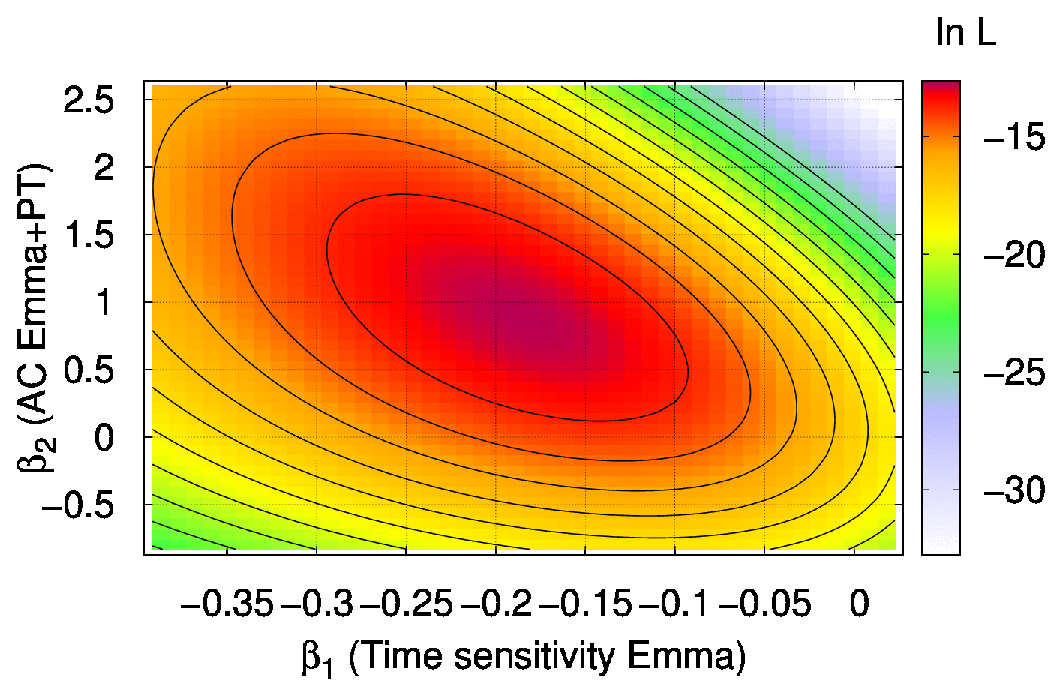
\includegraphics[width=0.5\textwidth]
  {figsDiscr/NL_Skript_2x2alt.Nest1_lnL_beta0_beta1.eps}
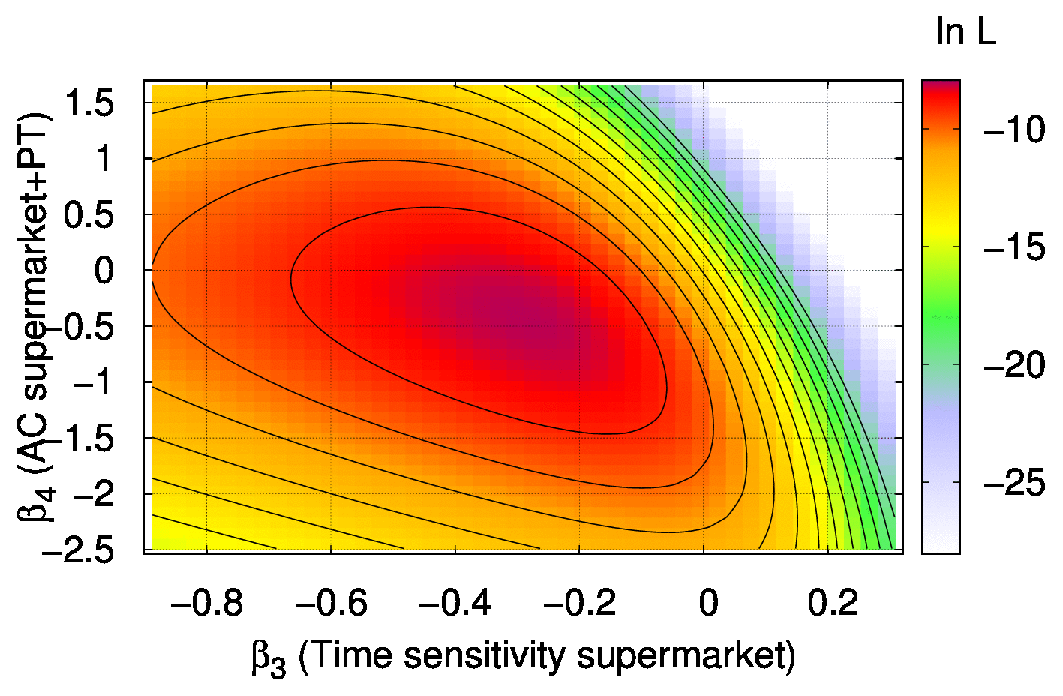
\includegraphics[width=0.5\textwidth]
  {figsDiscr/NL_Skript_2x2alt.Nest2_lnL_beta0_beta1.eps}
\caption{\label{fig:nestedLogit-logL}Log-Likelihood der
  Nest-Nutzenfunktionen~\refkl{NLBeispiel-Nest1} und \refkl{NLBeispiel-Nest2} 
zur Tabelle~\ref{tab:nestedLogit}.
Links: Log-Likelihood der bedingten Verkehrsmittelwahl f\"ur Ziel
``Tante Emma'', rechts f\"ur den Discounter.
 Der Abstand zwischen zwei
H\"ohenlinien entspricht einer Log-Likelihood-Differenz von 1
}
\end{figure}
%###################################################

\bdm
\hatbeta_1=-0.18, \quad
\hatbeta_2=+0.88, \quad
\hatbeta_3=-0.29, \quad
\hatbeta_4=-0.42.
\edm
\bi
\item Die Zeitsensitivit\"aten haben das korrekte (negative) Vorzeichen und
die Sensitivit\"at beim ``Tante-Emma''-Einkauf ist
betragsm\"a\3ig etwas niedriger, allerdings nicht signifikant (weniger
als zwei Log-Likelihood-Einheiten Unterschied in
Abb~{fig:nestedLogit-logL} bei den jeweils anderen Werten von
$\beta_1$ bzw. $\beta_3$).
\item Die AC ist beim ``Tante-Emma''-Einkauf positiv (\"OV gegen\"uber
  dem Auto bevorzugt), beim Discounter dagegen nicht: Dies ist
  plausibel, denn beim Discounter  kauf man i.A.
  viel ein und dann ist ein Auto einfach praktischer.
\ei
Mit den kalibrierten Nest-Parametern lassen sich f\"ur alle $n=10$
Personengruppen die Inklusionsvariablen beider Nests berechnen:
\bdma
I_{n1} &=& \ln\left[\sum_m\exp\frac{\tilV_{n1m}}{\lambda_1}\right]
 = \ln\left[
  \sum_m \exp\left(\hatbeta_1 T_{n1m}+\hatbeta_2 \delta_{m1}\right)\right],\\
I_{n2} &=& \ln\left[\sum_m\exp\frac{\tilV_{n2m}}{\lambda_1}\right]
  = \ln\left[
  \sum_m \exp\left(\hatbeta_3 T_{n2m}+\hatbeta_4 \delta_{m1}\right)\right].\\
\edma
Beispielsweise ergeben sich f\"ur die erste Gruppe $n=1$ und Nest $l=1$
die Nutzenfunktionen $\tilV_{111}/\lambda_1=-3.72$ und
$\tilV_{112}/\lambda_1=-2.77$ und daraus die Inklusionsvariable
$I_{11}= -2.44$. Wie zu erwarten, ist die Inklusionsvariable $I_{11}$
geringf\"ugig gr\"o\3er (hier weniger negativ) als das Maximum der
beiden reduzierten Nutzenfunktionen $\tilV_{111}/\lambda_1$ und
$\tilV_{112}/\lambda_1$. 

%###################################################
\begin{figure}
\fig{0.7\textwidth}{figsDiscr/NL_Skript_2x2alt.Nest1_fProb.eps}
\caption{\label{fig:nestedLogit-Nest1}Verkehrsmittelwahl bei der Fahrt
  zu ``Tante Emma'': Beobachtete relative
  H\"aufigkeiten (Symbole) und durch das NLM modellierte
  Wahrscheinlichkeiten $P_{nm|l=1}$.
}
\end{figure}
%###################################################


%###################################################
\begin{figure}
\fig{0.7\textwidth}{figsDiscr/NL_Skript_2x2alt.Nest2_fProb.eps}
\caption{\label{fig:nestedLogit-Nest2}Verkehrsmittelwahl bei der Fahrt
  zum Discounter: Beobachtete relative
  H\"aufigkeiten (Symbole) und durch das NLM modellierte
  Wahrscheinlichkeiten $P_{nm|l=2}$.
}
\end{figure}
%###################################################


%###################################################
\begin{figure}
\fig{0.7\textwidth}{figsDiscr/NL_Skript_2x2alt.Toplevel_fProb.eps}
\caption{\label{fig:nestedLogit-Toplevel}Wahl des Ladentyps: Beobachtete relative
  H\"aufigkeiten (Symbole) und durch das NLM modellierte
  Wahrscheinlichkeiten $P_{nl}$.
}
\end{figure}
%###################################################

%###################################################
\begin{figure}
\fig{0.7\textwidth}{figsDiscr/NL_Skript_2x2alt.NL_fProb.eps}
\caption{\label{fig:nestedLogit-NL}Kombinierte Entscheidung Ladentyp
  und Verkehrsmittel: Beobachtete relative (kumulierte)
  H\"aufigkeiten (Symbole) und durch das NLM modellierte
  Wahrscheinlichkeiten $P_{nl} P_{nm|l}$.
}
\end{figure}
%###################################################

Mit bekannten Inklusionsvariablen hat man nun ein parameterlineares
MNL-Modell f\"ur die Top-Level-Entscheidung der bin\"aren Ladenwahl
mit dem deterministischen Nutzen
\be
\label{NLBeispiel-Toplevel}
W_{nl}=\beta_5 F_n \delta_{l1} + \beta_6 \delta_{l1} 
  + \lambda_1 I_{nl} \delta_{l1} + \lambda_2 I_{nl} \delta_{l2}.
\ee
Neben der obligaten alternativenspezifischen Konstanten $\delta_{l1}$
und dem zugeh\"origem Parameter $\beta_6$ (globaler Vorteil f\"ur
Tante Emma gegen\"uber dem Discounter bei 
leerem K\"uhlschrank und verschwindenden Zeiten) muss der F\"ullstand
als sozio\"okonomische Variable ebenfalls alternativenspezifisch
formuliert werden. Die Inklusionsvariablen stellen
Charakteristika der Top-Level-Alternativen dar und k\"onnen als solche
generisch (ein $\lambda$) oder alternativenspezifisch ($\lambda_1$ und
$\lambda_2$ mit entsprechenden Selektoren) formuliert werden. Hier
wurde letzteres angenommen. Die ML-Parametersch\"atzung ergibt
%
\bdm
\hatbeta_5=2.9, \quad
\hatbeta_6=-2.0, \quad
\hat{\lambda}_1=0.17, \quad
\hat{\lambda}_2=0.21.
\edm
%
Die Werte sind plausibel:
\bi
\item $\hatbeta_5$ signifikant $>0$: 
Der relative Nutzen des ``Tante-Emma''-Ladens gegen\"uber dem
  Discounter steigt mit dem F\"ullstand des K\"uhlschranks: Ist dieser
  noch fast voll, ist es nicht sinnvoll, beim Discounter gr\"o\3ere Mengen
  einzukaufen.\footnote{Man k\"onnte noch ein drittes triviales Nest
    (``gar nicht einkaufen'') zur Top-Level-Entscheidung
    hinzuf\"ugen.}
\item  $\hatbeta_6$ signifikant $<0$: Bei leerem K\"uhlschrank ist
  hingegen der Discounter ``Tante Emma'' eindeutig vorzuziehen
\item  $\hat{\lambda}_1$ und $\hat{\lambda}_2$ liegen beide im
  geforderten Bereich [0,1],\footnote{Bei der Sch\"atzung k\"onnen aber
    durchaus auch ``verbotene'' Werte vorkommen, diese sollten
    allerdings innerhalb der Sch\"atzunsicherheit von den Grenzen abweichen.}
  aber n\"aher an 0: Der Zufallsnutzen der Top-Level-Nutzenfunktion
  (unbeobachtete Faktoren bei der Ladenwahl) ist deutlich h\"oher als
  der der Verkehrsmittelwahl;  der
  Gesamt-Zufallsnutzen zwischen \"OV und MIV bei gegebenem Ladentyp
  hat eine hohe positive Korrelation.
\ei
Mit dem nun vollst\"andig gesch\"atzten Modell kann man schlie\3lich
noch die Fitg\"ute durch Vergleich der bei den Gruppen vorgefundenen
relativen H\"aufigkeiten mit den modellierten Wahrscheinlichkeiten
absch\"atzen (Abb.~\ref{fig:nestedLogit-Nest1},
\ref{fig:nestedLogit-Nest2}, \ref{fig:nestedLogit-Toplevel}
und~\ref{fig:nestedLogit-NL}).


 

\aufgabenbox{Aufgabe:}{Modellieren Sie dieses Beispiel mit einem
  normalen MNL und definieren Sie dabei die Nutzenfunlktion so, dass
  die Parameter $\beta_1$ bis $\beta_6$ dieselbe Bedeutung haben.}




%#######################################
\subsection{\label{sec:GEVother}Weitere GEV-Modelle}
%#######################################

Zwei weitere h\"aufig benutze GEV-Varianten sind die \bfdef{Paired
  Combinatorial Logit (PCL)} und \bfdef{Generalized Nest Logit (GNL)}
Modelle. Beide Modelle haben eine Nest-Struktur, jedoch kann eine
Alternative Mitglied mehrerer Nests sein. Dies ist vorteilhaft, wenn
eine Abh\"angigkeitstsstruktur nicht streng hierarchisch ist. 

\emph{Beispiel:} Bei
einer Verkehrsmittelwahl mit den Alternativen Fuss, Rad, Bus, Bahn,
MIV-Fahrer und
MIV-Mitfahrer w\"urde man im NL-Modell ein Nest ``MIV'' f\"ur
MIV-Fahrer und -Mitfahrer (gemeinsame unbeobachtete
``Auto-Merkmale''), ein Nest ``\"OV''
f\"ur Bus und Bahn (gemeinsame unbeobachtete \"OV-Merkmale'') sowie
zwei triviale Nests  f\"ur Fuss und Rad ansetzen. Man k\"onnte auch
Fu\3 und Rad zu einem Nest ``sportlicher Modus'' zusammenfassen, da es
gemeinsame unbeobachtete 
``Schlechtwetter'' und ``k\"orperliche Anstrengungsmerkmale''
gibt. Bei diesem Ansatz missachtet man jedoch, dass die Alternative
``MIV-Mitfahrer'' viele mit dem \"OV gemeinsame Merkmale hat,
insbesondere den Mangel an Privatsp\"are und an Flexibilit\"at (der
``Lift'' f\"ahrt zu 
einer festen Zeit los). Also w\"are es g\"unstig, wenn die Alternative
``MIV-Mitfahrer'' gleichzeitig Mitglied der Nester ``MIV'' und \"OV''
sein k\"onnte.


\subsubsection{Paired Combinatorial Logit}
Hier  werden die $I$ Alternativen zu $I(I-1)/2$ Paaren zusammengefasst,
so dass jede Alternative paarweise mit jeder anderen korreliert ist.
Das PCL  wird durch
\be
\label{PCL-G}
G\sup{PCL}(\vec{y})=\sum_{i=1}^{I-1} \sum_{j=i+1}^I
 \left(y_i^{1/\lambda_{ij}} +
 y_j^{1/\lambda_{ij}}\right)^{\lambda_{ij}}
\ee
definiert. Formal hat jeder Summand die Struktur eines NL-Nests mit
zwei Alternativen (``Paar''). Allerdings ist hier jede Alternative
gleichzeitig Mitglied von $I-1$ Paaren anstelle von genau einem Nest
im NL-Modell. 

\subsubsection{Generalized Nest Logit }
Das NL-Modell wird im Generalized Nest Logit (GNL) in zweierlei Hinsicht verallgemeinert:
\bi
\item Jede Alternative kann Mitglied mehrerer Nests sein
\item Der ``Grad der Mitgliedschaft'' (von ``blo\3er Sympathisant''
  bis ``eingetragenes Mitglied'') kann stufenlos gew\"ahlt werden. 
\ei
Die GEV-Funktion des GNL lautet
\be
\label{GNL-G}
G\sup{GNL}(\vec{y})=\sum_{l=1}^L 
 \left(\sum_{i \in B_l} (\alpha_{li} y_i)^{1/\lambda_l}\right)^{\lambda_l}
\ee
Hierbei bezeichnet $B_l$ die Menge der Mitglieder in
Nest $l$  und  $\alpha_{li}$ den
Zugeh\"origkeitsgrad der 
Alternative $i$ zu Nest $l$. Jede Alternative muss Mitglied in mindestens einem Nest sein.
\bi
\item Gibt es $I(I-1)/2$ Nests mit je zwei Mitgliedern
  unterschiedlicher Paarungen und sind alle $\alpha_{li}=1$, so wird das GNL
  zum PCL,
\item sind die $B_l$ exklusiv und vollst\"andig (jedes $i$ ist
  Mitglied in genau einem Nest) und ist $\alpha_{li}=1$, so wird das GNL
  zum NL,
\item hat dar\"uberhinaus jedes Nest nur ein Mitglied oder sind alle
  $\lambda_l=1$, so degeneriert das GNL weiter zum MNL
\ei


%\newpage
%#########################################################
\section{\label{sec:mixed} Mixed-Logit Modell}
%##########################################################
\EinsteinBeg

\providecommand{\vectheta}{\vec{\theta}}

Die Klasse der \bfdef{Mixed-Logit-Modelle}  enth\"alt stochastische
Modellparameter mit vorge\-ge\-bener Verteilung der Dichte
$f(\vecbeta)$.
 Die Auswahlwahrscheinlichkeit 
\be
\label{P-MILO}
P_{ni}=\int\!\! \diff{\vecbeta} f(\vecbeta) P_{ni}\sup{MNL}(\vecbeta)
\ee
ist ein gewichtetes Mittel der normalen
Logit-Auswahlwahrscheinlichkeiten f\"ur bestimmte $\vecbeta$,
gewichtet \"uber die vorgegebene Verteilung der $\vecbeta$  mit Dichte
$f(\vecbeta)$.

\maintext{Mixed-Logit-Modelle entsprechen einer
``Mischung'' von normalen, mit verschiedenen $\vecbeta$ 
parametrisierten Logit-Modellen, wobei die Wichtung der verschiedenen
Parametervektorwerte durch
die Dichtefunktion bzw. \bfdef{mixing function} $f(\vecbeta)$
gegeben ist.}
%
In der Praxis gibt
man meist die Form der Verteilng vor (z.B $\beta_j \sim N(\mu_j,
\sigma_j^2)$) und kalibriert die Parameter der \emph{mixing function}, also
ermittelt z.B. die Sch\"atzer $\hat{\mu}_j$ und $\hat{\sigma}_j^2$
f\"ur alle $j$. 
Es gibt zwei Interpretationsm\"oglichkeiten desselben Modells:
\bi
\item [I] \bfdef{Taste-Variation}, also unterschiedliche Vorlieben f\"ur
  jede Person (\emph{Kenneth E. Train}, Kap. 6.2). Dieser
  Interpretation liegt auch der Name  dieser
  Modellklasse zugrunde,
\item [II] \bfdef{verallgemeinerte Zufallsnutzen}, welche nicht iid Gumbel sind
(Kap. 6.3). Dabei trennt man einfach von den stochastischen Parametern $\beta_j$
den Erwartungs\-wert $\mu_j$ ab und schl\"agt den Streuanteil dem Zufalls\-nutzen
zu. Damit hat man ein gew\"ohnliches Logit mit festen Parametern
$\vec{\mu}$, aber zus\"atzlich zu den
i.i.d. gum\-belverteilten Zufalls\-nutzen des Logitmodells einen weiteren
nicht-iid, nicht-gum\-bel\-ver\-teil\-ten Zufalls\-nutzen\-anteil, den man
beliebig w\"ahlen kann.
\ei
Des Weiteren hat diese Modellklasse folgende Eigenschaften:

\bi
\item Im Sonderfall, dass nur die alternativenspezifischen Konstanten
  (ACs) stochastisch modelliert werden, modelliert man in der
Interpretation als \emph{Taste-Variation} unterschiedliche globale Bevorzugungen
verschiedener Personen, in der Interpretation als verallgemeinerte
Zufallsnutzen zus\"atzliche 
nicht-Gumbel, nicht-i.i.d  Zufallsnutzen, welche zwischen den
Personen, nicht aber  mit den  exogenen Variablen
korrelieren k\"onnen.

\item F\"ur das Mixed-Logit-Modell gilt i.A. nicht mehr die
  IIA-Auswahl-Verschiebungs\-regel (\emph{substitution pattern}),
  Genaueres in \emph{Train}, Kap. 6.4.

\item Durch einen ``Skalentrick'' kann man
  jedes beliebige \bfdef{Random-Utility Model} 
  (RUM), z.B. das Probit-Modell, als Mixed-Logit-Modell schreiben
  (siehe \emph{Train}, Kap. 6.5): Dazu macht man in der obigen
  Interpretation II 
  die verallgemeinerte Zufallsnutzen sehr viel gr\"o\3er als die
  normalen i.i.d. Gumbel-Zufallsnutzen
  $\epsilon$, l\"asst also den Gumbel-Skalenparameter  $\lambda\to \infty$
  gehen anstatt den Standardwert $\lambda=1$ anzusetzen. 

\ei



%########################################################
\subsection{Paneldaten}
%########################################################

Der begriff \bfdef{Panel} bezieht sich, wie \"ublich, auf die mehrfache Befragung
derselben Personen. In diesem Sinne sind Stated-Choice-Untersuchungen
mit mehr als einem Choice Set pro Person
(also der Art, wie ich sie in der Vorlesung machte) stets Panel-Befragungen. Ein konkret
von einer Person beantwortetes Choice Set hat daher statt $n$ zwei Indices:
\bi
\item den Personenindex $n$,
\item zus\"atzlich den Choice-Set-Index $t$.\footnote{Die Bezeichnung $t$ kommt von der
  urspr\"unglichen Form der Panelbefragunng, also Befragung derselben
  Person an mehreren Zeitpunkten $t$.}
\ei
Im normalen Logit-Modell kann man die mit ein
und derselben Person einhergehenden Korrelationsanteile nicht
unterbringen: Jedes konkret beantwortete Choice Set $(n,t)$ ist
unabh\"angig und wird so behandelt, als ob jede Person nur ein
einziges  Choice Set  beantworten w\"urde.

Im Mixed-Logit-Modell kann man die Korrelationen ausnutzen, indem man
gem\"a\3 
Interpretation~I (\emph{Taste-Variation}) den totalen Nutzen ansetzt als
\be
U_{nti}=\vecbeta_n\tr \vec{x}_{nti} + \epsilon_{nti}.
\ee
Der Parametervektor $\vecbeta$ h\"angt also von der Person $n$ ab.
Gem\"a\3 Interpretation~II (Nicht-Gumbel-Anteile der Zufallsnutzen)
setzt man 
\be
\label{transScale}
U_{nti}=\vecbeta\tr \vec{x}_{nti} + \vec{\sigma}\tr \vec{\eta}_n
\vec{x}_{nti}+ \epsilon_{nti},
\ee
wobei $\vec{\sigma}$ den Standardabweichungsvektor und
 $\vec{\eta}_n$ den f\"ur Person $n$ 
realisierten Zufallsvektor aus einer Einheitsverteilung 
(z.B. Standardnormal) kennzeichnet.\footnote{Hier wurden keine Kovarianzen zwischen
  Parametern zugelassen, sonst 
muss man eine ganzen Kovarianzmatrix sch\"atzen, was prinzipiell
(jedoch selten in der Praxis) auch geht.} Zu sch\"atzen gibt es also
nicht nur die \"uber alle Personen gemittelten Parameter $\vecbeta$
(bzw. den Erwartungswert $\vec{\mu}$ der personenabh\"angigen
Parametervektoren), sondern auch die Varianzen $\hat{\sigma}_j^2$ der
Schwankungen $\vecbeta_n-\vecbeta$ bzw. $\vecbeta_n-\vec{\mu}$ von Person zu
Person.


%########################################################
\subsection{Parametersch\"atzung des Mixed-Logit-Modells}
%########################################################

Wie bei allen Modellen der diskreten Wahltheorie wird die
Likelihoodfunktion minimiert, also nach~\refkl{LAllg}
mit~\refkl{P-MILO}: 
\be
\label{LMix}
L(\vectheta)=\prod_n P_{ni_n}(\vectheta)
=\prod_n 
\int\!\! \diff{\vecbeta} f(\vecbeta|\vectheta) P_{ni_n}\sup{MNL}(\vecbeta)
\ee
wobei  $i_n$ die bei Person $n$ beobachtete Wahlentscheidung ist.
Hier wurde Unabh\"angigkeit bez\"uglich der Personen vorausgesetzt.
Man beachte, dass die Likelihoodfunktion nun in Abh\"angigkeit der
Parameter  $\vecbeta$ der \emph{Dichtefunktion} $f(\vecbeta)$ des
urspr\"unglichen Parametervektors gegeben ist,
nicht mehr als Funktion des Parametervektors $\vecbeta$ selbst. Wie
oben bereits erw\"ahnt, enth\"alt der Vektor $\vectheta$ in den
meisten Modellierungen die Erwartungswerte und Varianzen der
urspr\"unglichen Parameter.   

Generell gibt es zwei Ans\"atze, $L(\vectheta)$
bzw. $\tilL(\vectheta)=\ln L(\vectheta)$ zu berechnen (und zu
maximieren):

\bi
\item Direkte numerische Integration, z.B. durch Trapezregel. (Geht in
  \texttt{Python-Biogeme} durch fertige Routinen). Dies ist meist nur f\"ur
  einen stochastischen Parameter sinnvoll,
\item Monte-Carlo-Simulation bei $\ge 2$ stochastischen Parametern:
\be
P_{ni}=\int \diff{\vecbeta} f(\vecbeta) P_{ni}\sup{MNL}(\vecbeta)
\approx \frac{1}{R} \sum_{r=1}^R 
P_{ni}\sup{MNL}(\vecbeta_r) \equiv P_{ni}\sup{num},
\ee
wobei $\vecbeta_r$ eine Realisierung (``Ausw\"urfeln'') der mehrdimensionalen
Zufallsvariable $\vecbeta$ mit Dichte $f(\vecbeta)$
darstellt. Auch daf\"ur liegen in \texttt{Biogeme} fertige Routinen
vor.\footnote{Die Zahl $R$ der n\"otigen \emph{draws} ist in \texttt{Biogeme}
  nicht dokumentiert. $R\ge 1\,000$ ist plausibel, f\"ur
  vieldimensionale Probleme auch deutlich mehr.}

Bei der eigentlichen Optimieruing ist wichtig, dass das
``Ausw\"urfeln'' der $\vecbeta_r$ nur bei der ersten Berechnung der
Likelihood (mit den Startwerten von $\vectheta$) geschieht, z.B. indem
man im Ansatz $\vecbeta(\vectheta)=\vec{\mu}+\vec{\sigma}\eta$ nur
Realisierungen $\eta_r$ der Standardverteilung
(z.B. Standardnormalverteilung) ``ausw\"urfelt'' und im Verlauf der
eigentlichen Maximierung bez\"uglich $\vectheta$ (siehe
auch~\refkl{transScale})  die Werte $\vecbeta_r=\vec{\mu}+\vec{\sigma}\eta_r$
durch Verschiebung (\"Anderung der Komponenten $\mu_j$ von $\vectheta$)
bzw. Skalierung (\"Anderung der Komponenten $\sigma_j^2$ von
$\vectheta$) ermittelt: Andernfalls ist $L(\vectheta)$ nicht bez\"uglich
$\vectheta$ differenzierbar, was die Optimierung erschwert.
\ei




%########################################################
\subsection{Spezialfall: Sch\"atzung bei einer Panel-Struktur} 
%########################################################

In der allgemeinen Likelihood~\refkl{LMix} ist zwar prinzipiell auch
eine Panelstruktur einbaubar, indem man die Parameter-Verteilungen
$f(\vecbeta|\vectheta)$ von der Person $n$ abh\"angen l\"asst, also
$f_n(\vecbeta|\vectheta)$ 
(z.B. f\"ur jede Person einen eigenen deterministischen Wert), aber
das vervielfacht die Zahl der Modellparameter.\footnote{Im Extremfall
  l\"auft es auf die separate Sch\"atzung des Modells f\"ur jede
  Person $n$ heraus.}

Gebr\"auchlicher ist deshalb das Vorgehen nach
Abschnitt (6.7), v.A. Gl (6.2) und (6.3), des Lehrbuchs von
\emph{Train}: Eine 100\%ige Korrelation von $\vecbeta$ bez\"uglich der
Choice Sets $t$ einer Person
$n$ wird erreicht, indem das Integral \"uber $f(\vecbeta)$ 
\emph{simultan} f\"ur alle  Choice Sets einer Person durchgef\"uhrt wird, also 
\be
\label{L-MILO-panel}
L\sup{Panel}(\vectheta)
=\prod_n \int\! \diff{\vecbeta} f(\vecbeta|\vectheta)
\prod_t P_{nti_{nt}}\sup{MNL}(\vecbeta)
\ee
Hingegen erh\"alt man bei Annahme der Unabh\"angigkeit zwischen den Choice
Sets (und Personen) 
\be
\label{L-MILO-unabh} 
L\sub{unabh}(\vectheta)
=\prod_n \prod_t 
\left(\int\! \diff{\vecbeta} f(\vecbeta|\vectheta)P_{nti_{nt}}\sup{MNL}(\vecbeta)\right).
\ee
Ohne stochastische Modellparameter, also ohne Integration, gibt es keinen Unterschied.
Mit Integration ergibt sich jedoch ein Unterschied, da das Produkt
\"uber Summen (bzw. Integrale) nach~\refkl{L-MILO-unabh} i.A. nicht
gleich der Summe (bzw. Integral) \"uber Produkte nach~\refkl{L-MILO-panel} ist. 

\subsubsection*{Veranschaulichung des Unterschiedes}
Im einfachsten Fall, der auch gleichzeitig die Monte-Carlo-Simulation
veranschaulicht, werden pro Person $n$ zwei Choice Sets $t=1$ und 2
betrachtet und das Integral durch nur zwei gleichgewichtete Summanden
(Wichtung 1/2)
mit den (von $\vectheta$
abh\"angigen) Parametervektoren $\vecbeta_1$ und $\vecbeta_2$ angen\"ahert. 
Nach~\refkl{L-MILO-panel} ergibt sich 
\bdm
L\sup{Panel}=\prod_n P_n\sup{Panel}
=\prod_n \frac{P_{n11}P_{n21}+P_{n12}P_{n22}}{2},
\edm
nach~\refkl{L-MILO-unabh} hingegen
\bdm
L\sup{unabh}=\prod_n P_n\sup{unabh}
=\prod_n \left(\frac{P_{n11}+P_{n12}}{2}\right)\left(\frac{P_{n21}+P_{n22}}{2}\right),
\edm
wobei die Abk\"urzungen
\bdm
P_{n11}=P_{n1i_{n1}}\sup{MNL}(\vecbeta_1), \quad
P_{n12}=P_{n1i_{n1}}\sup{MNL}(\vecbeta_2), \quad
P_{n21}=P_{n2i_{n2}}\sup{MNL}(\vecbeta_1), \quad
P_{n22}=P_{n2i_{n2}}\sup{MNL}(\vecbeta_2)
\edm
eingesetzt wurden.\footnote{Leider hat
  \emph{Train} in seinem Buch diesen Unterschied, der m.M nach vieles erkl\"art,
nicht explizit gemacht.}


Obige Formel beschreibt auch die tats\"achliche Struktur der numerischen Ann\"aherung
durch ``Simulation'', nur dass die Anzahl $R$ der \emph{draws}
mindestens 1\,000 und nicht 2 betragen sollte.

%#########################################################
%\section{\label{sec:zuverl} Charakterisierung der Zuverl\"assigkeit}
% transferred to Bachelor to replace part of linear models
%##########################################################



%#########################################################
\section{\label{sec:discrHerl}Einige Herleitungen}
%##########################################################
\EinsteinBeg


%#########################################################
\subsection*{Veranschaulichung bzw. direkte Herleitung 
von Gl \protect\refkl{binAllg}}
%#########################################################

F\"ur die Wahrscheinlichkleit $P_1$, von zwei Alternative Alternative
1 auszuw\"ahlen, gilt
\bdma
P_1 &=& P(U_1>U_2) \\
 &=& P(V_1+\epsilon_1>V_2+\epsilon_2) \\
 &=& P(\epsilon_2-\epsilon_1 \le V_1-V_2) \\
&=& \uu{F_{\epsilon_2-\epsilon_1}(V_1-V_2)}.
\edma
Dr\"uckt man nun mit Hilfe der Faltungss\"atze \refkl{Faltung} die
Verteilungsfunktion der Differenz $\epsilon_2-\epsilon_1$ durch die
Verteilungsfunktionen bzw. Dichten der beiden Zufallsnutzen aus,
erh\"alt man den Ausdruck von \refkl{binAllg} f\"ur zwei Alternativen,
$I=2$.

%#########################################################
\subsection*{Herleitung der Gumbelverteilung als Grenzverteilung}
%#########################################################

Zun\"achst wird ein Spezialfall von Verteilungen mit exponentiellem
Abfall betrachtet: Rein exponentialverteilte Zufallsgr\"o\3en
$X_i \sim E(\lambda)$ mit der Verteilungsfunktion 
$F_E(x)=1-e^{-\lambda x}$. Wir betrachten die Verteilungsfunktion
folgender Maximumsfunktion:
\bdm
Y=\max_{i=1, ..., K} X_i, \quad X_i \sim E(\lambda) \ \text{mit} \
 F_E(x)=1-e^{-\lambda x}.
\edm
Dann gilt
\bdm
F_y(y)=P(Y\le y)=P\left( \max_i X_i \le y \right)
=P \bigg ( (X_1 \le y) \cap \ldots \cap  (X_I \le y) \bigg).
\edm
Sind die $X_i$ unabh\"angig, spalten sich die Wahrscheinlichkeit der 
kombinierte Bedingung in multiplikativ verkn\"upfte
Wahrscheinlichkeiten f\"ur die Einzelbedingungen auf. Damit ergibt sich
\bdma
F_y(y) &=& P (X_1 \le y) P(X_2 \le y) \ldots P(X_I\le y) \\
 &=& \prod_i F_i(y) \\
 &=& \left(1-e^{-\lambda y}\right)^I.
\edma
Ist  nun $y$ hinreichend gro\3, so dass 
\be
\label{approxGrenz}
\alpha := e^{-\lambda y}\ll 1,
\ee
 so kann man folgende N\"aherung anwenden:
\bdm
(1+\alpha)\approx e^{\alpha},
\edm
also $1-e^{-\lambda y} \approx \exp(-e^{-\lambda y})$ und damit
\bdma
F_y(y)  &=& \left(1-e^{-\lambda y}\right)^I \\
 &=& \exp \left(-Ie^{-\lambda y} \right) \\
 &=& \exp \left(-e^{-\lambda y+ \ln I} \right) \\
 &=& \exp \left[-e^{-\lambda \left(y- \frac{\ln I}{\lambda}\right)} \right].
\edma
Bei G\"ultigkeit der N\"aherung gilt also 
$Y \sim \text{Gu} (\ln I/\lambda, \lambda)$. Das Maximum ist also
gumbelverteilt mit demselben Skalierungsparameter wie der der
urspr\"unglichen Exponentialverteilung und einem Lageparameter, der
logarithmisch mit der Zahl der zu maximierenden Variablen ansteigt.
Nun muss man noch zeigen
\benum
\item dass bzw wann die N\"aherung \refkl{approxGrenz} g\"ultig ist,
\item dass das Ergebnis auch f\"ur beliebige Verteilungen mit
\textit{exponential tails} g\"ultig ist.
\eenum
\bi
\item[Zu 1.:] 
F\"ur
interessante Werte von $y$ in der N\"ahe des Modalwertes $\eta_y=\ln
I/\lambda$ (vgl. Gl. \refkl{GumbelTransl})
gilt $\alpha=e^{-\lambda y}=1/I$, also ist Bedingung
\refkl{approxGrenz} f\"ur $I\gg 1$ erf\"ullt. 
\item[Zu 2.:] 
Dies gilt auch f\"ur
beliebige exponentiell abfallende Verteilungen, so lange der
\textit{exponential tail} sp\"atestens beim $1-1/I$-Quantil beginnt,
also die Dichte exponentiell abf\"allt f\"ur alle $x$ 
oberhalb des Wertes, f\"ur den $F(x)=1-1/I$
(vgl. Abb. \ref{fig:gumbelGrenz2}). 
\ei


%#########################################################
\subsection*{Herleitung der Identit\"at \protect\refkl{Gumbelii}}
%#########################################################

Sei
\bdm
Y=\max_{i, i=1, ..., I} X_i, \quad X_i \sim \text{Gu}(\eta_i,\lambda).
\edm
Dann gilt, ganz analog wie bei der obigen Herleitung der
Grenzverteilungseigenschaft 
\bdm
F_y(y)=P(Y\le y)=\prod_i F_i(y),
\edm
nur dass die $F_i$ diesmal die Verteilungsfunktionen von 
$(\eta_i,\lambda)$-Gumbelverteilungen darstellen.  Mit
\refkl{FGumbel} ergibt sich
\bdma
F_y(y)
 &=& \prod_i F_i(y) \\
 &=& \prod_i \exp \left[-e^{-\lambda(y-\eta_i)}\right]\\
 &=& \exp \left[- \sum_i e^{-\lambda(y-\eta_i)}\right] \\
 &=& \exp \left[
        -e^{-\lambda y}\left(\sum_i e^{\lambda \eta_i} \right)
         \right]\\
 &=& \exp \left[
        -e^{-\lambda \left[y-\frac{1}{\lambda} 
        \ln \left(\sum_i e^{\lambda \eta_i} \right)\right]}
         \right]
\edma
Vergleich mit \refkl{FGumbel} zeigt, dass $Y=\max_i X_i$
gumbelverteilt ist mit unver\"andertem Skalierungsparameter $\lambda$
und neuem Lageparameter 
\bdm
\eta_y=\frac{1}{\lambda}  \ln \left(\sum_i e^{\lambda \eta_i} \right).
\edm
%
Diese Identit\"at ist auch konsistent mit der Tatsache, dass die
Gumbelverteilung die Grenzverteilung des Maximums vieler
unabh\"angiger Zufallsvariablen mit \textit{exponential tails} ist:
Das Maximum zweier gumbelverteilten Zufallsgr\"o\3en entspricht also
dem Maximum zweier Maxima, also dem Maximum aller durch die
beiden Gumbelverteilungen repr\"asentierten exponentiell abfallenden
Zufallsvariablen, f\"ur die der Grenzwertsatz nat\"urlich auch gilt.

%#########################################################
\subsection*{Herleitung der Identit\"at \protect\refkl{Gumbeliii}}
%#########################################################

Seien zun\"achst zwei identisch gumbelverteilte
Zufallsvariablen $X_1 \sim \text{Gu}(0,\lambda)$ und
$X_2 \sim \text{Gu}(0,\lambda)$ gegeben. Dann gilt f\"ur die
Verteilungsfunktion der Differenz $Y=X_2-X_1$ unter Verwendung 
der Faltungss\"atze \refkl{Faltung}:
\bdma
P(Y<y)= F_y(y) &=& \int \limits_{-\infty}^{\infty} \diff{x} f_1(x)F_2(y+x)\\
&=& \int \limits_{-\infty}^{\infty}  \diff{x}  \lambda e^{-\lambda x}
\exp[-e^{-\lambda x}]\exp[-e^{-\lambda (y+x)}]\\
&=& \int \limits_{-\infty}^{\infty}  \diff{x}  \lambda e^{-\lambda x}
\exp \left[- \left(e^{-\lambda x}+e^{-\lambda (y+x)}\right) \right]\\
&=& \int \limits_{-\infty}^{\infty}  \diff{x}  \lambda e^{-\lambda x}
\exp \left[- e^{-\lambda x}\left(1+e^{-\lambda y}\right) \right]
\edma
Im Integranden steht nun $1/(1+e^{-\lambda y})$ multipliziert mit der
Ableitung von $\exp[- e^{-\lambda x}(1+e^{-\lambda y})]$ nach $x$, also
\bdm
F_y(y)=\frac{1}{ 1+e^{-\lambda y}}
\left[ \exp[- e^{-\lambda x} \left(1+e^{-\lambda x} \right) 
\right]^{x=\infty}_{x=-\infty} = \frac{1}{ 1+e^{-\lambda y}}.
\edm
Verallgemeinert man das Ergebnis nun nachtr\"aglich auf
nichtverschwindende Lageparameter $\eta_1$ und $\eta_2$ f\"ur die
Zufallsvariablen $X_1$ bzw. $X_2$, erh\"alt man mit dem durch 
\refkl{Gumbeli} gegebenen Verschiebungssatzes f\"ur den Lageparameter
direkt die Identit\"at \refkl{Gumbeliii}:
$\tilde{X}_1=X_1+\eta_1$ ist gumbelverteilt mit  dem Lageparameter $\eta=\eta_1$ und  
$\tilde{X}_2=X_2+\eta_2$ gumbelverteilt mit $\eta=\eta_2$. Damit
ist $Y+\eta_2-\eta_1=\tilde{X}_2-\tilde{X}_1$ einerseits die gesuchte Differenz
der Gumbelverteilungen
mit den Lageparametern $\eta_2$ und $\eta_1$. Andererseits gilt
allgemein
\bdm
X \ \text{hat Verteilungsfunktion $F(x)$} \ \Leftrightarrow \ X+a
 \ \text{hat Verteilungsfunktion $F(x-a)$}
\edm
Also hier
\bdm
Y \ \text{hat Verteilungsfunktion} \frac{1}{ 1+e^{-\lambda y}} \ \Leftrightarrow \ 
Y+\eta_2-\eta_1 \ \text{hat Verteilungsfunktion}
\frac{1}{ 1+e^{-\lambda (y-\eta_2+\eta_1)}},
\edm
was der Aussage \refkl{Gumbeliii} entspricht.

%#########################################################
\subsection*{Herleitung der Multinomial-Logit-Wahrscheinlichkeiten
\protect\refkl{MNL} unter Ber\"ucksichtigung der Gumbel-Eigenschaften}
%#########################################################

Hier werden die eben hergeleitete Identi\"aten \refkl{Gumbelii} und
\refkl{Gumbeliii} ausgenutzt. F\"ur die Auswahlwahrscheinlichkeit
$P_1$ gilt
\bdma
P_1&=& P \left(V_1+\epsilon_1 > \max_{i=2, ...,I}(V_i+\epsilon_i)\right) \\
&=& P \left(\epsilon_1>\max_{i=2, ..., I}(\epsilon_i+V_i-V_1)\right).
\edma
Im Logit-Modell sind alle Zufallsnutzen gumbelverteilt: $\epsilon_i
\sim \text{Gu}(0, \lambda)$.\footnote{Den Lageparameter kann man ohne
Einschr\"ankung =0 setzen, da es nur auf Differenzen ankommt.}
Definiert man nun unter Verwendung von \refkl{GumbelTransl} und \refkl{Gumbelii}:
\bdma
X_1 &=& \epsilon_1 \sim \text{Gu}(0, \lambda), \\
X_2 &=& \max_{i=2, ...,I}(\epsilon_i+V_i-V_1)
  \sim \text{Gu}\left(\frac{1}{\lambda}\sum\limits_{i=2}^Ie^{\lambda(V_i-V_1)},
\lambda \right)
\edma
so gilt
\bdm
P_1=P(X_1 \ge X_2)=P(X_2-X_1 \le 0)=F_{x_2-x_1}(0)
\edm
Nun wendet man Beziehung \refkl{Gumbeliii} f\"ur die
Verteilungsfunktion der Differenz $Y=X_2-X_1$ zweier
gumbelverteilten Zufallsvariablen an:
\bdma
P_1 &=& F_{x_2-x_1}(0)\\[0.5em]
 &=& \frac{1}{1+e^{-\lambda 
\left( 0 - \frac{1}{\lambda}\sum\limits_{i=2}^Ie^{\lambda(V_i-V_1)}\right)
}} \\[0.5em]
 &=&  \frac{1}{1+\sum\limits_{i=2}^Ie^{\lambda(V_i-V_1)}} \\[0.5em]
 &=&  \frac{e^{\lambda V_1}}{e^{\lambda V_1}+\sum\limits_{i=2}^Ie^{\lambda V_i }} \\
 &=&  \frac{e^{\lambda V_1}}{\sum\limits_{i=1}^I e^{\lambda V_i }}
\edma
Die Herleitung l\"asst sich analog f\"ur $P_2$, $P_3$ etc machen, so
dass die Auswahlwahrscheinlichkeiten $P_i$ durch  \refkl{MNL}
gegeben sind.

%#########################################################
\subsection*{Direkte Herleitung der Multinomial-Logit-Wahrscheinlichkeiten
\protect\refkl{MNL}}
%#########################################################

Diese elegante Herleitung stammt von Kenneth E. Train\footnote{Kenneth
  E. Train, \emph{Discrete Choice Methods with Simulation}, frei
  verf\"ugbar unter
  \myHyperlink{http://elsa.berkeley.edu/books/choice2.html}{http://elsa.berkeley.edu/books/choice2.html}.
  Kann aber auch als sch\"ones Buch
z.B. \myHyperlink{http://www.amazon.com/Discrete-Choice-Methods-Simulation-Kenneth/dp/0521747384}{hier}
gekauft werden.}
Setzt man in den Integralausdruck~\refkl{multinomAllg} der
Auswahlwahrscheinlichkeit $P_1$ (o.E.d.A) 
f\"ur allgemeine unabh\"angige Zufallsnutzen die Gumbelverteilung ein,
ergibt sich zun\"achst das Integral

\bdma
P_1 &=& \int\limits_{-\infty}^{\infty}
    \prod\limits_{i=2}^I F_i(\epsilon_1+V_1-V_i)
    f_1(\epsilon_1)\diff{\epsilon_1}\\
  &=& \int\limits_{-\infty}^{\infty}
   \prod\limits_{i=2}^I \exp\left(-e^{-(\epsilon_1+V_1-V_i)}\right)
   e^{-\epsilon_1}\exp(-e^{-\epsilon_1})\diff{\epsilon_1}.
\edma
Man sieht, dass der Faktor $\exp(-e^{-\epsilon_1})$ gerade einem
zus\"atzlichen Faktor des Produkts $\prod_{i=2}^I(..)$ f\"ur $i=1$
bedeutet:
\bdm
P_1= \int\limits_{-\infty}^{\infty}
 \prod\limits_{i=1}^I \exp\left(-e^{-(\epsilon_1+V_1-V_i)}\right)
   e^{-\epsilon_1}\diff{\epsilon_1}.
\edm
Nun schreiben wir das Produkt von e-Funktionen als Summe im
Exponenten:
\bdma
P_1 
 &=& \int\limits_{\epsilon_1=-\infty}^{\infty}
   \exp\left(-\sum_{i=1}^I e^{-(\epsilon_1+V_1-V_i)}\right)
   e^{-\epsilon_1}\diff{\epsilon_1}\\
 &=&  \int\limits_{\epsilon_1=-\infty}^{\infty}
   \exp\left(-e^{-\epsilon_1}\sum_{i=1}^I e^{-(V_1-V_i)}\right)
   e^{-\epsilon_1}\diff{\epsilon_1}.
\edma
Nun kommt der Trick, um dieses Integral auszuf\"uhren: Substituiere
$t=e^{-\epsilon_1}$, $\diff{t}=-e^{-\epsilon_1}\diff{\epsilon_1}$. Die
Integrationsgrenzen werden damit zu
\bdma
\epsilon_1=-\infty &\Rightarrow & t=\infty,\\
\epsilon_1=+\infty &\Rightarrow & t=0.
\edma
also
\bdma
P_1 
 &=& \int\limits_{t=\infty}^0 
   \exp\left(-t\sum_{i=1}^I e^{-(V_1-V_i)}\right)
   (-\diff{t})\\
 &=& \int\limits_{t=0}^{\infty}
   \exp\left(-t\sum_{i=1}^I e^{-(V_1-V_i)}\right)
   \diff{t}\\
 &=& \left[\frac{-1}{\sum_{i=1}^I e^{-(V_1-V_i)}}
   \exp\left(-t\sum_{i=1}^I e^{-(V_1-V_i)}\right)\right]^{\infty}_0\\
 &=& \frac{1}{\sum_{i=1}^I e^{-(V_1-V_i)}}\\
 &=& \frac{e^{V_1}}{\sum_{i=1}^I e^{V_i}},
\edma
q.e.d. F\"ur $P_2$ usw. geht die Rechnung ganz analog.





%#########################################################
\subsection*{Herleitung der allgemeinen Kalibrierungsbedingungen
\protect\refkl{kalibMNLAllg} f\"ur das MNL-Modell}
%#########################################################
Aus \refkl{lMNLAllg} ergibt sich durch Ableiten
\bdma
\abl{\tilL(\vec{\beta})}{\beta_m} &=& \sum\limits_{n,i} y_{ni}
\left(\abl{V_{ni}}{\beta_m} -\frac{1}{\sum_{i'}e^{V_{i'i}}}
\sum\limits_{i''}e^{V_{ni''}}\abl{V_{ni''}}{\beta_m}
\right)\\
&=& \sum\limits_{n,i} y_{ni} \abl{V_{ni}}{\beta_m}
  - \sum\limits_{n} \left(\sum_i y_{ni}\right)
    \left(\frac{\sum\limits_{i''}e^{V_{ni''}}\abl{V_{ni''}}{\beta_m}}
      {\sum_{i'}e^{V_{ni'}}}\right)
\edma
In der zweiten Zeile haben wir ausgenutzt, dass der zweite Summand der
runden Klammer der ersten Zeile gar nicht von $i$
abh\"angt. Insbesondere k\"onnen wir nun nach~\refkl{defyn} die Summe
\"uber $i$ mit 
$\sum_i y_{ni}=y_n$, also mit 
der Gesamtzahl der Entscheidungen in Personengruppe $n$, identifizieren.
Damit k\"onnen wir die Summe \"uber die Laufvariable $i''$ wieder als
eine \"uber $i$ schreiben:
\bdm
\abl{\tilL(\vec{\beta})}{\beta_m}
 = \sum\limits_{n,i} y_{ni} \abl{V_{ni}}{\beta_m}
  - \sum\limits_{n, i} y_n
    \sum\limits_{i}\left(\frac{e^{V_{ni}}}{\sum_{i'}e^{V_{ni'}}}\right)
   \abl{V_{ni}}{\beta_m}.
\edm
 Nun kann man mit Hilfe von \refkl{MNL} den 
Faktor in der runden Klammer im zweiten Summanden als die MNL-Wahrscheinlichkeit
$P_{ni}$ identifizieren. Damit erh\"alt man
\bdma
\abl{\tilL(\vec{\beta})}{\beta_m} &=& 
\sum\limits_{n,i} y_{ni}\abl{V_{ni}}{\beta_m}
- \sum\limits_{n,i} y_{ni} P_{ni} \abl{V_{ni}}{\beta_m}\\
&=&
\sum\limits_{n,i} \left(y_{ni}-y_nP_{ni}\right)
\abl{V_{ni}}{\beta_m},
\edma
also die Beziehung \refkl{kalibMNLAllg}.


%#########################################################
\subsection*{Herleitung der Beziehung \protect\refkl{mH-MNL} f\"ur die
Elemente der Hessematrix}
%#########################################################

Zun\"achst erh\"alt man durch Ableiten nach der Kettenregel:

\bdma
H_{jm} &=& \ablpart{g_j}{\beta_m} \\
 &=& \abl{}{\beta_m}
\left(\sum\limits_{i}x_{nmi}\,y_i\,P_{ni}(\vec{\beta})-\bar{x}_j\right)\\
 &=& \sum\limits_{i}x_{nmi}\,y_i\,\abl{P_{ni}}{\beta_m}.
\edma
Die Ableitungen der MNL-Wahrscheinlichkeiten nach den Parametern ergeben
sich zu

\bdma
\abl{P_{ni}}{\beta_m} 
&=& \abl{}{\beta_m}\left(\frac{1}{\sum_{i'}e^{V_{i'i}-V_{ni}}}\right)\\
&=& -P_{ni}^2\abl{}{\beta_m}
 \left(\sum_{i'}e^{V_{i'i}-V_{ni}}\right)\\
&=& -P_{ni}^2\sum_{i'}e^{V_{i'i}-V_{ni}}
 \abl{}{\beta_m}\left(V_{i'i}-V_{ni}\right) \\
&=& -P_{ni}^2\sum_{i'}e^{V_{i'i}-V_{ni}}
 \abl{}{\beta_m}\sum\limits_j \beta_m\left(x_{ji'i}-x_{nmi}\right)\\
&=& -P_{ni}^2\sum_{i'}e^{V_{i'i}-V_{ni}}\left(x_{mi'i}-x_{nmi}\right)\\
&=& P_{ni}^2\left(
 x_{nmi} \sum_{i'}e^{V_{i'i}-V_{ni}} - \sum_{i'} x_{mi'i}e^{V_{i'i}-V_{ni}} \right) \\
&=& P_{ni}\left(
 x_{nmi}  -  \sum_{i'} x_{mi'i} P_{i'i} \right).
\edma
Hierbei wurde in der letzten Zeile wieder Gl. \refkl{MNL} f\"ur die
MNL-Wahrscheinlichkeiten mehrfach ausgenutzt:
$\sum_{i'}e^{V_{i'i}-V_{ni}}=1/P_{ni}$ und
$e^{V_{i'i}-V_{ni}}=P_{i'i}/P_{ni}$.
Setzt man die letzte Zeile  in den Ausdruck f\"ur $H_{jm}$ ein, ergibt sich

\bdma
H_{jm} &=& \sum\limits_{n,i}x_{nmi}\,y_i\, P_{ni}\left(
 x_{nmi}  -  \sum_{i'} x_{mi'i} P_{i'i} \right),
\edma
also die Beziehungen \refkl{mH-MNL} des Haupttextes.

%#########################################################
\subsection*{Herleitung der Hessematrixelemente
\protect\refkl{mH-BNL}  f\"ur den binomialen Speziallfall}
%#########################################################
!!!
Wie im Haupottext begr\"undet, kann die gesamte Nutzenfunktion auf
Alternative 1 verlagert werden: 
\bdm
V_{j1i}=\sum\limits_j \beta_m x_{j1i}, \quad V_{2li}=0
\edm
Damit ist auch $x_{2li}=0$ und die Summen $\sum_i$ und $\sum_{i'}$ in
Gl. \refkl{mH-MNL} beschr\"anken sich auf jeweils einen Summanden,
$i=1$. Damit wird \refkl{mH-MNL} zu
\bdma
H_{jm} &=& \sum\limits_{i} x_{j1i}\,y_i\,P_{1i}
 \left(x_{m1i}-x_{m1i}P_{1i}\right) \\
 &=& \sum\limits_{i} x_{j1i}\,y_i\,P_{1i} x_{m1i}(1-P_{1i})
\edma
%
und mit $1-P_{n1}=P_{n2}$ schlie\3lich Beziehung \refkl{mH-BNL}.


\newpage

%#########################################################
\section{\label{sec:discrSymbols}Verwendete Symbole}
%##########################################################

\begin{tabular}{ll}
\varDef{$n =1, \cdots, N$}{Personenindex}
\varDef{$i=1, \cdots, I $}{Index der einzelnen Alternativen}
\varDef{$A_n=\{a_{ni}\}$}{Alternativenmenge f\"ur Person $n$}
\varDef{$j=1, \cdots, J_c$ bzw. $J_S$}{Index der $J_c$ Charakteristika
  (generische exogene Variable) bzw. der
  $J_S$ sozio\-\"okono\-mischen exogenen Variablen}
\varDef{$\vec{C}_{ni} =\{c_{jni}\}$}{Satz der ``Charakteristika''
f\"ur Person $n$ bei Alternative $i$}
\varDef{$\vec{S}_{n} =\{s_{jn}\}$}{Satz von sozio\"okonomischen
Variablen f\"ur Person $n$}\\[0em]

\varDef{$m=1, \cdots, M$}{Index der exogenen parameterlinearen
  Einflussfaktoren}
\varDef{$g_{mi}(\vec{C},\vec{S})$}{Kriteriums-Funktion zum
Bilden des $m$-ten parameterlinearen exogenen 
  Einflussfaktors f\"ur Alternative $i$; 
i.A. nichtlineare Funktionen der Charakteristika und der
  sozio\"okonomischen Variablen}
\varDef{$x_{nmi}$\\$=g_{mi}(\vec{C}_{ni},\vec{S}_i)$}{$m$-ter Einflussfaktor
f\"ur Person $n$ bei Alternative $i$ (exogene Variable der
parameterlinearen deterministischen Nutzenfunktionen)}
\varDef{$\vec{x}_{ni}$}{Vektor aller Einflussfaktoren}
\varDef{$y_{ni}$}{Beobachtete Wahlentscheidung: $y_{ni}=1$, wenn
  Person $n$ Alternative $i$ gew\"ahlt hat, sonst $y_{ni}=0$ (endogene
Variable des vollen stochastischen Modells). $y_{ni}>1$ m\"oglich bei
  Zusammenfassung zu Personengruppen.}
\varDef{$y_n=\sum_i y_{ni}$}{Zahl an Personen bzw. Entscheidungen bei
  aggregierter Darstellung, bei der
  der Index $n$ nicht einzelne Personen sondern Klassen bezeichnet
  (sonst $y_n=1$).}
\varDef{$P_{ni}$}{Wahrscheinlichkeit daf\"ur, dass
Person $n$ Alternative $i$ w\"ahlt (endogene Variable des
deterministischen Teilmodells) }
\varDef{$N_i=\sum_ny_{ni}$}{Gesamtzahl der Entscheidungen f\"ur Alternative $i$}
%\varDef{$y_n$}{Zahl der Wahlentscheidungen bei Person(engruppe) $n$}
%\varDef{$n=\sum_i y_n=\sum_i N_i$}{Gesamtzahl der Wahlentscheidungen}
\\[0em]

\varDef{$U_{ni}=V_{ni}+\epsilon_{ni} $}{Gesamtnutzen als Summe von
  deterministischen Nutzen und Zufallsnutzen}
\varDef{$V_{ni}=\sum\limits_m \beta_mx_{nmi}$\\$=\vec{\beta}\tr\vec{x}_{ni}$}
{Deterministischer Nutzen f\"ur
  Person $n$ bei Alternative $i$ in parameterlineare Formulierung}
\varDef{$\delta_{ij}$}{``Selektor''-Dummyvariable. $\delta_{ij}=1$
  falls $i=j$ und =0 sonst.}
\varDef{$\vec{\beta}=\{\beta_m\}$, $\hatvecbeta$}{Satz von Modellparametern,
  dazugeh\"orige Sch\"atzer}
\end{tabular}

\newpage

\begin{tabular}{ll}
\varDef{$\eta, \lambda$}{Lageparameter (Modalwert) und
Skalierungsparameter (proportional zur inversen Standardabweichung)
der Gumbel-Verteilung}
\varDef{$\sigeps$}{Standardabweichung des Zufallsnutzens}
\varDef{$\Phi(x)$}{(kumulierte) Verteilungsfunktion der
  Standardnormalverteilung}
\varDef{$\epsilon_{nii}^{\text{(mic},x_m)}$\\$=\frac{x_{nmi}}{P_i}
  \ablpart{P_i}{x_{nmi}} $}{Mikroskopische Eigenelastizit\"aten
  bez\"uglich des Faktors $x_m$ f\"ur Person $n$ und Alternative $i$}
\varDef{$\epsilon_{nij}^{\text{(mic},x_m)}$\\$=\frac{x_{nmj}}{P_i}
  \ablpart{P_i}{x_{nmj}}  $}{Mikroskopische Kreuzelastizit\"aten
  bez\"uglich des Faktors $x_m$ f\"ur Person $n$ f\"ur Alternative $i$
  aufgrund Attribut\"anderung der Alternative $j$}
\varDef{$\epsilon_{ii}\sup{(mac,$X_m$)}$\\
 $=\frac{\bar{x}_{mi}}{N_i}\ablpart{N_i}{\bar{x}_{mi}}$}
{Makroskopische Eigenelastizit\"at bez\"uglich des Faktors $x_m$
  ($\bar{x}_{mi}$ ist ein geeignetes gewichtetes Mittel \"uber die
  Einzelattribute der Personen $n$).}
\varDef{$L(\vec{\beta})$}{Likelihoodfunktion}
\varDef{$\tilL(\vec{\beta})=\ln L(\vec{\beta})$}{Log-Likelihood}
\varDef{$\m{H}$}{Hesse-Matrix bzw. Informationsmatrix mit den
  Komponenten $H_{mm'}=-\ablpartmix{\tilL(\hatvecbeta)}{\beta_m}{\beta_{m'}}$}
\varDef{$\m{V}$}{Varianz-Kovarianzmatrix der Parametersch\"atzer}
\varDef{$V(\hatbeta_m)=V_{mm}$}{Varianz von $\hatbeta_m$}
\varDef{$\rho_{mm'}$}{Korrelationskoefizient zwischen den
  Parametersch\"atzern}
\varDef{$z_{q}$}{$q$-Quantil (Inverses der Verteilungsfunktion)
  der Standardnormalverteilung.}
\varDef{$\chi^2_{q,n}$}{$q$-Quantil (Inverses der Verteilungsfunktion)
  der $\chi^2$-Verteilung mit $n$ Freiheitsgraden.}
\varDef{$\alpha$}{Fehlerwahrscheinlichkeit}
\varDef{$\lambda\sup{LR}$}{Test-Statistik des Likelihood-Ratio-Tests
  (doppelte Differenz der Log-Likelihoods des vollen und des
  restringierten Modells).}
\varDef{$\rho^2$, $\bar{\rho}^2$}{Likelihood-Ratio (LR) Index
  bzw. korrigierter LR-Index}
\varDef{$I_l$, $\lambda_l$}{Nested-Logit-Modell: Inklusivwert und
  Logit-Skalenparameter (``Inklusivwertparameter'') des Nests (Gruppe von untergeordneten
  Entscheidungen) $l$}
\end{tabular}
